%%%%% Set up %%%%%

% Set document style and font size
\documentclass[12pt]{article}\usepackage[]{graphicx}\usepackage[]{color}
%% maxwidth is the original width if it is less than linewidth
%% otherwise use linewidth (to make sure the graphics do not exceed the margin)
\makeatletter
\def\maxwidth{ %
  \ifdim\Gin@nat@width>\linewidth
    \linewidth
  \else
    \Gin@nat@width
  \fi
}
\makeatother

\definecolor{fgcolor}{rgb}{0.345, 0.345, 0.345}
\newcommand{\hlnum}[1]{\textcolor[rgb]{0.686,0.059,0.569}{#1}}%
\newcommand{\hlstr}[1]{\textcolor[rgb]{0.192,0.494,0.8}{#1}}%
\newcommand{\hlcom}[1]{\textcolor[rgb]{0.678,0.584,0.686}{\textit{#1}}}%
\newcommand{\hlopt}[1]{\textcolor[rgb]{0,0,0}{#1}}%
\newcommand{\hlstd}[1]{\textcolor[rgb]{0.345,0.345,0.345}{#1}}%
\newcommand{\hlkwa}[1]{\textcolor[rgb]{0.161,0.373,0.58}{\textbf{#1}}}%
\newcommand{\hlkwb}[1]{\textcolor[rgb]{0.69,0.353,0.396}{#1}}%
\newcommand{\hlkwc}[1]{\textcolor[rgb]{0.333,0.667,0.333}{#1}}%
\newcommand{\hlkwd}[1]{\textcolor[rgb]{0.737,0.353,0.396}{\textbf{#1}}}%
\let\hlipl\hlkwb

\usepackage{framed}
\makeatletter
\newenvironment{kframe}{%
 \def\at@end@of@kframe{}%
 \ifinner\ifhmode%
  \def\at@end@of@kframe{\end{minipage}}%
  \begin{minipage}{\columnwidth}%
 \fi\fi%
 \def\FrameCommand##1{\hskip\@totalleftmargin \hskip-\fboxsep
 \colorbox{shadecolor}{##1}\hskip-\fboxsep
     % There is no \\@totalrightmargin, so:
     \hskip-\linewidth \hskip-\@totalleftmargin \hskip\columnwidth}%
 \MakeFramed {\advance\hsize-\width
   \@totalleftmargin\z@ \linewidth\hsize
   \@setminipage}}%
 {\par\unskip\endMakeFramed%
 \at@end@of@kframe}
\makeatother

\definecolor{shadecolor}{rgb}{.97, .97, .97}
\definecolor{messagecolor}{rgb}{0, 0, 0}
\definecolor{warningcolor}{rgb}{1, 0, 1}
\definecolor{errorcolor}{rgb}{1, 0, 0}
\newenvironment{knitrout}{}{} % an empty environment to be redefined in TeX

\usepackage{alltt}

% File path to resources (style file etc)
\newcommand{\locRepo}{csas-style}

% Style file for DFO Technical Reports
\usepackage{\locRepo/tech-report}

% header-includes from R markdown entry
\usepackage{float} \usepackage{xfrac} \usepackage{gensymb} \usepackage{multirow} \usepackage{colortbl} \usepackage{xcolor} \usepackage{bookmark} \usepackage{mathptmx}

%%%%% Variables %%%%%

% New definitions: Title, year, report number, authors
% Protect lower case words (i.e., species names) in \Addlcwords{}, in "TechReport.sty"
\newcommand{\trTitle}{Oceanographic monitoring of the Gully MPA -- A synopsis of data collected by the Atlantic Zone Monitoring Program}
\newcommand{\trYear}{2021}
\newcommand{\trReportNum}{nnn}
% Optional
\newcommand{\trAuthFootA}{Email: \href{mailto:Jeffrey.Jackson@dfo-mpo.gc.ca}{\nolinkurl{Jeffrey.Jackson@dfo-mpo.gc.ca}} \textbar{} telephone: (902) 426-9670}
\newcommand{\trAuthsLong}{Jeffrey W. Jackson\textsuperscript{1}, Erica J. H. Head\textsuperscript{1}, Lindsay I. Beazley\textsuperscript{1}, and Andrew T. Cogswell\textsuperscript{1}}
\newcommand{\trAuthsBack}{Jackson, J.W., Head, E.J.H., Beazley, L.I. and Cogswell, A.T.}

% New definition: Address
\newcommand{\trAddy}{\textsuperscript{1}Ocean and Ecosystem Sciences Division\\
Fisheries and Oceans Canada\\
Bedford Institute of Oceanography\\
P.O. Box 1006\\
Dartmouth, Nova Scotia\\
Canada, B2Y 4A2}

% Abstract
\newcommand{\trAbstract}{In 2004, the Gully was established as Atlantic Canada's first Marine Protected Area (MPA) under Canada's Oceans Act, with the goal of protecting its high biodiversity of cold-water corals and habitat for an endangered population of northern bottlenose whales. While the oceanographic setting of the Gully MPA has been described, little has been done to assess changes in its physical, chemical, or biological properties, a key component of evaluating whether the MPA is meeting its conservation objectives. Since the late 1990's, the Atlantic Zone Monitoring Program (AZMP) has routinely collected hydrographic and biological data within the Gully MPA as part of the program's ancillary objectives. However, these data had yet to be compiled and analyzed for the purpose of long-term environmental monitoring. Through a joint initiative between Fisheries and Oceans Canada's Maritimes Region Canadian Science Advisory Secretariat and the AZMP, we present a compilation and reproducible analysis of the physical, chemical, and biological oceanographic data collected at four fixed sampling stations in the Gully between 2000 and 2018. Average temperature, salinity, dissolved oxygen, and nutrient and chlorophyll \emph{a} collected from CTD profiles and bottle samples were evaluated both within and among stations. Patterns of wet weight biomass and abundance of the most common copepod taxa from zooplankton samples collected from vertical ring net tows were also evaluated. Additionally, differences in sea surface temperature and chlorophyll \emph{a} from satellite-based imagery collected between 1998 to 2018 were examined in order to ascertain whether the surface properties of the MPA are unique relative to adjacent shelf-break areas. The main goal of this report is to provide operational advice for effective monitoring of the Gully's oceanographic properties by the AZMP, with a focus on identifying redundancies and/or gaps in the program's existing monitoring strategy for the MPA. We also provide a preliminary assessment of oceanographic environmental monitoring indicators presented in \protect\hyperlink{ref-kenchington_2010}{Kenchington} (\protect\hyperlink{ref-kenchington_2010}{2010}).}

% Resume (i.e., French abstract)
\newcommand{\trResume}{En 2004, le Gully est devenu la toute première zone de protection marine (ZPM) désignée dans la région de l'Atlantique en vertu de la Loi sur les océans, dans le but de protéger sa grande biodiversité de coraux d'eau froide et l'habitat d'une population de baleines à bec communes en voie de disparition. Bien que le milieu océanographique de la ZPM du Gully ait été décrit, peu de choses ont été faites pour évaluer les changements dans ses propriétés physiques, chimiques ou biologiques, un élément clé pour déterminer si la ZPM atteint ses objectifs de conservation. Depuis la fin des années 1990, le Programme de monitorage de la zone Atlantique (PMZA) recueille régulièrement des données hydrographiques et biologiques dans la ZPM du Gully dans le cadre des objectifs auxiliaires du programme. Ces données n'avaient cependant pas encore été compilées et analysées en vue d'une surveillance environnementale à long terme. Grâce à une initiative conjointe entre le Secrétariat canadien de consultation scientifique de la région des Maritimes de Pêches et Océans Canada et le PMZA, nous présentons une compilation et une analyse reproductible des données océanographiques physiques, chimiques et biologiques recueillies à quatre stations d'échantillonnage fixes dans le Gully entre 2000 et 2018. Les données sur la température moyenne, la salinité, l'oxygène dissous, les nutriments et la chlorophylle \emph{a} qui ont été recueillies au moyen des profils de CTP et des bouteilles d'échantillonnage ont été évaluées à l'intérieur des stations et entre elles. On a également évalué les modèles de poids humide de la biomasse et de l'abondance des taxons de copépodes les plus communs observés dans les échantillons de zooplancton prélevés au moyen de filets à anneaux verticaux. De plus, les différences de température de la surface de la mer et de chlorophylle \emph{a} observées sur les images satellites recueillies entre 1998 et 2018 ont été examinées afin de déterminer si les propriétés de la surface de la ZPM sont uniques comparativement aux zones adjacentes du rebord du plateau continental. Le principal objectif de ce rapport est de fournir des conseils opérationnels pour assurer une surveillance efficace des propriétés océanographiques du Gully par le PMZA, en mettant l'accent sur le recensement des redondances et des lacunes dans la stratégie de surveillance existante du programme pour la ZPM. Nous offrons également une évaluation préliminaire des indicateurs de surveillance de l'environnement océanographique présentés dans \protect\hyperlink{ref-kenchington_2010}{Kenchington} (\protect\hyperlink{ref-kenchington_2010}{2010}).}

\newcommand{\trISBN}{}

\DeclareGraphicsExtensions{.png,.pdf}
%%%%% Start %%%%%

% Start the document
\IfFileExists{upquote.sty}{\usepackage{upquote}}{}

% commands and environments needed by pandoc snippets
% extracted from the output of `pandoc -s`
%% Make R markdown code chunks work
\usepackage{array}
\usepackage{amssymb,amsmath}
\usepackage{color}
\usepackage{fancyvrb}

% From default template:
\newcommand{\VerbBar}{|}
\newcommand{\VERB}{\Verb[commandchars=\\\{\}]}
\DefineVerbatimEnvironment{Highlighting}{Verbatim}{commandchars=\\\{\}}
% Add ',fontsize=\small' for more characters per line
\usepackage{framed}
\definecolor{shadecolor}{RGB}{248,248,248}
\newenvironment{Shaded}{\begin{snugshade}}{\end{snugshade}}
\newcommand{\AlertTok}[1]{\textcolor[rgb]{0.94,0.16,0.16}{#1}}
\newcommand{\AnnotationTok}[1]{\textcolor[rgb]{0.56,0.35,0.01}{\textbf{\textit{#1}}}}
\newcommand{\AttributeTok}[1]{\textcolor[rgb]{0.77,0.63,0.00}{#1}}
\newcommand{\BaseNTok}[1]{\textcolor[rgb]{0.00,0.00,0.81}{#1}}
\newcommand{\BuiltInTok}[1]{#1}
\newcommand{\CharTok}[1]{\textcolor[rgb]{0.31,0.60,0.02}{#1}}
\newcommand{\CommentTok}[1]{\textcolor[rgb]{0.56,0.35,0.01}{\textit{#1}}}
\newcommand{\CommentVarTok}[1]{\textcolor[rgb]{0.56,0.35,0.01}{\textbf{\textit{#1}}}}
\newcommand{\ConstantTok}[1]{\textcolor[rgb]{0.00,0.00,0.00}{#1}}
\newcommand{\ControlFlowTok}[1]{\textcolor[rgb]{0.13,0.29,0.53}{\textbf{#1}}}
\newcommand{\DataTypeTok}[1]{\textcolor[rgb]{0.13,0.29,0.53}{#1}}
\newcommand{\DecValTok}[1]{\textcolor[rgb]{0.00,0.00,0.81}{#1}}
\newcommand{\DocumentationTok}[1]{\textcolor[rgb]{0.56,0.35,0.01}{\textbf{\textit{#1}}}}
\newcommand{\ErrorTok}[1]{\textcolor[rgb]{0.64,0.00,0.00}{\textbf{#1}}}
\newcommand{\ExtensionTok}[1]{#1}
\newcommand{\FloatTok}[1]{\textcolor[rgb]{0.00,0.00,0.81}{#1}}
\newcommand{\FunctionTok}[1]{\textcolor[rgb]{0.00,0.00,0.00}{#1}}
\newcommand{\ImportTok}[1]{#1}
\newcommand{\InformationTok}[1]{\textcolor[rgb]{0.56,0.35,0.01}{\textbf{\textit{#1}}}}
\newcommand{\KeywordTok}[1]{\textcolor[rgb]{0.13,0.29,0.53}{\textbf{#1}}}
\newcommand{\NormalTok}[1]{#1}
\newcommand{\OperatorTok}[1]{\textcolor[rgb]{0.81,0.36,0.00}{\textbf{#1}}}
\newcommand{\OtherTok}[1]{\textcolor[rgb]{0.56,0.35,0.01}{#1}}
\newcommand{\PreprocessorTok}[1]{\textcolor[rgb]{0.56,0.35,0.01}{\textit{#1}}}
\newcommand{\RegionMarkerTok}[1]{#1}
\newcommand{\SpecialCharTok}[1]{\textcolor[rgb]{0.00,0.00,0.00}{#1}}
\newcommand{\SpecialStringTok}[1]{\textcolor[rgb]{0.31,0.60,0.02}{#1}}
\newcommand{\StringTok}[1]{\textcolor[rgb]{0.31,0.60,0.02}{#1}}
\newcommand{\VariableTok}[1]{\textcolor[rgb]{0.00,0.00,0.00}{#1}}
\newcommand{\VerbatimStringTok}[1]{\textcolor[rgb]{0.31,0.60,0.02}{#1}}
\newcommand{\WarningTok}[1]{\textcolor[rgb]{0.56,0.35,0.01}{\textbf{\textit{#1}}}}
\begin{document}

%%%% Front matter %%%%%

% Add the first few pages
\frontmatter

%%%%% Drafts %%%%%

%\linenumbers  % Line numbers
%\onehalfspacing  % Extra space between lines
\renewcommand{\headrulewidth}{0.5pt}  % Header line
\renewcommand{\footrulewidth}{0.5pt}  % footer line
%\pagestyle{fancy}\fancyhead[c]{Draft: Do not cite or circulate}  % Header text

\newcommand{\lt}{\ensuremath <}
\newcommand{\gt}{\ensuremath >}

%Defines cslreferences environment
%Required by pandoc 2.8
%Copied from https://github.com/rstudio/rmarkdown/issues/1649
\newlength{\cslhangindent}
\setlength{\cslhangindent}{1.5em}
\newenvironment{cslreferences}%
  {}%
  {\par}

%%%%% Main document %%%%%
\hypertarget{sec:introduction}{%
\section{INTRODUCTION}\label{sec:introduction}}

\hypertarget{the-gully-marine-protected-area}{%
\subsection{\texorpdfstring{\textbf{THE GULLY MARINE PROTECTED AREA}}{THE GULLY MARINE PROTECTED AREA}}\label{the-gully-marine-protected-area}}

Submarine canyons are common geomorphic features of continental margins worldwide. Their complex topography influences a number of hydrodynamical processes, such as ocean currents, tides, and internal waves, which may have a profound effect on the structure, function, and diversity of their residing pelagic and benthic communities (\protect\hyperlink{ref-kenchington_2014b}{Kenchington et al. 2014b}; \protect\hyperlink{ref-macisaac_2014}{MacIsaac et al. 2014}; \protect\hyperlink{ref-fernandez-arcaya_2017}{Fernandez-Arcaya et al. 2017}). Enhanced species diversity of canyon features has been linked to increased nutrient fluxes generated by upwelling (\protect\hyperlink{ref-freeland_1982}{Freeland and Denman 1982}).

The Gully canyon is the largest submarine canyon on the continental margin of eastern North America (\protect\hyperlink{ref-gordon_2002}{Gordon and Fenton 2002}). Located 40 km east of Sable Island, the Gully incises the Scotian Shelf between Sable Island Bank and Banquereau, is over 65 km long and 15 km wide, and reaches a depth of 2000 m at the shelf break. Since the 1990's, the Gully has been an area of special conservation interest due to its abundance and diversity of benthic features, including cold-water corals and various commercial and non-commercial fish species, and for its diverse community of marine mammals. Fisheries and Oceans Canada (DFO) designated the area a whale sanctuary in 1994 in an effort to reduce ship collisions and noise disturbance for an endangered population of Northern Bottlenose whales that resides there (\protect\hyperlink{ref-dfo_2008}{DFO 2008}). In response to concerns over the impact of various anthropogenic activities, including offshore oil and gas exploration, shipping and commercial fishing activity (\protect\hyperlink{ref-vanderzwaag_2011}{VanderZwaag and Macnab 2011}) in the Gully and on its associated biodiversity, in 2004 DFO established the Gully as Atlantic Canada's first Marine Protected Area (MPA) under Canada's Oceans Act. \href{https://www.dfo-mpo.gc.ca/oceans/mpa-zpm/gully/index-eng.html}{The Gully MPA} encompasses an area of 2364 km\textsuperscript{2}, and is comprised of three different management zones that each have their own set of management measures and levels of protection.

\hypertarget{environmental-monitoring-of-the-gully}{%
\subsection{\texorpdfstring{\textbf{ENVIRONMENTAL MONITORING OF THE GULLY}}{ENVIRONMENTAL MONITORING OF THE GULLY}}\label{environmental-monitoring-of-the-gully}}

In 1998, a comprehensive scientific review of the Gully's environmental and ecosystem characteristics was published in support of MPA planning (\protect\hyperlink{ref-harrison_1998}{Harrison and Fenton 1998}), and included the first synopsis of the Gully's physical oceanographic properties (see \protect\hyperlink{ref-petrie_1998}{Petrie et al. 1998}). Using data archived at the Bedford Institute of Oceanography, patterns in the Gully's observed and modelled circulation, low-frequency current variability and cross-shelf exchange, internal tidal generation, and seasonal and inter-annual variability in hydrographic properties were examined. Some evidence pointing to localized retention of particles within the Gully was presented, which had long been theorized to drive enhanced primary productivity and biodiversity of the Gully (\protect\hyperlink{ref-harrison_1998}{Harrison and Fenton 1998}). However, the authors noted that the conclusions of the circulation models were based on relatively few observations, and that oceanographic data are lacking in the Gully, particularly in its deeper regions. In 2006 and 2007, a high spatial-resolution field program was later conducted in the Gully (see \protect\hyperlink{ref-greenan_2014}{Greenan et al. 2014}; \protect\hyperlink{ref-shan_2014a}{Shan et al. 2014a}, \protect\hyperlink{ref-shan_2014b}{2014b}), where both continuous (i.e., current-meter moorings deployed from April 2006 to August 2007) and discrete (i.e., CTD) observations were collected in order to better describe its mean circulation and evaluate evidence for enhanced mixing, flux, and other physical oceanographic properties that may differentiate the canyon from adjacent shelf and slope areas. These data have since been re-examined for the purpose of providing a comprehensive environmental background of the Gully to assist in the interpretation of catch data from midwater-trawl surveys of the nekton and micronekton at meso- and bathypelagic depths (see \protect\hyperlink{ref-kenchington_2014b}{Kenchington et al. 2014b}).

In 2008, the Gully Marine Protected Area Management Plan (\protect\hyperlink{ref-dfo_2008}{DFO 2008}, \protect\hyperlink{ref-dfo_2017}{2017} second edition) was released, which outlines the conservation, management, and stewardship objectives for the MPA as well as key research and monitoring goals. The overarching conservation objective of the MPA is to ``protect the health and integrity of the Gully ecosystem,'' and is divided into three different sub-objectives:
\begin{enumerate}
\def\labelenumi{\arabic{enumi})}
\item
  Protect the natural biodiversity of the Gully
\item
  Protect the physical structure of the Gully and its physical and chemical properties
\item
  Maintain the productivity of the Gully ecosystem
\end{enumerate}
The Gully Marine Protected Area Management Plan also describes several, high priority conservation objectives, which were intended to be the focus of future monitoring efforts (\protect\hyperlink{ref-dfo_2010}{DFO 2010}):
\begin{enumerate}
\def\labelenumi{\arabic{enumi})}
\item
  Protecting cetaceans from impacts caused by human activities
\item
  Protecting seafloor habitat and associated benthic communities from alteration caused by human activities
\item
  Maintaining or restoring the quality of the water and sediments of the Gully
\item
  Conserving other commercial and non-commercial living resources In order to address these conservation objectives, (\protect\hyperlink{ref-kenchington_2010}{Kenchington 2010}) developed a recommendation for monitoring for the Gully that consisted of 47 indicators and advice on how to implement a cost-effective and efficient monitoring program that incorporated data collected by existing monitoring platforms. Of these 47 indicators, 8 were developed to monitor the physical, chemical, and biological state of the MPA:
\item
  Temperature, salinity, oxygen concentration, alkalinity, pH, light levels, chlorophyll, pigments and nutrients in the water column within the MPA, including in close proximity to the seabed (Indicator 21)
\item
  Temperature, salinity, oxygen concentration, light levels, chlorophyll, pigments and nutrients in waters flowing into and past the MPA, as measured on the Louisbourg Line, the Halifax Line and the Extended Halifax Line (Indicator 22)
\item
  Physical (temperature, salinity, wind, sea-surface height) and biological (ocean colour) sea surface properties in the MPA and the surrounding region (Indicator 23)
\item
  Weather conditions at the Sable Island weather station and at the Banquereau and Laurentian Fan weather-buoy sites, including wind direction and speed, air pressure and sea-level air temperatures, plus for the buoy sites sea surface temperatures, wave height and dominant wave period (Indicator 24)
\item
  Three-dimensional distribution and movements of water masses within and around the MPA (Indicator 25)
\item
  Phytoplankton production, community composition and the timing of the spring bloom in the MPA and the surrounding region (Indicator 26)
\item
  Zooplankton biomass, community composition and the biomass of selected species within the MPA (Indicator 27)
\item
  Acoustic scattering in the water column within the MPA (Indicator 28)
\end{enumerate}
Data on indicators 21, 22, 27, and aspects of indicator 26, are routinely collected during biannual monitoring surveys conducted by the \href{https://www.dfo-mpo.gc.ca/science/data-donnees/azmp-pmza/index-eng.html}{Atlantic Zone Monitoring Program} (AZMP). Initiated in 1998, the AZMP was designed to build upon existing regional monitoring activities with the aim of detecting and tracking climate change and variability in the northwest Atlantic, evaluating changes in physical, chemical and biological ocean properties and predator-prey dynamics of marine resources, thereby enhancing Canada's capacity to understand, describe, and forecast the state of the marine ecosystem (\protect\hyperlink{ref-harrison_2002}{Harrison et al. 2002}). AZMP's sampling scheme in the Maritimes Region involves oceanographic sampling at several high-frequency (biweekly to monthly) fixed coastal stations and biannual sampling along fixed core sections (Cabot Strait Line, Louisbourg Line, Halifax Line, Browns Bank Line); the latter of which may also include opportunistic sampling at stations in the Laurentian Channel, Northeast Channel and Gulf of Maine in support of a number of ancillary research programs and initiatives. Oceanographic sampling includes the collection of CTD profiles and water samples for the determination of physical (T, S), chemical (nutrients, O2, pH, alkalinity) and biological (chlorophyll \emph{a} concentration) variables and vertical ring net tows to determine zooplankton biomass and community composition. The same measurements are also made at random-stratified (by depth) locations during DFO's multispecies groundfish trawl surveys.

At present, the AZMP has four fixed stations within the confines of the Gully MPA that are targeted for sample collection during its biannual surveys (see Figures~\ref{fig:figure1} and~\ref{fig:figure2}). Station GULD\_04, situated above the thalweg (Figure~\ref{fig:figure2}) of the canyon at approximately 1855 m depth, was first occupied and hydrographic data collected during the AZMP Hudson and Parizeau cruises of 1999 and 2000 (see Table~\ref{tab:table1}), which were aimed at collecting acoustic backscatter data for the evaluation of seasonal changes in the abundance and community structure of mesozooplankton, macrozooplankton, and micronekton in the Gully and on western Scotian Shelf and Slope (\protect\hyperlink{ref-sameoto_2002}{Sameoto et al. 2002}). Hydrographic data were first collected at GULD\_03 in 2000, after the acoustic data and BIONESS tows collected in the northern shallow arms of the Gully revealed high euphausiid abundances at this location (\protect\hyperlink{ref-sameoto_2002}{Sameoto et al. 2002}). Stations SG\_23 and SG\_28 on the eastern and western flanks of the Gully mouth, respectively, were later adopted from the high spatial-resolution CTD surveys conducted in the Gully in 2006 and 2007 (\protect\hyperlink{ref-greenan_2014}{Greenan et al. 2014}). As sampling at these stations initially served a purpose other than long-term environmental monitoring, their occupation on an annual basis was not consistent until after 2007.

\hypertarget{gully-data-synthesis-project}{%
\subsection{\texorpdfstring{\textbf{GULLY DATA SYNTHESIS PROJECT}}{GULLY DATA SYNTHESIS PROJECT}}\label{gully-data-synthesis-project}}

Since the environmental setting of the Gully was first described and the recommended environmental monitoring program released, little has been done to assess changes in the physical, chemical, or biological state of the MPA, a key component in evaluating whether the MPA is meeting its conservation objectives. A critical first step towards forming a baseline for on-going future environmental monitoring is to compile, analyze, and interpret the existing data collected within the confines of the Gully MPA (\protect\hyperlink{ref-kenchington_2010}{Kenchington 2010}), a task which, to date, has not yet been undertaken. In 2019, a joint project between DFO's Maritimes Region Canadian Science Advisory Secretariat (CSAS) and the AZMP was initiated entitled ``Synthesis of Gully MPA Oceanographic Monitoring Data,'' with the overall goal compiling existing data collected on the physical, chemical, and biological conditions of the Gully MPA, and identifying patterns that may point to a change in the physical or chemical conditions, and/or productivity of the MPA. Three objectives and two deliverables of the project were outlined:

\hypertarget{objectives}{%
\subsubsection{\texorpdfstring{\emph{Objectives}}{Objectives}}\label{objectives}}
\begin{enumerate}
\def\labelenumi{\arabic{enumi}.}
\item
  Provide a synthesis of the physical, chemical, and biological data collected at the AZMP's four fixed stations in the Gully MPA.
\item
  Identify any gaps or redundancies in the current monitoring protocols and provide recommendations on how to mitigate these gaps.
\item
  Develop scripts, analytical products and a preliminary report that will form the basis of future routine environmental monitoring of the Gully MPA.
\end{enumerate}
\hypertarget{deliverables}{%
\subsubsection{\texorpdfstring{\emph{Deliverables}}{Deliverables}}\label{deliverables}}
\begin{enumerate}
\def\labelenumi{\arabic{enumi}.}
\item
  A technical report describing the AZMP's sampling scheme and data collected at the program's four fixed stations in the Gully MPA. The current sampling scheme, and temporal changes in the physical, chemical, and biological conditions at each station should be evaluated.
\item
  A repository containing all of the data, scripts, analytical products and code for report generation that will serve as the template of future Gully MPA oceanographic reporting.
\end{enumerate}
Here we present the first compilation of the physical, chemical, and biological data collected by the AZMP at the four fixed stations in the Gully MPA. CTD profile data collected from 1999 to 2018 were compiled, and average temperature, salinity, dissolved oxygen, and nutrient and chlorophyll \emph{a} inventories were evaluated both within and among the four stations. In addition to the shipboard samples and data collected by the AZMP, sea surface temperature and chlorophyll \emph{a} extracted from satellite-based imagery collected from 1998 to 2018 were also evaluated. While the datasets were deemed insufficient for climatological calculations for which to assess anomalies, changes in oceanographic conditions over the time period sampled were assessed, and significant trends identified.

The overall goal of the analyses presented in this report is to provide operational advice for effective monitoring of the Gully's oceanographic properties by the AZMP. The discussion section is focused on identifying redundancies and gaps in existing AZMP monitoring protocols for the Gully MPA, including whether the placement and number of stations is adequate for detecting changes in oceanographic conditions within its confines.

Additionally, we provide the first preliminary assessment of the oceanographic environmental monitoring indicators presented in \protect\hyperlink{ref-kenchington_2010}{Kenchington} (\protect\hyperlink{ref-kenchington_2010}{2010}). Aspects of Indicators 21, 22, 23, 26, and 27 are evaluated and discussed herein.

\clearpage

\hypertarget{sec:data}{%
\section{DATA AND METHODOLOGY}\label{sec:data}}

\hypertarget{sec:physical-data}{%
\subsection{\texorpdfstring{\textbf{PHYSICAL}}{PHYSICAL}}\label{sec:physical-data}}

\hypertarget{data-collection-and-compilation}{%
\subsubsection{\texorpdfstring{\emph{Data collection and compilation}}{Data collection and compilation}}\label{data-collection-and-compilation}}

A data selection exercise was undertaken to extract all CTD casts conducted at or within the vicinity of the current nominal coordinates of the four monitoring stations in the Gully MPA. Extracting the data using spatial criteria was necessary as station names were often not consistently provided for CTD deployments conducted prior to 2013. Initially, all CTD profiles collected within 2.25 km (to account for vessel drift) of the nominal coordinates of each of the four AZMP fixed stations were queried and extracted from the Ocean Data and Information Section (ODIS) CTD Archive, a local, shared network drive used to house all CTD data collected by the AZMP. After this extraction revealed a low number results, all profiles assigned with the desired station name were queried and extracted from the archive, regardless of distance from the nominal station location. All profiles resulting from the above extractions were plotted using ArcMap GIS software (version 10.7.1) and their placement in relation to the nominal station coordinates and nearby topographic features (e.g.~shallow banks) were evaluated. Some profiles conducted on the shallow bank within the immediate vicinity of GULD\_03 were removed, as the hydrographic conditions were likely different from those occurring closer to the canyon thalweg where GULD\_03 is located. A cluster of CTD casts located approximately 3 km to the northwest of GULD\_03 was retained, as this location likely served as the former nominal location for station GULD\_03.

The maximum depth of each profile was then evaluated against both the nominal station depth based on the General Bathymetric Chart of the Oceans (GEBCO) 2019 bathymetric data, and the total water depth based on ship's sounding. Profiles with a maximum depth of 200 m or greater than the nominal station depth were not considered further. Profiles that were aborted at the surface were removed, as were profiles that reached water depths ≥200 m than the nominal station depth based on GEBCO. Four additional CTD profiles collected in March 2010 during a survey to quantify the mesopelagic communities of the Gully were also excluded from all subsequent analyses.

This data reduction exercise resulted in a total of 89 profiles collected across all four monitoring stations between 1999 and 2018 (see Table~\ref{tab:table1} and Figure~\ref{fig:figure2}). The majority of the profiles were collected during AZMP's biannual surveys, while others were collected during the targeted oceanographic survey of \protect\hyperlink{ref-greenan_2014}{Greenan et al.} (\protect\hyperlink{ref-greenan_2014}{2014}). While the four AZMP fixed stations have been occasionally sampled during DFO's multispecies research vessel trawl survey, those profiles were not considered to meet the data selection criteria described above, and are consequently not included in this report.

A similar data exercise was undertaken to extract the CTD profile data collected from AZMP core stations on the Louisbourg and Halifax Lines, in order to capture waters flowing into (Louisbourg Line, upstream of the Gully) and past the MPA (Halifax Line, downstream of the Gully), and to compare their conditions with those in the Gully MPA. CTD profiles collected during the AZMP biannual surveys conducted between 2000 to 2018 collected at the Louisbourg Line station LL\_07 (nominal depth approximately 760 m) and Halifax Line station HL\_06 (nominal depth approximately 1100 m) (Figure~\ref{fig:figure3}). These stations were chosen as they are situated close to the shelf break, and are influenced by the southwestward along-slope current originating from the offshore branch of the Labrador Current (\protect\hyperlink{ref-dever_2016}{Dever et al. 2016}).

Data collection procedures for all CTD profiles analyzed in this report were considered to follow AZMP standard collection protocols (see \protect\hyperlink{ref-mitchell_2002}{Mitchell et al. 2002}). In all cases, full-length profiles of water column properties were collected using a Sea-Bird 911 CTD-rosette equipped with dual temperature, conductivity, and dissolved oxygen sensors, fluorescence (chlorophyll) and coloured dissolved organic matter (CDOM) sensors, and a single pH sensor (rated to 1200 m depth). The optical properties of seawater (attenuation coefficient and euphotic depth) are derived from \emph{in situ} light extinction measurements collected using a single, rosette-mounted photosynthetically active radiation (PAR) sensor. Only the temperature, salinity, and dissolved oxygen sensor data are analyzed and presented as part of this report. PAR and fluorescence are generally available for the entire time period the Gully has been sampled by the AZMP. Data on pH were only available from 2008 onward, and the depth limitation of this sensor meant that data on pH were not collected at station GULD\_04. Thus, pH was also not evaluated in this report.

\hypertarget{analysis}{%
\subsubsection{\texorpdfstring{\emph{Analysis}}{Analysis}}\label{analysis}}

Mean vertical structure in temperature, salinity, and dissolved oxygen concentration from the CTD profiles was evaluated at each station for the spring and fall seasons only. The 89 selected profiles (Table~\ref{tab:table1}) were filtered further to include only those profiles collected in April (spring) and September-October (fall), resulting in 82 profiles for the seasonal analyses. Those profiles collected outside these months/seasons (7 profiles -- November and December; see Table~\ref{tab:table1}) were not considered further in this report. Table~\ref{tab:table2} shows the number of CTD profiles contributing to the seasonally-averaged datasets computed for each station.

Temperature, salinity, and dissolved oxygen data collected in the top 10 m of each profile were excluded from the vertically-averaged profiles, due to the high mixing that occurs at the surface and potentially erroneous data values. Means were computed using the R statistical software suite (version 4.0.2) by averaging the values in 1 dbar pressure bins across profiles, and are presented with \(\pm\) 95\% confidence intervals. Vertical profiles were displayed using the R package `ggplot2' (\protect\hyperlink{ref-wickham_2016}{Wickham 2016}).

Starting in 2013, the program's collected oxygen sensor data are routinely calibrated by ODIS using dissolved oxygen measurements derived using the Winkler titration method. Prior to 2013, calibrations of dissolved oxygen data were based on the sensor manufacturer's calibration values. As data calibrated using Winkler titration measurements are considered more reliable, only those CTD profiles collected in 2013 onward were included in the calculation of seasonally-averaged dissolved oxygen profiles.

Using the `plotTS' function of R package `oce' (\protect\hyperlink{ref-kelley_2020}{Kelley and Richards 2020}), seasonal temperature-salinity (T-S) plots were computed for each of the four stations. Profiles were colour-coded according to the year in which they were collected, and isopycnal (density) curves were added using the `drawIsopycnals' function of `oce,' in order to deduce any changes in water mass structure at each station over time.

Among-station variability in spring and fall temperature, salinity, and dissolved oxygen concentration in the Gully was evaluated by superimposing the vertically-averaged profiles of temperature, salinity, and dissolved oxygen calculated at each station and season, and qualitatively comparing their properties across similar depth intervals. Mean vertical structure in seasonal temperature, salinity, and dissolved oxygen in areas upstream (LL\_07) and downstream (HL\_06) of the MPA were also evaluated and compared to the water column properties of the four Gully stations.

Temporal changes in spring and fall temperature, salinity, and dissolved oxygen concentration were evaluated across the time series available for each station (see Table~\ref{tab:table2}). Mean temperature, salinity, and dissolved oxygen from each profile were averaged within the following depth intervals: 0 - 50 m, 50 - 100 m, 100 - 400 m, 400 - 750 m, and 750 m to near-bottom, and mean values were compared between years and stations across the time series. These intervals were chosen in order to highlight the temporal changes in the different water layers that were depicted in the vertically-averaged temperature, salinity and dissolved oxygen profiles. The lower bounds of the 750 to near-bottom interval varied between seasons within stations depending on the maximum depth attained by the CTD package. The 400 - 750 m interval extends to the seabed on GULD\_03. Linear regression techniques were used to evaluate the patterns and significance of the relationships between year and average temperature, salinity, and dissolved oxygen calculated at each depth interval. Pearson correlation coefficients were shown for statistically-significant trends in temperature.

\hypertarget{sec:chemical-data}{%
\subsection{\texorpdfstring{\textbf{CHEMICAL}}{CHEMICAL}}\label{sec:chemical-data}}

\hypertarget{data-collection-and-compilation-1}{%
\subsubsection{\texorpdfstring{\emph{Data collection and compilation}}{Data collection and compilation}}\label{data-collection-and-compilation-1}}

The nominal depths of discrete water samples collected using Niskin bottles at each of the four AZMP fixed stations in the Gully are shown in Table~\ref{tab:table3}. Standard AZMP measurements include nutrient analyses (nitrate, reported as nitrate+nitrite, nitrite, phosphate, silicate, and ammonia), chlorophyll \emph{a} concentration measured using Turner Fluorometry, salinity, and dissolved oxygen concentration. At the time of this report, salinity and dissolved oxygen samples are collected at 10 m, 250 m, and near-bottom at all stations for the purpose of calibrating the CTD sensor data. Nutrients and chlorophyll samples are collected in duplicate at all nominal depths sampled.

Ancillary data collection includes samples for total inorganic carbon (TIC), total alkalinity (TA), and the partial pressure of carbon dioxide (pCO\textsubscript{2}) measured for the purpose of evaluating the carbonate system and ocean acidification. Phytoplankton samples on filters are collected for detailed pigment analysis via high performance liquid chromatography (HPLC) analysis and light absorption spectra (ABS), which are used in the interpretation and calibration of ocean colour measurements made by satellite remote-sensing. Particulate organic carbon (POC) samples are collected for the purpose of tracking changes in POC to chlorophyll ratios in an effort to see how much POC is associated with phytoplankton, which has a relatively stable POC to chlorophyll ratio, versus non-phytoplankton particles such as detritus and/or microzooplankon. Finally, samples are collected for estimating the abundance of microbial plankton (phytoplankton, bacterioplankton, virioplankton) using flow cytometry methods. Nominal depths of ancillary measurements may vary from year to year depending on mission objectives, although only surface samples are generally collected for POC, HPLC and ABS analysis.

The concentrations of the three primary dissolved inorganic nutrients (nitrate, here measured as nitrate+nitrite, phosphate, and silicate) collected from the four Gully stations were queried and extracted from DFO's \href{https://www.dfo-mpo.gc.ca/science/data-donnees/biochem/index-eng.html}{BioChem database}, an open-access data repository that contains both discrete (e.g.~nutrients, pH, oxygen) and depth-integrated (e.g.~plankton) samples collected and maintained by DFO. Nutrient and chlorophyll \emph{a} data from bottle samples collected on each of the 82 CTD profiles used in the seasonal analyses presented in this report were targeted for extraction from BioChem.

\hypertarget{analysis-1}{%
\subsubsection{\texorpdfstring{\emph{Analysis}}{Analysis}}\label{analysis-1}}

Mean vertical structure in spring and fall nitrate, phosphate, and silicate concentration was evaluated at each station by calculating the average nutrient concentration (\(\mu\)M) across bottle samples collected at each of the standard nominal depths sampled (Table~\ref{tab:table3}): near-surface (0 - 5 m), 10 m, 20 m, 30 m, 40 m, 50 m, 60 m, 80 m, 100 m, 250 m, 500 m (when applicable), 750 m (when applicable), 1500 m (when applicable), and near-bottom. Data were extracted at each nominal depth +/- 5 m (e.g., 5 - 15 m for the 10 m depth interval) to account for variability in the depth of the CTD package when bottles were closed. The spring and fall near-bottom layer for each station was defined as follows: \textgreater400 m for GULD\_03, \textgreater{} 1900 m for GULD\_04, \textgreater{} 940 m for SG\_23, and \textgreater793 m for SG\_28. The lower depth limit of samples collected in the near-bottom intervals varied between CTD casts made at each station. The average depth of each near-bottom interval was 456.36 m \(\pm\) 40.44 m (mean \(\pm\) SD) and 478.08 m \(\pm\) 50.17 m for spring and fall data, respectively at GULD\_03; 2155.51 m \(\pm\) 79.51 m and 2123.51 m \(\pm\) 80.32 m for spring and fall at GULD\_04; 1130.71 m \(\pm\) 126.78 m and 1214.92 m \(\pm\) 144.89 m for spring and fall at SG\_23; and 886.35 m \(\pm\) 71.16 m and 860.09 m \(\pm\) 41.51 m for spring and fall at SG\_28.

Integrated nutrient inventories were calculated over 3 different depth intervals (0 - 50 m, 50 - 250 m, 250 - 400 m using the trapezoidal method for numerical integration (see \protect\hyperlink{ref-casault_2020}{Casault et al. 2020}) for a similar application) and temporal changes at each station and between seasons were examined. The depth intervals used here were different from those used to evaluate temporal changes in the physical oceanographic parameters (temperature, salinity, and dissolved oxygen). As sensor data are available at 1 m depth intervals, profiles can be analyzed at a relatively high resolution. In contrast, nutrient concentrations are only measured at the depths at which bottle samples are collected. Thus, for the 100 - 400 m and 400 - 750 m intervals applied to the physical data, nutrient concentrations would be extrapolated from bottle samples collected at 250 m (100 - 400 m), and at 500 and 750 m (400 - 750 m) (see Table~\ref{tab:table3}). Additional bottle samples would provide better resolution of the water column and allow for more congruent analyses between the hydrographical and chemical parameters in the future. Linear regression techniques were used to evaluate the direction and strength of the relationship between nutrient concentrations and year over the time series at each station and season.

Mean vertical structure in chlorophyll \emph{a} concentration measured by Turner Fluorometry was evaluated at each station from samples collected at the near-surface (0 - 5 m), 10 m, 20 m, 30 m, 40 m, 50 m, 60 m, 80 m, 100 m nominal depths. Chlorophyll \emph{a} concentrations integrated over the 0 - 100 m depth interval were calculated using trapezoidal numerical integration and patterns were evaluated across seasons and stations.

\hypertarget{sec:biological-data}{%
\subsection{\texorpdfstring{\textbf{BIOLOGICAL}}{BIOLOGICAL}}\label{sec:biological-data}}

\hypertarget{data-collection-and-compilation-2}{%
\subsubsection{\texorpdfstring{\emph{Data collection and compilation}}{Data collection and compilation}}\label{data-collection-and-compilation-2}}

Vertical ring net tows are routinely conducted at each of the four monitoring stations in the Gully using a \(\sfrac{3}{4}\) m diameter ring net with a 202 \(\mu\)m mesh, and towed from near-bottom to surface at approximately 1 m s\textsuperscript{-1} to a maximum of 1000 m. Samples are preserved in buffered formalin and split into two equal portions before further analysis. One half is sieved on a 1 cm sieve and the large and small fractions are weighed separately to give size fractionate bulk wet weight biomass. The other half is used for taxonomic analysis, and processed according to the standard AZMP protocols outlined in \protect\hyperlink{ref-mitchell_2002}{Mitchell et al.} (\protect\hyperlink{ref-mitchell_2002}{2002}). All zooplankton tows conducted within 2 km of each of the four stations were extracted from BioChem for the evaluation of zooplankton composition, diversity, abundance, and wet and dry weight biomass. This resulted in 121 tows collected from 1999 to 2018 for analysis (see Table~\ref{tab:table4}).

Zooplankton biomass and abundance data collected at the four Gully stations were compared with measurements at core AZMP stations near the shelf break both upstream (LL\_07) and downstream (HL\_06) of the Gully (see Figure~\ref{fig:figure4}) over approximately the same time period in order to ascertain whether the Gully supports a different community composition, and/or higher abundances of zooplankton compared to the nearby slope water areas. Zooplankton sampling at station GULD\_03 began in 2005 (fall), while sampling at the stations across the Gully mouth began later (2007). A total of 45 tows were made across all four Gully stations. Zooplankton sampling at HL\_06 and LL\_07 started in 1999, with 76 tows made between 1999 and 2018.

Tows from all stations were delimited according to season, where spring is defined as April to June and fall is September to December. The slightly different seasonal delimitations used here compared to the physical and chemical data analyses (spring = April, fall = September/October) was necessary in order to capture the peaks in the phytoplankton bloom in each season, and the succession of zooplankton community composition that occurs as a result of these bloom dynamics. All tows collected in the spring from the Gully stations were from the month of April (Table~\ref{tab:table4}), while tows from HL\_06 and LL\_07 were collected from April to June, and April to May, respectively. Tows collected from the Gully stations and LL\_07 in the fall were from September to December, while tows from HL\_06 were September to November.

For each station, wet weight biomass concentrations were calculated for the large and small size fractions for every year and season sampled. Multi-year average zooplankton abundances were calculated for all samples collected at LL\_07 and HL\_06 in spring and fall between 1999 and 2018. For the Gully, abundances were averaged over samples collected at one station within the Gully (GULD\_03) between 2005 and 2018, and over samples collected at the three monitoring stations across the Gully mouth (SG\_23, GULD\_04, SG\_28) between 2007 and 2018.

\hypertarget{analysis-2}{%
\subsubsection{\texorpdfstring{\emph{Analysis}}{Analysis}}\label{analysis-2}}

Preliminary analyses of the zooplankton samples indicated that copepods comprised the majority of the zooplankton. Here, abundance data are presented only for the 16 copepod taxonomic groups (taxa) that comprised the 10 most abundant taxa at all four sites in spring and fall. Some taxa are individual species (\emph{Calanus finmarchicus}, \emph{Calanus hyperboreus}, \emph{Mecynocera clausi}, and \emph{Temora longicornis}) and some are the sum of all species/categories within a genus (\emph{Centropages}, \emph{Clausocalanus}, \emph{Microcalanus}, \emph{Oncaea}, \emph{Paracalanus}, \emph{Pleuromamma}, \emph{Pseudocalanus}, and \emph{Scolecithrocella}). Young stage \emph{Metridia} and \emph{Oithona}, which are not identified to species level, were assigned to the individual species (\emph{Metridia longa} and \emph{Metridia lucens} or \emph{Oithona atlantica} and \emph{Oithona similis}) according to the relative abundances of the late stage individuals, which were identified to species level. Other copepod categories were grouped in similar ways before the determination of the ten most abundant taxa at each site.

\hypertarget{remote-sensing-data-for-evaluation-of-surface-temperature-phytoplankton-concentration-spring-bloom-metrics}{%
\subsection{\texorpdfstring{\textbf{REMOTE SENSING DATA FOR EVALUATION OF SURFACE TEMPERATURE, PHYTOPLANKTON CONCENTRATION \& SPRING BLOOM METRICS}}{REMOTE SENSING DATA FOR EVALUATION OF SURFACE TEMPERATURE, PHYTOPLANKTON CONCENTRATION \& SPRING BLOOM METRICS}}\label{remote-sensing-data-for-evaluation-of-surface-temperature-phytoplankton-concentration-spring-bloom-metrics}}

\hypertarget{data-collection-and-compilation-3}{%
\subsubsection{\texorpdfstring{\emph{Data collection and compilation}}{Data collection and compilation}}\label{data-collection-and-compilation-3}}

Although limited to the ocean's surface, remote sensing data provides greater temporal and spatial coverage than the discrete data collected by the AZMP, and are useful for comparing oceanographic features at the surface of the Gully with those of nearby locations. In this report, satellite observations of sea surface temperature (SST) and sea surface chlorophyll (SSC) for areas upstream (Slope Water LL, `SW LL') and downstream (Slope Water HL, `SW HL') of the Gully were extracted for the 1998 - 2018 time period and compared to those made for the Gully MPA (`GMPA'). Figure~\ref{fig:figure4} shows a depiction of the spatial configuration of the SW LL, SW HL, and GMPA polygons used for the extraction of satellite observations.

\hypertarget{analysis-3}{%
\subsubsection{\texorpdfstring{\emph{Analysis}}{Analysis}}\label{analysis-3}}

SST and SSC average seasonal cycles, spring bloom metrics, and trends over time were evaluated between the 3 polygon locations. SeaWiFS data from January 1998 to December 2007, MODIS data from January 2008 to December 2011 and VIIRS data from January 2012 to December 2016 were combined to construct composite time series of SSC in the selected polygons described above. This follows the protocol used in the annual AZMP reports (\protect\hyperlink{ref-casault_2020}{Casault et al. 2020}). Additionally, spring bloom metrics were determined from weekly satellite measurements by fitting a shifted Gaussian function of time model (\protect\hyperlink{ref-zhai_2011}{Zhai et al. 2011}). Four metrics were computed: bloom initiation date (date when SSC reaches 20\% of its peak value), bloom amplitude (peak SSC value minus the background chlorophyll concentration), bloom duration (date when bloom returns to 20\% bloom peak minus bloom initiation date), and bloom magnitude (the integral under the Gaussian curve).

\hypertarget{reproducible-reporting-code-repository}{%
\subsection{\texorpdfstring{\textbf{REPRODUCIBLE REPORTING \& CODE REPOSITORY}}{REPRODUCIBLE REPORTING \& CODE REPOSITORY}}\label{reproducible-reporting-code-repository}}

Over the past several years, DFO has aimed to apply tools developed in open-source analytical programs, such as R, that allow for the creation of automated and reproducible reports (see \protect\hyperlink{ref-gomez_2020}{Gomez et al. 2020} for overview). Such tools are particularly useful in applications involving routine reporting or monitoring, as they ensure consistent and automated formatting within and between publications, enhance data review and transparency, and help facilitate discussions with both internal and external clients and members of the public (\protect\hyperlink{ref-anderson_2019}{Anderson et al. 2019}).

Given that this report represents the first compilation and preliminary analysis of the oceanographic conditions of the Gully, a primary objective was to archive the code used to generate the report to allow for consistent reporting in the future.

R package `csasdown' (\protect\hyperlink{ref-anderson_2020}{Anderson et al. 2020}) was used as the primary mechanism to generate this report. This package was developed by members of DFO's Pacific Region to facilitate the creation of CSAS documents in PDF or Word format using the previously-developed R `markdown' and `bookdown' packages, and has recently been applied to generate a CSAS document presenting a synthesis of available fishery and biological data and basic model fits for 109 groundfish species in the Pacific (\protect\hyperlink{ref-anderson_2019}{Anderson et al. 2019}).

RStudio, an integrated development environment (IDE) for R, was used to assemble, manipulate, and execute the R code, and produce the analytical products presented in this report. The R code used to create the PDF version of this report is archived in \href{https://github.com/jeff-jackson-dfo/reproducible-gully-report}{GitHub: https://github.com/jeff-jackson-dfo/reproducible-gully-report}.

The analyses presented here are a compilation of both R and excel outputs. While this publication encapsulates the first step towards reproducible reporting on the oceanographic conditions of the Gully MPA, future iterations should strive towards fully automating the analyses presented herein.

\clearpage

\hypertarget{sec:results}{%
\section{RESULTS}\label{sec:results}}

\hypertarget{sec:hydrographic-analyses}{%
\subsection{\texorpdfstring{\textbf{HYDROGRAPHIC DATA ANALYSES}}{HYDROGRAPHIC DATA ANALYSES}}\label{sec:hydrographic-analyses}}

\hypertarget{seasonal-depth-dependent-patterns-in-temperature-salinity-and-dissolved-oxygen-in-the-gully-and-surrounds}{%
\subsubsection{\texorpdfstring{\emph{Seasonal depth-dependent patterns in temperature, salinity, and dissolved oxygen in the Gully and surrounds}}{Seasonal depth-dependent patterns in temperature, salinity, and dissolved oxygen in the Gully and surrounds}}\label{seasonal-depth-dependent-patterns-in-temperature-salinity-and-dissolved-oxygen-in-the-gully-and-surrounds}}

The mean vertical structure of temperature, salinity, and dissolved oxygen concentration in the spring (Figs.~\ref{fig:figure5},~\ref{fig:figure6},~\ref{fig:figure7}; top panel) exhibited a 3-layer structure, with a relatively cooler, fresher, and more oxygen-rich near-surface layer (0 - 100 m) that overlaid a warmer, more saline and oxygen-poor intermediate (approximately 100 - 300 m) layer. As depth increased beyond 400 m, water layers across all stations were cooler and fresher than those immediately above. The vertical structure of temperature in the fall was characteristically different than in the spring at every station (Figure~\ref{fig:figure5}; bottom panel). Near-surface mixed layers were shallower than in spring, and overlaid colder layers (cold intermediate layer, CIL) produced by vertical mixing during the previous winter in areas further upstream. Below these layers, temperatures first increased and then decreased with increasing depth. Temperatures in the 100 - 400 m and 400 - 750 m layers were similar in spring and fall for a given year and station.

The high seasonal variability observed in temperature was not as prominent in salinity (Figure~\ref{fig:figure6}) or dissolved oxygen (Figure~\ref{fig:figure7}). Maximum dissolved oxygen concentration occurred in near-surface waters (0 - 50 m) in the spring (April), which generally corresponds to the timing of the spring bloom period, when photosynthetically-active phytoplankton would have been at their highest concentration. Maximum fall oxygen concentrations occurred between 50 and 100 m. Lower oxygen concentrations in near-surface layers in fall may have resulted from higher winds and increased exchange across the air/water interface compared to spring, which would result in a greater release of oxygen in near-surface waters to the atmosphere.

Figure~\ref{fig:figure8} shows a comparison between vertically-averaged temperature, salinity, and dissolved oxygen profiles at each of the four monitoring stations in the spring and fall. Waters near the head of the canyon at station GULD\_03 were, on average, colder, fresher, and more oxygen-rich at all depths in both the spring and fall compared to the three stations situated across the Gully mouth. At similar depths, water properties were similar across the three Gully mouth stations (Figure~\ref{fig:figure8}), although station SG\_28 was slightly warmer and more saline than SG\_23 and GULD\_04 below 100 m in the fall, while SG\_23 was slightly warmer than the other two stations in the spring.

The seasonal T-S diagrams (Figure~\ref{fig:figure9}) showed that waters were consistently situated between the same density contours (26 - 28 kg m\textsuperscript{-3}) in the spring at each of the four stations. However, in the fall, strong inter-annual variability in T-S properties was observed in the top 100 m at each of the three Gully mouth stations, but not near the Gully head (GULD\_03). No clear temporal trends in T-S properties were observed over the time period sampled at each station. However, profiles collected in the early 2000's in spring at GULD\_03 appeared cooler than those collected in the late 2010's at the same station. Station SG\_28 showed anomalous T-S properties on the spring profile collected in 2018, where temperatures exceeded 10 \(\degree\)C over a range of salinity. This phenomenon was not observed in the data collected in the same year at the 3 other stations.

Figures~\ref{fig:figure10},~\ref{fig:figure11}, and~\ref{fig:figure12} depict temporal changes in seasonal temperature, salinity, and dissolved oxygen averaged across 5 vertical depth intervals (0 - 50 m, 50 - 100 m, 100 - 400 m, 400 - 750 m, and 750 to near-bottom) over the time series at each station. The 3-layer vertical structure in spring temperature identified in the vertically-averaged CTD profiles (Figure~\ref{fig:figure5}) was evident in Figure~\ref{fig:figure10}, with cooler near-surface layers (mean \(\pm\) SD: 0 - 50 m: 4.02 \(\pm\) 2.10 \(\degree\)C; 50 - 100 m: 6.32 \(\pm\) 3.18 \(\degree\)C), warmer intermediate layers (100 - 400 m: 7.67 \(\pm\) 1.46 \(\degree\)C), and cooler deeper layers (400 - 700 m: 5.18 \(\pm\) 0.63 \(\degree\)C; 750 m to near-bottom: 4.63 \(\pm\) 0.30 \(\degree\)C) across all stations. At GULD\_03, the depth of the cooler near-surface layer extended to 100 m, but was shallower (0 - 50 m) at the stations across the Gully mouth (SG\_28, GULD\_04, and SG\_23).

Increasing, statistically-significant trends in temperatures measured at sub-surface (50 - 100 m) and intermediate depths (100 - 400 m, 400 - 750 m) were evident at some stations (Figure~\ref{fig:figure10} and Table~\ref{tab:table5}) in both spring and fall. Increasing trends were more prominent in spring than fall, and were strongest in the 100 - 400 m layer in spring (Table~\ref{tab:table5}). Temperatures in near-surface (0 - 50 m) layers were highly variable across years at all stations, but a statistically-significant increasing trend in spring temperature emerged at station SG\_28 (Table~\ref{tab:table5}). The near-bottom layer at GULD\_03, which ranged from \textgreater400 to approximately 589 m (depending on the ship's position in this area which has steep bathymetry) also showed a slightly increasing and statistically significant trend in spring temperature over the 2000 to 2018 time period (Figure~\ref{fig:figure9} and Table~\ref{tab:table5}), likely due to the shallower depth of this station.

In fall (September and October), near-surface waters in the 0 - 50 m range were considerably warmer than in spring at all stations (mean \(\pm\) SD: 12.18 \(\pm\) 2.08 \(\degree\)C), and reached a maximum of 17.19 \(\degree\)C on station SG\_28 in 2013. The 50 - 100 m layer was, on average, 5.41 \(\pm\) 3.20 \(\degree\)C across all stations in the Gully. The warm and saline intermediate layer (100 - 400 m: 8.15 \(\pm\) 1.64 \(\degree\)C) observed in the spring was also a prominent feature at all stations in fall. Average temperatures in the deeper layers (400 - 750 m: 5.28 \(\pm\) 0.43 \(\degree\)C; 750 m to near-bottom: 4.28 \(\pm\) 0.29 \(\degree\)C) were similar to those of spring and showed less variability compared to the shallower layers above. In 2013, there was a positive spike in fall temperatures in the upper layers at the Gully mouth stations (SG\_28, GULD\_04, and SG\_23), but not at GULD\_03. While statistically significant, increasing trends in fall temperatures were observed at some depth intervals (Table~\ref{tab:table5}), these may be due to the successively earlier date of the fall survey, which shifted from October in the early 2000's to September (warmer) after 2012 (see Table~\ref{tab:table1}). Thus, any temporal trends in fall temperature may be confounded by sample date and should be interpreted with caution.

In contrast to temperature, patterns in salinity (Figure~\ref{fig:figure11}) and dissolved oxygen (Figure~\ref{fig:figure12}) were much more comparable between spring and fall, with fresher, more oxygen-rich near-surface layers (0 - 50 m and 50 - 100 m) and more saline, oxygen-depleted deeper layers at all stations and seasons. A dramatic, positive increase in salinity was observed between 0 and 100 m at the Gully mouth stations in the fall of 2013, consistent with increased temperatures (Figures~\ref{fig:figure9} and~\ref{fig:figure10}). Dissolved oxygen was lowest in the intermediate (100 - 400 m) layer in that year, consistent with the properties of Warm Slope Water (WSW, \protect\hyperlink{ref-yeats_2000}{Yeats and Petrie 2000}). While temperature and salinity decreased from 2017 onward at GULD\_03, dissolved oxygen concentration increased, suggesting a larger-than-average transport of cold, fresh, and oxygen-rich waters from the Gulf of St.~Lawrence during those years (\protect\hyperlink{ref-petrie_1993}{Petrie and Drinkwater 1993}; \protect\hyperlink{ref-dever_2016}{Dever et al. 2016}).

Figure~\ref{fig:figure13} shows a comparison between the vertically-averaged temperature, salinity, and dissolved oxygen profiles to 1000 m at the four Gully stations and stations upstream (LL\_07) and downstream (HL\_06) of the Gully. The average temperature and salinity profiles at upstream station LL\_07 were comparable to those of Gully head station GULD\_03 in both spring and fall, while dissolved oxygen concentration was higher at GULD\_03 than LL\_07 in both seasons. In contrast, station HL\_06 was typically warmer, saltier, and more oxygen-poor compared to all other stations. This pattern was more prominent in the fall than in spring.

\hypertarget{satellite-observations-of-sea-surface-temperature-and-comparison-with-in-situ-measurements}{%
\subsubsection{\texorpdfstring{\emph{Satellite observations of sea surface temperature and comparison with in situ measurements}}{Satellite observations of sea surface temperature and comparison with in situ measurements}}\label{satellite-observations-of-sea-surface-temperature-and-comparison-with-in-situ-measurements}}

Average sea surface temperatures (SSTs) in the three satellite polygons were lowest in February and March and highest in August (Figure~\ref{fig:figure14}). SSTs were generally highest off the central Scotian Shelf in the SW HL area and more variable there than elsewhere, especially between August and April. Annual average SSTs were well correlated among areas (p \textless{} 0.001). There were significant upward trends in the SW HL and SW LL areas over the 1998 to 2018 period, but not in the GMPA (Figure~\ref{fig:figure15}). The upward trends in SW HL and SW LL were consistent with \emph{in situ} observations over the reduced sampling periods at the three Gully mouth stations (SG\_23, GULD\_04, SG\_28), but not with those at GULD\_03 (Figure~\ref{fig:figure10}). Average spring (April to June) and fall (September to December) SSTs were also well correlated among areas (p \textless{} 0.001), but none showed significant temporal trends.

Sea surface temperatures for the SW HL and SW LL areas for the appropriate months and years were well correlated with near-surface water temperatures measured \emph{in situ} at HL\_06 and LL\_07 by the AZMP and other sampling missions in spring and fall (Figure~\ref{fig:figure16}). For the Gully MPA, \emph{in situ} temperatures and SSTs were well correlated in fall, but not in spring. This could be due to the \emph{in situ} measurements being taken at GULD\_03, a station well within the Gully canyon proper, in contrast to the satellite GMPA, which includes some of the adjacent slope water where temperatures can be influenced by intrusions of warmer offshore water. In fall, near surface temperatures are more influenced by cooling from summer temperatures, caused by decreasing air temperatures and vertical mixing. Thus, SSTs and 5 m temperatures in spring in the SW HL and SW LL areas were quite variable within the month of April, while in fall they were less variable within months, but decreased markedly in both areas between September and December.

Although SSTs in the GMPA did not show significant trends in spring over the 1998 to 2018 period, \emph{in situ} 5 m and 0 to 200 m average April temperatures showed significant positive trends for the 1999 to 2018 period at LL\_07, and 0 to 200 m temperatures at GULD\_03 showed a significant positive trend in at GULD\_03 for years sampled between 2007 and 2018.

\hypertarget{sec:chemical-analyses}{%
\subsection{\texorpdfstring{\textbf{CHEMICAL ANALYSES}}{CHEMICAL ANALYSES}}\label{sec:chemical-analyses}}

\hypertarget{seasonal-depth-dependent-patterns-in-nutrient-concentrations-in-the-gully}{%
\subsubsection{\texorpdfstring{\emph{Seasonal depth-dependent patterns in nutrient concentrations in the Gully}}{Seasonal depth-dependent patterns in nutrient concentrations in the Gully}}\label{seasonal-depth-dependent-patterns-in-nutrient-concentrations-in-the-gully}}

All 3 inorganic nutrients showed similar relationships with depth between seasons (Figure~\ref{fig:figure17}), and between stations at comparable depths. In both spring and fall, nitrate and phosphate concentrations peaked at 250 m depth, and between 250 - 500 m for silicate. The average spring nitrate concentration across bottles collected within the top 250 m was lowest at GULD\_03 (5.43 \(\mu\)M) compared to the three Gully mouth stations (9.48, 8.51, and 6.77 \(\mu\)M at GULD\_04, SG\_23, SG\_28, respectively); however, fall nitrate concentration was highest at stations GULD\_04 (5.30 \(\mu\)M) and GULD\_03 (5.08 \(\mu\)M), with lower but comparable mean values at SG\_23 (4.87 \(\mu\)M) and SG\_28 (4.88 \(\mu\)M). GULD\_03 and SG\_28 showed slight increases in near-bottom nitrate, phosphate, and silicate concentrations in the spring compared to the overlying layers.

No seasonal trends in numerically-integrated nutrient concentrations were observed at each of the four Gully stations (Figures~\ref{fig:figure18},~\ref{fig:figure19},~\ref{fig:figure20}, and~\ref{fig:figure21}). Inter-annual variability in nutrient concentrations was highest between 0 - 50 m at all stations, where phytoplankton utilization and vertical mixing drive changes throughout the year. At stations GULD\_03, SG\_28, and GULD\_04, spring and fall nitrate showed slightly increasing, statistically-significant trends in the 250 - 400 m depth interval. No patterns were observed between average nutrient concentrations observed in the Gully and those upstream or downstream of the canyon (Figure~\ref{fig:figure22}).

\hypertarget{seasonal-depth-dependent-patterns-in-chlorophyll-a-concentrations-in-the-gully}{%
\subsubsection{\texorpdfstring{\emph{Seasonal depth-dependent patterns in chlorophyll a concentrations in the Gully}}{Seasonal depth-dependent patterns in chlorophyll a concentrations in the Gully}}\label{seasonal-depth-dependent-patterns-in-chlorophyll-a-concentrations-in-the-gully}}

Mean vertical profiles in spring and fall chlorophyll \emph{a} concentrations are shown in Figure~\ref{fig:figure23}. Spring chlorophyll \emph{a} concentrations varied between stations in the Gully, with GULD\_03 featuring the highest average chlorophyll \emph{a} over the 0 - 100 m depth interval in spring (3.93 \(\mu\)g L\textsuperscript{-1}), SG\_23 the lowest (1.05 \(\mu\)g L\textsuperscript{-1}), and SG\_28 and GULD\_04 showing intermediate values (2.15 and 2.58 \(\mu\)g L\textsuperscript{-1}, respectively). Spring chlorophyll \emph{a} concentrations varied considerably among years (indicated by the high standard deviation in the means calculated across years at each nominal depth) at stations GULD\_03, SG\_28, and GULD\_04, but not at station SG\_23. Some of this variability may be due to differences in the timing of sampling versus the timing of the spring bloom, although this was not evaluated.

Chlorophyll \emph{a} concentrations in the fall were generally low across the 0 - 100 m depth interval at all four stations (averages \textless{} 0.50 \(\mu\)g L\textsuperscript{-1}). Sub-surface peaks were featured at all stations, albeit with low average peak concentrations (\textless{} 1.5 \(\mu\)g L-1; Figure~\ref{fig:figure23}).

Figure~\ref{fig:figure24} shows the temporal changes in chlorophyll \emph{a} concentrations integrated across the 0 - 100 m depth interval. Spring chlorophyll \emph{a} concentrations varied considerably between years at GULD\_03, SG\_28, and GULD\_04, but were relatively consistent at station SG\_23 located on the western side of the Gully mouth. Fall chlorophyll \emph{a} concentrations were relatively consistent across the time series at all four stations.

\hypertarget{sec:biological-analyses}{%
\subsection{\texorpdfstring{\textbf{BIOLOGICAL ANALYSES}}{BIOLOGICAL ANALYSES}}\label{sec:biological-analyses}}

\hypertarget{phytoplankton-seasonal-cycles-and-annual-trends-from-satellite-and-in-situ-observations}{%
\subsubsection{\texorpdfstring{\emph{Phytoplankton seasonal cycles and annual trends from satellite and in situ observations}}{Phytoplankton seasonal cycles and annual trends from satellite and in situ observations}}\label{phytoplankton-seasonal-cycles-and-annual-trends-from-satellite-and-in-situ-observations}}

Average seasonal cycles of sea surface chlorophyll (SSC) concentration in the three satellite areas show patterns expected for temperate regions (\protect\hyperlink{ref-martinez_2011}{Martinez et al.} (\protect\hyperlink{ref-martinez_2011}{2011}); see Figure~\ref{fig:figure25}). Maximum SSC concentrations were observed during the spring bloom, which occurs when the water column stabilizes after intense winter vertical mixing. Water column stability (i.e.~stratification) can be caused by the introduction of less saline waters into the near surface layers (e.g.~via melting of sea ice, either locally or upstream) or by local surface warming, with thermal expansion causing the near surface waters to become less dense. These processes allow the phytoplankton to remain in the well-illuminated near surface layers, which have been supplied with nutrients required for phytoplankton growth by that same winter vertical mixing.

The average timing of the peaks in SSC concentrations were in late March in the SW HL area, in early April in the GMPA and in late April in the SW LL area. Following these peaks SSC concentrations dropped to their lowest values over the summer, rising slowly in fall, with secondary peaks occurring in November. Annual average SSC concentrations were significantly correlated among sites (p \textless{} 0.05, data not shown), but there were no significant trends over the 1998 to 2018 period (Figure~\ref{fig:figure26}).

SSC values were highly variable during the spring bloom, due to inter-annual variations in both the timing, duration and intensity of the spring bloom peak as manifested by the bloom metrics (Figure~\ref{fig:figure27}). Thus, while average bloom initiation dates and durations were indistinguishable among regions (Day of Year (DoY) ranges: 76 to 81 and 35 to 40 days, respectively), actual start dates and durations were much more variable (Ranges DoY 36 to 119 and 10 to 119 days over all areas, respectively). The average bloom magnitude was statistically slightly higher for the GMPA (45.4 mg m\textsuperscript{-3} d) than for the SW HL area (30.1 mg m\textsuperscript{-3} d), but neither of these was different from that for the SW LL area (41.0 mg m\textsuperscript{-3} d) and actual values over all regions varied between 9.7 and 104.7 mg m\textsuperscript{-3} d.~Finally, while average bloom amplitudes were also indistinguishable among regions (Range 1.43 to 2.20 mg m\textsuperscript{-3}), actual values ranged between 0.6 and 6.3 mg m\textsuperscript{-3}.

There were significant correlations between one or two pairs of bloom metrics at all sites, but they were inconsistent (Table~\ref{tab:table6}). Thus, earlier blooms lasted longer in the SW LL area and the GMPA, but not in the SW HL area. Furthermore, blooms that lasted longer had higher magnitudes in the SW LL and SW HL areas, but not in the GMPA, and bloom magnitudes were higher when SSTs were lower during the pre-bloom winter and spring bloom (January to April) period in the SW LL and SW HL areas. Spring SSTs trended upward over the 1998 to 2018 period in the GMPA and in the SW HL area, and in the latter area this was associated with an increasing trend in bloom start date.

Log-transformed phytoplankton chlorophyll \emph{a} concentrations determined from water samples collected in the 0 to 10 m depth range at stations within the three satellite areas were well correlated with log transformed remotely-sensed SSC concentrations from the same months/years (Figure~\ref{fig:figure28}). Pearson correlation coefficients were higher for the GMPA and SW LL areas separately than for the entire dataset, while those for SW HL were lower. Additionally, \emph{in situ} concentrations were generally lower than remotely-sensed SSC values at low chlorophyll concentrations, and higher at high chlorophyll concentrations. Such patterns are common for these types of comparisons, and are generally explained in terms of the differences in the spatial and temporal scales of the satellite measurements, and the phytoplankton species composition \protect\hyperlink{ref-stuart_2000}{Stuart et al.} (\protect\hyperlink{ref-stuart_2000}{2000}). Thus, phytoplankton blooms are localized and short-lived, whereas remotely-sensed measurements are averaged over large areas and here, over approximately 30 day periods, leading to underestimation. In addition, at high chlorophyll concentrations phytoplankton communities are often dominated by large cells (e.g.~diatoms), within which absorption of light relative to the concentration of chlorophyll is reduced due to intra-cellular self-shading (the ``packaging effect''), again leading to underestimation. Finally, different phytoplankton species have different accessory pigments and inherently different light absorption characteristics, which can also influence the signal captured by remote sensing as well as the \emph{in situ} measurements of chlorophyll concentration made using Turner Fluorometry. The lower R\textsuperscript{2} value for the SW HL area may thus indicate a higher diversity of phytoplankton species/types there, than in the GMPA and SW LL areas.

\hypertarget{distribution-and-time-series-of-seasonal-zooplankton-biomass}{%
\subsubsection{\texorpdfstring{\emph{Distribution and time series of seasonal zooplankton biomass}}{Distribution and time series of seasonal zooplankton biomass}}\label{distribution-and-time-series-of-seasonal-zooplankton-biomass}}

The biomass of small zooplankton (\textless1 cm) was generally higher than, or similar to, that of large zooplankton (\textgreater1 cm) in spring (Figure~\ref{fig:figure29}), except in 2002 and 2014 at HL\_06 and in 2014 at LL\_07, when the biomass of large zooplankton was unusually high. In 2002 the high biomass at HL\_06 was due to the presence of salps, while in the other two instances it was associated with large decapods (e.g., \emph{Acanthephyra pelagica} at HL\_06, and \emph{Pandalus borealis} and \emph{Gennadas} valens at LL\_07). There were no significant trends in biomass over time for either size fraction at the two stations with the longest time series upstream and downstream of the Gully, LL\_07 and HL\_06, respectively. At SG\_23 there appeared to be a downward trend in both size fractions over the four sampled years, but a comparison with the other stations suggests that these trends may be artificial.

The biomass of small zooplankton was generally similar to that of large zooplankton in fall (Figure~\ref{fig:figure30}), although slightly higher at LL\_07. However, in 2013, the biomass of large zooplankton was unusually high at all stations except SG\_23, as was also the case in 2016 at HL\_06. In all of these cases the high biomass was associated with the presence of salps. The only observable trend was a downward trend in the biomass of small zooplankton at LL\_07. As will be discussed below, this might have been artificial, due to earlier sampling in the latter years.

\hypertarget{seasonal-distribution-and-average-abundance-of-the-ten-most-abundant-copepod-taxa}{%
\subsubsection{\texorpdfstring{\emph{Seasonal distribution and average abundance of the ten most abundant copepod taxa}}{Seasonal distribution and average abundance of the ten most abundant copepod taxa}}\label{seasonal-distribution-and-average-abundance-of-the-ten-most-abundant-copepod-taxa}}

Five taxa were among the ten most abundant in both seasons and at all sites \emph{(Calanus finmarchicus, Metridia lucens, Microcalanus, Oithona atlantica, Oithona similis)} (Figures~\ref{fig:figure31} and~\ref{fig:figure32}). \emph{O. similis} was always the most abundant taxon and was more common in spring than in fall, and more abundant at LL\_07 and GULD\_03 than at the Gully mouth stations and HL\_06 in fall, reflecting its association with colder/shelf waters. Its congener, \emph{Oithona atlantica}, was similarly abundant at all sites and in both seasons, which was also the case for \emph{Metridia lucens} and \emph{Microcalanus}. These three taxa are associated with deep water, with \emph{O. atlantica} and \emph{Microcalanus} generally being most abundant near the surface, at least in fall (Head, unpubl. data) and with \emph{M. lucens} performing diel migration, spending the daytime at depth, and the nighttime in the near surface layers. \emph{C. finmarchicus} was more abundant in spring than in fall, reflecting different phases of its annual life cycle.

Among the other top ten taxa, \emph{Pseudocalanus} was abundant at all four sites in spring (Figure~\ref{fig:figure31}), but at only LL\_07 and GULD\_03 in fall (Figure~\ref{fig:figure32}). This genus includes four species, which all have shelf/cold-water associations. By contrast, the warm water taxa \emph{Clausocalanus} and \emph{Paracalanus} were relatively abundant at all four sites in fall and much less abundant in spring.

\emph{Calanus hyperboreus} and \emph{Temora longicornis} were relatively abundant at three sites in spring, but absent in fall. \emph{C. hyperboreus} is mainly an arctic species, but is present in the Gulf of St Lawrence, overwintering at depth in the Laurentian Channel and reproducing in advance of the spring bloom. In spring-early summer, young stage \emph{C. hyperboreus} are relatively abundant in near-surface waters, but for only 2-3 months before descending to colder waters as near surface temperatures rise. \emph{T. longicornis} is also abundant in the Gulf of St Lawrence, which is probably the source for the Scotian Shelf/slope waters.

The shelf-water taxon, \emph{Centropages}, was relatively abundant during both seasons at GULD\_03 and LL\_07, while two deep water taxa (\emph{Pleuromamma, Oncaea}) were relatively abundant only at HL\_06 and the Gully mouth stations. \emph{Pleuromamma} is a warm-water taxon, which is a diel migrant like \emph{M. lucens}. \emph{Oncaea} has a cosmopolitan distribution but was among the top ten taxa only at HL\_06 and the Gully mouth stations.

\emph{Metridia longa} was relatively abundant at the Gully stations in spring and fall and at LL\_07 in fall. This species is a diel migrant, like its congener \emph{M. lucens}, although it is associated with colder waters and has a more northerly distribution. Like \emph{C. hyperboreus}, it is abundant in the Gulf of St Lawrence, the likely source to the study area.

\emph{Mecynocera clausi}, a warm water taxon, was among the ten most abundant taxa only at HL\_06 and only in fall, whereas \emph{Scolecithrocella}, a cold deep-water taxon, was among the top ten only at LL\_07 in spring.

Among these taxa, individuals are relatively large for the two \emph{Calanus} taxa, the two \emph{Metridia} species and \emph{Pleuromamma}, while for the others they are small. Average biomass was estimated for each taxon as the product of individual dry weight and abundance. Dry weights were available for \emph{C. finmarchicus}, \emph{C. hyperboreus}, \emph{Oithona}, and \emph{Pseudocalanus} for specimens collected on the Scotian Shelf (Head and Harris 2004), while literature values were used for the other taxa. For the \emph{Calanus} species, stage specific dry weights and abundances were used in the calculations, while for the other taxa average dry weights and total taxon abundances were used. The five large taxa contributed on average 89-93\% of the biomass of the ten most abundant taxa in spring and 82-93\% in fall. The two \emph{Oithona} taxa combined accounted for \textless4\% of the biomass at all four sites in spring and fall.

\hypertarget{relationship-between-temperature-and-zooplankton-abundance}{%
\subsubsection{\texorpdfstring{\emph{Relationship between temperature and zooplankton abundance}}{Relationship between temperature and zooplankton abundance}}\label{relationship-between-temperature-and-zooplankton-abundance}}

Physiological rates of copepods are related to temperature, and some taxa are associated with warmer (offshore, southern) or cooler (shelf/slope, northern) water masses. Furthermore, most of the ten most abundant copepod taxa are more abundant in the near-surface layers than at depth, except for \emph{C. fimarchicus} in fall (Head unpubl. data). Thus, relationships between \emph{in situ} near-surface (5 m and 0 to 200 m) temperatures and taxon abundance were examined, as well as abundance trends over time (Tables~\ref{tab:table7} and~\ref{tab:table8}).

Among the significant relationships that emerged, correlations between the abundances of \emph{Clausocalanus} and \emph{Pleuromamma} and temperature were consistently positive in spring and fall, reflecting their association with warm/offshore water (Tables~\ref{tab:table7} and~\ref{tab:table8}). By contrast, the abundance of the supposedly warm-water taxon, \emph{M. lucens}, was positively correlated with 5 m temperature at GULD\_03 in spring, but negatively correlated with 0 to 200 m temperature at HL\_06 in fall. Otherwise, significant relationships between taxon abundances and near-surface temperatures were negative, and more numerous in fall than in spring. However, the correlations in fall are ambiguous as near-surface temperatures decreased with increasing (later) sampling date between September and December, and due to the seasonal variation in abundance in relation to life cycle stage exhibited by most taxa. In fact the abundances of \emph{C. finmarchicus}, \emph{O. similis} and \emph{Pseudocalanus} were positively correlated with sampling date at LL\_07, while \emph{Clausocalanus} abundance was negatively correlated with sampling date. All four of these relationships are consistent with the observations of the three negative, and one positive, correlations with near surface \emph{in situ} temperature at LL\_07. Thus, temperature and/or seasonal life-cycle effects could be driving the relationships.

April abundances for \emph{C. hyperboreus} at GULD\_03 and for \emph{O. similis}, \emph{Microcalanus} and \emph{Scolecithrocella} at LL\_07 decreased over time, possibly due to an increase in sea surface temperatures over time, since the abundances for all four were negatively correlated with near-surface temperature in spring. In fall, as discussed above, differences in sampling dates from year to year mean that the apparent observed trends over time may, or may not, be real.

\hypertarget{calanus-finmarchicus-life-cycle-and-distribution-in-the-gully-region-and-nearby-slope-waters}{%
\subsubsection{\texorpdfstring{\emph{Calanus finmarchicus life cycle and distribution in the Gully region and nearby slope waters}}{Calanus finmarchicus life cycle and distribution in the Gully region and nearby slope waters}}\label{calanus-finmarchicus-life-cycle-and-distribution-in-the-gully-region-and-nearby-slope-waters}}

\emph{C. finmarchicus} is perhaps the most ecologically important zooplankton species in the Scotian Shelf and slope waters, dominating the biomass for part of the year and serving as food for a variety of commercial fish species, some baleen whales and seabirds. Because of this, and because the species has been studied in some detail, both on the Scotian Shelf and elsewhere, a more extensive discussion of this species is presented in this report than for the other taxa.

Individual \emph{C. finmarchicus} spend the winter at depth, mostly as pre-adult stage CV copepodites, in a dormant state (diapause) with reduced metabolic activity. In early spring, these CVs ascend to the surface, mature to adulthood, mate and start to reproduce. Growth and development to the CV stage proceed during late spring and early summer, with the CVs descending in late summer and fall to overwinter and complete the life cycle. Thus, C. finmarchicus populations collected during spring AZMP cruises are comprised of mixtures of overwintered maturing (CV) and matured (adult) individuals and young stages (CI-CIVs) of the new year's generation. The timing of the onset of reproduction is related to the timing of the spring bloom, because females need to feed on phytoplankton to produce eggs, but temperature and food (phytoplankton) conditions also affect rates of reproduction, growth and development. Samples collected in fall, by contrast, are dominated by CVs with some CIVs. The CVs are mainly at their overwintering depths when fall AZMP cruises take place, whereas the CIVs are at slightly shallower depths (Head unpubl. data), presumably trying to feed and reach the CV stage before descending. Overwintering areas that are the source of adults and their offspring to the Scotian Shelf region include the Gulf of St Lawrence, the shelf basins and the slope waters.

AZMP zooplankton sample analysis includes identification to stage and enumeration of all C. finmarchicus stages. In spring, the abundance, reported in percentage, of early copepodite stages (CI-III) in C. finmarchicus populations can be used as an index of the state of population development (Population Development Index, PDI). Following reproduction, this proportion will rise, as eggs develop into CI-III copepodites and then fall again as individuals reach stages CIV and CV.

It seems likely that PDI values observed during AZMP missions in spring will be influenced by the timing of the spring bloom relative to the sampling date, and by temperature, so some exploratory analyses of these relationships was undertaken. Plots of the PDI versus the difference between sampling date and date of bloom initiation gave somewhat different patterns at HL\_06 and LL\_07 (Figure~\ref{fig:figure33}). At HL\_06 sampling occurred before bloom initiation in two years, and the PDI was low. Highest PDI values were observed when sampling was between 20 and 40 days after bloom initiation and values dropped thereafter. At LL\_07 sampling was always after the bloom had started and while PDI values were significantly lower when sampling was \textless{} 20 days after bloom initiation than when it was between 27 and 40 days after bloom initiation, and PDI values remained high for another 30 days thereafter. In addition, at HL\_06 the PDI decreased with increasing temperature, while at LL\_07 it increased with increasing temperature. Clearly, interpretation of inter-annual variations in observed PDIs requires a more sophisticated approach (e.g.~including life history modelling and advective) than the one taken here.

In fall at LL\_07 and HL\_06 most C. finmarchicus are CVs (averages 78 and 88\% of total abundance, respectively), with CIVs accounting for most of the rest (average 15\%, at both stations) (Figure~\ref{fig:figure34}). These populations represent the season's accumulated annual production. At GULD\_03, CVs and CVIs together accounted for, on average, 83\% of the population, with CI-IIIs making up another 13\%, indicating ongoing low level reproduction and development.

At HL\_06 and GULD\_03, CV abundance increased and decreased, respectively, with increasing (later) sampling date, although neither trend was significant. At LL\_07, however, if one especially late sampling date (DoY 336, Dec 1, 2014) was excluded, there was a significant positive correlation between CV abundance and sampling date. CIV abundances were low at all stations and showed no significant trends with sampling date. In addition, CV abundances were not related to temperature at the depths of their maximum abundance, which were 400 to 600 m at HL\_06 and 200 to 400 m at GULD\_03 and LL\_07 (Head unpubl. data), and there were no trends in abundance over the years at any of the sampling sites.

Overall, the observations of C. finmarchicus populations in fall were consistent with the idea that CVs are accumulating at their overwintering depths until at least early November (approximately DoY 310). While sampling date appears to have some influence, it is not the only factor determining CV abundance, because CVs are long-lived and accumulate at depth over several months, so that transport and mortality will have important effects, which cannot be evaluated here.

\clearpage

\hypertarget{sec:discussion}{%
\section{DISCUSSION}\label{sec:discussion}}

Since its establishment in 2004, the Gully MPA has been the focus of a number of targeted studies aimed at describing its physical and chemical properties and mean circulation patterns (\protect\hyperlink{ref-strain_2005}{Strain and Yeats 2005}; \protect\hyperlink{ref-greenan_2014}{Greenan et al. 2014}; \protect\hyperlink{ref-shan_2014a}{Shan et al. 2014a}, \protect\hyperlink{ref-shan_2014b}{2014b}), mainly for the purpose of providing quantitative evidence of physical and/or chemical characteristics (e.g.~elevated nutrient and chlorophyll concentrations, upwelling and gyre-like circulation) that may support elevated levels of productivity and thus the high biodiversity observed in the canyon. However, since the analyses of \protect\hyperlink{ref-greenan_2014}{Greenan et al.} (\protect\hyperlink{ref-greenan_2014}{2014}) conducted on mooring and CTD observations collected over a 16-month period from April 2006 to August 2007, little has been done to assess changes in the physical, chemical, and biological state of the Gully, and to date, no analyses have been conducted using datasets collected over a longer time period. This report represents the first compilation and preliminary analyses of the oceanographic conditions of the Gully using data collected by the Maritime Region AZMP. Such analyses provide a basis for a quantitative baseline for which to evaluate future oceanographic change within the MPA. The discussion section is framed around the evaluation of aspects of oceanographic indicators 21, 22, and 27 (\protect\hyperlink{ref-kenchington_2010}{Kenchington 2010}) for which the AZMP routinely collect data. The results and conclusions drawn from our assessment of indicators 23 (physical and biological sea surface properties from satellite measurements) and 26 (phytoplankton dynamics) are also discussed herein. We conclude with recommendations on a revised sampling scheme of the Gully MPA and frequency of reporting to ensure effective oceanographic monitoring of this unique ecosystem.

\hypertarget{evaluation-of-temperature-salinity-oxygen-nutrients-and-chlorophyll-within-the-gully-mpa}{%
\subsection{\texorpdfstring{\textbf{EVALUATION OF TEMPERATURE, SALINITY, OXYGEN, NUTRIENTS, AND CHLOROPHYLL WITHIN THE GULLY MPA}}{EVALUATION OF TEMPERATURE, SALINITY, OXYGEN, NUTRIENTS, AND CHLOROPHYLL WITHIN THE GULLY MPA}}\label{evaluation-of-temperature-salinity-oxygen-nutrients-and-chlorophyll-within-the-gully-mpa}}

Our analysis of the mean vertical structure of temperature (Figures~\ref{fig:figure5},~\ref{fig:figure10}) at each of the four AZMP fixed stations in the Gully showed characteristically different patterns between the spring and fall seasons, consistent with broad-scale patterns observed in the Atlantic zone (\protect\hyperlink{ref-dfo_2019}{DFO 2019}). In spring, a 3-layer vertical structure in water mass properties was featured on all stations, with relatively cooler, fresher near-surface mixed layers, warmer, saltier intermediate (100 to 400 m) layers, and cooler deeper layers. This is consistent with the 3-layer structure observed in the Gully in April 2006 by \protect\hyperlink{ref-greenan_2014}{Greenan et al.} (\protect\hyperlink{ref-greenan_2014}{2014}). The authors noted that the upper 100 m featured cooler but more variable temperatures, likely resulting from annual changes in freshwater inflow and heat flux. The presence of a warm, saline and low-oxygen saturation layer between 100 and 350 m was attributed to the presence of Warm Slope Water (WSW), characterized by temperature and salinity ranges between 9 - 13\(\degree\)C and 34.73 - 35.56, respectively see \thinspace \protect\hyperlink{ref-greenan_2014}{Greenan et al.} (\protect\hyperlink{ref-greenan_2014}{2014}) and references therein. The warmer intermediate layer (100 to 400 m) observed in our study was associated with variable temperatures and salinities (indicated by the relatively high 95\% confidence interval values; red dashed lines in Figs. 5, 6), suggesting that the presence and/or intensity of the WSW that characterizes this layer varies from year to year. Alternatively, fluctuations in water column properties may be attributed to warm-water eddies impinging on the shelf break. The anomalously warm temperatures observed on Gully mouth station SG\_28 in spring 2018 (Figure~\ref{fig:figure9}) were also observed on the offshore Louisbourg, Browns Bank, and Halifax sections (\protect\hyperlink{ref-hebert_2020}{Hebert et al. 2020}), where surface temperatures in excess of 14\(\degree\)C were well mixed from the surface to 200 m depth. This phenomenon was thought to be caused by a Gulf Stream eddy impinging closer to the shelf break than in previous years, an occurrence which is rare but may result in higher-than-average water temperatures throughout the water column (\protect\hyperlink{ref-neto_2021}{Neto et al. 2021}). Why this feature was not observed on the other stations located across the mouth of the Gully remains unknown, but is likely due to the more southwesterly position of SG\_28 and closer proximity to the Gulf Stream, than stations GULD\_04 and SG\_23.

The cooler, deeper (\textgreater{} 400 m) layers observed in the Gully by \protect\hyperlink{ref-greenan_2014}{Greenan et al.} (\protect\hyperlink{ref-greenan_2014}{2014}) were attributed to a dominance of Labrador Slope Water (LSW), which is characterized by higher dissolved oxygen and temperatures and salinities ranging between 4 - 9\(\degree\)C and 34.3 - 35, respectively. In fall (September-October), surface waters (0 to 50 m) were consistently above 10\(\degree\)C in most years, and the warm and saltier intermediate (100 to 400 m) layer was still present at all stations. Elsewhere on the Scotian Shelf, the surface layer deepens and cools in late fall/early winter due to wind-driven vertical mixing (\protect\hyperlink{ref-dfo_2019}{DFO 2019}), a pattern which would not be captured in our spring and early fall (September to October) delimited datasets.

Inorganic nutrient (nitrate, phosphate, silicate) concentrations in the Gully showed similar patterns with depth between seasons and among stations. Mean nitrate and phosphate concentrations peaked at 250 m, while silicate peaked at 250 or 500 m at all stations and seasons. A more detailed examination of nutrient concentrations using data collected from the 1960's onward (\protect\hyperlink{ref-strain_2005}{Strain and Yeats 2005}) demonstrated higher surface (3 m) concentrations of nitrate, silicate, and phosphate at the head of the Gully compared to the mouth, and on the Sable Bank side compared to the Banquereau side. While no east-to-west trends (i.e.~across the Gully mouth stations) were observed for any of the three nutrients in either season, a north-south pattern was evident, where nitrate, phosphate, and silicate were lowest at the Gully head station (GULD\_03) compared to the Gully mouth stations in both spring and fall.

In contrast, the spatial distribution of chlorophyll \emph{a} concentrations within the Gully showed higher concentrations occurring at the Gully head in spring. \protect\hyperlink{ref-greenan_2014}{Greenan et al.} (\protect\hyperlink{ref-greenan_2014}{2014}) suggested that the mean transport towards the head of the Gully and increased upwelling velocity over the inner portion of the canyon should result in a significant vertical nitrate flux and enhanced chlorophyll concentrations in the upper 200 m. While this may explain why chlorophyll \emph{a} concentrations were higher at station GULD\_03 than at mouth, any enhancement in local productivity in the upper 200 m of the canyon would be quickly advected by the southwestward current that flows relatively unimpeded over the upper 200 m of the canyon. This advection to the southwest may consequently result in elevated levels of productivity downstream of the Gully MPA (\protect\hyperlink{ref-greenan_2014}{Greenan et al. 2014}). Evaluation of mean spring and fall nutrient concentrations between the four AZMP stations in the Gully and stations both upstream (LL\_07) and downstream (HL\_06) of the MPA (Figure~\ref{fig:figure22}) showed no significant differences in nutrient concentrations between the Gully and downstream station HL\_06. While differences in chlorophyll \emph{a} concentration between the Gully and adjacent areas were not evaluated in this report, no differences were observed between the standing crop of chlorophyll \emph{a} measured in the canyon in 2006 and 2007 and those recorded on the adjacent shelf from archived data (\protect\hyperlink{ref-greenan_2014}{Greenan et al. 2014}). Overall, our evaluation of nutrient concentrations between the Gully and adjacent areas do not provide any evidence that primary production in the Gully MPA is enhanced relative to that of nearby areas, similar to the conclusions of \protect\hyperlink{ref-greenan_2014}{Greenan et al.} (\protect\hyperlink{ref-greenan_2014}{2014}).

\hypertarget{patterns-in-remote-sensed-sea-surface-chlorophyll-temperature-and-zooplankton-biomass-abundance-and-composition-in-the-gully-and-areas-upstream-and-downstream}{%
\subsection{\texorpdfstring{\textbf{PATTERNS IN REMOTE-SENSED SEA SURFACE CHLOROPHYLL, TEMPERATURE, AND ZOOPLANKTON BIOMASS, ABUNDANCE, AND COMPOSITION IN THE GULLY AND AREAS UPSTREAM AND DOWNSTREAM}}{PATTERNS IN REMOTE-SENSED SEA SURFACE CHLOROPHYLL, TEMPERATURE, AND ZOOPLANKTON BIOMASS, ABUNDANCE, AND COMPOSITION IN THE GULLY AND AREAS UPSTREAM AND DOWNSTREAM}}\label{patterns-in-remote-sensed-sea-surface-chlorophyll-temperature-and-zooplankton-biomass-abundance-and-composition-in-the-gully-and-areas-upstream-and-downstream}}

The results presented in this report demonstrate the importance of using both remotely-sensed and \emph{in situ} measurements of chlorophyll concentration to monitor and understand phytoplankton distribution, variability, and trends in the Gully region. Near-surface chlorophyll \emph{a} concentrations, as observed by satellite-mounted sensors, show that in the Gully and nearby regions phytoplankton spring blooms can start as early as late February and as late as the end of April, and can last for as few as 10 days or as many as 40 days. Furthermore, they show that even within years, the timing, intensity and duration of spring blooms generally vary among different regions of the Scotian Shelf. Thus, AZMP sampling missions, which are typically in April in spring, may or may not encounter bloom conditions on the Scotian Shelf, and the snapshots they provide are inadequate in describing the dynamics of spring blooms, which are important to the production cycles of the consumers (i.e.~zooplankton) that depend on them. On the other hand, collection of water samples is essential to observe events in the sub-surface layers, especially in summer and early fall, when peaks of chlorophyll concentration are at 30 to 50 m, and primary production rates are highest.

For the 1998 to 2018 period:
\begin{enumerate}
\def\labelenumi{\arabic{enumi}.}

\item
  Remotely-sensed measurements of SSC showed no trends in annual average values in the Gully or nearby regions, nor in any of the four metrics used to describe the spring bloom dynamics (start date, amplitude, duration, magnitude)
\item
  Inter-annual variability was high for these variables, but there were no obvious links to near-surface temperatures
\item
  \emph{In situ} measurements of near-surface chlorophyll were well correlated with SSC measurements for three satellite areas in the Gully MPA and the slope waters upstream and downstream of the Gully mouth
\item
  Consistent with observations elsewhere, relative to \emph{in situ} chlorophyll concentrations, SSC values were underestimated at high \emph{in situ} chlorophyll concentrations, and overestimated at low \emph{in situ} chlorophyll concentrations
\end{enumerate}
Finally, there are data on the detailed pigment composition of \emph{in situ} surface samples that give information on phytoplankton taxonomic composition that have not been examined for this report. While phytoplankton community composition is encompassed by oceanographic indicator 26 (\protect\hyperlink{ref-kenchington_2010}{Kenchington 2010}), the analysis of both phytoplankton production and community composition are considered more research-focused and are not routinely evaluated or reported by the AZMP.

Unlike phytoplankton, zooplankton persist in the water column for periods of weeks or months, although the life cycles of most species are linked to the annual cycles of phytoplankton production. As well, since samples are subjected to taxonomic analysis, species with known water mass associations can be used as indicators of past hydrographic events.

For the 1998 to 2018 period:
\begin{enumerate}
\def\labelenumi{\arabic{enumi}.}

\item
  The biomass of small (\textless1 cm) zooplankton at stations in the Gully and nearby slope waters was generally higher than that of large (\textgreater1 cm) zooplankton in spring, and similar in fall. Anomalously high values were observed for large zooplankton at most stations in 2013 in fall, and occasionally in spring. In fall 2013 the high values were associated with salps, while in spring they were caused by salps or large decapods
\item
  Zooplankton communities in the Gully and nearby slope waters were dominated by copepods (\textgreater80\% of all organisms), with the ten most abundant taxa at each station accounting for \textgreater60\% of all copepods in fall and \textgreater78\% in spring
\item
  Within the Gully most copepod taxa had shelf/cool water associations, while in the slope waters offshore/warm water taxa are also present
\item
  Few individual taxa have shown discernable trends in abundance over time in spring or fall, and those that have appear to be related to temperature trends and are consistent with known associations between individual taxa and different water masses
\item
  Apparent relationships between taxon abundances and near-surface temperatures in fall are ambiguous, since sampling dates have varied between September and December, a period during which important life cycle events may occur, while near-surface temperatures are decreasing
\item
  The ecologically significant species, \emph{Calanus finmarchicus}, was among the ten most abundant copepod taxa at all stations in spring and fall, contributing \textgreater27\% of the biomass in spring and \textgreater17\% in fall
\item
  Proportions of young stages (CI-III) \emph{C. finmarchicus} in April increased with increasing near-surface temperature at LL\_07 but decreased with increasing temperature at HL\_06 and appeared to be influenced by the timing of sampling relative to the timing of the start of the spring bloom
\item
  Abundances of late stage (CV) \emph{C. finmarchicus} at HL\_06 and LL\_07 in fall increased with increasing (later) sampling date and were not related to temperature at the depths of maximum abundance (400 to 600 m at HL\_06, 200 to 400 m at LL\_07 and GULD\_03)
\end{enumerate}
Here, zooplankton data derived from vertical net hauls has been used to examine trends in spring and fall biomass and in the abundances of the most abundant members of the mesozooplankton. Another group, the macrozooplankton, includes larger active swimmers, such as euphausiids (krill), which can avoid capture by vertically-towed nets. Euphausiids can be captured by devices such as the BIONESS and samples have been collected at GULD\_03 during spring and/or fall AZMP cruises since 1997. Since krill are distributed in patches, it is unlikely that sampling at one station would give an adequate estimate of their abundance in the Gully as a whole. Better estimates could be obtained using acoustic measurements collected from towed or moored devices. Acoustic surveys were conducted during previous AZMP cruises (\protect\hyperlink{ref-harrison_1998}{Harrison and Fenton 1998}), but have long been discontinued, and were only conducted in spring and fall. Deployment of one or more multi-frequency acoustic moorings in the Gully could be used to make year-round observations of zooplankton biomass in the same way that satellites are used to observe phytoplankton biomass. We recommend that the acquisition and deployment of such a device be considered in future monitoring plans for more effective monitoring the zooplankton communities of the MPA.

\hypertarget{modification-of-the-azmps-existing-sampling-scheme-of-the-gully-mpa}{%
\subsection{\texorpdfstring{\textbf{MODIFICATION OF THE AZMP'S EXISTING SAMPLING SCHEME OF THE GULLY MPA}}{MODIFICATION OF THE AZMP'S EXISTING SAMPLING SCHEME OF THE GULLY MPA}}\label{modification-of-the-azmps-existing-sampling-scheme-of-the-gully-mpa}}

The AZMP's four standard sections in the Maritimes Region were initially designed to measure the major oceanographic processes that characterize the Scotian Shelf: inflow/outflow of the Gulf of St.~Lawrence (Cabot Strait), the eastern shelf climate where Gulf of St.~Lawrence water dominates but slope water has a significant influence (Louisbourg Line), central shelf dynamics where slope water exerts a significant influence in its deep inner basins (Halifax Line), and the western shelf climate where tidal mixing has a significant influence on water mass structure (Browns Bank, \protect\hyperlink{ref-therriault_1998}{Therriault et al. 1998}). At present, the four Gully stations are not considered part of the AZMP's standard or `core' sections/stations, putting them at greater risk of not being occupied during the program's biannual surveys should program duration be impacted. Our qualitative evaluation of the conditions within the Gully versus those upstream and downstream of the canyon (Figure~\ref{fig:figure13}) showed comparable water column properties (temperature and salinity) between the Louisbourg Line station LL\_07 and the Gully head station (GULD\_03). Dissolved oxygen concentration at LL\_07 was more comparable to that of the three Gully mouth stations. In contrast, HL\_06 was relatively warmer, more saline, and oxygen-poor compared to LL\_07 and the four Gully stations. Station HL\_06 is situated further to the southwest than the Gully, and on the eastern flank of an area colloquially referred to as the `Scotian Gulf,' an inlet formed by a cross-shelf channel situated between Emerald and LaHave Banks, which opens up into the LaHave and Emerald Basins on the inner Scotian Shelf. The Scotian Gulf and its inner basins experience regular ingression of WSW, which is considered the dominant flow feature of Emerald and LaHave Basins (\protect\hyperlink{ref-smith_1978}{Smith et al. 1978}). The greater influence of WSW in this region likely explains the warmer, more saline and oxygen-poor water column properties observed at station HL\_06 compared to upstream areas. These results collectively suggest that core AZMP stations upstream (i.e.~LL\_07), but not downstream (HL\_06), of the Gully MPA may serve as a proxy for the conditions occurring within the canyon proper. During surveys where the Gully MPA is not occupied, data collected on the off-shelf Louisbourg Line should be evaluated and any short-term or rapid changes in oceanographic conditions noted as potentially having an impact on the ecosystems of the Gully MPA.

Our results showed that the water column properties across the three Gully mouth stations were comparable at similar depths, while conditions within the canyon proper near the head of the Gully (station GULD\_03) were relatively dissimilar. The latter is influenced by a greater contribution of shelf water, leading to cooler, fresher waters throughout the water column compared to the three stations situated beyond the shelf break. The similarities between the three Gully mouth stations points to a redundancy in the AZMP's current sampling scheme of the MPA. Located above the canyon thalweg, station GULD\_04 is the deepest of all four stations and therefore better captures the full water column over the canyon compared to stations SG\_23 and SG\_28 located on the adjacent flanks. We recommend that the existing sampling scheme of the MPA is modified and stations SG\_23 and SG\_28 are repositioned over the thalweg of the canyon, or in other areas of biological relevance.

The AZMP's four fixed stations in the Gully were selected without the boundaries of the MPA and its three management zones in mind. While any management boundaries may be considered arbitrary with respect to large-scale hydrographic processes, the water depth and topography of each of the 3 zones differs, as do their associated benthic communities. The existing AZMP fixed stations currently occupy Gully MPA Management Zones 1 (SG\_28 and GULD\_04) and 2 (SG\_23 and GULD\_03). While Zones 1 and 2 represent the areas of greatest conservation concern within the MPA, Zone 3 is considered an `MPA Transition Zone' (\protect\hyperlink{ref-dfo_2017}{DFO 2017}), encompassing the remainder of the MPA. The eastern and western polygons that comprise Zone 3 are situated over sandy banks shallower than 300 m on Banquereau and Sable Island Bank, respectively. Given its shallow depth, this zone is subjected to a high variability in oceanographic properties and is regularly influenced by storm events, a natural source of disturbance. As a result, a wider range of commercial and recreational activities are permitted within this zone. Although Zone 3 is of lowest conservation concern, the physical and biological processes that govern this zone may also exert influence on those occurring within the canyon proper. For instance, some of the primary productivity measured in Zone 3 has been noted to move into and influence the deeper portions of the canyon (\protect\hyperlink{ref-dfo_2017}{DFO 2017}). Zone 3 is also considered a key migratory route for fish moving into the canyon, and Zone 3 East is known for being overwintering grounds for several species of commercially important groundfish (\protect\hyperlink{ref-dfo_2017}{DFO 2017}). However, oceanographic monitoring of Zone 3 would likely add little value to the AZMP's existing sampling scheme of the MPA. The southwestward current that flows over the Gully down to canyon rim depths (approximately 200 m), relatively unimpeded by the canyon topography (\protect\hyperlink{ref-greenan_2014}{Greenan et al. 2014}), suggests that the conditions in Zone 3 would likely be similar to the upper layers of station GULD\_03 located near the canyon thalweg. Furthermore, hydrographic data collected at similar depths on Banquereau and Sable Island Bank by the AZMP during its participation in DFO's ecosystem research vessel trawl surveys may also serve as a proxy for the conditions governing Zone 3. Increasing the number of sampling stations in the Gully MPA would require a commitment of increased support in terms of ship time and funding for sample and data analysis. Additional AZMP monitoring stations could be considered for future sampling in Zone 3 or elsewhere in the canyon should evidence of their biological significance become available.

\hypertarget{evaluating-temporal-changes-in-physical-chemical-and-biological-oceanographic-conditions-of-the-gully-mpa}{%
\subsection{\texorpdfstring{\textbf{EVALUATING TEMPORAL CHANGES IN PHYSICAL, CHEMICAL, AND BIOLOGICAL OCEANOGRAPHIC CONDITIONS OF THE GULLY MPA}}{EVALUATING TEMPORAL CHANGES IN PHYSICAL, CHEMICAL, AND BIOLOGICAL OCEANOGRAPHIC CONDITIONS OF THE GULLY MPA}}\label{evaluating-temporal-changes-in-physical-chemical-and-biological-oceanographic-conditions-of-the-gully-mpa}}

In 2015, an assessment of the available data contributing towards the 47 Gully monitoring indicators was conducted by both government and non-government scientists (see \protect\hyperlink{ref-allard_2015}{Allard and Whitehead 2015}) with the purpose of evaluating whether the available data met the indicator monitoring requirements. While the AZMP's data collection scheme of the Gully was described, analyses of these data were not conducted, and long-term trends in oceanographic conditions in the canyon were inferred from nearby AZMP standard sections (Halifax, Louisbourg, Browns Bank, and Cabot Strait) where baseline values were available. Climatological `normals' that serve as benchmarks to which recent oceanographic observations can be compared, are generally calculated over 30-year periods. While this convention is in part based on a statistical guideline that a minimum of 30 data points are required to reliably construct a mean, a 30-year time period ensures that any patterns reflect the long-term, or at least multi-decadal, climatology of the system, and not anomalous environmental conditions. A total of 37 and 45 CTD profiles were collected in spring and fall, respectively, over the 19-year period over which the AZMP has sampled the Gully, indicating that the dataset is still insufficient for the calculation of a meaningful climatology. A similar conclusion was drawn for the available data collected in the more recently-established St.~Anns Bank MPA (\protect\hyperlink{ref-layton_2020}{Layton et al. 2020}), for which the AZMP began conducting dedicated sampling in 2011 after the area was designated as an Area of Interest. As the AZMP program is less than 30 years old, annual reporting on changes in hydrographic conditions on the Scotian Shelf are presented in terms of anomalies (standard and normalized) relative to a 30-year base period from 1981 to 2010 using data collated from multiple sources (\protect\hyperlink{ref-hebert_2020}{Hebert et al. 2020}). However, for chemical (e.g.~nutrients) and biological (e.g.~zooplankton abundance) analyses for which there are shorter time series and fewer data available, anomalies are evaluated against a 16-year reference period calculated from 1999 to 2015 (\protect\hyperlink{ref-casault_2020}{Casault et al. 2020}). While this approach was not taken here, we suggest that per-station reference climatologies be calculated for each of the four fixed stations in the Gully following standard AZMP procedures (i.e.~mean seasonal temperature at various depth intervals over the time period available), and future anomalies be generated and evaluated against these climatologies in subsequent assessments of the oceanographic conditions of the MPA.

The Scotian Shelf lies at a confluence of two large ocean gyre currents: the subpolar Labrador Current and subtropical Gulf Stream (\protect\hyperlink{ref-loder_1998}{Loder et al. 1998}), and the influence of each on the region varies as a result of multi-decadal fluctuations in the Atlantic Multi-Decadal Oscillation (\protect\hyperlink{ref-drinkwater_1998}{Drinkwater et al. 1998}; \protect\hyperlink{ref-knight_2005}{Knight et al. 2005}). This results in high inter-annual and multi-decadal variability in water mass characteristics on the Scotian Shelf that may mask real trends resulting from climate change. While a conclusion of the last assessment of datasets contributing to the oceanographic monitoring of the Gully (\protect\hyperlink{ref-allard_2015}{Allard and Whitehead 2015}) was that no long-term trends in conditions had been detected over the history of AZMP sampling, observations from the program made since then suggest that more recently-detected changes in physical, chemical, and biological conditions on the Scotian Shelf are persisting (\protect\hyperlink{ref-casault_2020}{Casault et al. 2020}). Surface and deep silicate and phosphate inventories have shown a declining trend since 2014, with deep nitrate inventories also showing below average values over the last three years across the region. Lower abundances of large phytoplankton (diatoms), and declining zooplankton biomass and \emph{C. finmarchicus} abundance across the Scotian Shelf have also been noted. Above-normal abundances of offshore copepods on the Scotian Shelf, particularly \emph{Oithona atlantica} as observed at station Halifax-2, suggest a greater influence of offshore waters in more recent years (\protect\hyperlink{ref-casault_2020}{Casault et al. 2020}).

Similar to other locations on the Scotian Shelf, water mass characteristics in the Gully MPA were highly variable between seasons and years. The high inter-annual variability observed in the upper 100 m of the Gully mouth stations in fall suggests that a much longer time series than that analyzed here is required in order to detect changes in fall conditions resulting from anthropogenic climate change. Furthermore, the occurrence of anomalous events, such as warm-core eddy impingement on the Scotian Shelf (see Figure~\ref{fig:figure9} and Results section), may confound the detection of trends in datasets collected on only a biannual basis. Alternatively, episodic events such as these, which may be difficult to detect with biannual data collection, may impact local biology when occurring with more regularity, and require monitoring. Deployment of moored devices for the collection of year-round observations would greatly enhance the program's ability to effectively monitor temporal changes in the Gully MPA. Nonetheless, despite our limited, seasonally-defined time series, our results showed statistically significant, increasing trends in spring temperatures at subsurface and intermediate depths at all stations (Figure~\ref{fig:figure10} and Table~\ref{tab:table5}). Upper-ocean temperatures have increased in the northwest Atlantic over the last century, consistent with the global trend of increasing sea surface temperatures as a result of anthropogenic climate change (\protect\hyperlink{ref-bush_2019}{Bush and Lemmen 2019}). Under future climate change, the east-to-west flowing shelf break current originating from the Labrador Sea is also projected to weaken, while the influence of Warm Slope Water in the region is projected to increase (\protect\hyperlink{ref-saba_2016}{Saba et al. 2016}). Given that the time series from which these analyses were based are relatively short, our observed trends should be considered in the context of longer-term trends on the Scotian Shelf and Gulf of Maine to determine their overall significance. Nonetheless, our results highlight the need to conduct regular, dedicated reporting on the oceanographic conditions of the Gully MPA. While annual reporting on the conditions observed elsewhere on the Scotian Shelf (e.g.~Louisbourg Line station LL\_07) may generally inform on anomalous events or years that may impact the ecosystems of the MPA, we recommend that dedicated oceanographic reporting on the Gully be conducted every 5 years in order to effectively track temporal changes within the MPA, and ensure that any alterations of its physical, chemical, or biological state are being considered in current conservation management strategies aimed at protecting its unique ecosystems.

\clearpage

\hypertarget{sec:summary}{%
\section{SUMMARY}\label{sec:summary}}

Consistent with observations from other areas of the Scotian Shelf, the water mass properties observed on the four AZMP fixed stations in the Gully were highly variable over the 19-year period evaluated. Data collected during the AZMP biannual surveys augmented with observations from year-round moorings would greatly enhance the program's ability to effectively monitor temporal changes in the MPA. Nonetheless, evaluation of the AZMP's biannual data revealed increasing trends in spring temperatures at all four fixed stations in the Gully MPA. This highlights the need to conduct dedicated, regular (every 5 years) reporting on the oceanographic characteristics of the MPA for consideration in current conservation management strategies.

Consistencies in the oceanographic conditions evaluated at the three AZMP stations across the Gully mouth highlight redundancies in the AZMP's existing sampling scheme of the MPA. While monitoring should continue at station GULD\_03 near the Gully head, and GULD\_04 located at the Gully mouth, continued monitoring at stations SG\_23 and SG\_28 provide little additional value. We recommend that these stations are redistributed elsewhere in the canyon, either over the thalweg to better monitor the canyon's flow-through system, or at the location of areas of biological significance.

While there were no apparent trends in nutrient or chlorophyll concentrations over time, either within or among stations, the high inter-annual variability in zooplankton abundance and composition appeared to be associated with the presence of different water masses within the Gully MPA. However, these trends were confounded by differences in the timing of sampling and biological events (e.g.~the timing of the spring bloom). Effort should be placed on conducting the spring and fall biannual surveys during the same month (April in spring, and late September or early October in fall) each year in order to reduce these confounding effects.

\clearpage

\hypertarget{sec:acknowledgements}{%
\section{ACKNOWLEDGEMENTS}\label{sec:acknowledgements}}

The completion of this project could not have been achieved without the input, advice and helpful suggestions of our many colleagues at the Bedford Institute of Oceanography. We thank Tana Worcester, Catalina Gomez, Gordana Lazin, Ryan Stanley, Phillip Greyson, and Nick Jeffery for their ideas, advice and guidance during the development and data synthesis stages of this project. We thank physical oceanographers Dave Hebert, Blair Greenan, Chantelle Layton, and Benoit Casault for their suggestions on data analysis and interpretation. We thank the authors of R `csasdown' for their technical assistance during the generation of this report. We would also like to thank all sea-going, field operations, data management personnel for their support during the collection and processing of data collected during the AZMP biannual surveys. We also thank the captains and crew of the Canadian Coast Guard vessels and chartered platforms used to conduct the surveys over the years.

We thank reviewers Chantelle Layton and Nick Jeffery (both of DFO) for their reviews of this publication.

Funding for this project was provided by DFO's National Conservation Plan (NCP).

\clearpage

\clearpage

\hypertarget{sec:references}{%
\section{REFERENCES}\label{sec:references}}

\noindent \vspace{-2em} \setlength{\parindent}{-0.2in} \setlength{\leftskip}{0.2in} \setlength{\parskip}{8pt}

\hypertarget{refs}{}
\begin{CSLReferences}{1}{0}
\leavevmode{\hypertarget{ref-allard_2015}{}}%
Allard, C., K., and Whitehead, H. 2015. {The Gully Marine Protected Area Data Assessment}. DFO Can. Sci. Advis. Sec. Res. Doc. 2015/056. vi + 167~p.

\leavevmode{\hypertarget{ref-anderson_2020}{}}%
Anderson, S.C., Grandin, C., Edwards, A.M., Grinnell, M.H., Ricard, D., and Haigh, R. 2020. {csasdown: Reproducible CSAS Reports with Bookdown}.

\leavevmode{\hypertarget{ref-anderson_2019}{}}%
Anderson, S.C., Keppel, E.A., and Edwards, A.M. 2019. {A reproducible data synopsis for over 100 species of British Columbia groundfish}. DFO Can. Sci. Advis. Sec. Res. Doc. (041): vii + 321~p.

\leavevmode{\hypertarget{ref-bricaud_2004}{}}%
Bricaud, A., Claustre, H., Ras, J., and Oubelkheir, K. 2004. {Natural variability of phytoplanktonic absorption in oceanic waters: Influence of the size structure of algal populations}. Journal of Geophysical Research: Oceans 109(C11).

\leavevmode{\hypertarget{ref-bush_2019}{}}%
Bush, E., and Lemmen, D.E. (\emph{Editors}). 2019. Canada's {Changing} {Climate} {Report}.~: 444~p. Government of Canada, Ottawa, ON.

\leavevmode{\hypertarget{ref-casault_2020}{}}%
Casault, B., Johnson, C., Devred, E., Head, E., Cogswell, A., and Spry, J. 2020. Optical, {Chemical}, and {Biological} {Oceanographic} {Conditions} on the {Scotian} {Shelf} and in the eastern {Gulf} of {Maine} during 2019. (071): v + 64~p.

\leavevmode{\hypertarget{ref-dever_2016}{}}%
Dever, M., Hebert, D., Greenan, B.J.W., Sheng, J., and Smith, P.C. 2016. {Hydrography and Coastal Circulation along the Halifax Line and the Connections with the Gulf of St. Lawrence}. Atmosphere-Ocean 54(3): 199--217. Taylor \& Francis.

\leavevmode{\hypertarget{ref-dfo_2008}{}}%
DFO. 2008. {The Gully Marine Protected Area Management Plan}. Fisheries and Oceans Canada, Oceans and Habitat Branch, Dartmouth N.S.: 76~p.

\leavevmode{\hypertarget{ref-dfo_2010}{}}%
DFO. 2010. {Gully Marine Protected Area Monitoring Indicators, Protocols and Strategies}. DFO Can. Sci. Advis. Sec. Sci. Advis. Rep. 2010/066: 17~p.

\leavevmode{\hypertarget{ref-dfo_2017}{}}%
DFO. 2017. The {Gully} {Marine} {Protected} {Area} {Management} {Plan}, second edition. Oceans and Coastal Management Division, Fisheries and Oceans Canada Maritimes Region: 69~p.

\leavevmode{\hypertarget{ref-dfo_2019}{}}%
DFO. 2019. {Oceanographic Conditions in the Atlantic Zone in 2018}. DFO Can. Sci. Advis. Sec. Sci. Advis. Rep.: 34~p.

\leavevmode{\hypertarget{ref-drinkwater_1998}{}}%
Drinkwater, K.F., Mountain, D.B., and Herman, A. 1998. {Recent Changes in the Hydrography of the Scotian Shelf and Gulf of Maine -- A Return to Conditions of the 1960s?} NAFO SCR Doc. 98/37.

\leavevmode{\hypertarget{ref-fernandez-arcaya_2017}{}}%
Fernandez-Arcaya, U., Ramirez-Llodra, E., Aguzzi, J., Allcock, A.L., Davies, J.S., Dissanayake, A., Harris, P., Howell, K., Huvenne, V.A.I., Macmillan-Lawler, M., Martín, J., Menot, L., Nizinski, M., Puig, P., Rowden, A.A., Sanchez, F., and Van den Beld, I.M.J. 2017. {Ecological Role of Submarine Canyons and Need for Canyon Conservation: A Review}. Front. Mar. Sci. 4.

\leavevmode{\hypertarget{ref-freeland_1982}{}}%
Freeland, H.J., and Denman, K.L. 1982. A {topographically} {controlled} {upwelling} {center} {off} {southern} {Vancouver} {Island}. J. Mar. Res. 40: 1069--1093.

\leavevmode{\hypertarget{ref-gomez_2020}{}}%
Gomez, C., Sameoto, J.A., Keyser, F., Regular, P., Beazley, L., Layton, C., Richards, C., Stanley, R., Tam, J., Ferguson, K., and Kraska, P. 2020. {Proceeding of the Interactive Tools for Science Advice Workshop Series in Maritimes Region, November-December, 2019.} Can. Tech. Rep. Fish. Aquat. Sci. 3369: v + 20~p.

\leavevmode{\hypertarget{ref-gordon_2002}{}}%
Gordon, D.C., and Fenton, D.G. (\emph{Editors}). 2002. Advances in understanding the {Gully} {Ecosystem}: A {Summary} of {Research} projects conducted at the {Bedford Institute of Oceanography} (1999-2001). Can. Tech. Rep. Fish. Aquat. Sci. 2377: vi + 84~p.

\leavevmode{\hypertarget{ref-greenan_2014}{}}%
Greenan, B.J.W., Petrie, B.D., and Cardoso, D.A. 2014. {Mean circulation and high-frequency flow amplification in the Sable Gully}. Deep-Sea Res. II 104: 20--34.

\leavevmode{\hypertarget{ref-harrison_2002}{}}%
Harrison, G., Petrie, B., and Frank, K. 2002. {Ecosystem monitoring in the Northwest Atlantic: Canada's Atlantic Zonal Monitoring Program (AZMP)}. ICES Annual Science Conference 2002 ICES CM 2002/W:11.

\leavevmode{\hypertarget{ref-harrison_1998}{}}%
Harrison, W.G., and Fenton, D.G. (\emph{Editors}). 1998. {The Gully~: A Scientific Review of its Environment and Ecosystem}. Department of Fisheries and Oceans, Ottawa. DFO Can. Sci. Advis. Sec. Res. Doc. 1998/83. 294~p.

\leavevmode{\hypertarget{ref-hebert_2020}{}}%
Hebert, D., Pettipas, R., and Brickman, D. 2020. {Physical Oceanographic Conditions on the Scotian Shelf and in the Gulf of Maine during 2018}. DFO Can. Sci. Advis. Sec. Res. Doc. 2020/036. iv + 52~p.

\leavevmode{\hypertarget{ref-kelley_2020}{}}%
Kelley, D., and Richards, C. 2020. {Analysis of Oceanographic Data. R package version}.

\leavevmode{\hypertarget{ref-kenchington_2014b}{}}%
Kenchington, E.L., Cogswell, A.T., MacIsaac, K.G., Beazley, L., Law, B.A., and Kenchington, T.J. 2014b. {Limited depth zonation among bathyal epibenthic megafauna of the Gully submarine canyon, northwest Atlantic}. Deep-Sea Res. II: Top. Stud. Oceanog. 104: 67--82.

\leavevmode{\hypertarget{ref-kenchington_2010}{}}%
Kenchington, T.J. 2010. {Environmental Monitoring of the Gully Marine Protected Area: A Recommendation.} DFO Can. Sci. Advis. Sec. Res. Doc. 2010/075. vi + 59~p.

\leavevmode{\hypertarget{ref-knight_2005}{}}%
Knight, J.R., Allan, R.J., Folland, C.K., Vellinga, M., and Mann, M.E. 2005. {A signature of persistent natural thermohaline circulation cycles in observed climate}. Geophysical Research Letters 32(20).

\leavevmode{\hypertarget{ref-layton_2020}{}}%
Layton, C., Hebert, D., and Pettipas, R. 2020. {Oceanographic Conditions on St . Anns Bank from 2011 to 2017}. Can. Tech. Rep. Hydrogr. Ocean Sci. 333: viii + 86~p.

\leavevmode{\hypertarget{ref-loder_1998}{}}%
Loder, J., Petrie, B., and Gawarkiewicz, G. 1998. {The Coastal Ocean off Northeastern North America: A Large-Scale View}. pp. 105--133.

\leavevmode{\hypertarget{ref-macisaac_2014}{}}%
MacIsaac, K.G., Kenchington, T.J., Kenchington, E.L.R., and Best, M. 2014. {The summer assemblage of large pelagic Crustacea in the Gully submarine canyon: Major patterns}. Deep-Sea Res. II: Top. Stud. Oceanog. 104: 51--66.

\leavevmode{\hypertarget{ref-martinez_2011}{}}%
Martinez, E., Antoine, D., D'Ortenzio, F., and Boyer Montégut, C. de. 2011. {Phytoplankton spring and fall blooms in the North Atlantic in the 1980s and 2000s}. J. Geophys. Res. 116(C11).

\leavevmode{\hypertarget{ref-mitchell_2002}{}}%
Mitchell, M.R., Harrison, G., Pauley, K., Gagné, A., Maillet, G., and Strain, P. 2002. {Atlantic Zonal Monitoring Program Sampling Protocol}. Can. Tech. Rep. Hydrogr. Ocean Sci. 223: iv + 23~p.

\leavevmode{\hypertarget{ref-neto_2021}{}}%
Neto, A.G., Langan, J.A., and Palter, J.B. 2021. Changes in the {Gulf} {Stream} preceded rapid warming of the {Northwest} {Atlantic} {Shelf}. Commun. Earth Environ. 2(74).

\leavevmode{\hypertarget{ref-petrie_1993}{}}%
Petrie, B., and Drinkwater, K. 1993. {Temperature and salinity variability on the Scotian Shelf and in the Gulf of Maine 1945--1990}. Journal of Geophysical Research: Oceans 98(C11): 20079--20089.

\leavevmode{\hypertarget{ref-petrie_1998}{}}%
Petrie, B., Shore, J., Hannah, C., and Loder, J. 1998. {Physical oceanography, in the gully: A scientific review of its environment and ecosystem}. DFO Can. Sci. Advis. Sec. Res. Doc.: 20--57.

\leavevmode{\hypertarget{ref-saba_2016}{}}%
Saba, V.S., Griffies, S.M., Anderson, W.G., Winton, M., Alexander, M.A., Delworth, T.L., Hare, J.A., Harrison, M.J., Rosati, A., Vecchi, G.A., and Zhang, R. 2016. {Enhanced warming of the Northwest Atlantic Ocean under climate change}. J. Geophys. Res. Oceans 121(1): 118--132.

\leavevmode{\hypertarget{ref-sameoto_2002}{}}%
Sameoto, D., Cochrane, N., and Kennedy, M. 2002. {Seasonal Abundance, Vertical and Geographic Distribution of Mesozooplankton, Macrozooplankton and Micronekton in the Gully and Western Scotian Shelf (1999-2000)}. Can. Tech. Rep. Fish. Aquat. Sci. 2427: v + 37~p.

\leavevmode{\hypertarget{ref-sathyendranath_2001}{}}%
Sathyendranath, S., Cota, G., Stuart, V., Maass, H., and Platt, T. 2001. {Remote sensing of phytoplankton pigments: A comparison of empirical and theoretical approaches}. International Journal of Remote Sensing 22(2-3): 249--273. Taylor \& Francis.

\leavevmode{\hypertarget{ref-shan_2014a}{}}%
Shan, S., Sheng, J., and Greenan, B.J.W. 2014a. {Physical processes affecting circulation and hydrography in the Sable Gully of Nova Scotia}. Deep-Sea Research Part II: Topical Studies in Oceanography 104: 35--50. Elsevier Ltd.

\leavevmode{\hypertarget{ref-shan_2014b}{}}%
Shan, S., Sheng, J., and Greenan, B.J.W. 2014b. {Modelling study of three-dimensional circulation and particle movement over the Sable Gully of Nova Scotia}. Ocean Dynamics 64(1): 117--142.

\leavevmode{\hypertarget{ref-smith_1978}{}}%
Smith, P.C., Petrie, B., and Mann, C.R. 1978. {Circulation, Variability, and Dynamics of the Scotian Shelf and Slope}. J. Fish. Res. Board. Can. 35(8): 1067--1083.

\leavevmode{\hypertarget{ref-strain_2005}{}}%
Strain, P.M., and Yeats, P.A. 2005. {Nutrients in the Gully, Scotian Shelf, Canada}. Atmosphere-Ocean 43(2): 145--161. Taylor \& Francis.

\leavevmode{\hypertarget{ref-stuart_2000}{}}%
Stuart, V., Sathyendranath, S., Head, E., Platt, T., Irwin, B., and Maass, H. 2000. {Bio-optical characteristics of diatom and prymnesiophyte populations in the Labrador Sea}. Mar. Ecol. Prog. Ser. 201: 91--106.

\leavevmode{\hypertarget{ref-stuart_1998}{}}%
Stuart, V., Sathyendranath, S., Platt, T., Maass, H., and Irwin, B.D. 1998. {Pigments and species composition of natural phytoplankton populations: effect on the absorption spectra}. J. Plankton Res. 20(2): 187--217.

\leavevmode{\hypertarget{ref-therriault_1998}{}}%
Therriault, J.-C., Petrie, B., Pepin, P., Gagnon, J., Gregory, D., Helbig, J., Herman, A., Lefaivre, D., Mitchell, M., Pelchat, B., Runge, J., and Sameoto, D. 1998. {Oceanographic Conditions on St . Anns Bank from 2011 to 2017}. Can. Tech. Rep. Hydrogr. Ocean Sci. 194: vii + 57~p.

\leavevmode{\hypertarget{ref-vanderzwaag_2011}{}}%
VanderZwaag, D.L., and Macnab, P. 2011. {Marine Protected Areas: Legal Framework for the Gully off the Coast of Nova Scotia (Canada)}. Gland, Switzerland: IUCN Env. Policy and Law Paper No. 81: 1--26.

\leavevmode{\hypertarget{ref-wickham_2016}{}}%
Wickham, H. 2016. {ggplot2: Elegant Graphics for Data Analysis}. Springer-Verlag New York.

\leavevmode{\hypertarget{ref-yeats_2000}{}}%
Yeats, P., and Petrie, B. 2000. {Annual and interannual variability of nutrients and their estimated fluxes in the Scotian Shelf - Gulf of Maine region}. Can. J. Fish. Aquat. Sci. 57: 2536--2546.

\leavevmode{\hypertarget{ref-zhai_2011}{}}%
Zhai, L., Platt, T., Tang, C., Sathyendranath, S., and Hernandez-Walls, R. 2011. {Phytoplankton phenology on the Scotian Shelf}. ICES J. Mar. Sci. 68: 781--791.

\end{CSLReferences}
\clearpage
\begin{landscapepage}
\hypertarget{sec:tables}{%
\subsection{TABLES}\label{sec:tables}}

\renewcommand{\arraystretch}{2}   
\begingroup\fontsize{11}{13}\selectfont
\begin{longtable}[t]{>{\centering\arraybackslash}p{6em}>{\centering\arraybackslash}p{5em}>{\centering\arraybackslash}p{3em}>{\centering\arraybackslash}p{6em}>{\centering\arraybackslash}p{5em}>{\centering\arraybackslash}p{5em}>{\centering\arraybackslash}p{5em}>{\centering\arraybackslash}p{5em}>{\centering\arraybackslash}p{9em}}
\caption{\label{tab:table1}Summary of CTD profiles collected at the four AZMP fixed stations in the Gully (SG\_23, SG\_28, GULD\_03, and GULD\_04) between 1999 to 2018. Survey, month of sampling, station coordinates in decimal degrees (DD), maximum depth of the CTD package, and the date of collection/start time in UTC is shown. Only profiles collected in April (37 profiles; representative of spring), September and October (45 profiles, representative of fall) are included in the analyses presented in this report.}\\
\toprule
\textbf{Cruise} & \textbf{Station} & \textbf{Event} & \textbf{Survey} & \textbf{Month} & \textbf{Longitude (DD)} & \textbf{Latitude (DD)} & \textbf{Maximum Depth (m)} & \textbf{Date/Start Time (UTC)}\\
\midrule
\endfirsthead
\caption[]{\textit{(continued)}}\\
\toprule
\textbf{Cruise} & \textbf{Station} & \textbf{Event} & \textbf{Survey} & \textbf{Month} & \textbf{Longitude (DD)} & \textbf{Latitude (DD)} & \textbf{Maximum Depth (m)} & \textbf{Date/Start Time (UTC)}\\
\midrule
\endhead

\endfoot
\bottomrule
\endlastfoot
\cellcolor{gray!6}{HUD1999054} & \cellcolor{gray!6}{GULD\_04} & \cellcolor{gray!6}{173} & \cellcolor{gray!6}{Fall AZMP} & \cellcolor{gray!6}{November} & \cellcolor{gray!6}{-58.9102} & \cellcolor{gray!6}{43.8093} & \cellcolor{gray!6}{2055} & \cellcolor{gray!6}{1999-11-02 19:08:58}\\
PAR2000002 & GULD\_03 & 112 & Spring AZMP & April & -59.0415 & 44.0163 & 403 & 2000-04-16 09:34:26\\
\cellcolor{gray!6}{PAR2000002} & \cellcolor{gray!6}{GULD\_04} & \cellcolor{gray!6}{117} & \cellcolor{gray!6}{Spring AZMP} & \cellcolor{gray!6}{April} & \cellcolor{gray!6}{-58.9087} & \cellcolor{gray!6}{43.8083} & \cellcolor{gray!6}{2003} & \cellcolor{gray!6}{2000-04-16 14:23:45}\\
HUD2000050 & GULD\_04 & 190 & Fall AZMP & October & -58.9182 & 43.8090 & 1893 & 2000-10-10 08:55:00\\
\cellcolor{gray!6}{HUD2000050} & \cellcolor{gray!6}{GULD\_03} & \cellcolor{gray!6}{194} & \cellcolor{gray!6}{Fall AZMP} & \cellcolor{gray!6}{October} & \cellcolor{gray!6}{-59.0427} & \cellcolor{gray!6}{44.0212} & \cellcolor{gray!6}{553} & \cellcolor{gray!6}{2000-10-10 14:33:29}\\
HUD2001061 & GULD\_03 & 179 & Fall AZMP & November & -59.0370 & 44.0173 & 530 & 2001-11-01 03:18:35\\
\cellcolor{gray!6}{HUD2002064} & \cellcolor{gray!6}{GULD\_03} & \cellcolor{gray!6}{167} & \cellcolor{gray!6}{Fall AZMP} & \cellcolor{gray!6}{October} & \cellcolor{gray!6}{-59.0417} & \cellcolor{gray!6}{44.0177} & \cellcolor{gray!6}{419} & \cellcolor{gray!6}{2002-10-26 03:28:23}\\
HUD2003005 & GULD\_03 & 044 & Spring AZMP & April & -59.0423 & 44.0172 & 502 & 2003-04-15 19:54:50\\
\cellcolor{gray!6}{HUD2003067} & \cellcolor{gray!6}{GULD\_03} & \cellcolor{gray!6}{084} & \cellcolor{gray!6}{Fall AZMP} & \cellcolor{gray!6}{October} & \cellcolor{gray!6}{-59.0397} & \cellcolor{gray!6}{44.0183} & \cellcolor{gray!6}{480} & \cellcolor{gray!6}{2003-10-25 06:55:54}\\
HUD2004009 & GULD\_03 & 021 & Spring AZMP & April & -59.0398 & 44.0200 & 589 & 2004-04-28 04:18:29\\
\cellcolor{gray!6}{HUD2005055} & \cellcolor{gray!6}{GULD\_03} & \cellcolor{gray!6}{069} & \cellcolor{gray!6}{Fall AZMP} & \cellcolor{gray!6}{October} & \cellcolor{gray!6}{-59.0382} & \cellcolor{gray!6}{44.0200} & \cellcolor{gray!6}{526} & \cellcolor{gray!6}{2005-10-22 16:17:03}\\
HUD2006052 & GULD\_03 & 091 & Fall AZMP & October & -59.0333 & 44.0167 & 496 & 2006-10-14 16:27:59\\
\cellcolor{gray!6}{HUD2006052} & \cellcolor{gray!6}{GULD\_04} & \cellcolor{gray!6}{097} & \cellcolor{gray!6}{Fall AZMP} & \cellcolor{gray!6}{October} & \cellcolor{gray!6}{-58.9167} & \cellcolor{gray!6}{43.8000} & \cellcolor{gray!6}{2040} & \cellcolor{gray!6}{2006-10-14 23:57:32}\\
HUD2007001 & GULD\_03 & 071 & Spring AZMP & April & -59.0333 & 44.0167 & 416 & 2007-04-12 16:45:55\\
\cellcolor{gray!6}{HUD2007001} & \cellcolor{gray!6}{GULD\_04} & \cellcolor{gray!6}{073} & \cellcolor{gray!6}{Spring AZMP} & \cellcolor{gray!6}{April} & \cellcolor{gray!6}{-58.9167} & \cellcolor{gray!6}{43.8000} & \cellcolor{gray!6}{2149} & \cellcolor{gray!6}{2007-04-12 19:49:48}\\
HUD2007033 & SG\_23 & 048 & Greenan et al. (2014) & August & -58.7333 & 43.8667 & 1065 & 2007-08-05 17:51:06\\
\cellcolor{gray!6}{HUD2007033} & \cellcolor{gray!6}{SG\_28} & \cellcolor{gray!6}{058} & \cellcolor{gray!6}{Greenan et al. (2014)} & \cellcolor{gray!6}{August} & \cellcolor{gray!6}{-59.0117} & \cellcolor{gray!6}{43.7122} & \cellcolor{gray!6}{778} & \cellcolor{gray!6}{2007-08-06 08:45:00}\\
HUD2007045 & SG\_28 & 120 & Fall AZMP & October & -59.0002 & 43.7000 & 769 & 2007-10-13 14:25:43\\
\cellcolor{gray!6}{HUD2007045} & \cellcolor{gray!6}{GULD\_03} & \cellcolor{gray!6}{124} & \cellcolor{gray!6}{Fall AZMP} & \cellcolor{gray!6}{October} & \cellcolor{gray!6}{-59.0333} & \cellcolor{gray!6}{44.0167} & \cellcolor{gray!6}{484} & \cellcolor{gray!6}{2007-10-13 20:19:23}\\
HUD2007045 & GULD\_04 & 126 & Fall AZMP & October & -58.9000 & 43.8000 & 2072 & 2007-10-13 23:27:24\\
\cellcolor{gray!6}{HUD2007045} & \cellcolor{gray!6}{SG\_23} & \cellcolor{gray!6}{128} & \cellcolor{gray!6}{Fall AZMP} & \cellcolor{gray!6}{October} & \cellcolor{gray!6}{-58.7333} & \cellcolor{gray!6}{43.8667} & \cellcolor{gray!6}{944} & \cellcolor{gray!6}{2007-10-14 03:20:46}\\
HUD2008004 & SG\_23 & 076 & Spring AZMP & April & -58.7325 & 43.8655 & 1096 & 2008-04-21 20:29:16\\
\cellcolor{gray!6}{HUD2008004} & \cellcolor{gray!6}{GULD\_04} & \cellcolor{gray!6}{078} & \cellcolor{gray!6}{Spring AZMP} & \cellcolor{gray!6}{April} & \cellcolor{gray!6}{-58.9168} & \cellcolor{gray!6}{43.8043} & \cellcolor{gray!6}{2174} & \cellcolor{gray!6}{2008-04-21 23:39:50}\\
HUD2008004 & SG\_28 & 080 & Spring AZMP & April & -59.0005 & 43.7008 & 994 & 2008-04-22 03:18:43\\
\cellcolor{gray!6}{HUD2008037} & \cellcolor{gray!6}{SG\_23} & \cellcolor{gray!6}{220} & \cellcolor{gray!6}{Fall AZMP} & \cellcolor{gray!6}{October} & \cellcolor{gray!6}{-58.7357} & \cellcolor{gray!6}{43.8695} & \cellcolor{gray!6}{927} & \cellcolor{gray!6}{2008-10-19 12:11:45}\\
HUD2008037 & GULD\_03 & 223 & Fall AZMP & October & -59.0403 & 44.0197 & 447 & 2008-10-19 18:05:41\\
\cellcolor{gray!6}{HUD2008037} & \cellcolor{gray!6}{GULD\_04} & \cellcolor{gray!6}{226} & \cellcolor{gray!6}{Fall AZMP} & \cellcolor{gray!6}{October} & \cellcolor{gray!6}{-58.9108} & \cellcolor{gray!6}{43.7875} & \cellcolor{gray!6}{2262} & \cellcolor{gray!6}{2008-10-19 22:42:48}\\
HUD2008037 & SG\_28 & 228 & Fall AZMP & October & -59.0183 & 43.7083 & 724 & 2008-10-20 01:52:35\\
\cellcolor{gray!6}{HUD2009005} & \cellcolor{gray!6}{SG\_23} & \cellcolor{gray!6}{149} & \cellcolor{gray!6}{Spring AZMP} & \cellcolor{gray!6}{April} & \cellcolor{gray!6}{-58.7427} & \cellcolor{gray!6}{43.8687} & \cellcolor{gray!6}{941} & \cellcolor{gray!6}{2009-04-27 13:53:40}\\
HUD2009005 & GULD\_04 & 152 & Spring AZMP & April & -58.9090 & 43.7858 & 2359 & 2009-04-27 17:02:11\\
\cellcolor{gray!6}{HUD2009005} & \cellcolor{gray!6}{SG\_28} & \cellcolor{gray!6}{154} & \cellcolor{gray!6}{Spring AZMP} & \cellcolor{gray!6}{April} & \cellcolor{gray!6}{-59.0182} & \cellcolor{gray!6}{43.7045} & \cellcolor{gray!6}{906} & \cellcolor{gray!6}{2009-04-27 20:08:47}\\
HUD2009005 & GULD\_03 & 156 & Spring AZMP & April & -59.0450 & 44.0222 & 464 & 2009-04-27 23:13:18\\
\cellcolor{gray!6}{HUD2009048} & \cellcolor{gray!6}{SG\_28} & \cellcolor{gray!6}{200} & \cellcolor{gray!6}{Fall AZMP} & \cellcolor{gray!6}{October} & \cellcolor{gray!6}{-59.0102} & \cellcolor{gray!6}{43.7100} & \cellcolor{gray!6}{846} & \cellcolor{gray!6}{2009-10-16 07:05:57}\\
HUD2009048 & GULD\_03 & 202 & Fall AZMP & October & -59.0380 & 44.0200 & 467 & 2009-10-16 12:39:26\\
\cellcolor{gray!6}{HUD2011004} & \cellcolor{gray!6}{SG\_23} & \cellcolor{gray!6}{168} & \cellcolor{gray!6}{Spring AZMP} & \cellcolor{gray!6}{April} & \cellcolor{gray!6}{-58.7418} & \cellcolor{gray!6}{43.8703} & \cellcolor{gray!6}{1023} & \cellcolor{gray!6}{2011-04-21 09:18:59}\\
HUD2011004 & GULD\_04 & 170 & Spring AZMP & April & -58.9162 & 43.7895 & 2135 & 2011-04-21 12:22:03\\
\cellcolor{gray!6}{HUD2011004} & \cellcolor{gray!6}{SG\_28} & \cellcolor{gray!6}{172} & \cellcolor{gray!6}{Spring AZMP} & \cellcolor{gray!6}{April} & \cellcolor{gray!6}{-59.0187} & \cellcolor{gray!6}{43.7095} & \cellcolor{gray!6}{695} & \cellcolor{gray!6}{2011-04-21 15:39:44}\\
HUD2011004 & GULD\_03 & 175 & Spring AZMP & April & -59.0373 & 44.0182 & 523 & 2011-04-21 20:28:13\\
\cellcolor{gray!6}{HUD2011043} & \cellcolor{gray!6}{GULD\_03} & \cellcolor{gray!6}{168} & \cellcolor{gray!6}{Fall AZMP} & \cellcolor{gray!6}{October} & \cellcolor{gray!6}{-59.0417} & \cellcolor{gray!6}{44.0197} & \cellcolor{gray!6}{483} & \cellcolor{gray!6}{2011-10-10 19:53:54}\\
HUD2011043 & SG\_23 & 172 & Fall AZMP & October & -58.7480 & 43.8640 & 914 & 2011-10-11 00:45:03\\
\cellcolor{gray!6}{HUD2011043} & \cellcolor{gray!6}{GULD\_04} & \cellcolor{gray!6}{174} & \cellcolor{gray!6}{Fall AZMP} & \cellcolor{gray!6}{October} & \cellcolor{gray!6}{-58.9132} & \cellcolor{gray!6}{43.8107} & \cellcolor{gray!6}{2163} & \cellcolor{gray!6}{2011-10-11 03:30:14}\\
HUD2011043 & SG\_28 & 177 & Fall AZMP & October & -59.0067 & 43.7078 & 896 & 2011-10-11 08:26:11\\
\cellcolor{gray!6}{HUD2012042} & \cellcolor{gray!6}{GULD\_03} & \cellcolor{gray!6}{194} & \cellcolor{gray!6}{Fall AZMP} & \cellcolor{gray!6}{October} & \cellcolor{gray!6}{-59.0197} & \cellcolor{gray!6}{44.0072} & \cellcolor{gray!6}{467} & \cellcolor{gray!6}{2012-10-13 02:53:21}\\
HUD2012042 & SG\_23 & 196 & Fall AZMP & October & -58.7283 & 43.8643 & 1235 & 2012-10-13 06:21:55\\
\cellcolor{gray!6}{HUD2012042} & \cellcolor{gray!6}{GULD\_04} & \cellcolor{gray!6}{198} & \cellcolor{gray!6}{Fall AZMP} & \cellcolor{gray!6}{October} & \cellcolor{gray!6}{-58.8987} & \cellcolor{gray!6}{43.7890} & \cellcolor{gray!6}{2233} & \cellcolor{gray!6}{2012-10-13 10:22:25}\\
HUD2012042 & SG\_28 & 200 & Fall AZMP & October & -59.0068 & 43.7100 & 938 & 2012-10-13 14:35:08\\
\cellcolor{gray!6}{HUD2013004} & \cellcolor{gray!6}{SG\_23} & \cellcolor{gray!6}{050} & \cellcolor{gray!6}{Spring AZMP} & \cellcolor{gray!6}{April} & \cellcolor{gray!6}{-58.7315} & \cellcolor{gray!6}{43.8593} & \cellcolor{gray!6}{1155} & \cellcolor{gray!6}{2013-04-10 18:50:13}\\
HUD2013004 & GULD\_04 & 053 & Spring AZMP & April & -58.9083 & 43.7955 & 2131 & 2013-04-10 23:19:30\\
\cellcolor{gray!6}{HUD2013004} & \cellcolor{gray!6}{GULD\_03} & \cellcolor{gray!6}{055} & \cellcolor{gray!6}{Spring AZMP} & \cellcolor{gray!6}{April} & \cellcolor{gray!6}{-59.0193} & \cellcolor{gray!6}{44.0002} & \cellcolor{gray!6}{428} & \cellcolor{gray!6}{2013-04-11 03:05:20}\\
HUD2013004 & SG\_28 & 058 & Spring AZMP & April & -58.9990 & 43.7085 & 840 & 2013-04-11 07:28:52\\
\cellcolor{gray!6}{HUD2013037} & \cellcolor{gray!6}{GULD\_04} & \cellcolor{gray!6}{059} & \cellcolor{gray!6}{Fall AZMP} & \cellcolor{gray!6}{September} & \cellcolor{gray!6}{-58.8967} & \cellcolor{gray!6}{43.7910} & \cellcolor{gray!6}{2086} & \cellcolor{gray!6}{2013-09-25 15:11:07}\\
HUD2013037 & SG\_28 & 063 & Fall AZMP & September & -59.0057 & 43.7093 & 794 & 2013-09-25 19:53:02\\
\cellcolor{gray!6}{HUD2013037} & \cellcolor{gray!6}{GULD\_03} & \cellcolor{gray!6}{067} & \cellcolor{gray!6}{Fall AZMP} & \cellcolor{gray!6}{September} & \cellcolor{gray!6}{-59.0190} & \cellcolor{gray!6}{44.0012} & \cellcolor{gray!6}{465} & \cellcolor{gray!6}{2013-09-26 00:23:46}\\
HUD2013037 & SG\_23 & 071 & Fall AZMP & September & -58.7250 & 43.8605 & 1291 & 2013-09-26 03:45:07\\
\cellcolor{gray!6}{HUD2014004} & \cellcolor{gray!6}{GULD\_03} & \cellcolor{gray!6}{029} & \cellcolor{gray!6}{Spring AZMP} & \cellcolor{gray!6}{April} & \cellcolor{gray!6}{-59.0172} & \cellcolor{gray!6}{44.0002} & \cellcolor{gray!6}{495} & \cellcolor{gray!6}{2014-04-07 06:09:13}\\
HUD2014004 & SG\_28 & 031 & Spring AZMP & April & -59.0008 & 43.7103 & 864 & 2014-04-07 09:44:12\\
\cellcolor{gray!6}{HUD2014004} & \cellcolor{gray!6}{GULD\_04} & \cellcolor{gray!6}{033} & \cellcolor{gray!6}{Spring AZMP} & \cellcolor{gray!6}{April} & \cellcolor{gray!6}{-58.9022} & \cellcolor{gray!6}{43.7908} & \cellcolor{gray!6}{2095} & \cellcolor{gray!6}{2014-04-07 12:44:36}\\
HUD2014004 & SG\_23 & 037 & Spring AZMP & April & -58.7305 & 43.8602 & 1179 & 2014-04-07 23:22:22\\
\cellcolor{gray!6}{HUD2014030} & \cellcolor{gray!6}{SG\_23} & \cellcolor{gray!6}{072} & \cellcolor{gray!6}{Fall AZMP} & \cellcolor{gray!6}{September} & \cellcolor{gray!6}{-58.7263} & \cellcolor{gray!6}{43.8620} & \cellcolor{gray!6}{1221} & \cellcolor{gray!6}{2014-09-26 15:51:35}\\
HUD2014030 & GULD\_03 & 075 & Fall AZMP & September & -59.0200 & 43.9988 & 404 & 2014-09-26 20:51:35\\
\cellcolor{gray!6}{HUD2014030} & \cellcolor{gray!6}{GULD\_04} & \cellcolor{gray!6}{077} & \cellcolor{gray!6}{Fall AZMP} & \cellcolor{gray!6}{September} & \cellcolor{gray!6}{-58.9015} & \cellcolor{gray!6}{43.7925} & \cellcolor{gray!6}{2089} & \cellcolor{gray!6}{2014-09-27 00:24:47}\\
HUD2014030 & SG\_28 & 080 & Fall AZMP & September & -58.9995 & 43.7100 & 831 & 2014-09-27 05:08:42\\
\cellcolor{gray!6}{HUD2015004} & \cellcolor{gray!6}{SG\_28} & \cellcolor{gray!6}{079} & \cellcolor{gray!6}{Spring AZMP} & \cellcolor{gray!6}{April} & \cellcolor{gray!6}{-59.0043} & \cellcolor{gray!6}{43.7127} & \cellcolor{gray!6}{821} & \cellcolor{gray!6}{2015-04-23 01:03:53}\\
HUD2015004 & GULD\_03 & 081 & Spring AZMP & April & -59.0203 & 43.9998 & 471 & 2015-04-23 04:15:41\\
\cellcolor{gray!6}{HUD2015004} & \cellcolor{gray!6}{GULD\_04} & \cellcolor{gray!6}{083} & \cellcolor{gray!6}{Spring AZMP} & \cellcolor{gray!6}{April} & \cellcolor{gray!6}{-58.8987} & \cellcolor{gray!6}{43.7903} & \cellcolor{gray!6}{2144} & \cellcolor{gray!6}{2015-04-23 07:20:09}\\
HUD2015004 & SG\_23 & 085 & Spring AZMP & April & -58.7350 & 43.8503 & 1204 & 2015-04-23 11:22:49\\
\cellcolor{gray!6}{HUD2015030} & \cellcolor{gray!6}{SG\_28} & \cellcolor{gray!6}{013} & \cellcolor{gray!6}{Fall AZMP} & \cellcolor{gray!6}{September} & \cellcolor{gray!6}{-59.0005} & \cellcolor{gray!6}{43.7097} & \cellcolor{gray!6}{865} & \cellcolor{gray!6}{2015-09-21 17:00:48}\\
HUD2015030 & GULD\_04 & 015 & Fall AZMP & September & -58.8995 & 43.7852 & 2225 & 2015-09-21 20:39:04\\
\cellcolor{gray!6}{HUD2015030} & \cellcolor{gray!6}{SG\_23} & \cellcolor{gray!6}{017} & \cellcolor{gray!6}{Fall AZMP} & \cellcolor{gray!6}{September} & \cellcolor{gray!6}{-58.7203} & \cellcolor{gray!6}{43.8515} & \cellcolor{gray!6}{1431} & \cellcolor{gray!6}{2015-09-22 00:56:35}\\
HUD2015030 & GULD\_03 & 019 & Fall AZMP & September & -59.0183 & 43.9907 & 462 & 2015-09-22 05:29:49\\
\cellcolor{gray!6}{HUD2016003} & \cellcolor{gray!6}{GULD\_03} & \cellcolor{gray!6}{118} & \cellcolor{gray!6}{Spring AZMP} & \cellcolor{gray!6}{April} & \cellcolor{gray!6}{-59.0202} & \cellcolor{gray!6}{43.9990} & \cellcolor{gray!6}{408} & \cellcolor{gray!6}{2016-04-23 21:53:03}\\
HUD2016027 & GULD\_04 & 067 & Fall AZMP & September & -58.9002 & 43.7888 & 2055 & 2016-09-20 17:44:03\\
\cellcolor{gray!6}{HUD2016027} & \cellcolor{gray!6}{SG\_28} & \cellcolor{gray!6}{070} & \cellcolor{gray!6}{Fall AZMP} & \cellcolor{gray!6}{September} & \cellcolor{gray!6}{-59.0010} & \cellcolor{gray!6}{43.7112} & \cellcolor{gray!6}{823} & \cellcolor{gray!6}{2016-09-20 22:34:56}\\
HUD2016027 & GULD\_03 & 072 & Fall AZMP & September & -59.0190 & 44.0055 & 586 & 2016-09-21 01:47:11\\
\cellcolor{gray!6}{HUD2016027} & \cellcolor{gray!6}{SG\_23} & \cellcolor{gray!6}{075} & \cellcolor{gray!6}{Fall AZMP} & \cellcolor{gray!6}{September} & \cellcolor{gray!6}{-58.7297} & \cellcolor{gray!6}{43.8600} & \cellcolor{gray!6}{1196} & \cellcolor{gray!6}{2016-09-21 07:06:25}\\
COR2017001 & SG\_28 & 079 & Spring AZMP & April & -59.0090 & 43.7007 & 969 & 2017-04-24 21:05:16\\
\cellcolor{gray!6}{COR2017001} & \cellcolor{gray!6}{GULD\_03} & \cellcolor{gray!6}{084} & \cellcolor{gray!6}{Spring AZMP} & \cellcolor{gray!6}{April} & \cellcolor{gray!6}{-59.0163} & \cellcolor{gray!6}{44.0017} & \cellcolor{gray!6}{465} & \cellcolor{gray!6}{2017-04-25 08:09:31}\\
COR2017001 & GULD\_04 & 086 & Spring AZMP & April & -58.8973 & 43.7877 & 2098 & 2017-04-25 11:34:05\\
\cellcolor{gray!6}{COR2017001} & \cellcolor{gray!6}{SG\_23} & \cellcolor{gray!6}{089} & \cellcolor{gray!6}{Spring AZMP} & \cellcolor{gray!6}{April} & \cellcolor{gray!6}{-58.7255} & \cellcolor{gray!6}{43.8565} & \cellcolor{gray!6}{1334} & \cellcolor{gray!6}{2017-04-25 16:11:39}\\
EN2017606 & SG\_28 & 043 & Fall AZMP & November & -59.0077 & 43.7065 & 846 & 2017-11-30 05:26:02\\
\cellcolor{gray!6}{EN2017606} & \cellcolor{gray!6}{GULD\_03} & \cellcolor{gray!6}{048} & \cellcolor{gray!6}{Fall AZMP} & \cellcolor{gray!6}{December} & \cellcolor{gray!6}{-59.0238} & \cellcolor{gray!6}{43.9903} & \cellcolor{gray!6}{394} & \cellcolor{gray!6}{2017-12-01 03:26:02}\\
EN2017606 & GULD\_04 & 050 & Fall AZMP & December & -58.8922 & 43.7837 & 2166 & 2017-12-01 07:22:19\\
\cellcolor{gray!6}{EN2017606} & \cellcolor{gray!6}{SG\_23} & \cellcolor{gray!6}{052} & \cellcolor{gray!6}{Fall AZMP} & \cellcolor{gray!6}{December} & \cellcolor{gray!6}{-58.7283} & \cellcolor{gray!6}{43.8608} & \cellcolor{gray!6}{1159} & \cellcolor{gray!6}{2017-12-01 12:05:26}\\
HUD2018004 & SG\_28 & 117 & Spring AZMP & April & -59.0002 & 43.7108 & 822 & 2018-04-17 04:45:39\\
\cellcolor{gray!6}{HUD2018004} & \cellcolor{gray!6}{GULD\_03} & \cellcolor{gray!6}{119} & \cellcolor{gray!6}{Spring AZMP} & \cellcolor{gray!6}{April} & \cellcolor{gray!6}{-59.0200} & \cellcolor{gray!6}{44.0008} & \cellcolor{gray!6}{417} & \cellcolor{gray!6}{2018-04-17 08:23:49}\\
HUD2018004 & GULD\_04 & 121 & Spring AZMP & April & -58.9000 & 43.7898 & 2134 & 2018-04-17 12:20:16\\
\cellcolor{gray!6}{HUD2018030} & \cellcolor{gray!6}{SG\_28} & \cellcolor{gray!6}{146} & \cellcolor{gray!6}{Fall AZMP} & \cellcolor{gray!6}{September} & \cellcolor{gray!6}{-59.0000} & \cellcolor{gray!6}{43.7097} & \cellcolor{gray!6}{839} & \cellcolor{gray!6}{2018-09-26 23:17:30}\\
HUD2018030 & GULD\_03 & 148 & Fall AZMP & September & -59.0197 & 43.9998 & 423 & 2018-09-27 02:50:28\\
\cellcolor{gray!6}{HUD2018030} & \cellcolor{gray!6}{GULD\_04} & \cellcolor{gray!6}{150} & \cellcolor{gray!6}{Fall AZMP} & \cellcolor{gray!6}{September} & \cellcolor{gray!6}{-58.8998} & \cellcolor{gray!6}{43.7895} & \cellcolor{gray!6}{2093} & \cellcolor{gray!6}{2018-09-27 06:27:03}\\
HUD2018030 & SG\_23 & 156 & Fall AZMP & September & -58.7290 & 43.8597 & 1202 & 2018-09-27 18:20:51\\*
\end{longtable}
\endgroup{}
\end{landscapepage}
\clearpage
\begin{longtable}[t]{llccc}
\caption{\label{tab:table2}Number of CTD profiles collected in spring and fall at each of the four AZMP fixed stations in the Gully MPA. The range in year of collection is also shown for each station and season.}\\
\toprule
\multicolumn{1}{c}{\bgroup\fontsize{12}{14}\selectfont \textbf{ }\egroup{}} & \multicolumn{1}{c}{\bgroup\fontsize{12}{14}\selectfont \textbf{ }\egroup{}} & \multicolumn{1}{c}{\bgroup\fontsize{12}{14}\selectfont \textbf{ }\egroup{}} & \multicolumn{2}{c}{\bgroup\fontsize{12}{14}\selectfont \textbf{Year}\egroup{}} \\
\cmidrule(l{3pt}r{3pt}){4-5}
\begingroup\fontsize{12}{14}\selectfont \textbf{Season}\endgroup & \begingroup\fontsize{12}{14}\selectfont \textbf{Station}\endgroup & \begingroup\fontsize{12}{14}\selectfont \textbf{Number of CTD Profiles}\endgroup & \begingroup\fontsize{12}{14}\selectfont \textbf{Min}\endgroup & \begingroup\fontsize{12}{14}\selectfont \textbf{Max}\endgroup\\
\midrule
 & GULD\_03 & 12 & 2000 & 2018\\
\nopagebreak
 & GULD\_04 & 10 & 2000 & 2018\\
\nopagebreak
 & SG\_23 & 7 & 2008 & 2017\\
\nopagebreak
\multirow{-4}{*}{\raggedright\arraybackslash Spring} & SG\_28 & 8 & 2008 & 2018\\
\cmidrule{1-5}\pagebreak[0]
 & GULD\_03 & 15 & 2000 & 2018\\
\nopagebreak
 & GULD\_04 & 11 & 2000 & 2018\\
\nopagebreak
 & SG\_23 & 9 & 2007 & 2018\\
\nopagebreak
\multirow{-4}{*}{\raggedright\arraybackslash Fall} & SG\_28 & 10 & 2007 & 2018\\
\bottomrule
\end{longtable}
\clearpage
\begin{landscapepage}

\begin{longtable}[t]{ccccccccccccc}
\caption{\label{tab:table3}Summary of nominal depths of water sample collection and variables measured on the four AZMP fixed stations in the Gully MPA. Stations are organized from shallowest to deepest and include the approximate maximum depth based on station bathymetry extracted from GEBCO (2019). The ‘X’ and ‘XX’ indicate the nominal depth at which single (‘X’) and duplicate (‘XX’) samples are collected. ‘BTM’ indicates ‘near-bottom’. CHL = chlorophyll, NUTS = nutrients, SAL = salinity, O\textsubscript{2} = dissolved oxygen, pCO\textsubscript{2} = partial pressure of CO\textsubscript{2}, TIC/TA = Total Inorganic Carbon and Total Alkalinity, POC = particulate organic carbon, HPLC = high performance liquid chromatography, ABS = phytoplankton absorption, and CYTO = flow cytometry for microbial plankton. "$\sim$" represents approximately.}\\
\toprule
\textbf{Station} & \textbf{Station Depth} & \textbf{Nominal Depth} & \textbf{CHL} & \textbf{NUTS} & \textbf{SAL} & \textbf{O\textsubscript{2}} & \textbf{pCO\textsubscript{2}} & \textbf{TIC/TA} & \textbf{POC} & \textbf{HPLC} & \textbf{ABS} & \textbf{CYTO}\\
\midrule
\endfirsthead
\caption[]{\textit{(continued)}}\\
\toprule
\textbf{Station} & \textbf{Station Depth} & \textbf{Nominal Depth} & \textbf{CHL} & \textbf{NUTS} & \textbf{SAL} & \textbf{O\textsubscript{2}} & \textbf{pCO\textsubscript{2}} & \textbf{TIC/TA} & \textbf{POC} & \textbf{HPLC} & \textbf{ABS} & \textbf{CYTO}\\
\midrule
\endhead

\endfoot
\bottomrule
\endlastfoot
 &  & BTM &  & XX & X & XX & X & X &  &  &  & \\
\nopagebreak
 &  & 250 &  & XX & X & X &  &  &  &  &  & \\
\nopagebreak
 &  & 100 & XX & XX &  &  &  &  &  &  &  & XX\\
\nopagebreak
 &  & 80 & XX & XX &  &  &  &  &  &  &  & XX\\
\nopagebreak
 &  & 60 & XX & XX &  &  &  &  &  &  &  & XX\\
\nopagebreak
 &  & 50 & XX & XX &  &  &  &  &  &  &  & XX\\
\nopagebreak
 &  & 40 & XX & XX &  &  &  &  &  &  &  & XX\\
\nopagebreak
 &  & 30 & XX & XX &  &  &  &  &  &  &  & XX\\
\nopagebreak
 &  & 20 & XX & XX &  &  &  &  &  &  &  & XX\\
\nopagebreak
 &  & 10 & XX & XX & X & X &  &  &  &  &  & XX\\
\nopagebreak
\multirow{-11}{*}{\centering\arraybackslash GULD\_03} & \multirow{-11}{*}{\centering\arraybackslash $\sim$ 445 m} & 1 & XX & XX &  &  &  &  & XX & X & X & XX\\
\cmidrule{1-13}\pagebreak[0]
 &  & BTM &  & XX & X & X & X & X &  &  &  & \\
\nopagebreak
 &  & 750 &  & XX &  &  &  &  &  &  &  & \\
\nopagebreak
 &  & 500 &  & XX &  &  &  &  &  &  &  & XX\\
\nopagebreak
 &  & 250 &  & XX & X & X &  &  &  &  &  & \\
\nopagebreak
 &  & 100 & XX & XX &  &  &  &  &  &  &  & XX\\
\nopagebreak
 &  & 80 & XX & XX &  &  &  &  &  &  &  & XX\\
\nopagebreak
 &  & 60 & XX & XX &  &  &  &  &  &  &  & XX\\
\nopagebreak
 &  & 50 & XX & XX &  &  &  &  &  &  &  & XX\\
\nopagebreak
 &  & 40 & XX & XX &  &  &  &  &  &  &  & XX\\
\nopagebreak
 &  & 30 & XX & XX &  &  &  &  &  &  &  & XX\\
\nopagebreak
 &  & 20 & XX & XX &  &  &  &  &  &  &  & XX\\
\nopagebreak
 &  & 10 & XX & XX & X & XX &  &  &  &  &  & XX\\
\nopagebreak
\multirow{-13}{*}{\centering\arraybackslash SG\_28} & \multirow{-13}{*}{\centering\arraybackslash $\sim$ 804 m} & 1 & XX & XX &  &  &  &  & XX & X & X & XX\\
\cmidrule{1-13}\pagebreak[0]
 &  & BTM &  & XX & X & XX & X & X &  &  &  & \\
\nopagebreak
 &  & 750 &  & XX &  &  &  &  &  &  &  & \\
\nopagebreak
 &  & 500 &  & XX &  &  &  &  &  &  &  & XX\\
\nopagebreak
 &  & 250 &  & XX & X & X &  &  &  &  &  & \\
\nopagebreak
 &  & 100 & XX & XX &  &  &  &  &  &  &  & XX\\
\nopagebreak
 &  & 80 & XX & XX &  &  &  &  &  &  &  & XX\\
\nopagebreak
 &  & 60 & XX & XX &  &  &  &  &  &  &  & XX\\
\nopagebreak
 &  & 50 & XX & XX &  &  &  &  &  &  &  & XX\\
\nopagebreak
 &  & 40 & XX & XX &  &  &  &  &  &  &  & XX\\
\nopagebreak
 &  & 30 & XX & XX &  &  &  &  &  &  &  & XX\\
\nopagebreak
 &  & 20 & XX & XX &  &  &  &  &  &  &  & XX\\
\nopagebreak
 &  & 10 & XX & XX & X & X &  &  &  &  &  & XX\\
\nopagebreak
\multirow{-13}{*}{\centering\arraybackslash SG\_23} & \multirow{-13}{*}{\centering\arraybackslash $\sim$ 1102 m} & 1 & XX & XX &  &  &  &  & XX & X & X & XX\\
\cmidrule{1-13}\pagebreak[0]
 &  & BTM &  & XX & X & X & X & X &  &  &  & \\
\nopagebreak
 &  & 1500 &  & XX &  &  & X & X &  &  &  & XX\\
\nopagebreak
 &  & 750 &  & XX &  &  &  &  &  &  &  & \\
\nopagebreak
 &  & 500 &  & XX &  &  & X & X &  &  &  & XX\\
\nopagebreak
 &  & 250 &  & XX & X & X &  &  &  &  &  & \\
\nopagebreak
 &  & 100 & XX & XX &  &  & X & X &  &  &  & XX\\
\nopagebreak
 &  & 80 & XX & XX &  &  &  &  &  &  &  & XX\\
\nopagebreak
 &  & 60 & XX & XX &  &  &  &  &  &  &  & XX\\
\nopagebreak
 &  & 50 & XX & XX &  &  &  &  &  &  &  & XX\\
\nopagebreak
 &  & 40 & XX & XX &  &  &  &  &  &  &  & \\
\nopagebreak
 &  & 30 & XX & XX &  &  &  &  &  &  &  & XX\\
\nopagebreak
 &  & 20 & XX & XX &  &  &  &  &  &  &  & XX\\
\nopagebreak
 &  & 10 & XX & XX & X & XX & X & X &  &  &  & XX\\
\nopagebreak
\multirow{-14}{*}{\centering\arraybackslash GULD\_04} & \multirow{-14}{*}{\centering\arraybackslash $\sim$ 1914 m} & 1 & XX & XX &  &  & X & X & XX & X & X & XX\\*
\end{longtable}
\end{landscapepage}
\clearpage
\begin{landscapepage}
\begin{table}

\caption{\label{tab:table4}Ring net samples collected at the four AZMP fixed stations in the Gully MPA and at core AZMP stations HL\_06 and LL\_07 in spring and fall between 1999 and 2018. The numbers represent the month of sample collection, where April-June represent spring and September-December represent fall. The total number of ring net tows collected at each station in each season is given below.}
\centering
\resizebox{\linewidth}{!}{
\begin{tabular}[t]{>{}c|ccccc>{}c|cccccc}
\toprule
\multicolumn{1}{c}{\bgroup\fontsize{11}{13}\selectfont \textbf{ }\egroup{}} & \multicolumn{6}{c}{\bgroup\fontsize{11}{13}\selectfont \textbf{Spring}\egroup{}} & \multicolumn{6}{c}{\bgroup\fontsize{11}{13}\selectfont \textbf{Fall}\egroup{}} \\
\cmidrule(l{3pt}r{3pt}){2-7} \cmidrule(l{3pt}r{3pt}){8-13}
\textbf{Year} & \textbf{HL\_06} & \textbf{SG\_28} & \textbf{GULD\_04} & \textbf{SG\_23} & \textbf{GULD\_03} & \textbf{LL\_07} & \textbf{HL\_06} & \textbf{SG\_28} & \textbf{GULD\_04} & \textbf{SG\_23} & \textbf{GULD\_03} & \textbf{LL\_07}\\
\midrule
\cellcolor{gray!6}{1999} & \cellcolor{gray!6}{4,6} & \cellcolor{gray!6}{} & \cellcolor{gray!6}{} & \cellcolor{gray!6}{} & \cellcolor{gray!6}{} & \cellcolor{gray!6}{4} & \cellcolor{gray!6}{11} & \cellcolor{gray!6}{} & \cellcolor{gray!6}{} & \cellcolor{gray!6}{} & \cellcolor{gray!6}{} & \cellcolor{gray!6}{10}\\
2000 & 6 &  &  &  &  & 4 & 10 &  &  &  &  & 10\\
\cellcolor{gray!6}{2001} & \cellcolor{gray!6}{5} & \cellcolor{gray!6}{} & \cellcolor{gray!6}{} & \cellcolor{gray!6}{} & \cellcolor{gray!6}{} & \cellcolor{gray!6}{5} & \cellcolor{gray!6}{10} & \cellcolor{gray!6}{} & \cellcolor{gray!6}{} & \cellcolor{gray!6}{} & \cellcolor{gray!6}{} & \cellcolor{gray!6}{11}\\
2002 & 6 &  &  &  &  &  & 10 &  &  &  &  & 10\\
\cellcolor{gray!6}{2003} & \cellcolor{gray!6}{4} & \cellcolor{gray!6}{} & \cellcolor{gray!6}{} & \cellcolor{gray!6}{} & \cellcolor{gray!6}{} & \cellcolor{gray!6}{4} & \cellcolor{gray!6}{10} & \cellcolor{gray!6}{} & \cellcolor{gray!6}{} & \cellcolor{gray!6}{} & \cellcolor{gray!6}{} & \cellcolor{gray!6}{10}\\
2004 & 4,5 &  &  &  &  & 4 & 10 &  &  &  &  & 10\\
\cellcolor{gray!6}{2005} & \cellcolor{gray!6}{4} & \cellcolor{gray!6}{} & \cellcolor{gray!6}{} & \cellcolor{gray!6}{} & \cellcolor{gray!6}{} & \cellcolor{gray!6}{4} & \cellcolor{gray!6}{10} & \cellcolor{gray!6}{} & \cellcolor{gray!6}{} & \cellcolor{gray!6}{} & \cellcolor{gray!6}{10} & \cellcolor{gray!6}{10}\\
2006 & 5 &  &  &  &  & 4 & 10 &  &  &  &  & 10\\
\cellcolor{gray!6}{2007} & \cellcolor{gray!6}{4} & \cellcolor{gray!6}{} & \cellcolor{gray!6}{4} & \cellcolor{gray!6}{} & \cellcolor{gray!6}{4} & \cellcolor{gray!6}{4} & \cellcolor{gray!6}{10} & \cellcolor{gray!6}{} & \cellcolor{gray!6}{} & \cellcolor{gray!6}{} & \cellcolor{gray!6}{10} & \cellcolor{gray!6}{10}\\
2008 &  &  &  &  &  & 4 & 10 & 10 &  &  & 10 & 10\\
\cellcolor{gray!6}{2009} & \cellcolor{gray!6}{4} & \cellcolor{gray!6}{4} & \cellcolor{gray!6}{4} & \cellcolor{gray!6}{4} & \cellcolor{gray!6}{4} & \cellcolor{gray!6}{4} & \cellcolor{gray!6}{10} & \cellcolor{gray!6}{} & \cellcolor{gray!6}{} & \cellcolor{gray!6}{} & \cellcolor{gray!6}{} & \cellcolor{gray!6}{10}\\
2010 & 4 &  &  &  &  & 4 & 11 &  &  &  &  & \\
\cellcolor{gray!6}{2011} & \cellcolor{gray!6}{4} & \cellcolor{gray!6}{} & \cellcolor{gray!6}{} & \cellcolor{gray!6}{} & \cellcolor{gray!6}{} & \cellcolor{gray!6}{4} & \cellcolor{gray!6}{9} & \cellcolor{gray!6}{} & \cellcolor{gray!6}{} & \cellcolor{gray!6}{} & \cellcolor{gray!6}{} & \cellcolor{gray!6}{10}\\
2012 &  &  &  &  &  &  & 9 &  &  &  &  & \\
\cellcolor{gray!6}{2013} & \cellcolor{gray!6}{4} & \cellcolor{gray!6}{4} & \cellcolor{gray!6}{4} & \cellcolor{gray!6}{} & \cellcolor{gray!6}{} & \cellcolor{gray!6}{4} & \cellcolor{gray!6}{9} & \cellcolor{gray!6}{9} & \cellcolor{gray!6}{9} & \cellcolor{gray!6}{9} & \cellcolor{gray!6}{9} & \cellcolor{gray!6}{9}\\
2014 & 4,5 &  &  &  &  & 4 & 9 & 9 &  & 9 & 9 & 10\\
\cellcolor{gray!6}{2015} & \cellcolor{gray!6}{4} & \cellcolor{gray!6}{4} & \cellcolor{gray!6}{4} & \cellcolor{gray!6}{4} & \cellcolor{gray!6}{4} & \cellcolor{gray!6}{4} & \cellcolor{gray!6}{10} & \cellcolor{gray!6}{} & \cellcolor{gray!6}{9} & \cellcolor{gray!6}{9} & \cellcolor{gray!6}{9} & \cellcolor{gray!6}{9}\\
2016 & 4 &  &  &  & 4 &  & 9 & 9 &  & 9 & 9 & \\
\cellcolor{gray!6}{2017} & \cellcolor{gray!6}{4} & \cellcolor{gray!6}{4} & \cellcolor{gray!6}{4} & \cellcolor{gray!6}{4} & \cellcolor{gray!6}{4} & \cellcolor{gray!6}{4} & \cellcolor{gray!6}{11} & \cellcolor{gray!6}{} & \cellcolor{gray!6}{12} & \cellcolor{gray!6}{12} & \cellcolor{gray!6}{12} & \cellcolor{gray!6}{12}\\
2018 & 4,5 & 4 & 4 & 4 & 4 & 4 & 9 & 9 & 9 & 9 & 9 & 9\\
\midrule
\cellcolor{gray!6}{\textbf{No. of Tows:}} & \cellcolor{gray!6}{\textbf{22}} & \cellcolor{gray!6}{\textbf{5}} & \cellcolor{gray!6}{\textbf{6}} & \cellcolor{gray!6}{\textbf{4}} & \cellcolor{gray!6}{\textbf{6}} & \cellcolor{gray!6}{\textbf{17}} & \cellcolor{gray!6}{\textbf{20}} & \cellcolor{gray!6}{\textbf{5}} & \cellcolor{gray!6}{\textbf{4}} & \cellcolor{gray!6}{\textbf{6}} & \cellcolor{gray!6}{\textbf{9}} & \cellcolor{gray!6}{\textbf{17}}\\
\bottomrule
\end{tabular}}
\end{table}
\end{landscapepage}
\clearpage
\begin{landscapepage}
\begin{table}

\caption{\label{tab:table5}Pearson correlation coefficients (R\textsuperscript{2}) and p-value significance resulting from linear regression models of the relationship between temperature and year measured at 5 depth intervals in spring and fall at each of the four AZMP fixed stations in the Gully MPA. Levels of significance are: * for p < 0.05, ** for p < 0.01 and *** for p < 0.001.}
\centering
\begin{tabular}[t]{>{}c|lll>{}l|llll}
\toprule
\multicolumn{1}{c}{\bgroup\fontsize{12}{14}\selectfont \textbf{ }\egroup{}} & \multicolumn{4}{c}{\bgroup\fontsize{12}{14}\selectfont \textbf{Spring}\egroup{}} & \multicolumn{4}{c}{\bgroup\fontsize{12}{14}\selectfont \textbf{Fall}\egroup{}} \\
\cmidrule(l{3pt}r{3pt}){2-5} \cmidrule(l{3pt}r{3pt}){6-9}
\textbf{Depth interval (m)} & \textbf{GULD\_03} & \textbf{SG\_28} & \textbf{GULD\_04} & \textbf{SG\_23} & \textbf{GULD\_03} & \textbf{SG\_28} & \textbf{GULD\_04} & \textbf{SG\_23}\\
\midrule
0 to 50 &  & 0.598\text{*} &  &  &  &  &  & \\
50 to 100 & 0.550\text{*}\text{*} & 0.838\text{*}\text{*} & 0.694\text{*}\text{*} &  &  &  &  & \\
100 to 400 & 0.806\text{*}\text{*}\text{*} & 0.790\text{*}\text{*} & 0.835\text{*}\text{*}\text{*} & 0.638\text{*} & 0.380\text{*} & 0.431\text{*} &  & 0.533\text{*}\\
400 to 750 & 0.611\text{*}\text{*}\text{*} &  & 0.532\text{*} &  & 0.541\text{*}\text{*} & 0.540\text{*} & 0.641\text{*}\text{*} & \\
750 to near-bottom &  &  &  &  &  &  &  & 0.471\text{*}\\
\bottomrule
\end{tabular}
\end{table}
\end{landscapepage}
\clearpage
\begin{landscapepage}
\begin{table}

\caption{\label{tab:table6}Pearson correlation coefficients (R\textsuperscript{2}) between the four bloom metrics, between the metrics and winter-spring sea surface temperatures (Jan to Apr SSTs) and trends over the 1998 to 2018 period. Negative relationships are denoted by minus signs. Levels of significance are: * for p < 0.05, ** for p < 0.01 and *** for p < 0.001.}
\centering
\fontsize{12}{14}\selectfont
\begin{tabular}[t]{>{\centering\arraybackslash}p{6em}>{\raggedright\arraybackslash}p{8em}>{\raggedright\arraybackslash}p{6em}>{\raggedright\arraybackslash}p{6em}>{\raggedright\arraybackslash}p{6em}>{\raggedright\arraybackslash}p{8em}>{\centering\arraybackslash}p{6em}}
\toprule
\textbf{Area} & \textbf{Metrics} & \textbf{Amp.} & \textbf{Dur.} & \textbf{Mag.} & \textbf{Jan to Apr SST} & \textbf{Trend}\\
\midrule
 & Start &  & -0.560\text{*}\text{*} & -0.295\text{*}\text{*} &  & \\

 & Amplitude &  &  &  &  & \\

 & Duration &  &  & 0.382\text{*}\text{*} &  & \\

 & Magnitude &  &  &  & -0.330\text{*} & \\

\multirow{-5}{6em}{\centering\arraybackslash \textbf{SW LL}} & Jan to Apr SST &  &  &  &  & \\
\cmidrule{1-7}
 & Start & 0.388\text{*}\text{*} & -0.827\text{*}\text{*} &  &  & \\

 & Amplitude &  & -0.492\text{*}\text{*} &  &  & \\

 & Duration &  &  &  &  & \\

 & Magnitude &  &  &  &  & \\

\multirow{-5}{6em}{\centering\arraybackslash \textbf{GMPA}} & Jan to Apr SST &  &  &  &  & 0.251\text{*}\\
\cmidrule{1-7}
 & Start &  &  &  & 0.339\text{*}\text{*} & \\

 & Amplitude &  &  & 0.251\text{*} &  & \\

 & Duration &  &  & 0.614\text{*}\text{*} &  & \\

 & Magnitude &  &  &  & -0.215\text{*} & \\

\multirow{-5}{6em}{\centering\arraybackslash \textbf{SW HL}} & Jan to Apr SST &  &  &  &  & 0.344\text{*}\text{*}\\
\bottomrule
\end{tabular}
\end{table}
\end{landscapepage}
\clearpage
\begin{table}

\caption{\label{tab:table7}Pearson correlation coefficients (R\textsuperscript{2}) between zooplankton abundances and near surface temperatures and trends in both over time at HL\_06, GULD\_03 and LL\_07 in spring (April) between 1999 and 2018. Negative relationships are denoted by minus signs. Levels of significance are: * for p < 0.05, ** for p < 0.01 and *** for p < 0.001.}
\centering
\fontsize{12}{14}\selectfont
\begin{tabular}[t]{>{\raggedright\arraybackslash}p{11em}>{\raggedright\arraybackslash}p{6em}>{\raggedright\arraybackslash}p{6em}>{\raggedright\arraybackslash}p{6em}}
\toprule
\textbf{} & \textbf{5 m T} & \textbf{0 to 200 m T} & \textbf{Year}\\
\midrule
\cellcolor{gray!6}{\textbf{LL\_07/April}} & \cellcolor{gray!6}{} & \cellcolor{gray!6}{} & \cellcolor{gray!6}{}\\
\addlinespace
Year & 0.37\text{*} & 0.48\text{*}\text{*} & \\
\addlinespace
\cellcolor{gray!6}{\textit{Microcalanus}} & \cellcolor{gray!6}{} & \cellcolor{gray!6}{-0.27\text{*}} & \cellcolor{gray!6}{}\\
\addlinespace
\textit{O. similis} &  &  & -0.51\text{*}\text{*}\\
\addlinespace
\cellcolor{gray!6}{\textit{Pseudocalanus}} & \cellcolor{gray!6}{} & \cellcolor{gray!6}{} & \cellcolor{gray!6}{-0.47\text{*}\text{*}}\\
\addlinespace
\textit{Scolecithrocella} &  & -0.43\text{*}\text{*} & -0.32\text{*}\\
\midrule
\addlinespace
\cellcolor{gray!6}{\textbf{GULD\_03/April}} & \cellcolor{gray!6}{} & \cellcolor{gray!6}{} & \cellcolor{gray!6}{}\\
\addlinespace
Year &  & 0.72\text{*} & \\
\addlinespace
\cellcolor{gray!6}{\textit{C. hyperboreus}} & \cellcolor{gray!6}{} & \cellcolor{gray!6}{-0.76\text{*}} & \cellcolor{gray!6}{-0.75\text{*}}\\
\addlinespace
\textit{M. lucens} & 0.75\text{*} &  & \\
\midrule
\addlinespace
\cellcolor{gray!6}{\textbf{HL\_06/April}} & \cellcolor{gray!6}{} & \cellcolor{gray!6}{} & \cellcolor{gray!6}{}\\
\addlinespace
Year &  &  & \\
\addlinespace
\cellcolor{gray!6}{\textit{Clausocalanus}} & \cellcolor{gray!6}{0.34\text{*}} & \cellcolor{gray!6}{0.48\text{*}\text{*}} & \cellcolor{gray!6}{}\\
\addlinespace
\textit{Pleuromamma} & 0.50\text{*}\text{*} & 0.69\text{*}\text{*}\text{*} & \\
\addlinespace
\cellcolor{gray!6}{\textit{Pseudocalanus}} & \cellcolor{gray!6}{} & \cellcolor{gray!6}{-0.34\text{*}} & \cellcolor{gray!6}{}\\
\bottomrule
\end{tabular}
\end{table}
\clearpage
\begin{table}

\caption{\label{tab:table8}Pearson correlation coefficients (R\textsuperscript{2}) between zooplankton abundances and near surface temperatures and trends in both over time at HL\_06, GULD\_03 and LL\_07 in fall (Sept to Dec) between 1999 and 2018. Negative relationships are denoted by minus signs. Levels of significance are: * for p < 0.05, ** for p < 0.01 and *** for p < 0.001.}
\centering
\fontsize{12}{14}\selectfont
\begin{tabular}[t]{>{\raggedright\arraybackslash}p{11em}>{\raggedright\arraybackslash}p{6em}>{\raggedright\arraybackslash}p{6em}>{\raggedright\arraybackslash}p{6em}}
\toprule
\textbf{} & \textbf{5 m T} & \textbf{0 to 200 m T} & \textbf{Year}\\
\midrule
\cellcolor{gray!6}{\textbf{LL\_07/Fall}} & \cellcolor{gray!6}{} & \cellcolor{gray!6}{} & \cellcolor{gray!6}{}\\
\addlinespace
Year &  &  \vphantom{2} & \\
\addlinespace
\cellcolor{gray!6}{\textit{C. finmarchicus}} & \cellcolor{gray!6}{-0.43\text{*}\text{*}} & \cellcolor{gray!6}{} & \cellcolor{gray!6}{}\\
\addlinespace
\textit{Clausocalanus} & 0.38\text{*} & 0.62\text{*}\text{*} & \\
\addlinespace
\cellcolor{gray!6}{\textit{Microcalanus}} & \cellcolor{gray!6}{-0.31\text{*}} & \cellcolor{gray!6}{} & \cellcolor{gray!6}{-0.28\text{*}}\\
\midrule
\addlinespace
\textbf{GULD\_03/Fall} &  &  & \\
\addlinespace
\cellcolor{gray!6}{Year} & \cellcolor{gray!6}{} & \cellcolor{gray!6}{ \vphantom{1}} & \cellcolor{gray!6}{}\\
\addlinespace
\textit{Clausocalanus} &  &  & 0.45\text{*}\\
\addlinespace
\cellcolor{gray!6}{\textit{M. lucens}} & \cellcolor{gray!6}{} & \cellcolor{gray!6}{} & \cellcolor{gray!6}{0.51\text{*}}\\
\midrule
\addlinespace
\textbf{HL\_06/Fall} &  &  & \\
\addlinespace
\cellcolor{gray!6}{Year} & \cellcolor{gray!6}{} & \cellcolor{gray!6}{} & \cellcolor{gray!6}{}\\
\addlinespace
\textit{C. finmarchicus} & -0.21\text{*} &  & \\
\addlinespace
\cellcolor{gray!6}{\textit{M. clausi}} & \cellcolor{gray!6}{} & \cellcolor{gray!6}{} & \cellcolor{gray!6}{-0.25\text{*}}\\
\addlinespace
\textit{M. lucens} &  & -0.34\text{*}\text{*} & \\
\addlinespace
\cellcolor{gray!6}{\textit{O. atlantica}} & \cellcolor{gray!6}{} & \cellcolor{gray!6}{-0.27\text{*}} & \cellcolor{gray!6}{}\\
\addlinespace
\textit{O. similis} &  & -0.47\text{*}\text{*} & \\
\addlinespace
\cellcolor{gray!6}{\textit{Paracalanus}} & \cellcolor{gray!6}{} & \cellcolor{gray!6}{-0.30\text{*}} & \cellcolor{gray!6}{}\\
\addlinespace
\textit{Pleuromamma} &  & 0.21\text{*} & \\
\bottomrule
\end{tabular}
\end{table}
\clearpage

\hypertarget{sec:figures}{%
\subsection{FIGURES}\label{sec:figures}}



\vspace*{\fill}
\begin{figure}[htb]

{\centering \pdftooltip{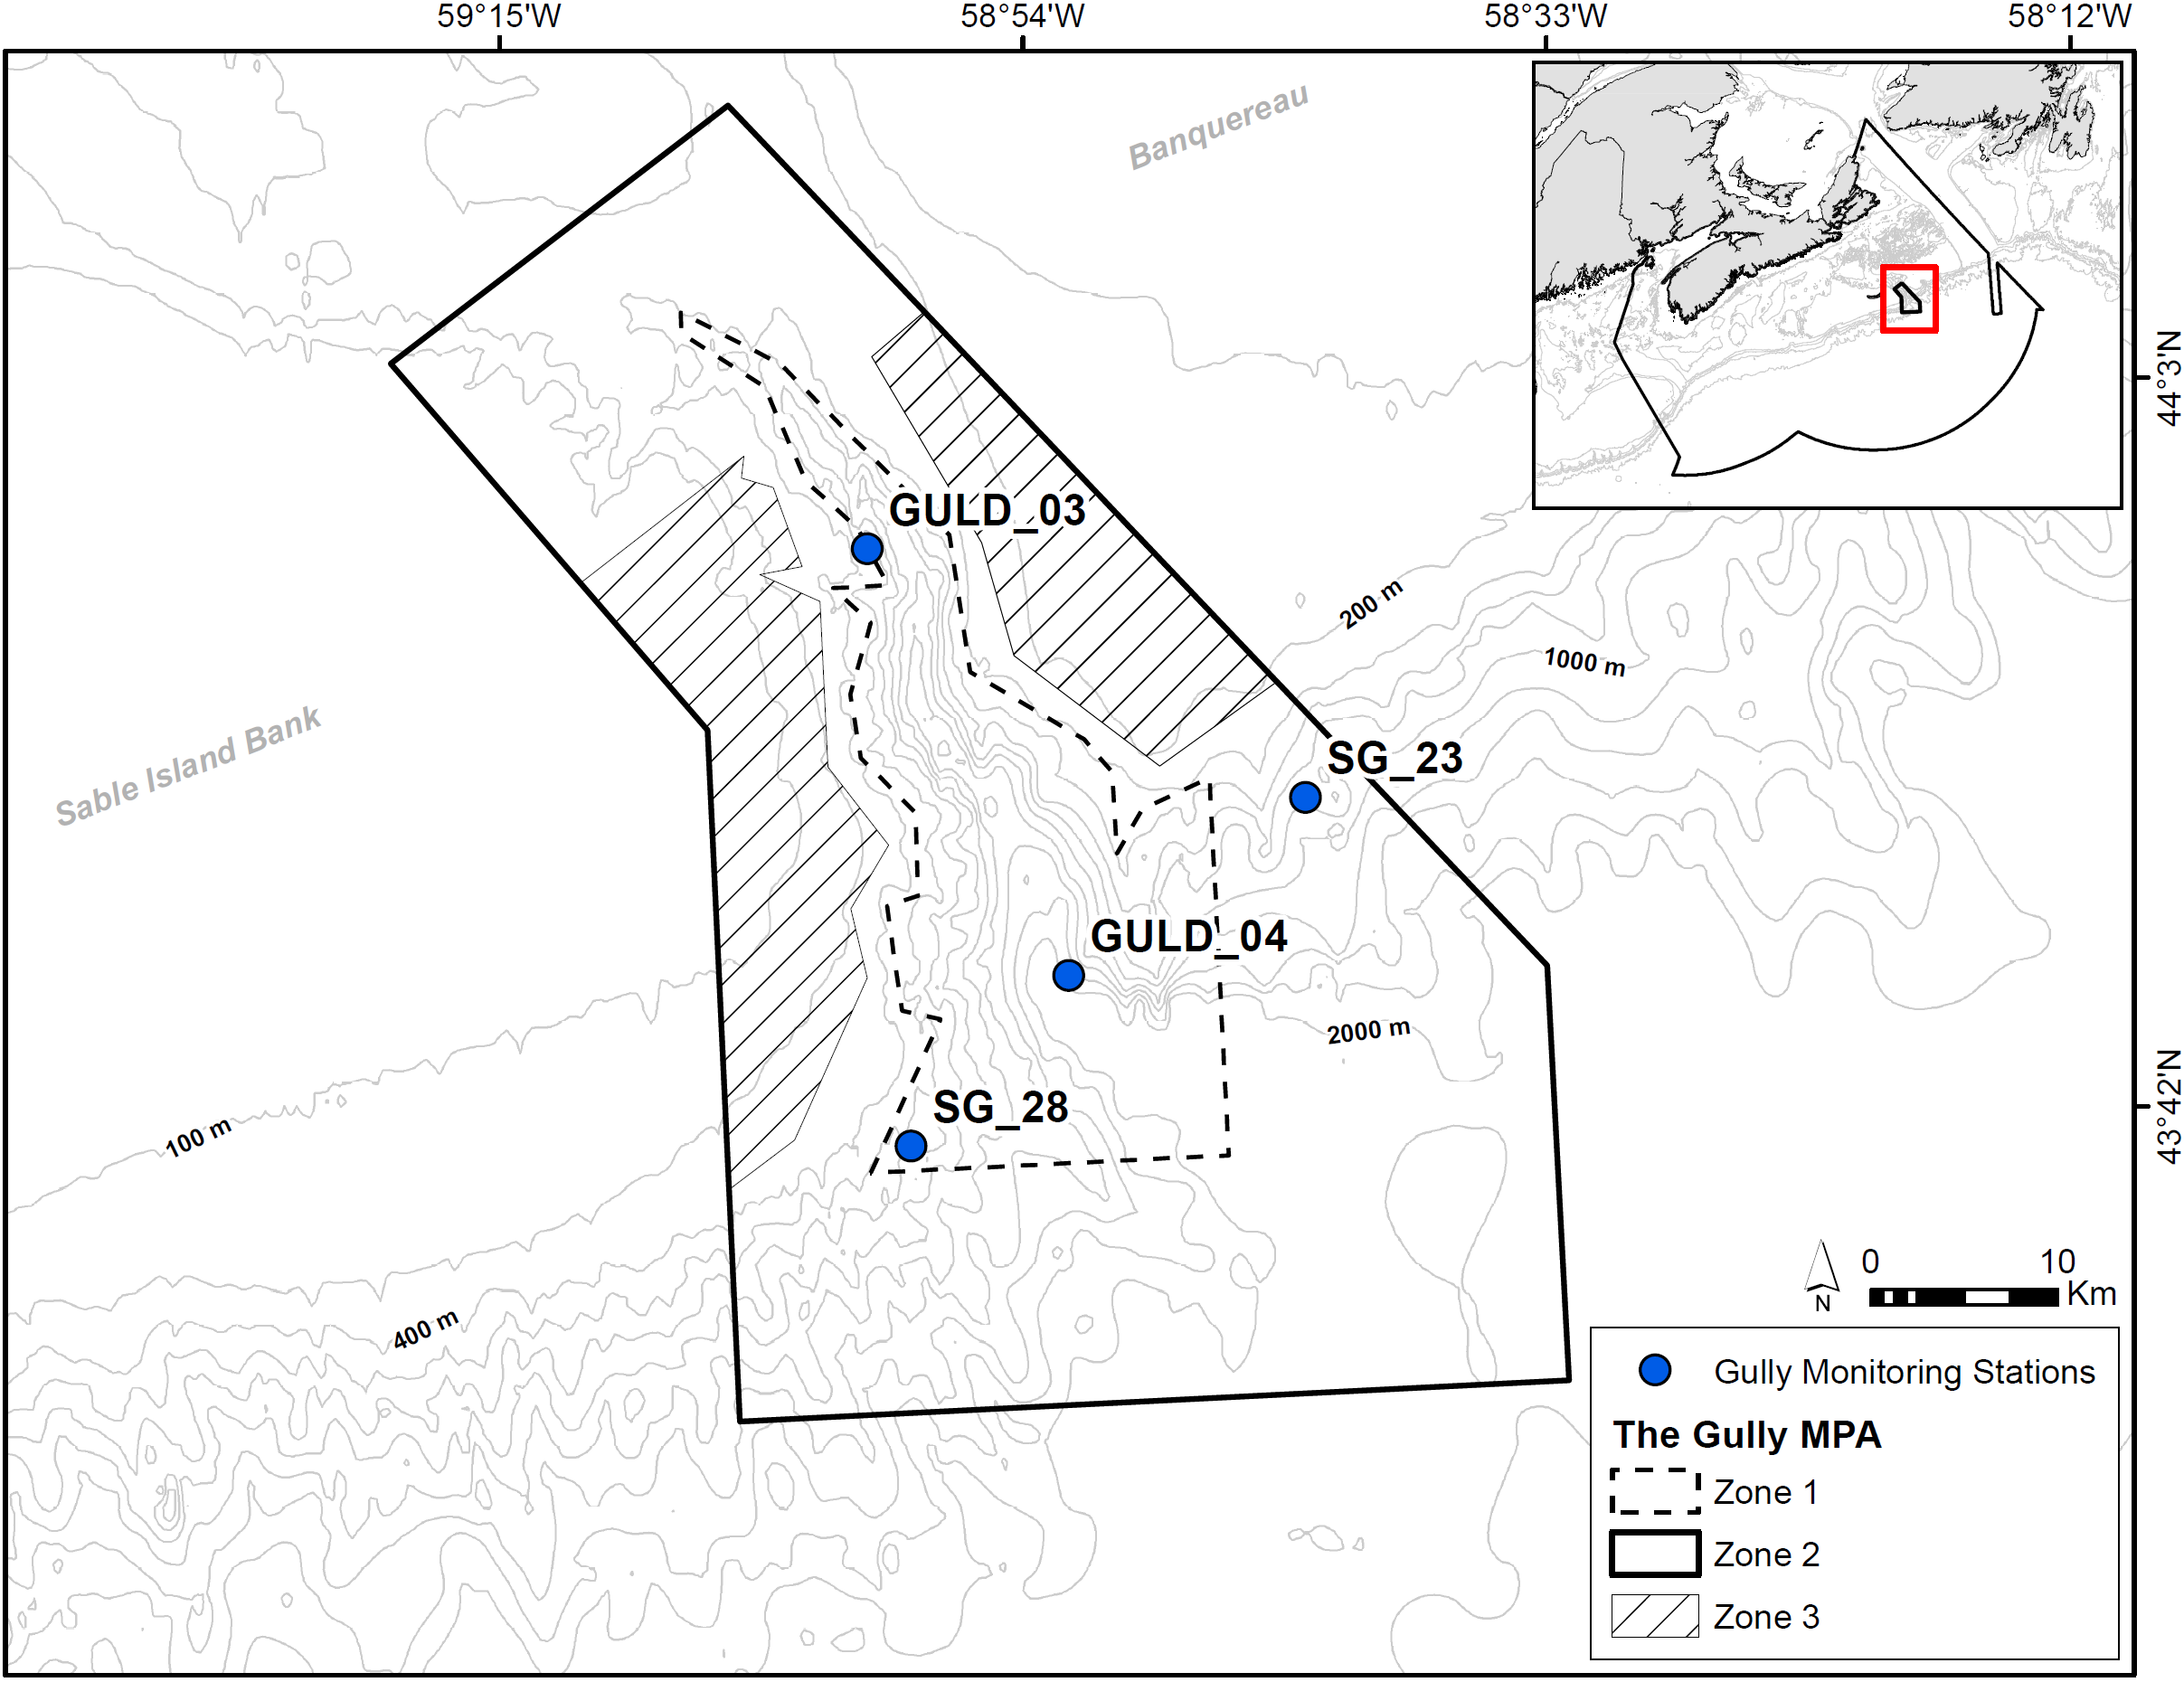
\includegraphics[width=6in]{figure/Figure01}}{Figure \ref{fig:figure1}} 

}

\caption{Location of the four AZMP fixed stations in the Gully MPA (blue circles). The boundaries of the three Gully Management Zones are also shown. Top-right map inset shows the position of the Gully MPA in relation to Atlantic Canada and DFO's Maritime Region administrative boundary.}\label{fig:figure1}
\end{figure}
\vspace*{\fill}

\clearpage


\begin{figure}[htb]

{\centering \pdftooltip{\includegraphics[width=6in]{figure/Figure02}}{Figure \ref{fig:figure2}} 

}

\caption{Location of the four AZMP fixed monitoring stations in the Gully MPA in relation to canyon topography as highlighted by 15 m resolution multibeam bathymetry. The nominal location of each station is represented by the blue circles, while all occupations where CTD data were collected and considered in this report are represented by fuchsia circles.}\label{fig:figure2}
\end{figure}
\clearpage


\begin{figure}[htb]

{\centering \pdftooltip{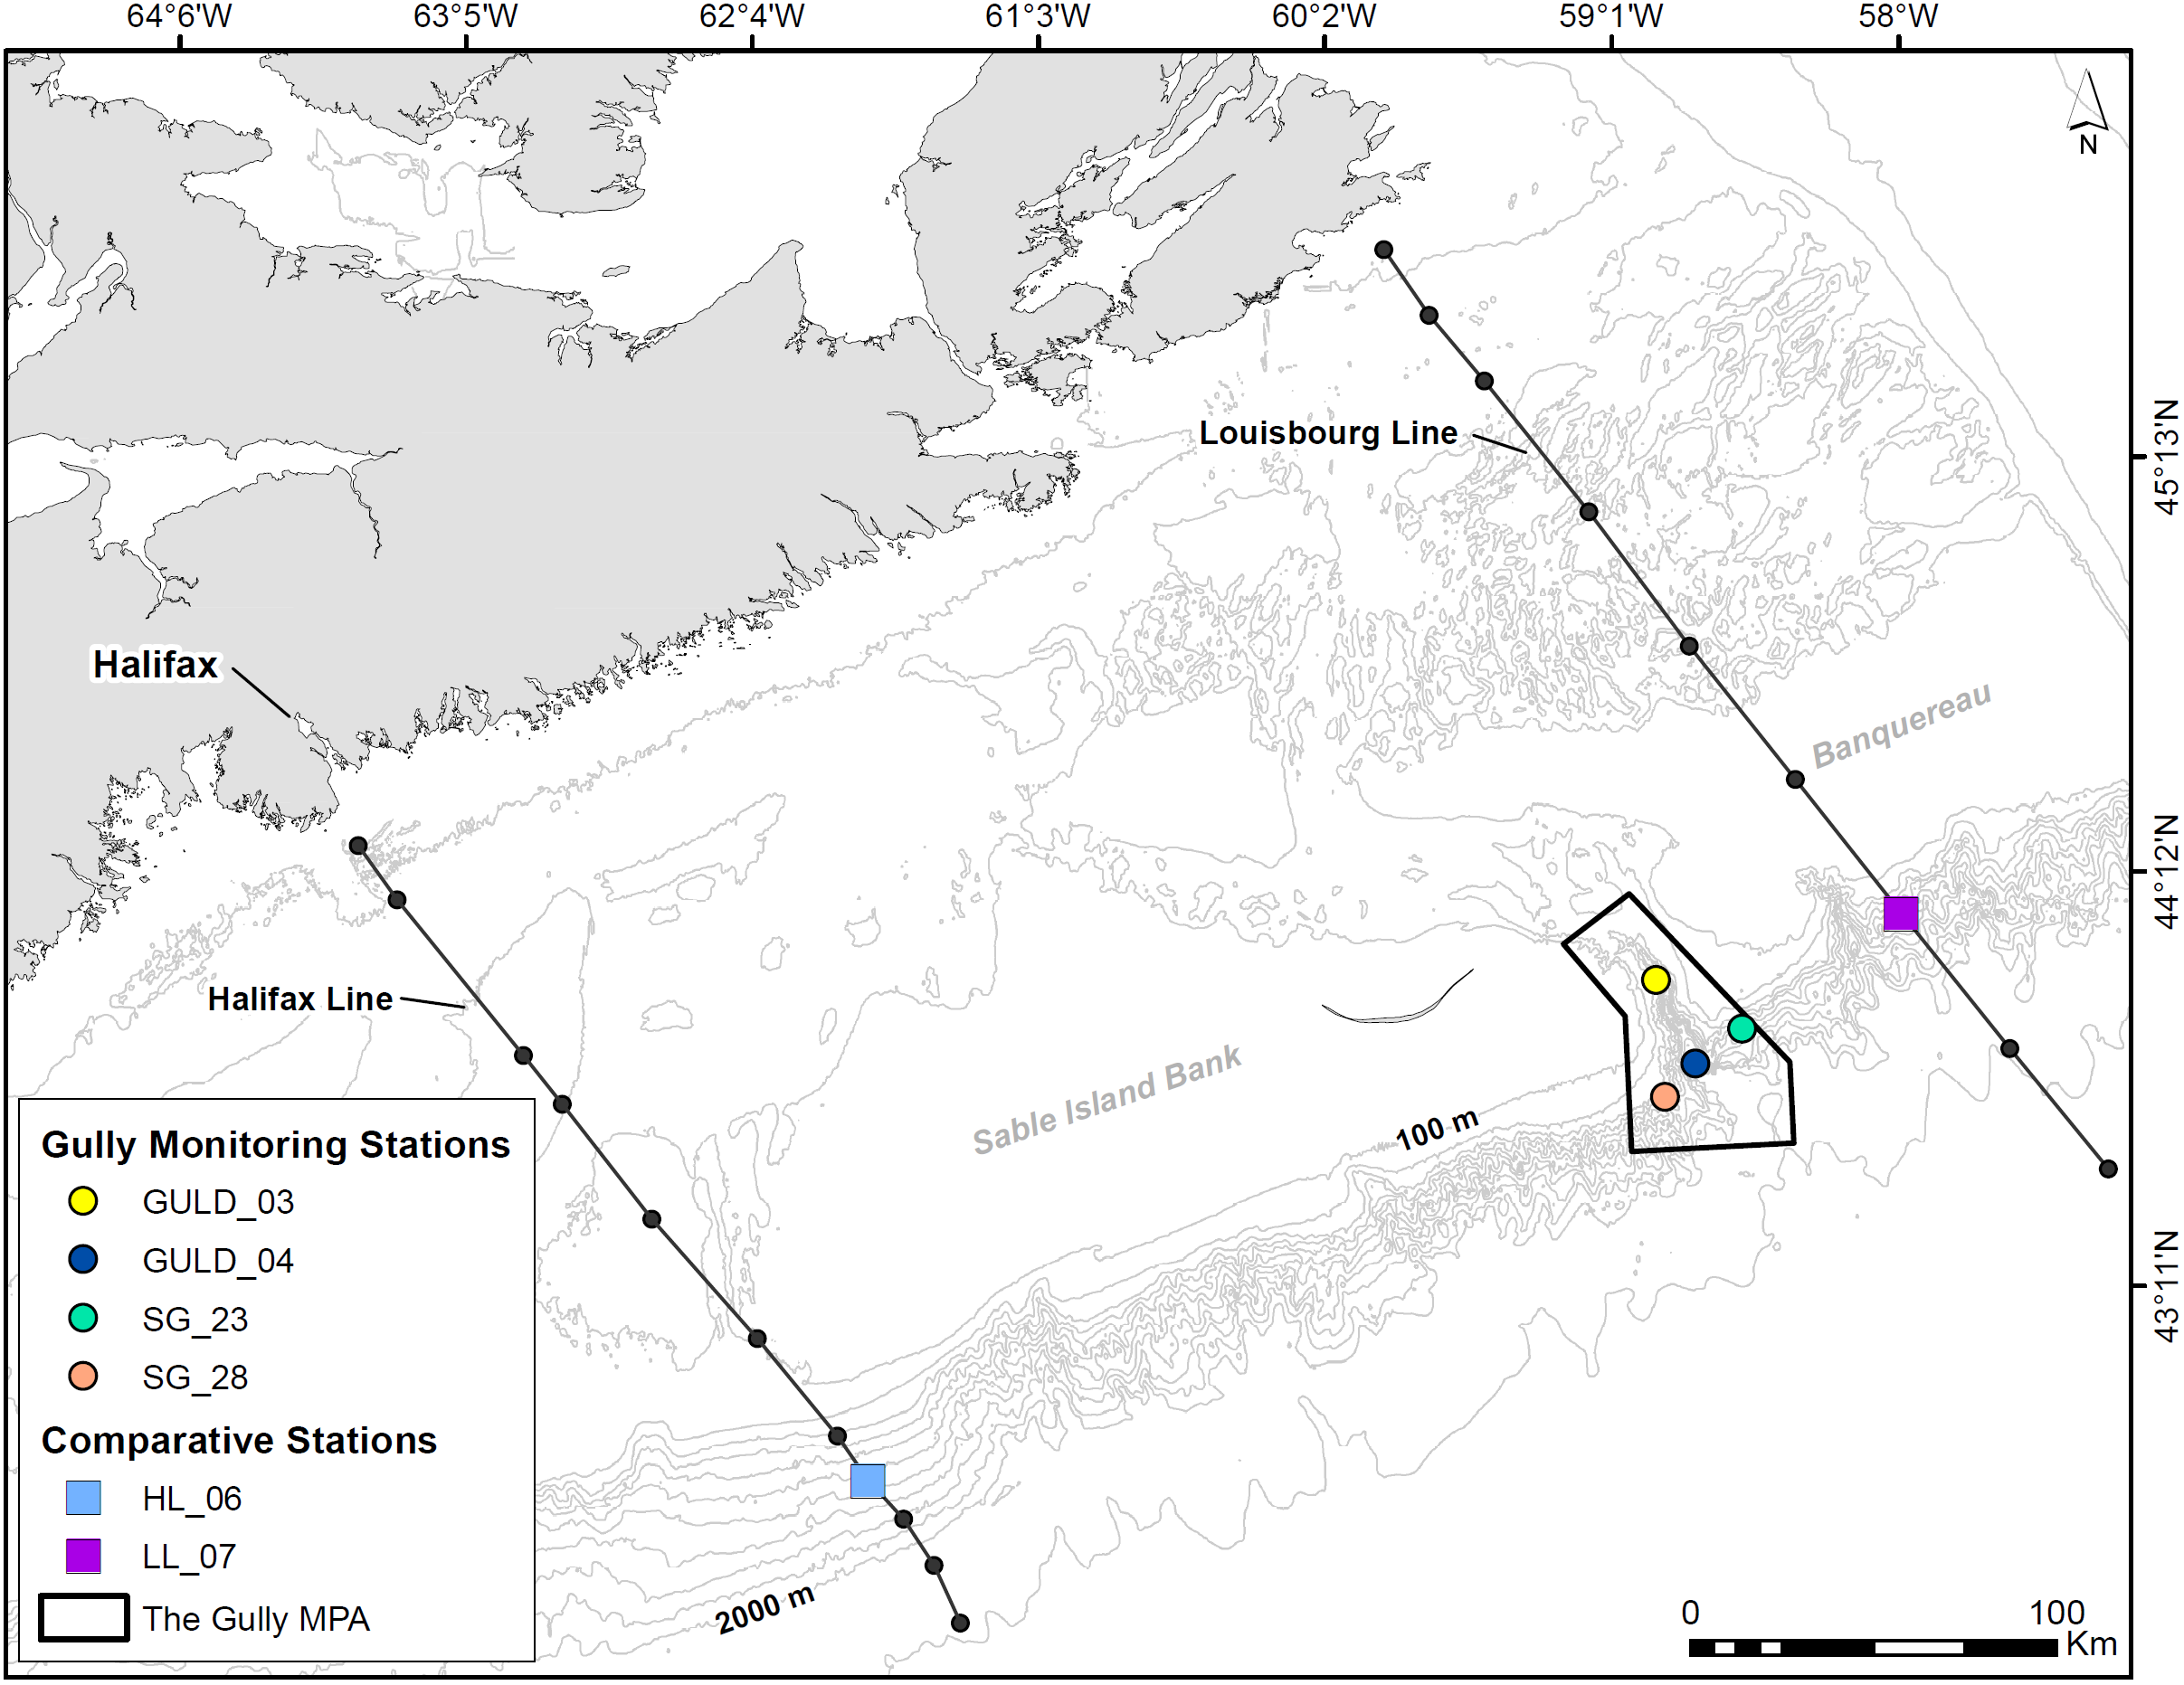
\includegraphics[width=6in]{figure/Figure03}}{Figure \ref{fig:figure3}} 

}

\caption{The Gully MPA in relation to comparative upstream (LL\_07) and downstream (HL\_06) stations from the AZMP's core Louisbourg and Halifax lines, respectively.}\label{fig:figure3}
\end{figure}
\clearpage


\begin{figure}[htb]

{\centering \pdftooltip{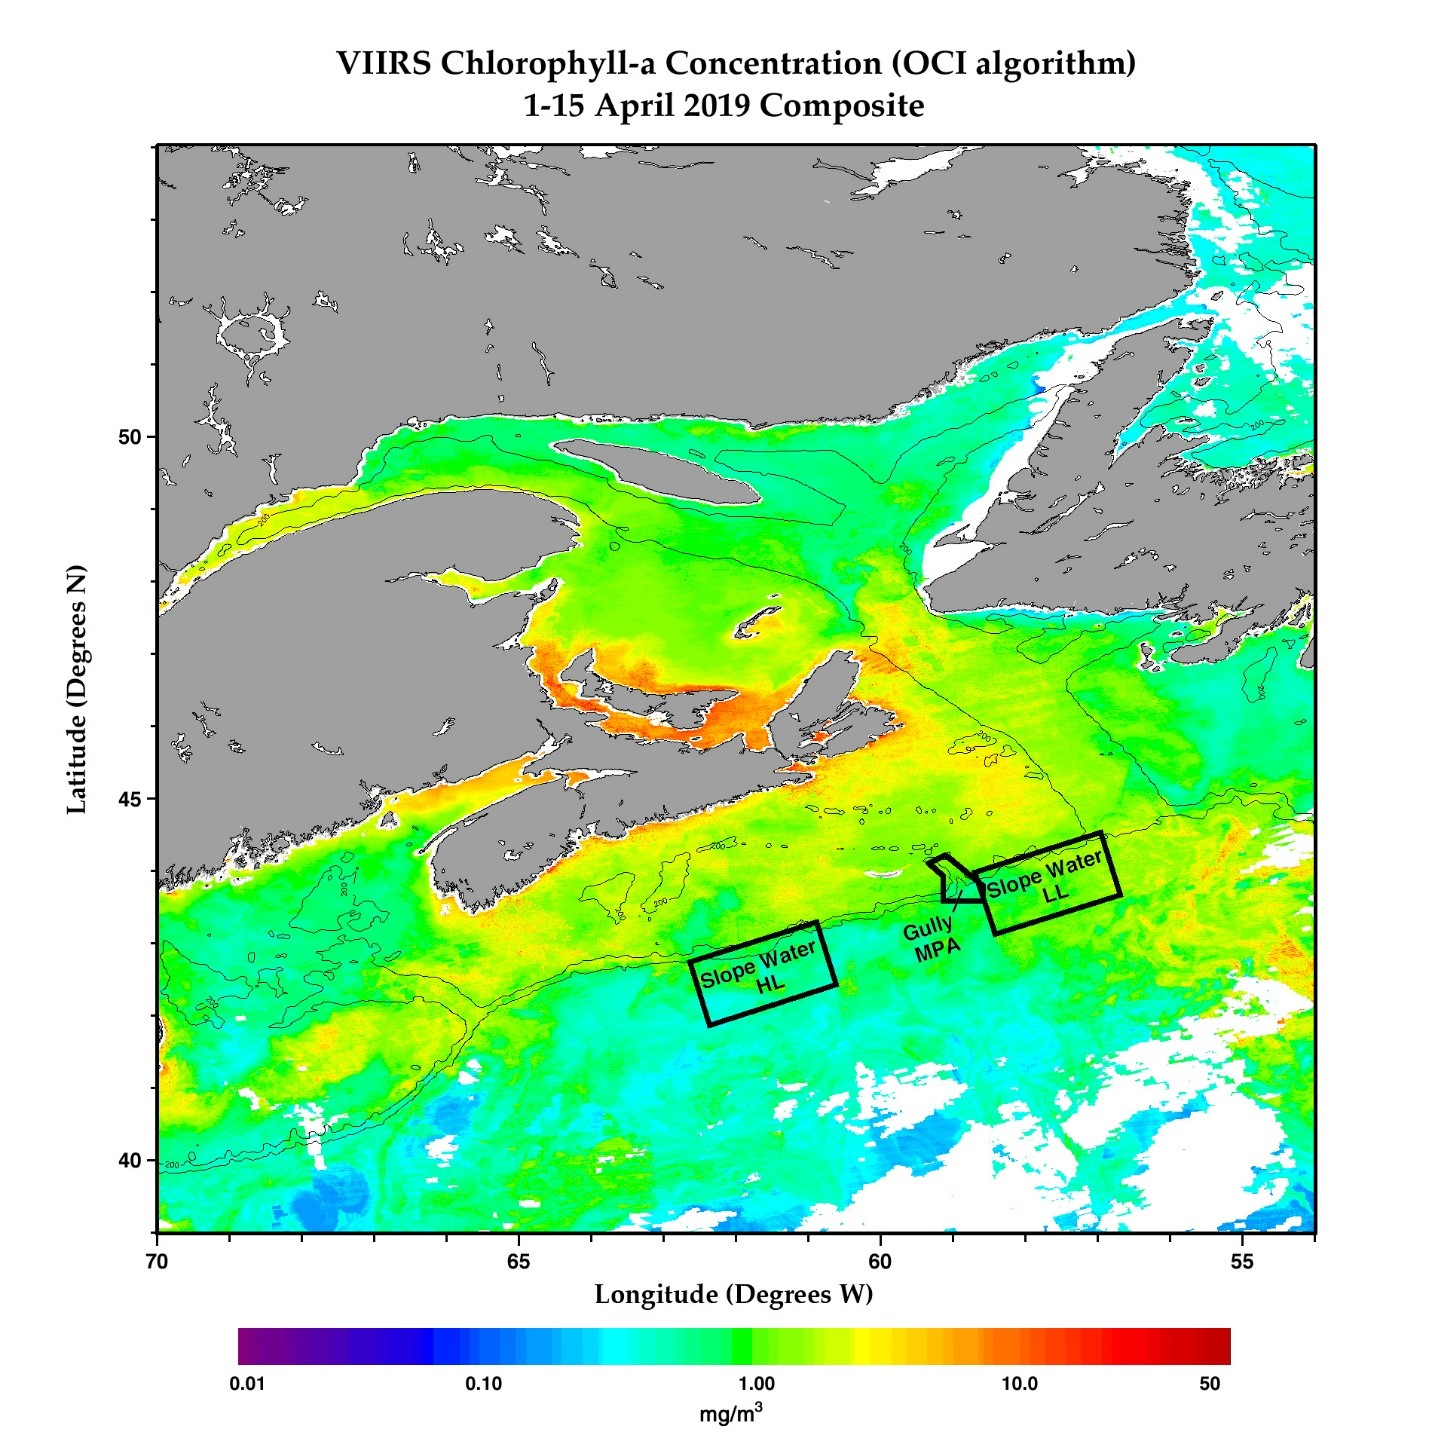
\includegraphics[width=6in]{figure/Figure04}}{Figure \ref{fig:figure4}} 

}

\caption{Areas of the slope waters upstream (Slope Water LL) and downstream (Slope Water HL) of the Gully MPA for which bi-weekly satellite measurements of Sea Surface Temperature (SST) and Sea Surface Chlorophyll (SSC) were calculated between 1998 and 2018.}\label{fig:figure4}
\end{figure}
\clearpage


\begin{landscapepage}
\begin{figure}[htb]

{\centering \pdftooltip{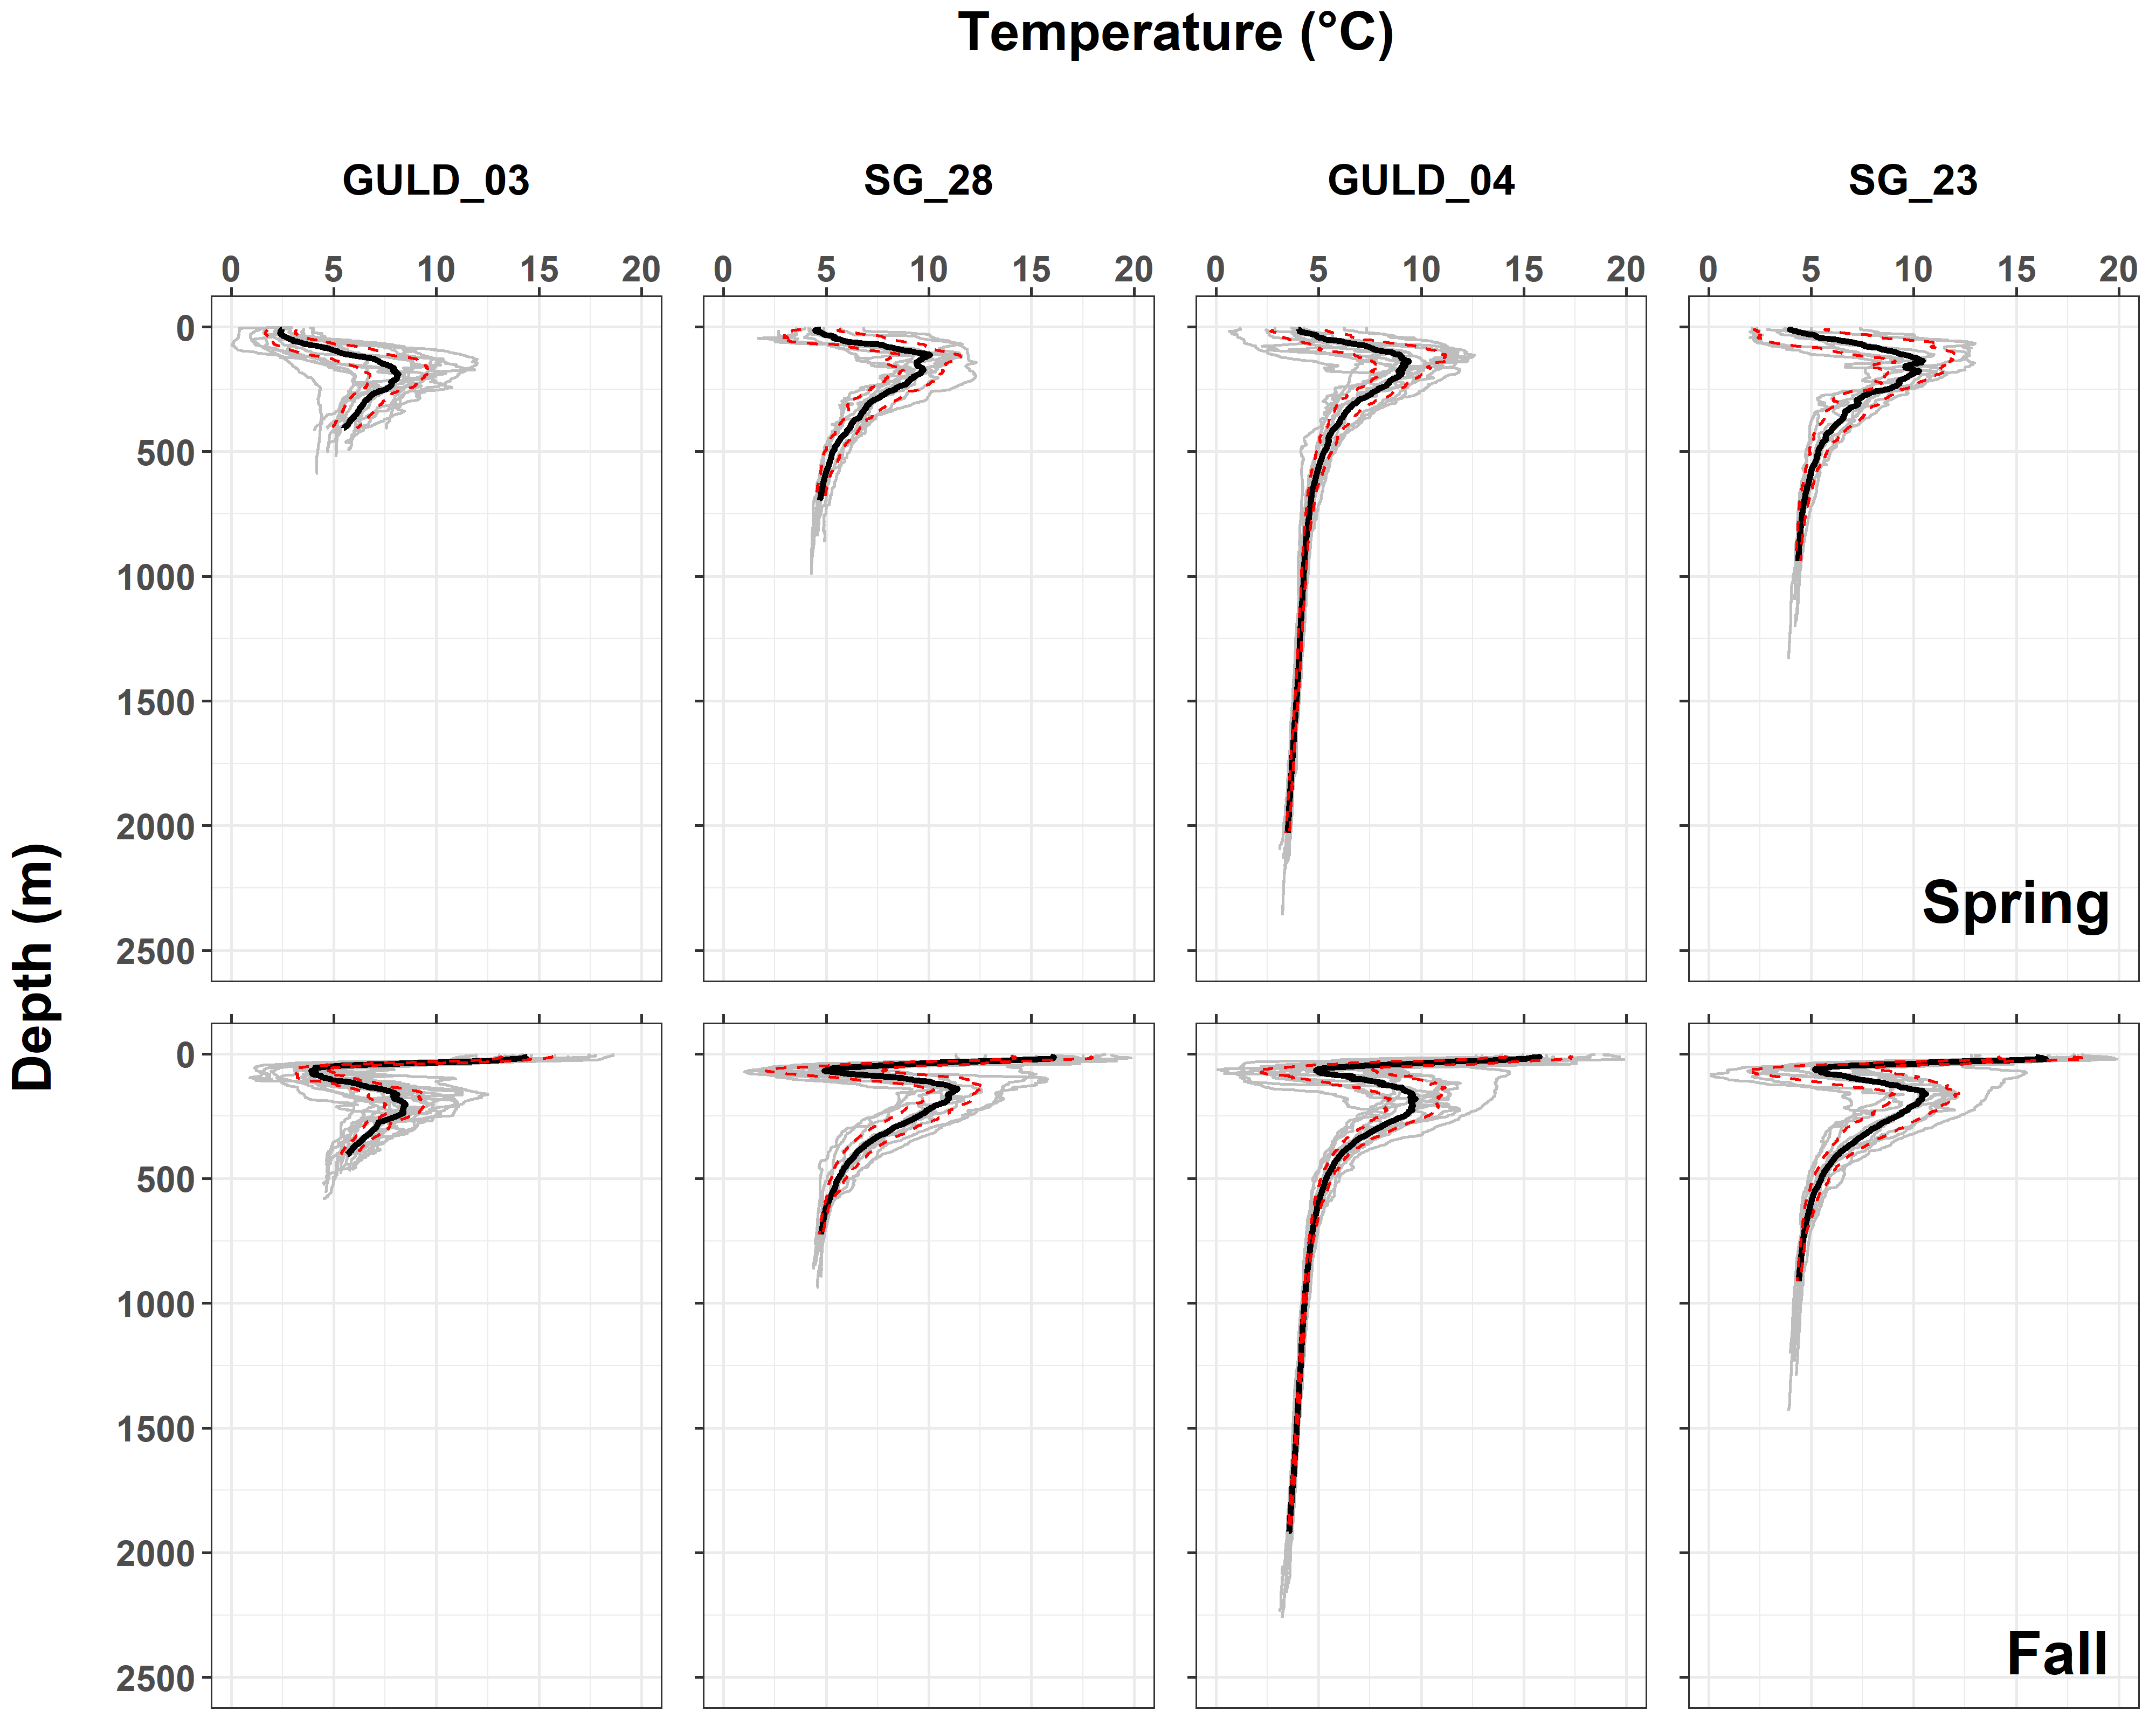
\includegraphics[width=7.5in]{figure/Figure05}}{Figure \ref{fig:figure5}} 

}

\caption{Mean (black line) temperature (\(\degree\)C) \thickspace \(\pm\) \thinspace 95\% confidence interval (red dash) calculated across individual CTD profiles (grey lines) collected at each of the four AZMP fixed stations in the Gully during the spring (top panel: April) and fall (bottom panel: September and October). Mean conditions at each station were computed by averaging the values in each 1 m depth bin across casts collected within each season.}\label{fig:figure5}
\end{figure}
\end{landscapepage}
\clearpage


\begin{landscapepage}
\begin{figure}[htb]

{\centering \pdftooltip{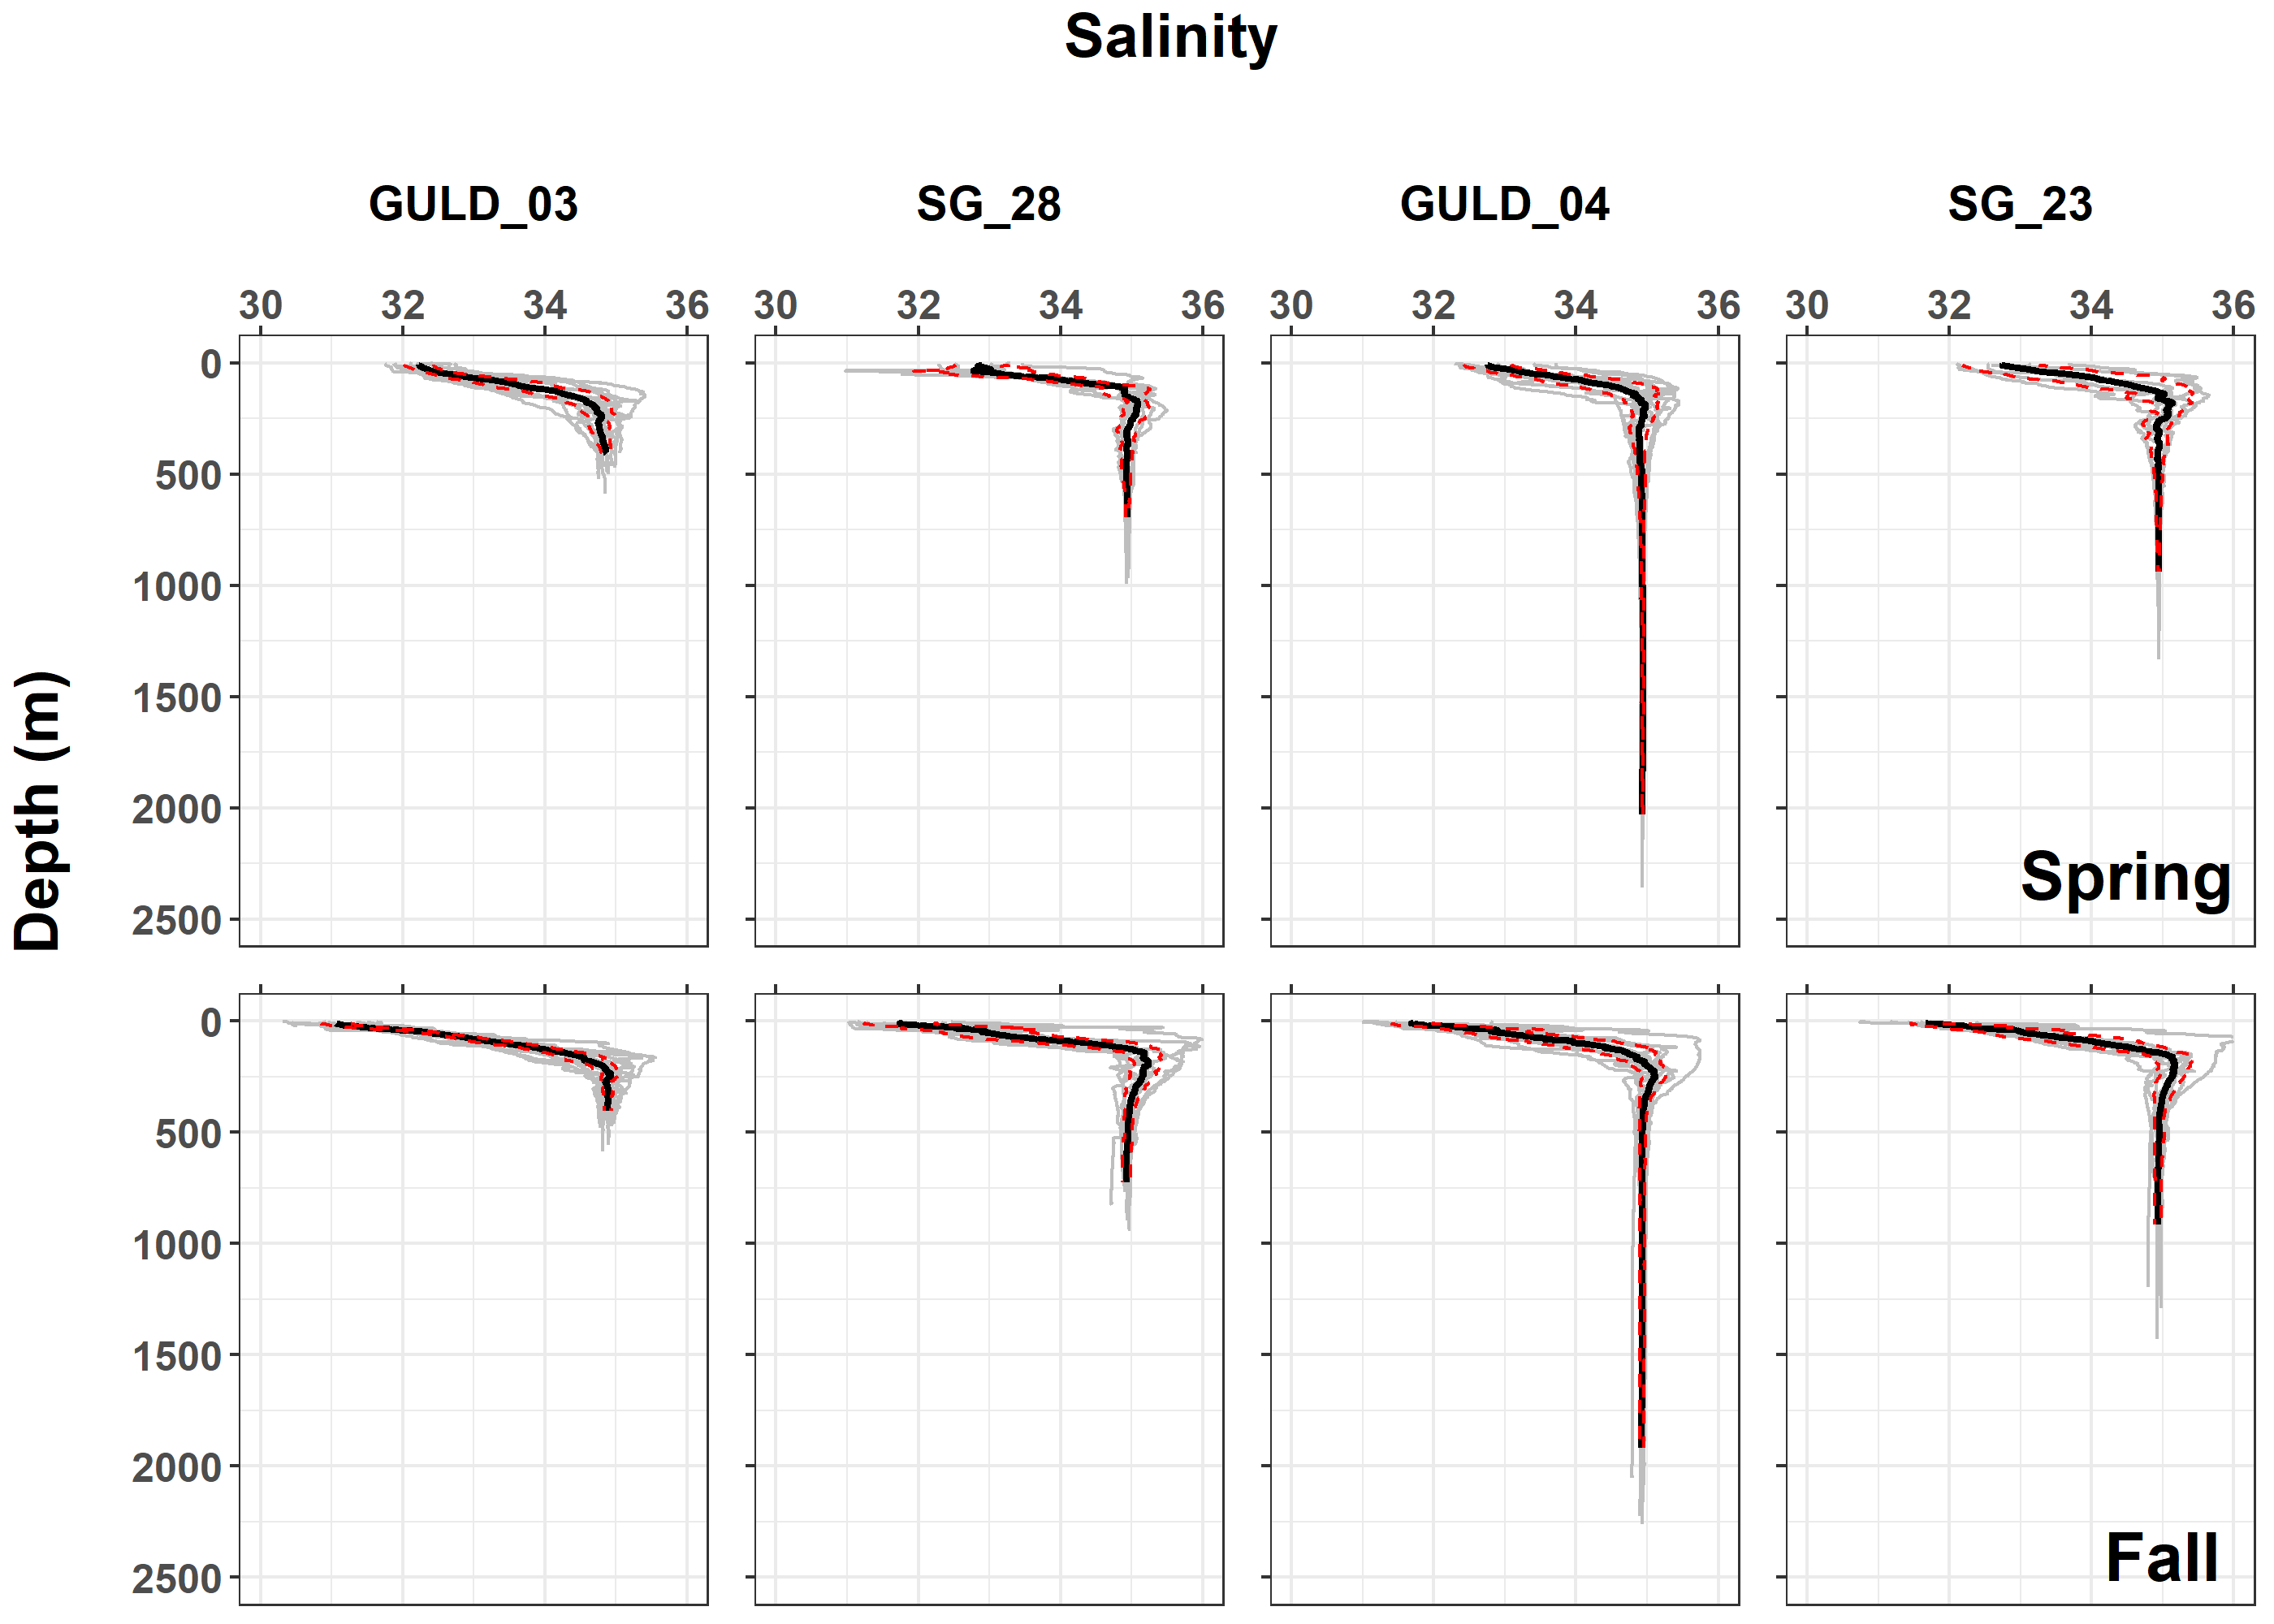
\includegraphics[width=7.5in]{figure/Figure06}}{Figure \ref{fig:figure6}} 

}

\caption{Mean (black line) salinity \(\pm\) 95\% confidence interval (red dash) calculated across individual CTD profiles (grey lines) collected at each of the four AZMP fixed stations in the Gully during the spring (April; top panel) and fall (September and October; bottom panel). Mean conditions at each station were computed by averaging the values in each 1 depth bin across casts collected within each season.}\label{fig:figure6}
\end{figure}
\end{landscapepage}
\clearpage


\begin{landscapepage}
\begin{figure}[htb]

{\centering \pdftooltip{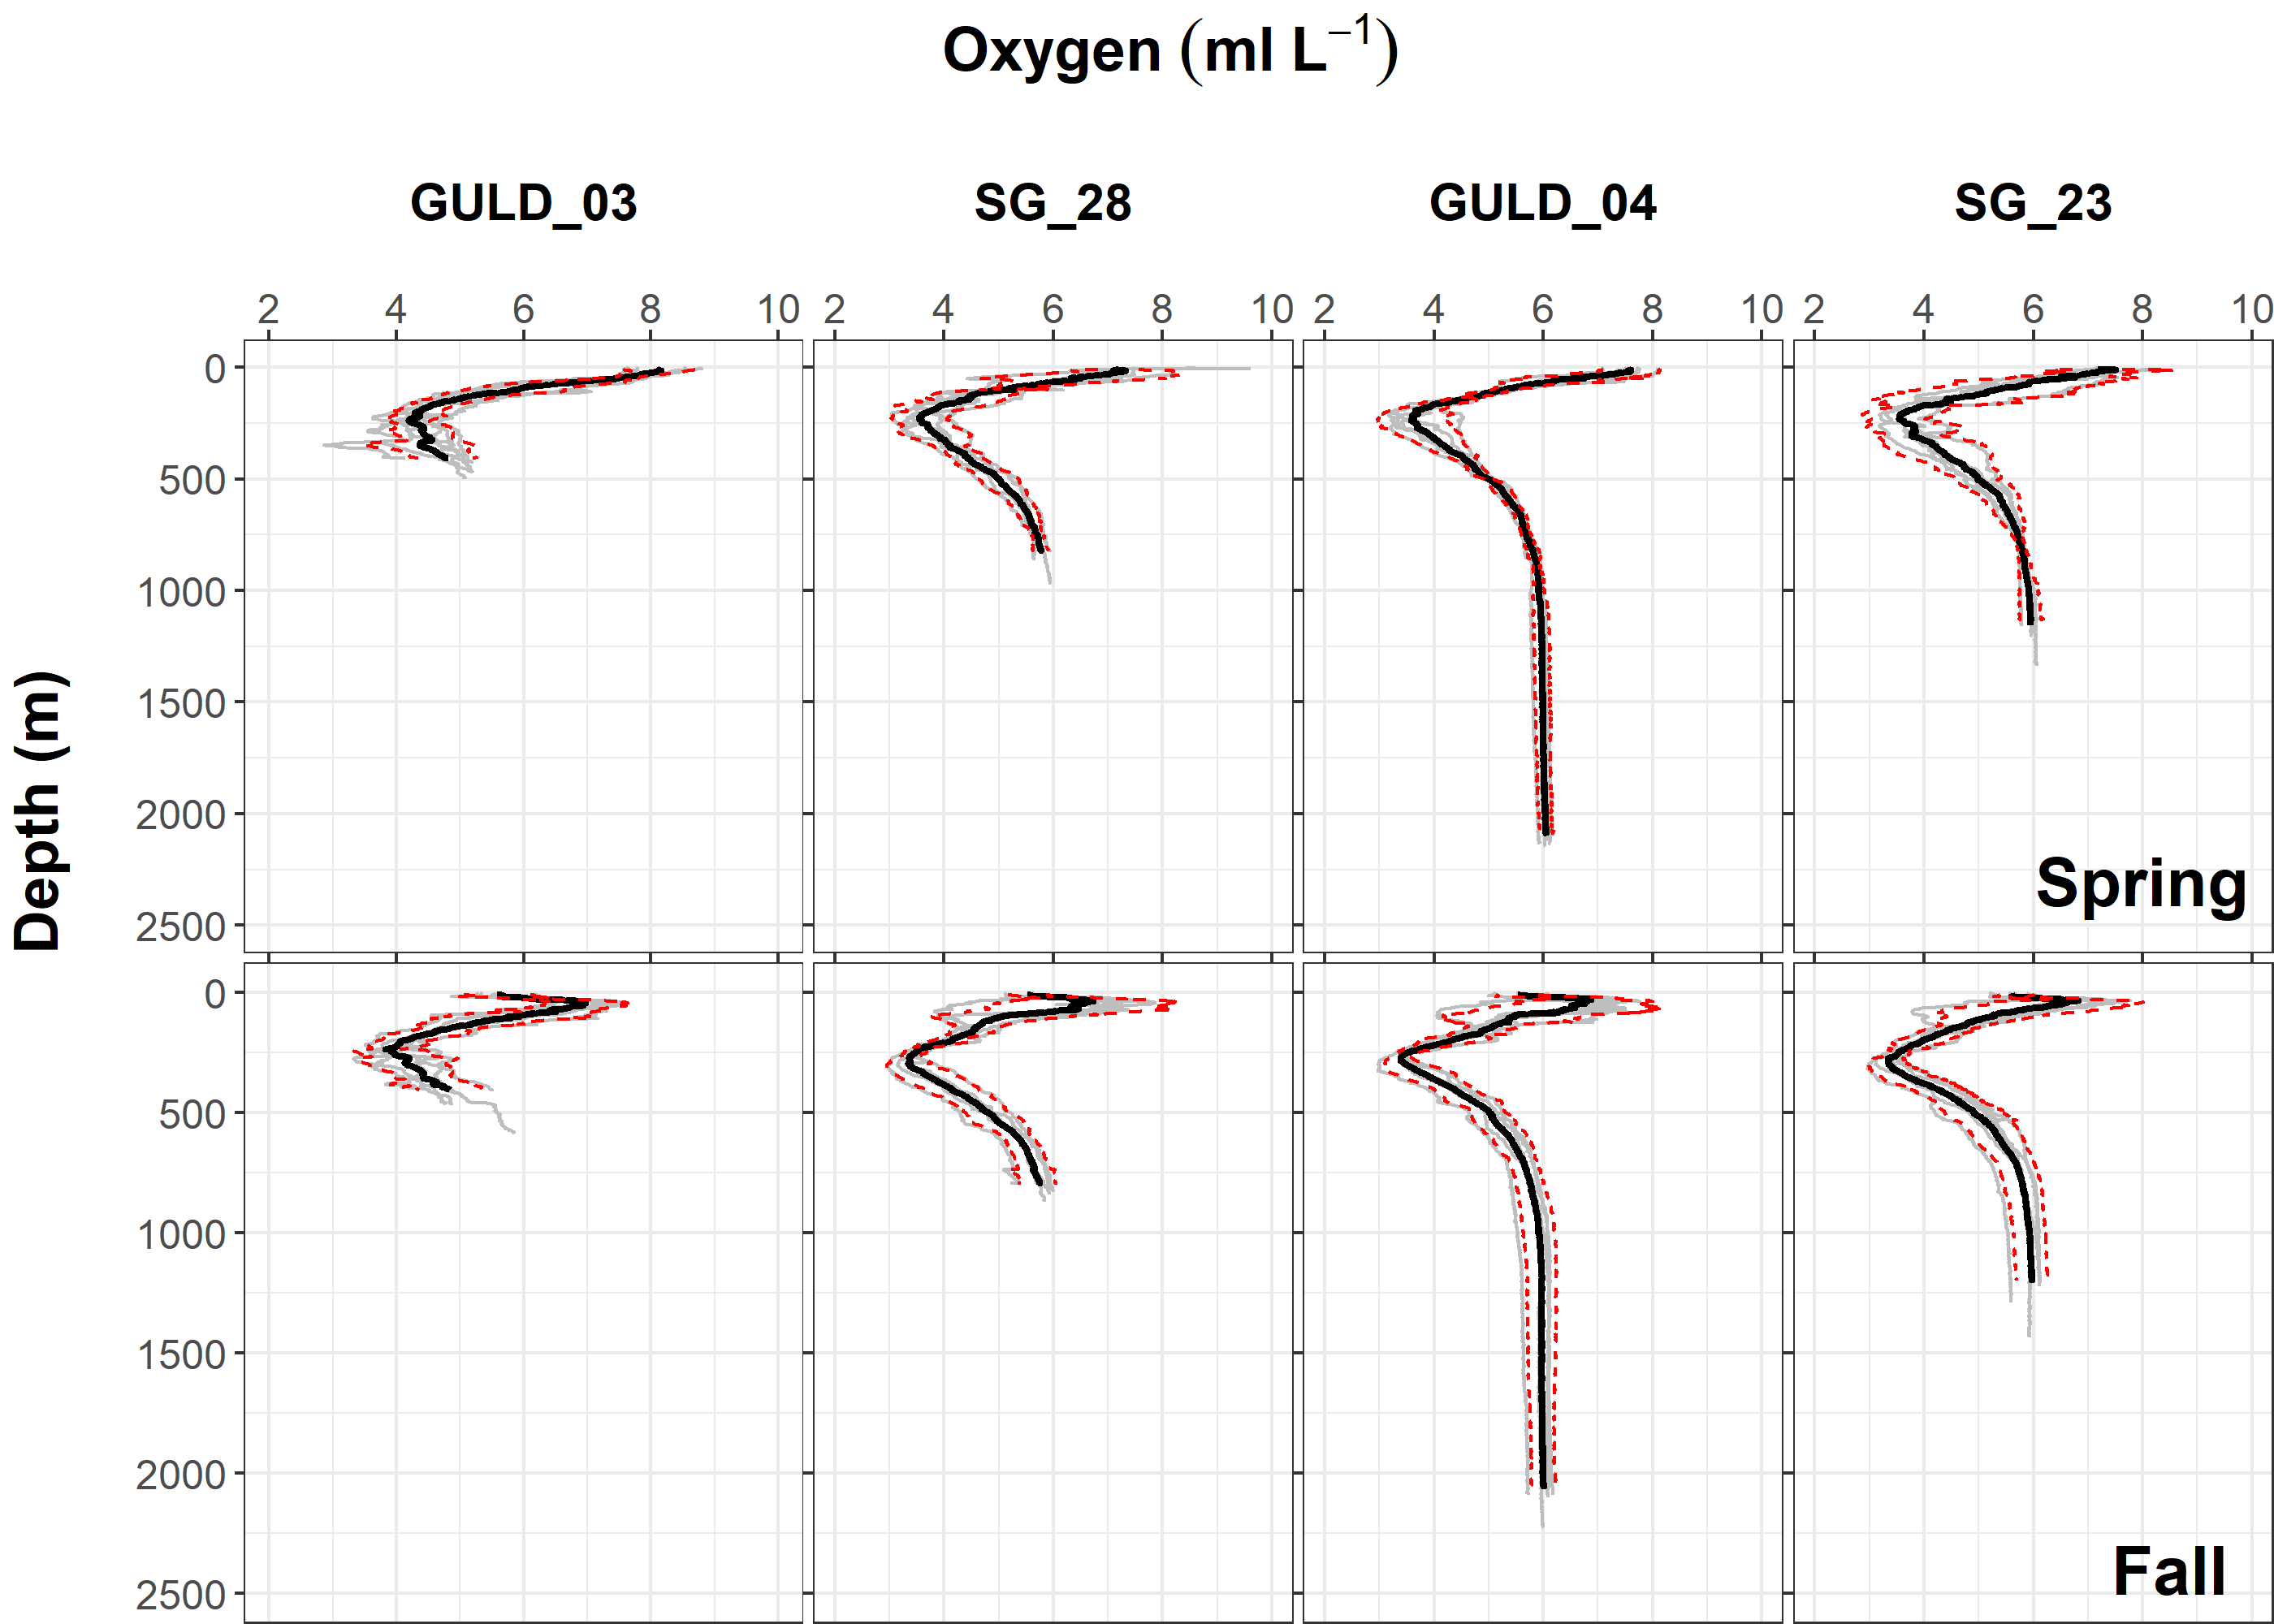
\includegraphics[width=7.5in]{figure/Figure07}}{Figure \ref{fig:figure7}} 

}

\caption{Mean (black line) oxygen (ml L\textsuperscript{-1}) \(\pm\) 95\% confidence interval (red dash) calculated across individual CTD profiles (grey lines) collected at each of the four AZMP fixed stations in the Gully during the spring (April; top panel) and fall (September and October; bottom panel). Mean conditions at each station were computed by averaging the values in each 1 depth bin across casts collected within each season. Oxygen data presented for each station is from 2013 onward.}\label{fig:figure7}
\end{figure}
\end{landscapepage}
\clearpage


\begin{landscapepage}
\begin{figure}[htb]

{\centering \pdftooltip{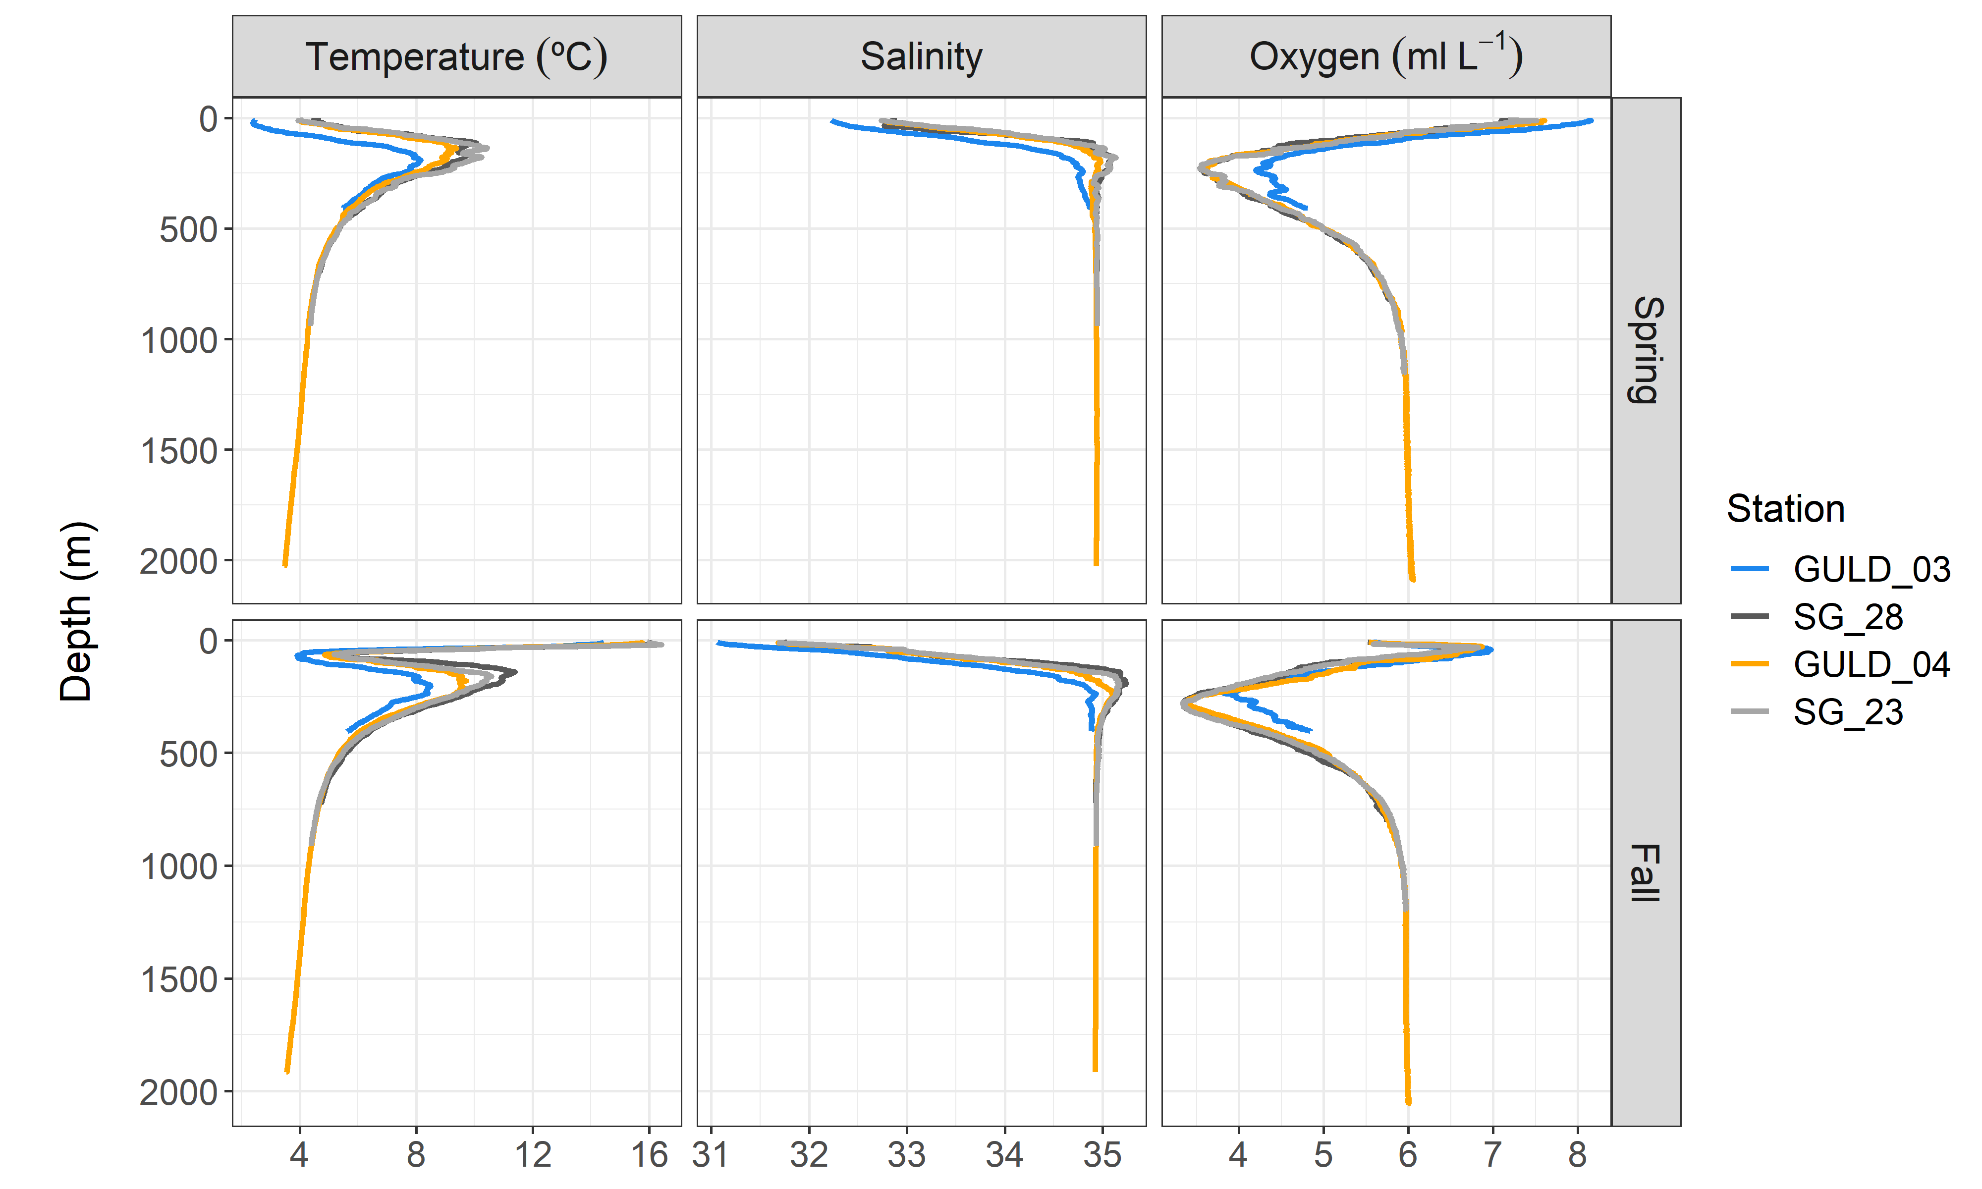
\includegraphics[width=9.25in]{figure/Figure08}}{Figure \ref{fig:figure8}} 

}

\caption{Comparison of the vertically-averaged temperature (\(\degree\)C), salinity, and dissolved oxygen (ml L\textsuperscript{-1}) profiles at each of the four AZMP fixed stations in the Gully during spring (April) and fall (September and October). Data were collected between 2000 to 2018 for GULD\_03 and GULD\_04, and 2007 to 2018 for SG\_23 and SG\_28 (with slight variations between seasons). Oxygen data presented for each station is from 2013 onward.}\label{fig:figure8}
\end{figure}
\end{landscapepage}
\clearpage


\begin{landscapepage}
\begin{figure}[htb]

{\centering \pdftooltip{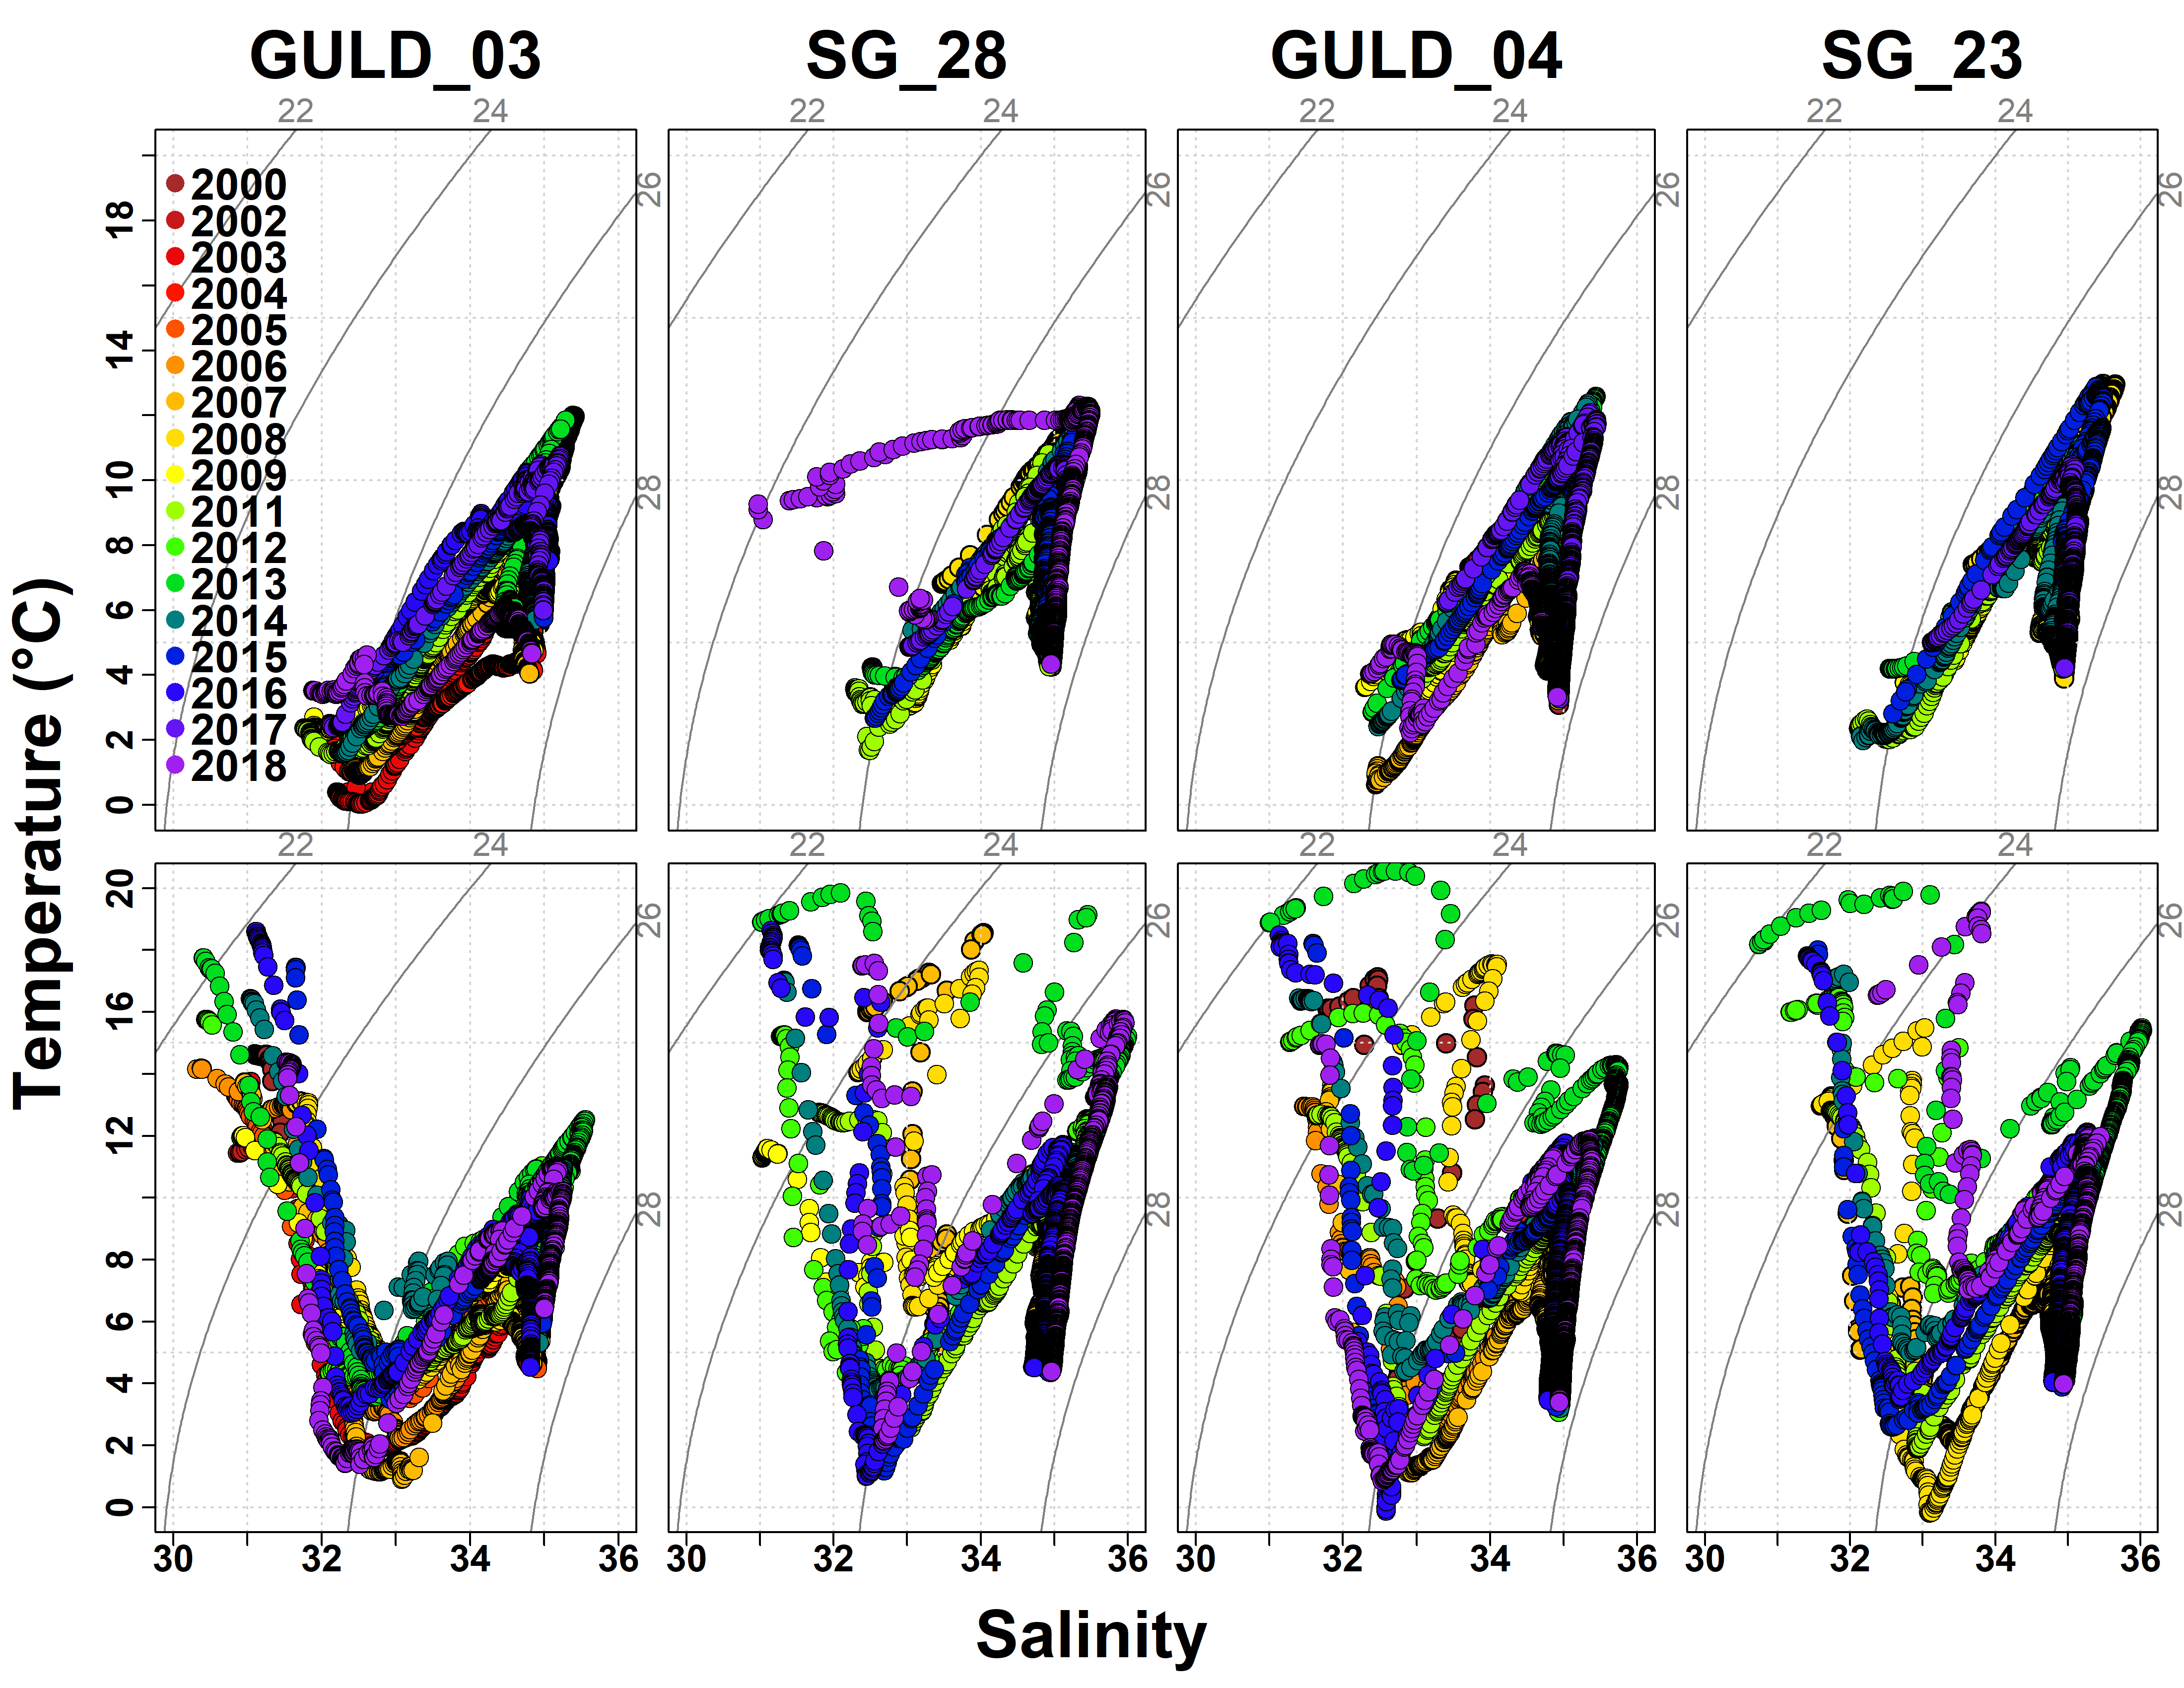
\includegraphics[width=9.0in]{figure/Figure09}}{Figure \ref{fig:figure9}} 

}

\caption{Temperature-Salinity (T-S) plots of CTD profile data collected at each of the four AZMP fixed stations in the Gully in during the spring (April; top panel) and fall (September and October; bottom panel). Data were collected between 2000 to 2018 for GULD\_03 and GULD\_04, and 2007 to 2018 for SG\_23 and SG\_28 (with slight variations between seasons).}\label{fig:figure9}
\end{figure}
\end{landscapepage}
\clearpage


\begin{figure}[htb]

{\centering \pdftooltip{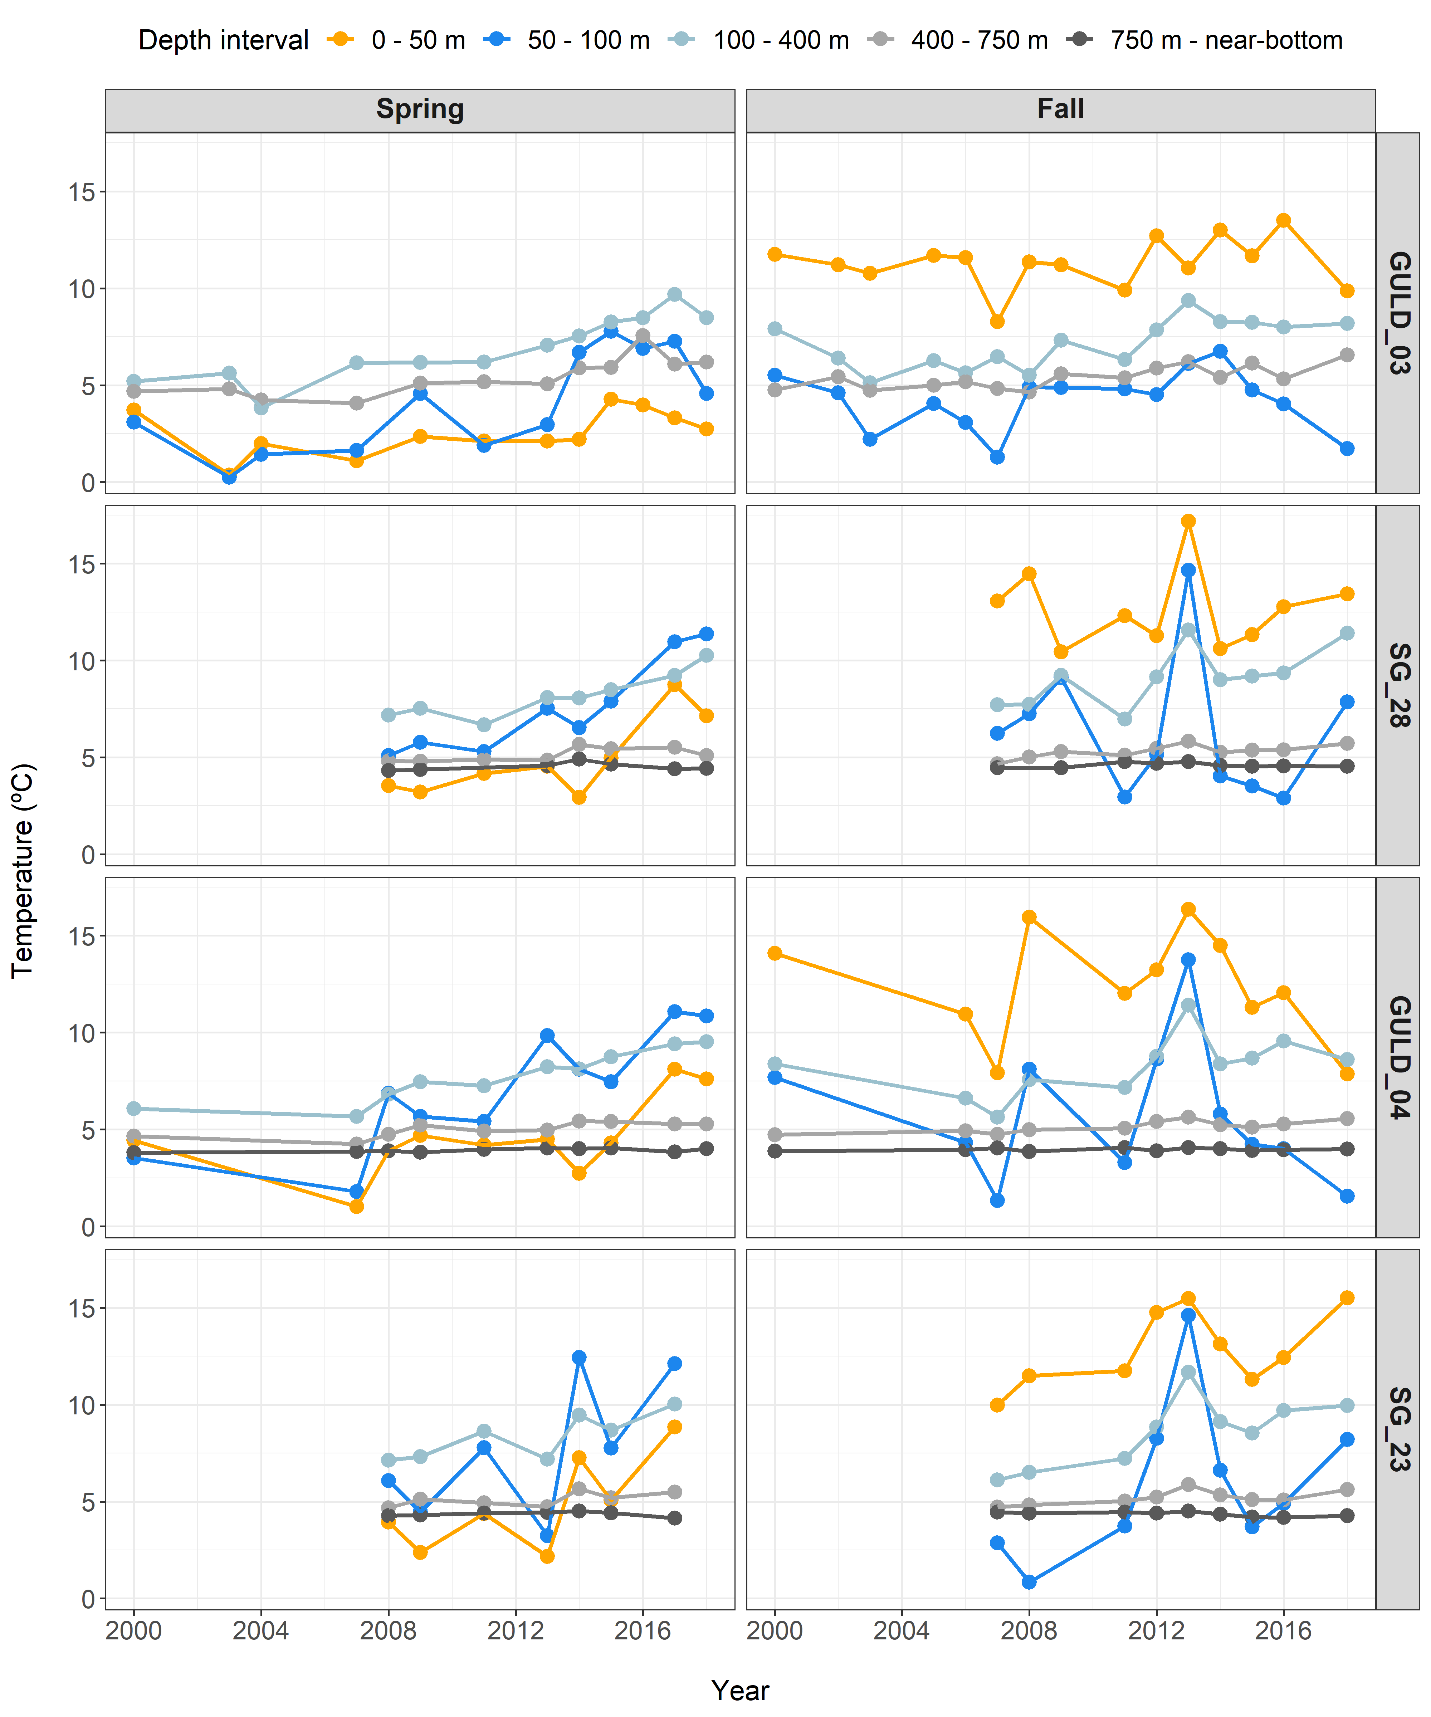
\includegraphics[width=6in]{figure/Figure10}}{Figure \ref{fig:figure10}} 

}

\caption{Changes in mean spring and fall temperature (\(\degree\)C) in five vertical depth intervals sampled at each of the four AZMP fixed stations in the Gully. Circles represent mean temperature at each depth interval and year. Absent circles indicate that sampling did not occur at that station in that year. Date range of data collection varies between stations and is summarized in Table~\ref{tab:table2}. Note that the 400 to 750 m depth interval for GULD\_03 spans from \textgreater400 to near-bottom (up to 586 m).}\label{fig:figure10}
\end{figure}
\clearpage


\begin{figure}[htb]

{\centering \pdftooltip{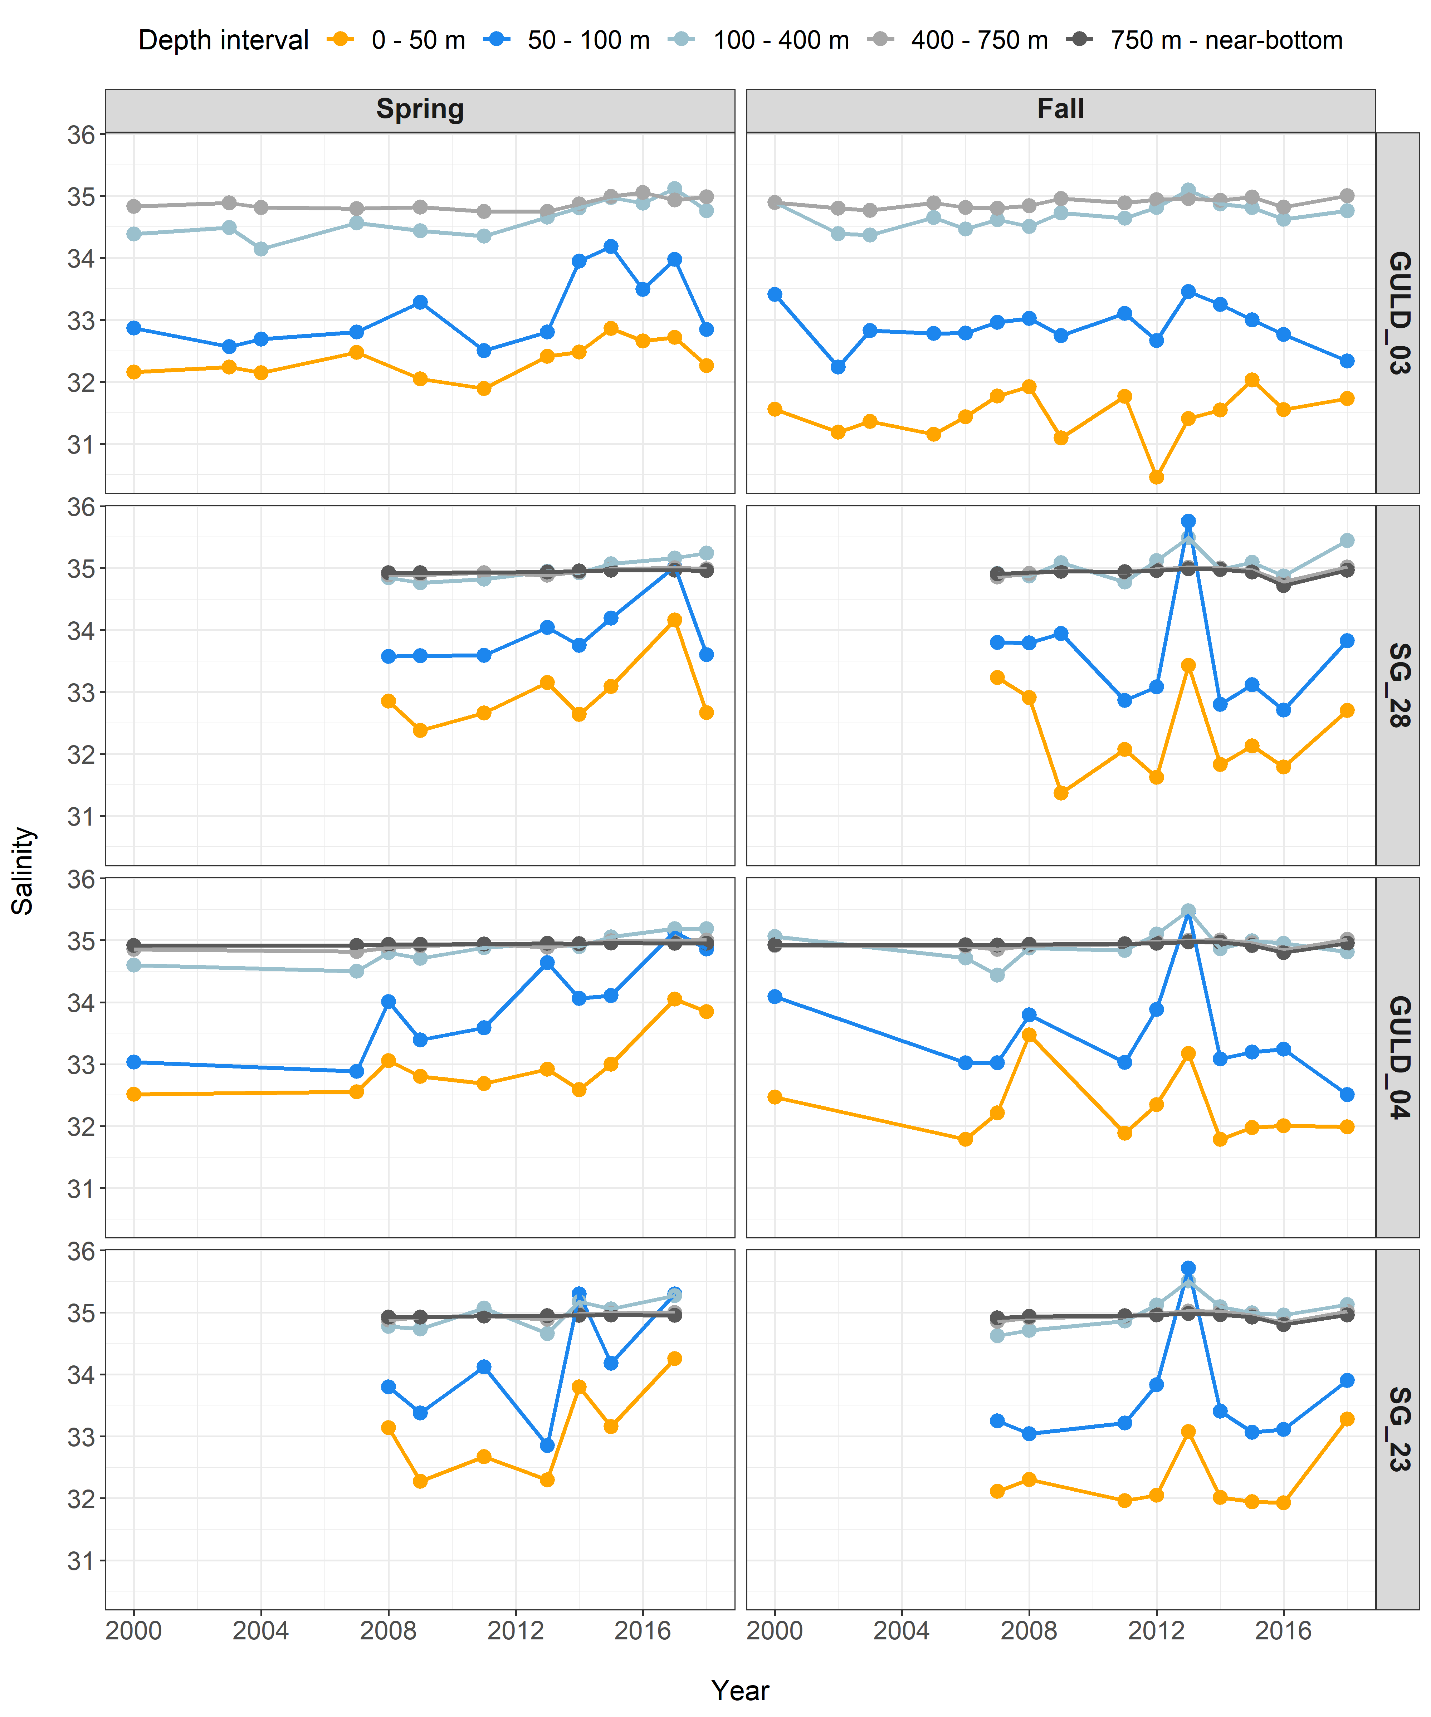
\includegraphics[width=6in]{figure/Figure11}}{Figure \ref{fig:figure11}} 

}

\caption{Changes in mean spring and fall salinity in five vertical depth intervals sampled at each of the four AZMP fixed stations in the Gully. Circles represent mean salinity at each depth interval and year. Absent circles indicate that sampling did not occur at that station in that year. Date range of data collection varies between stations and is summarized in Table~\ref{tab:table2}. Note that the 400 to 750 m depth interval for GULD\_03 spans from \textgreater400 to near-bottom (up to 586 m).}\label{fig:figure11}
\end{figure}
\clearpage


\begin{figure}[htb]

{\centering \pdftooltip{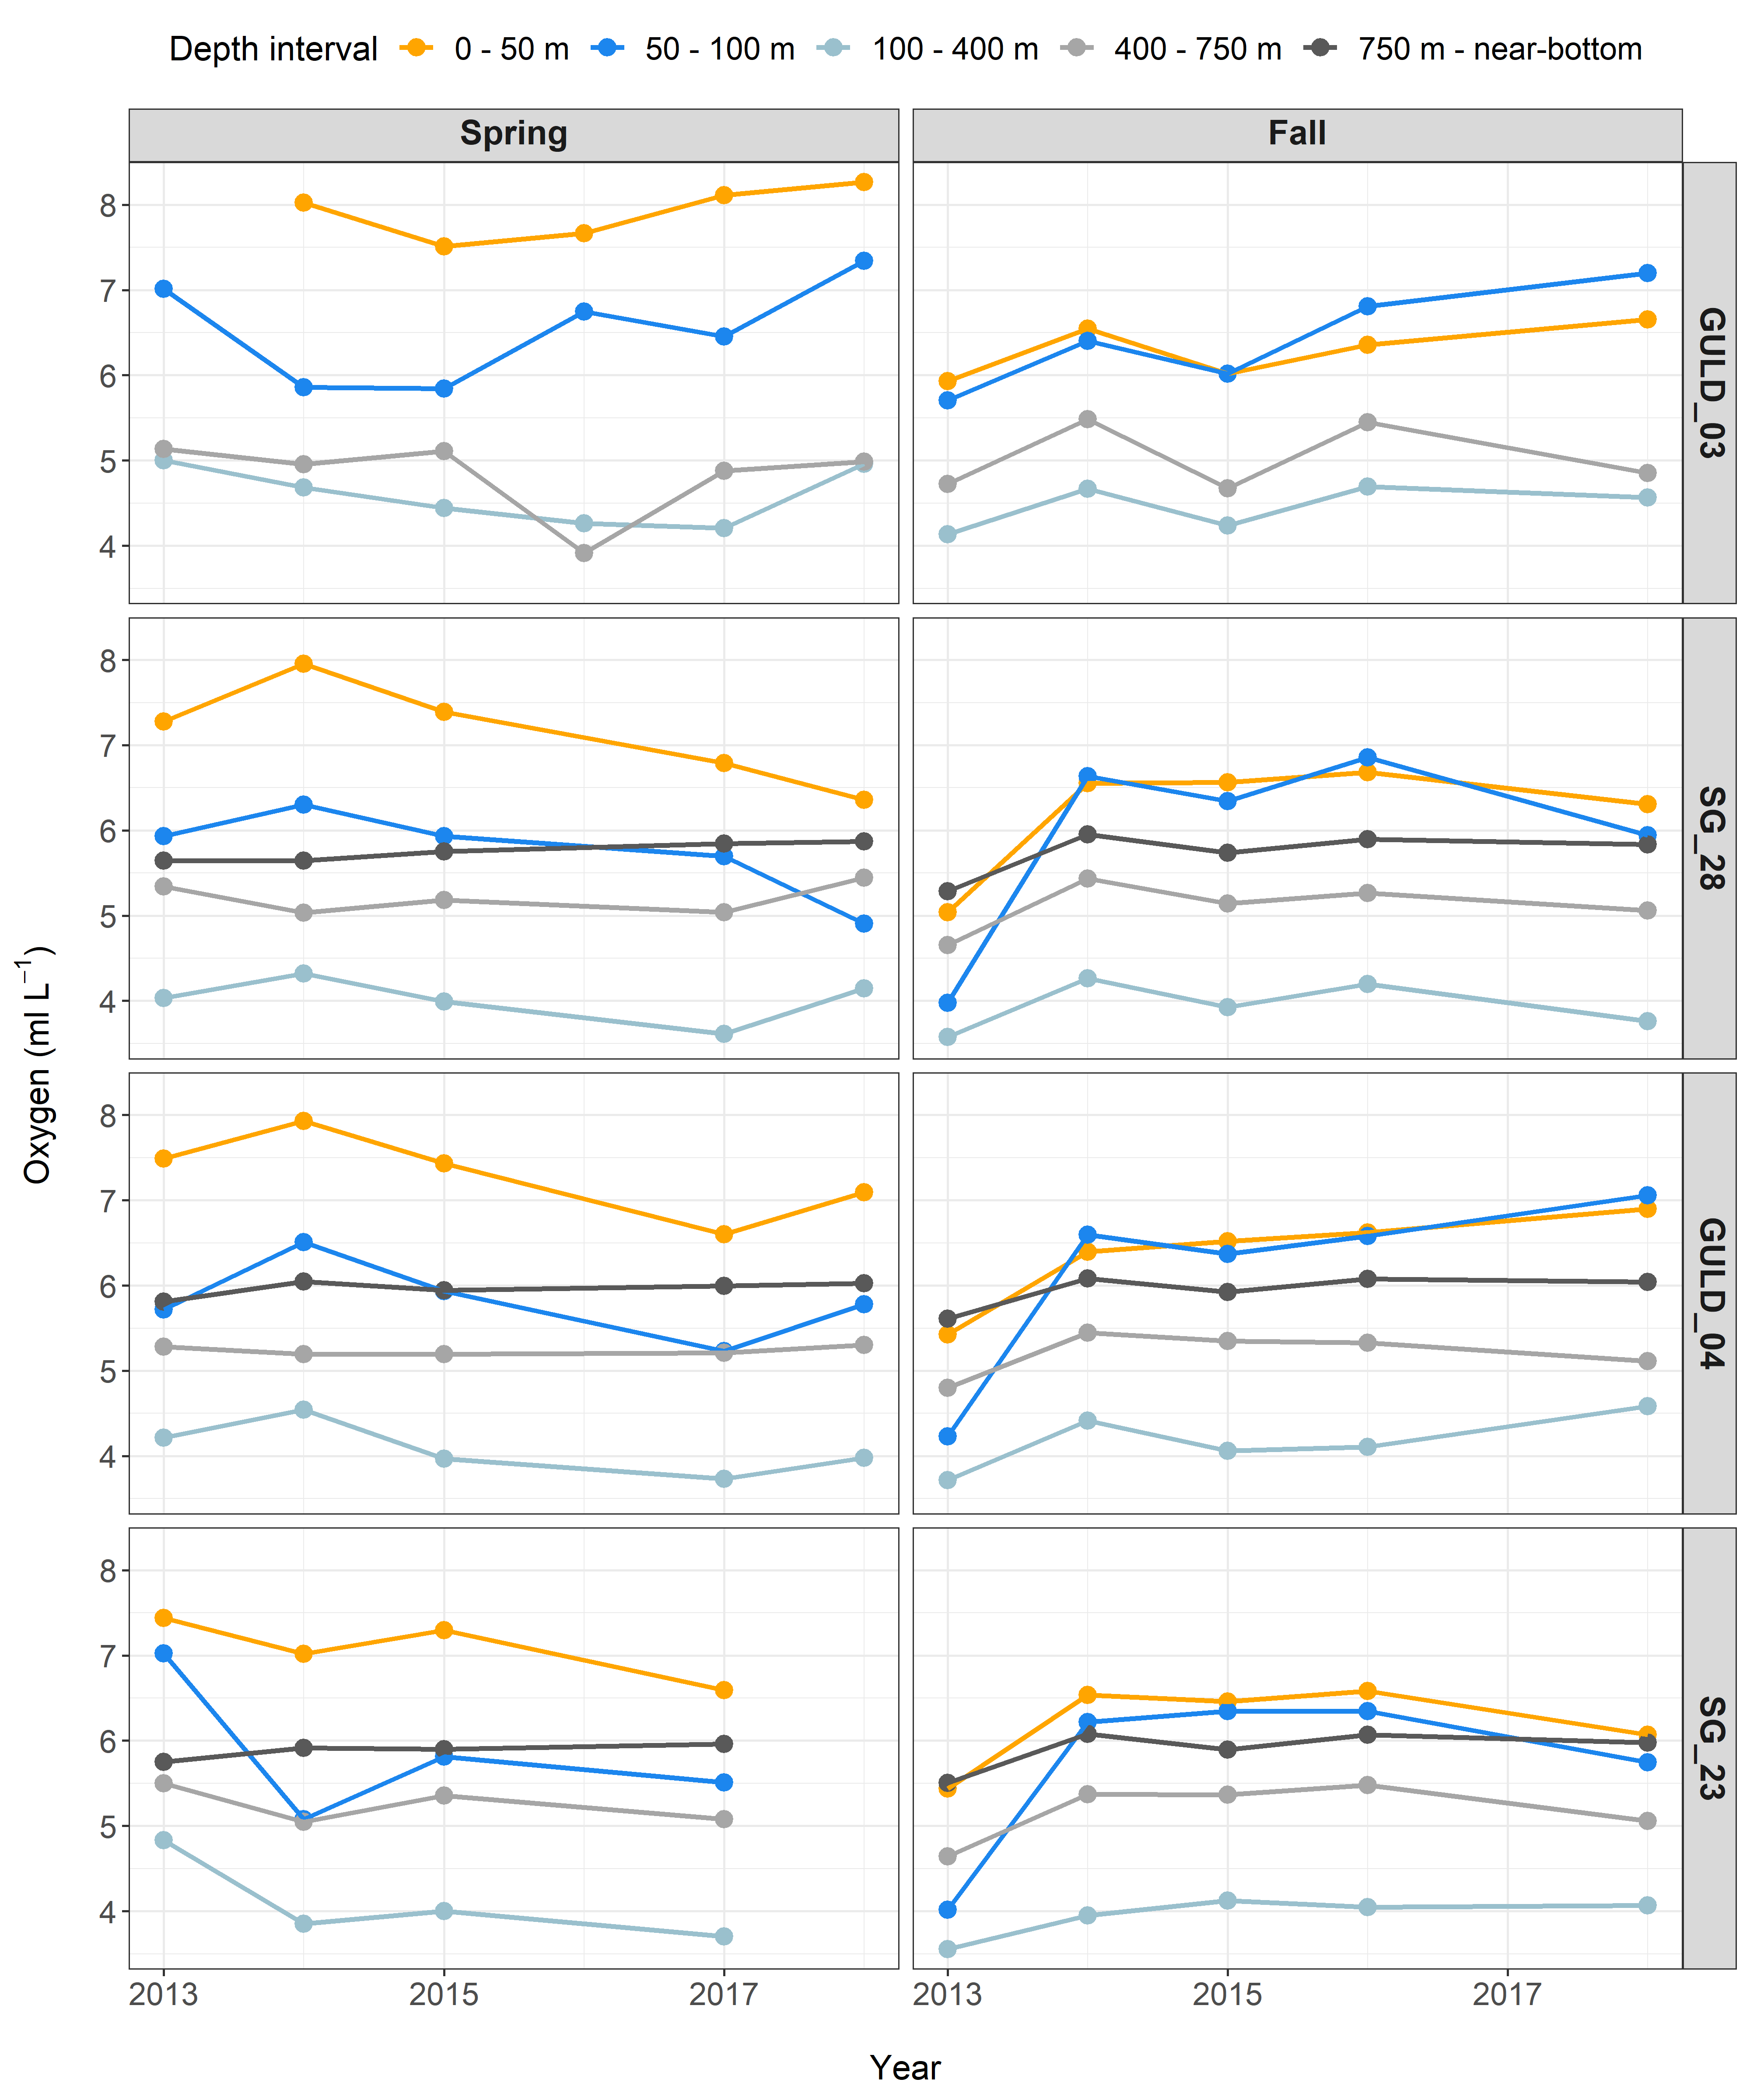
\includegraphics[width=6in]{figure/Figure12}}{Figure \ref{fig:figure12}} 

}

\caption{Changes in mean spring and fall dissolved oxygen concentration (ml L\textsuperscript{-1}) in five vertical depth intervals sampled at each of the four AZMP fixed stations in the Gully from 2013 to 2018. Only calibrated data from 2013 onward are included. Circles represent mean oxygen at each depth interval and year. Absent circles indicate that sampling did not occur at that station in that year. Note that the 400 to 750 m depth interval for GULD\_03 spans from \textgreater400 to near-bottom (up to 586 m). Oxygen data were not available for the surface layer (0 to 50 m) at GULD\_03 in 2013.}\label{fig:figure12}
\end{figure}
\clearpage


\begin{landscapepage}
\begin{figure}[htb]

{\centering \pdftooltip{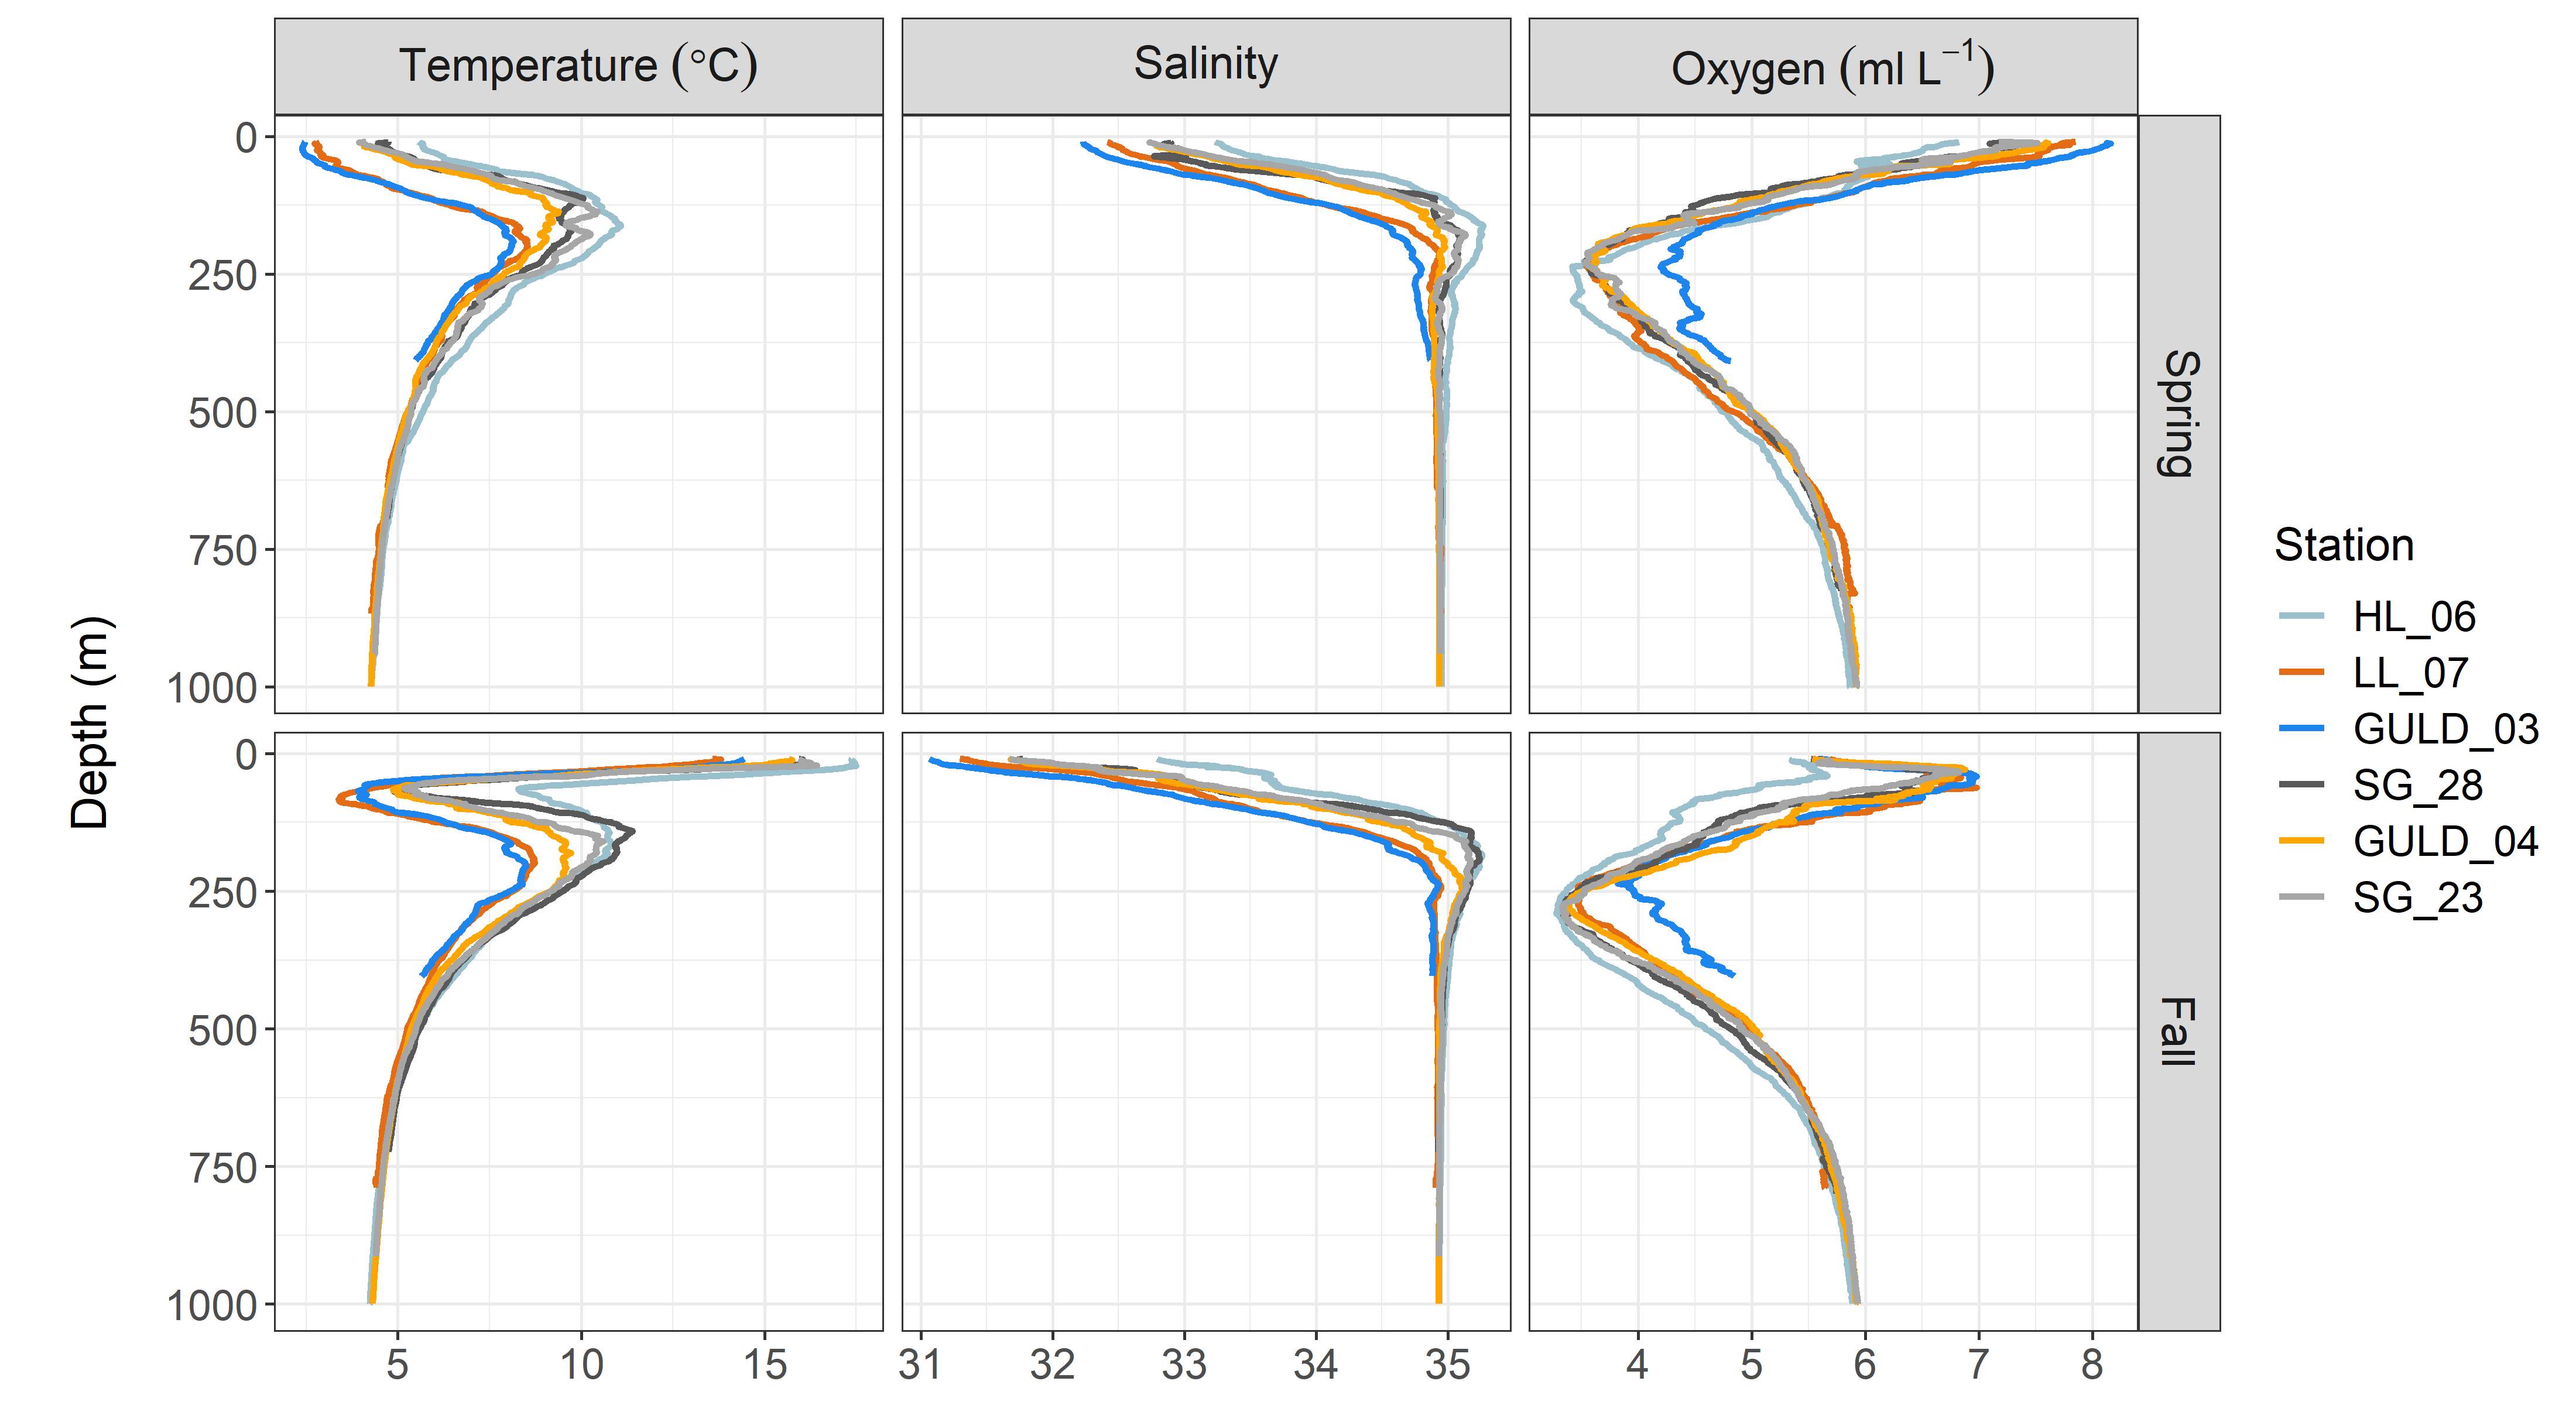
\includegraphics[width=9.5in]{figure/Figure13}}{Figure \ref{fig:figure13}} 

}

\caption{Comparison average temperature (\(\degree\)C), salinity, and dissolved oxygen (ml L\textsuperscript{-1}) to 1000 m on the four AZMP fixed stations in the Gully, and stations upstream (LL\_07) and downstream (HL\_06) of the Gully. Data were collected in the spring (April) and fall (September and October) between 2000 to 2018 for GULD\_03, GULD\_04, HL\_06, and LL\_07, and 2007 to 2018 for SG\_23 and SG\_28 (with slight variations between seasons). Oxygen data presented for each station is from 2013 onward.}\label{fig:figure13}
\end{figure}
\end{landscapepage}
\clearpage


\begin{figure}[htb]

{\centering \pdftooltip{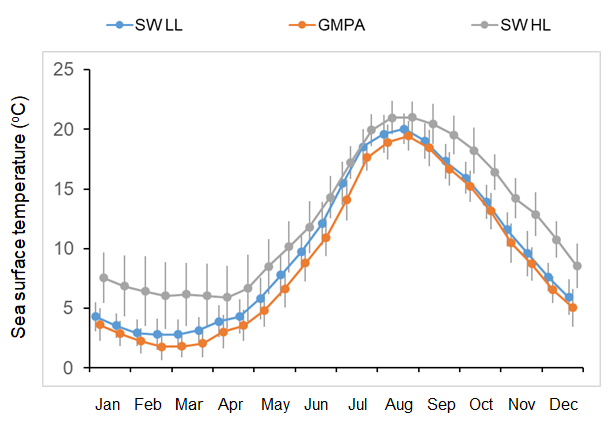
\includegraphics[width=6in]{figure/Figure14}}{Figure \ref{fig:figure14}} 

}

\caption{Remotely-sensed bi-monthly average sea surface temperatures (1998 to 2018, mean \(\pm\) S.D.) in the slope water satellite areas off the eastern (SW LL) and central (SW HL) Scotian Shelf and in the Gully MPA (GMPA).}\label{fig:figure14}
\end{figure}
\clearpage


\begin{figure}[htb]

{\centering \pdftooltip{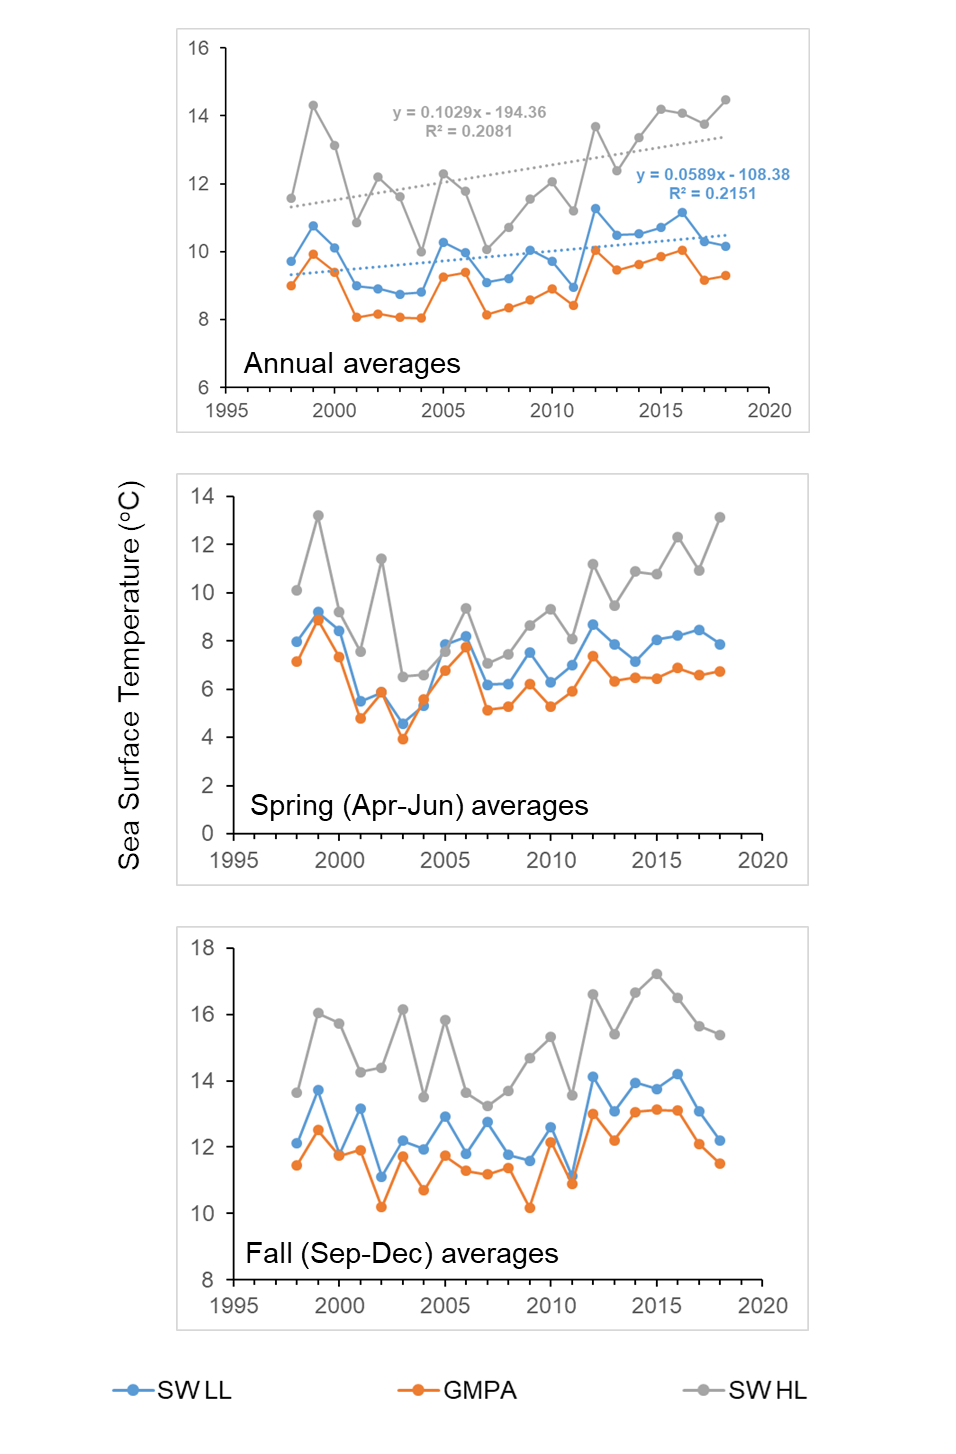
\includegraphics[width=5.0in]{figure/Figure15}}{Figure \ref{fig:figure15}} 

}

\caption{Time series for remotely-sensed annual, spring and fall average sea surface temperatures in slope water satellite areas off the eastern (SW LL) and central (SW HL) Scotian Shelf and in the Gully MPA (GMPA). Lines and equations are shown for significant trends.}\label{fig:figure15}
\end{figure}
\clearpage


\begin{figure}[htb]

{\centering \pdftooltip{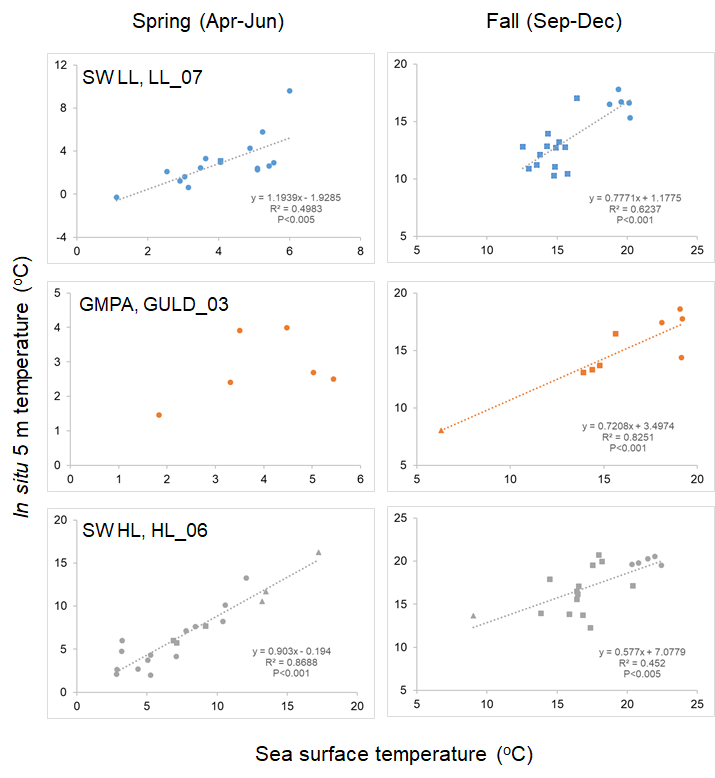
\includegraphics[width=6in]{figure/Figure16}}{Figure \ref{fig:figure16}} 

}

\caption{Relationships between \emph{in situ} 5 m temperatures measured at HL\_06, GULD\_03 and LL\_07 during AZMP and other sampling missions and remotely-sensed sea surface temperatures averaged for the corresponding months/years for the SW HL, GMPA and SW LL satellite areas. Filled circles, squares and triangles represent measurements in April, May and June, respectively, in spring, and in September, October and December, respectively, in fall.}\label{fig:figure16}
\end{figure}
\clearpage


\begin{landscapepage}
\begin{figure}[htb]

{\centering \pdftooltip{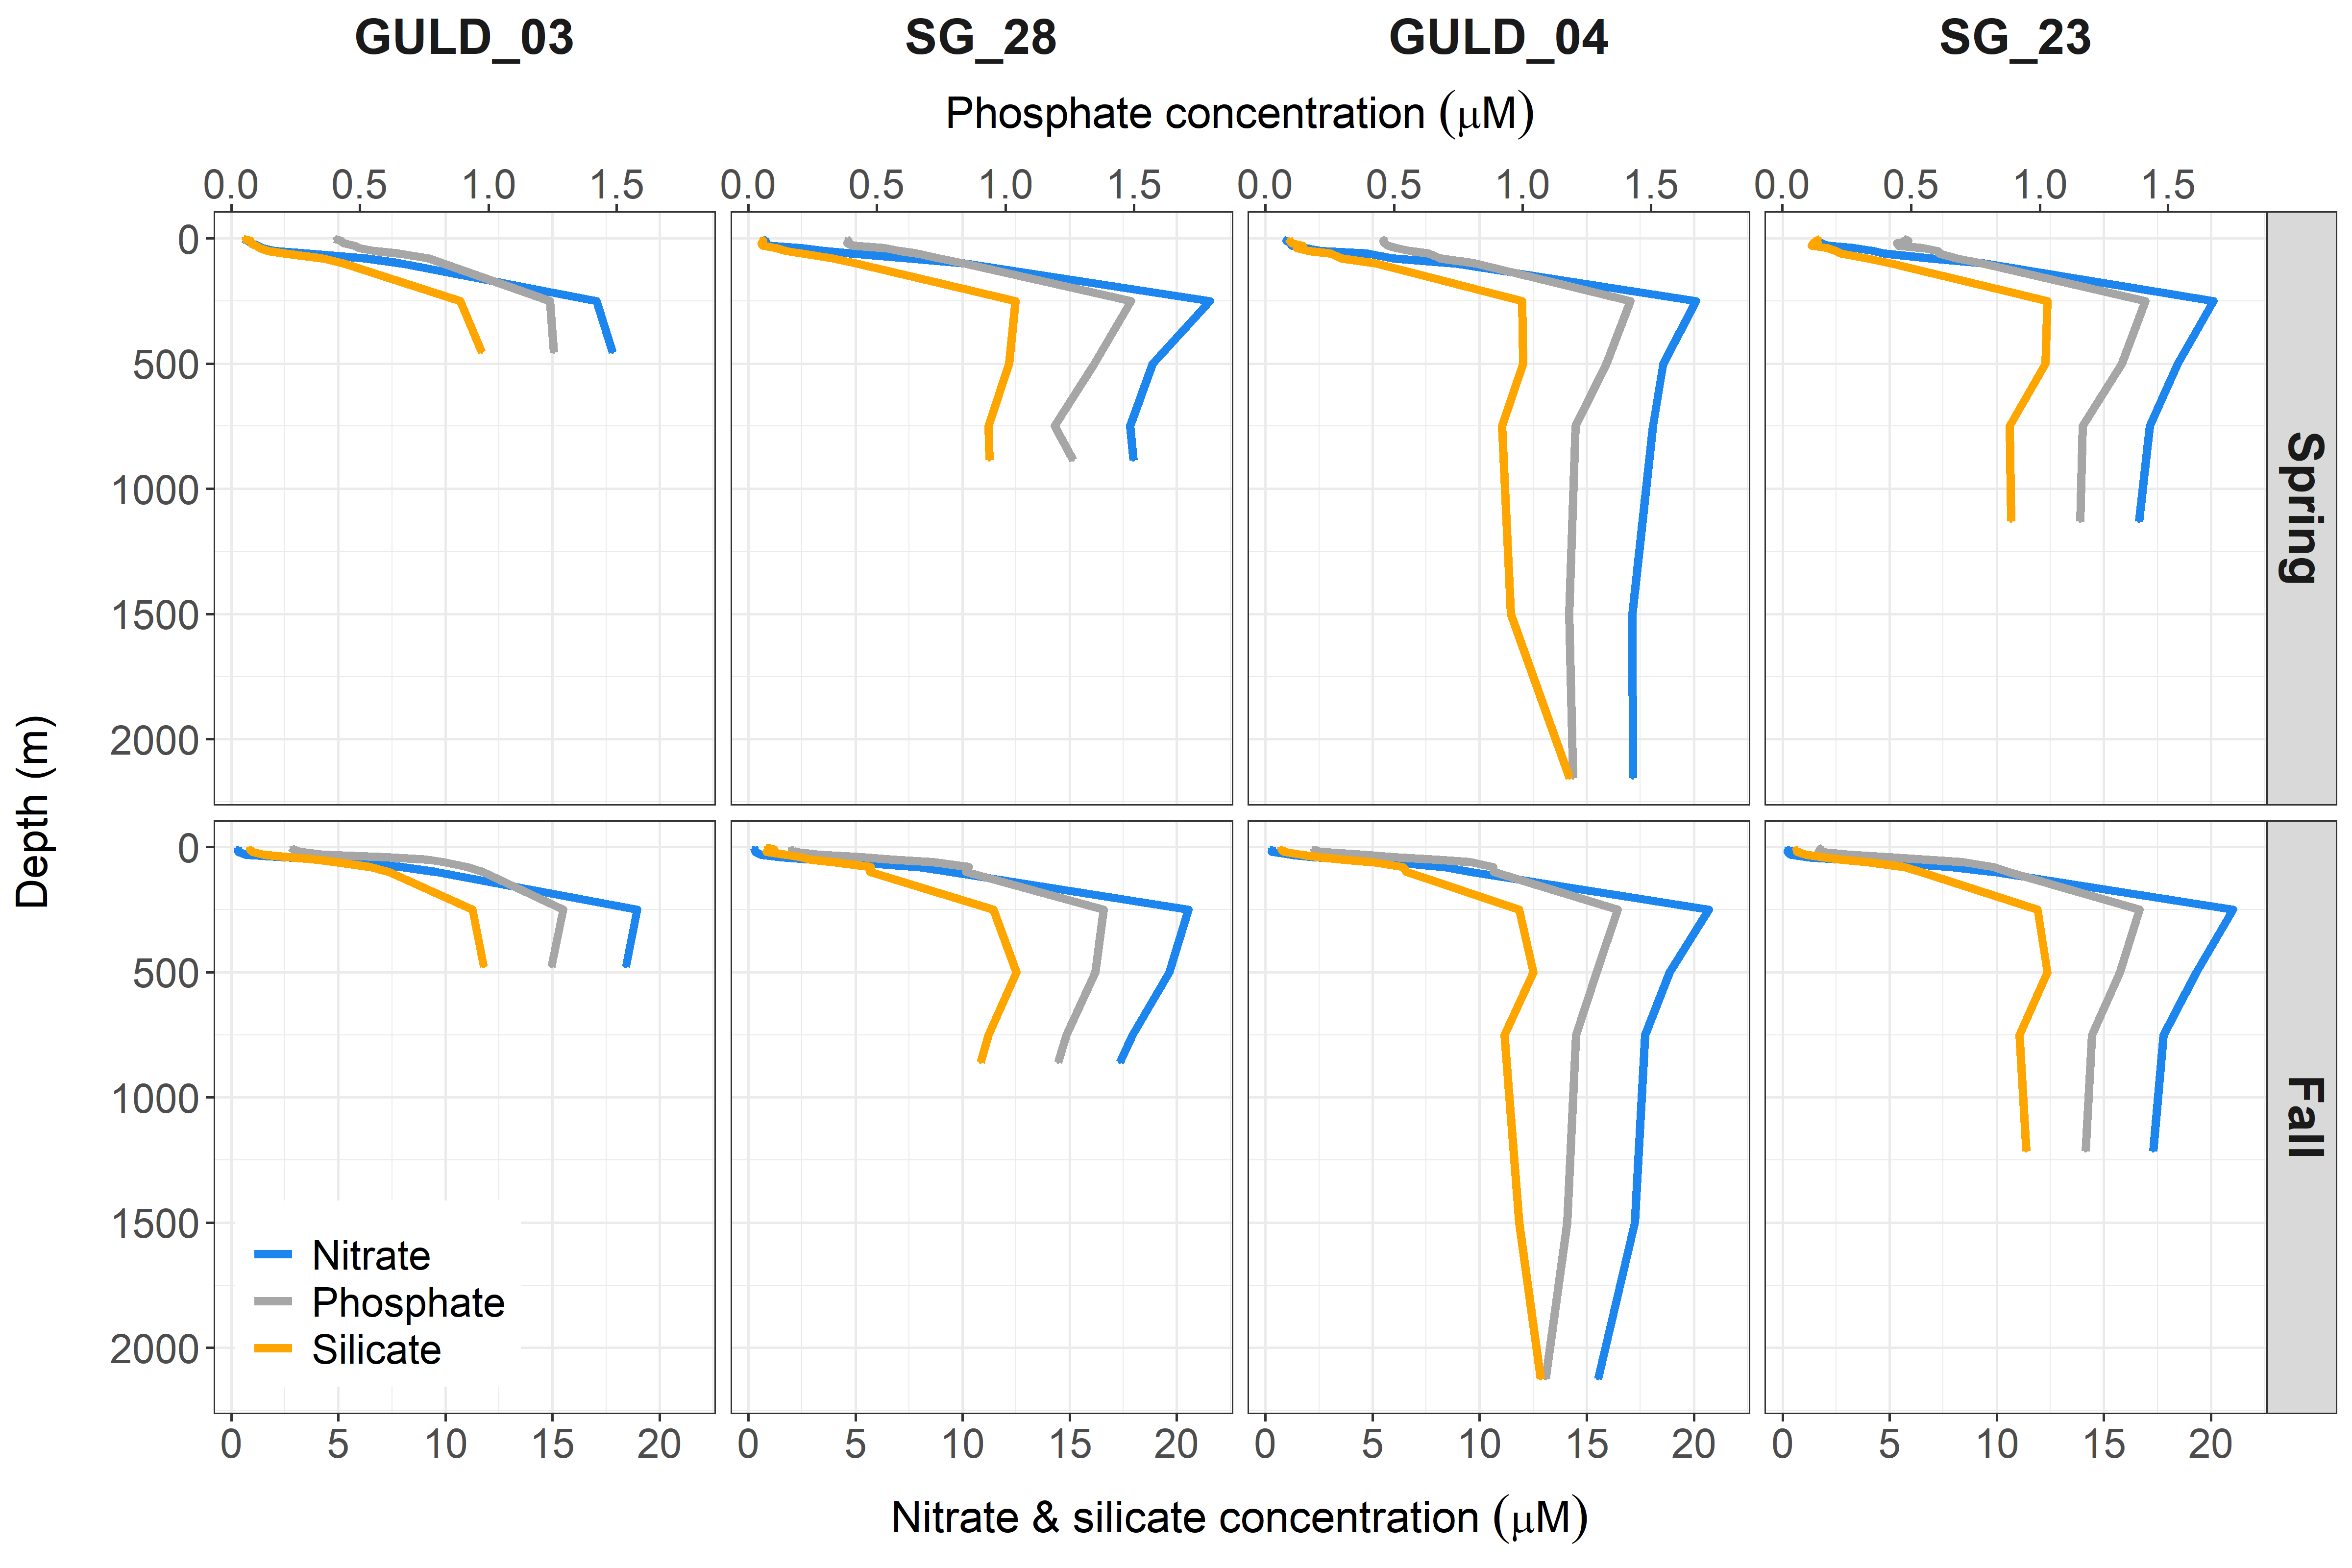
\includegraphics[width=7.5in]{figure/Figure17}}{Figure \ref{fig:figure17}} 

}

\caption{Mean vertical structure in spring and fall nitrate, phosphate, and silicate concentration (\(\mu\)M) at the four AZMP fixed stations in the Gully. Mean values were calculated at each standard nominal depth (see Table~\ref{tab:table3}) and connected with trend lines. Near-bottom sample depth varied between years and seasons and was represented by the average depth of the near-bottom bottle collected across all years (see subsection~\ref{sec:chemical-data} of the Data and Methodology section).}\label{fig:figure17}
\end{figure}
\end{landscapepage}
\clearpage


\begin{figure}[htb]

{\centering \pdftooltip{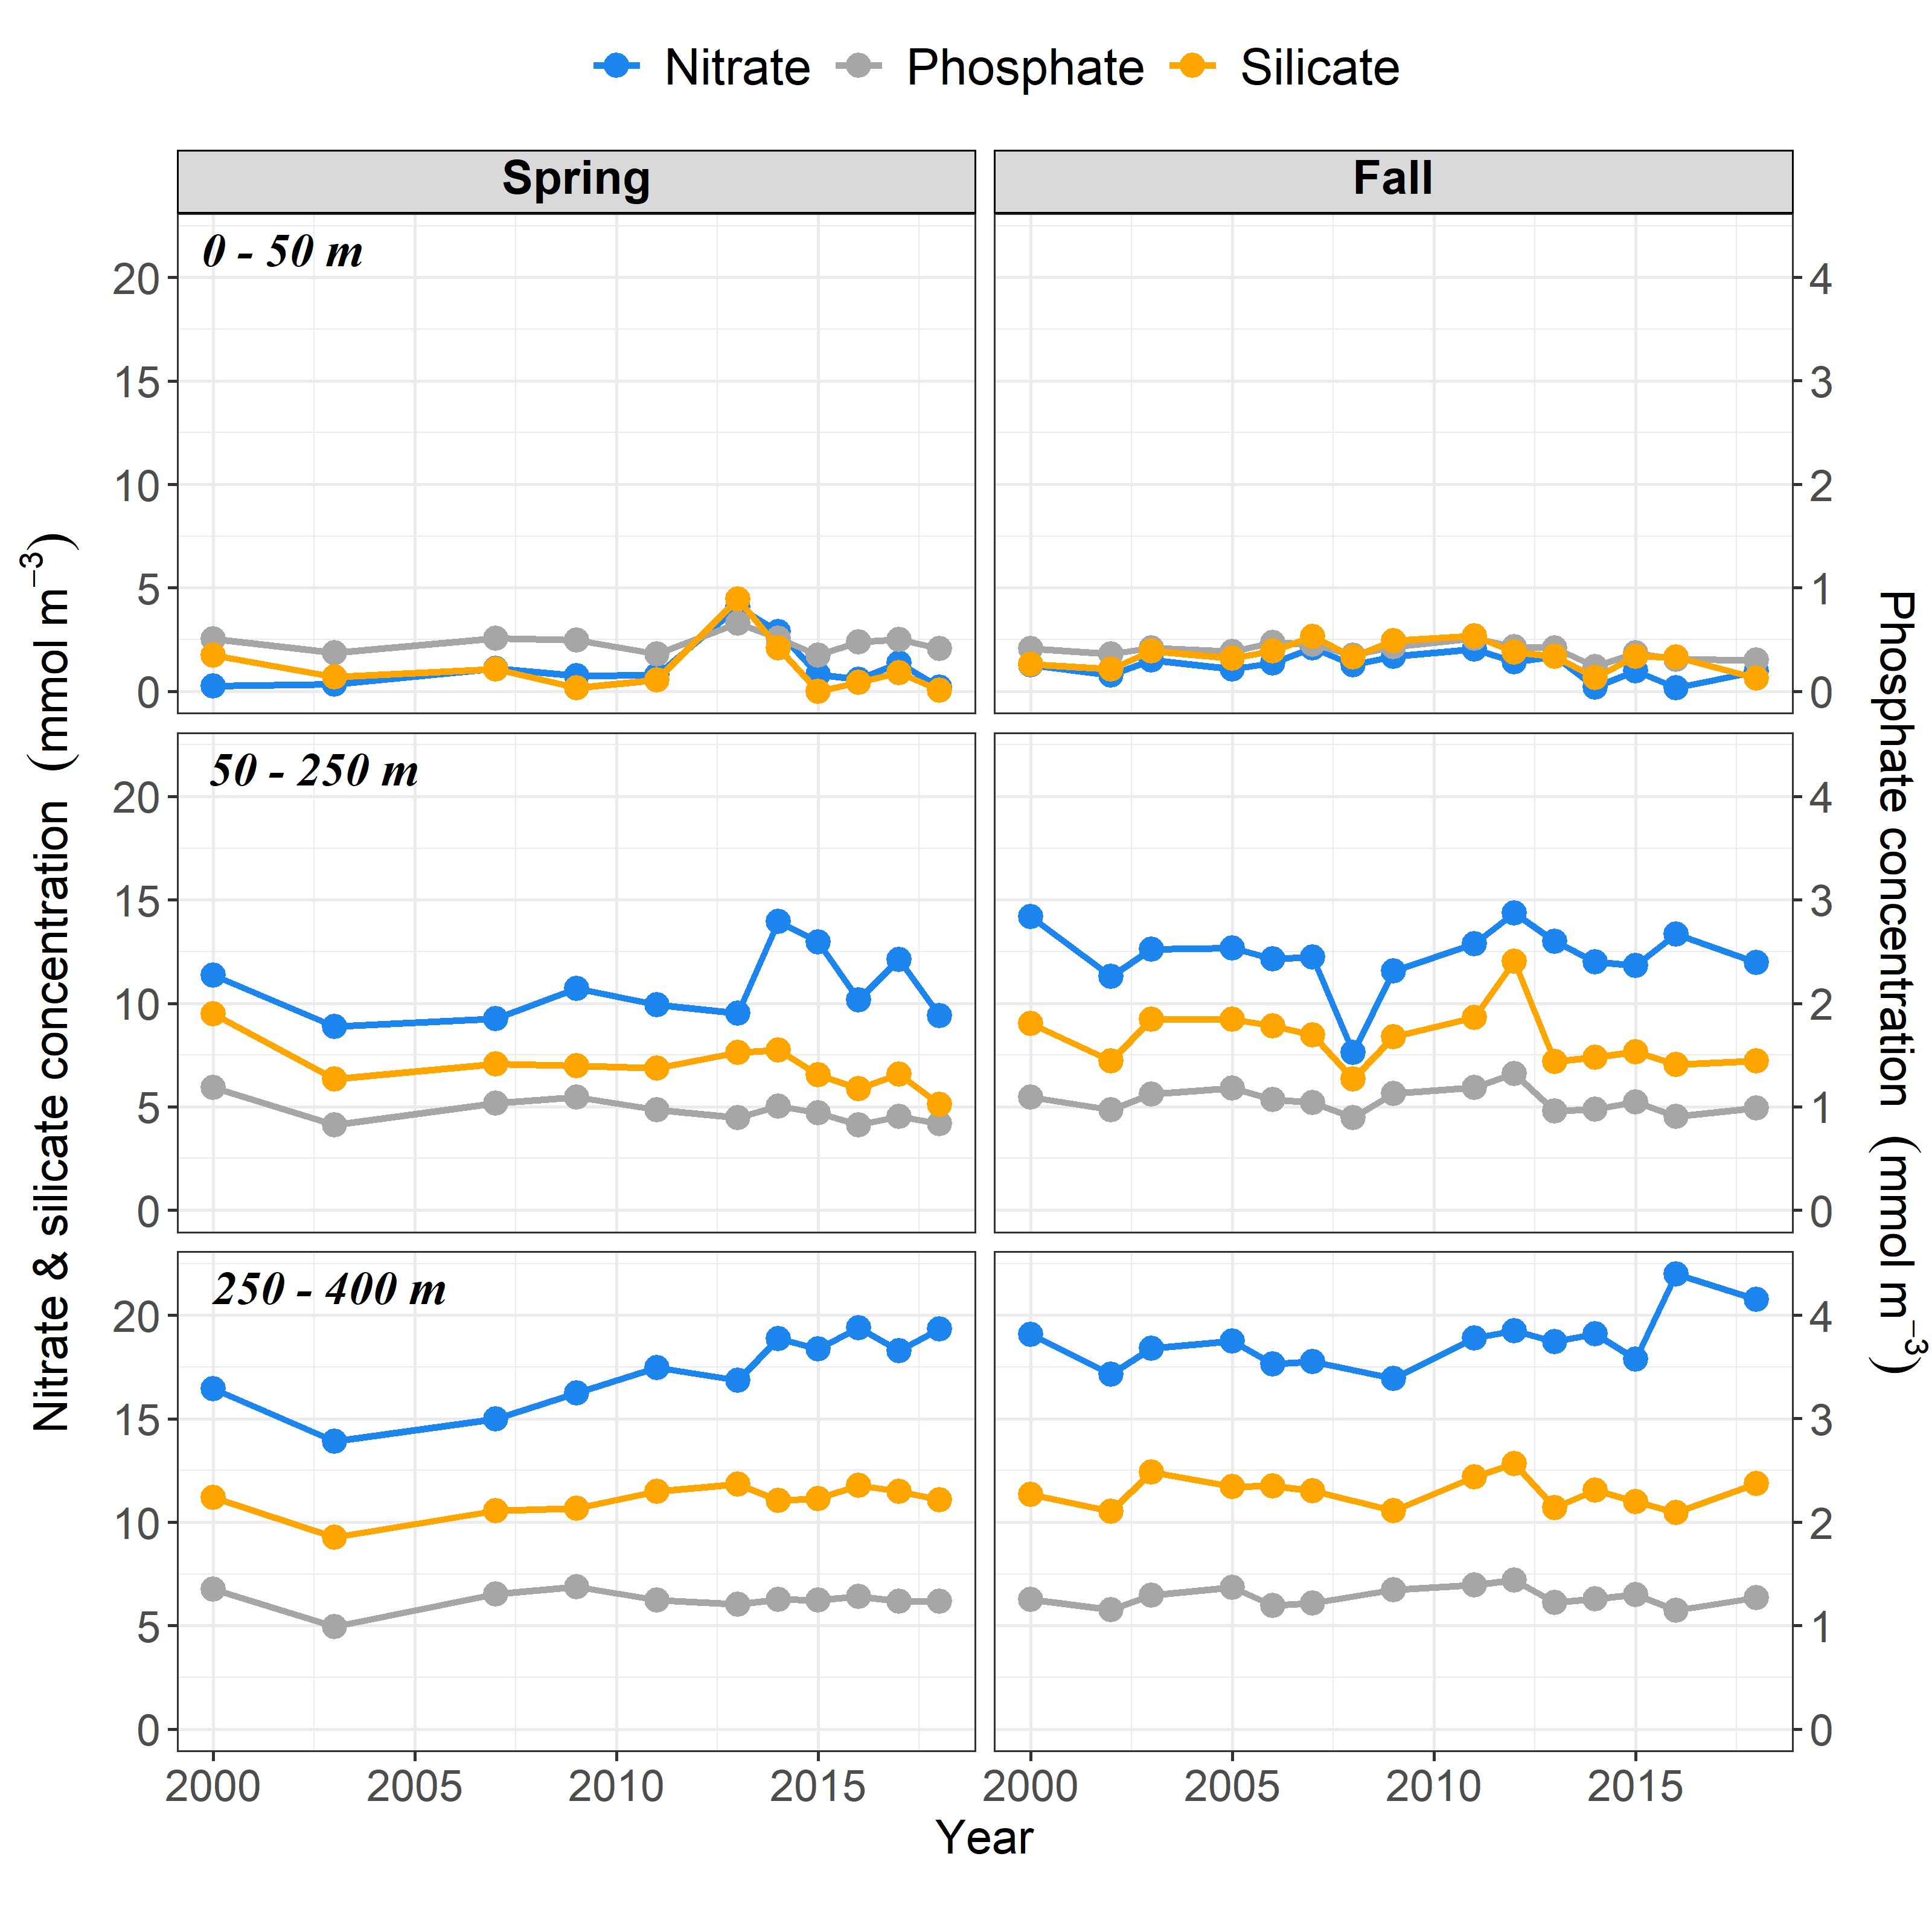
\includegraphics[width=6in]{figure/Figure18}}{Figure \ref{fig:figure18}} 

}

\caption{Vertically-integrated nitrate, phosphate, and silicate concentration (mmol m\textsuperscript{-3}) sampled in the spring (April) and fall (September and October) at AZMP fixed station GULD\_03. Circles represent the vertically-integrated nutrient inventories for each depth interval and year. Absent circles indicate that sampling did not occur within that particular depth interval and/or year.}\label{fig:figure18}
\end{figure}
\clearpage


\begin{figure}[htb]

{\centering \pdftooltip{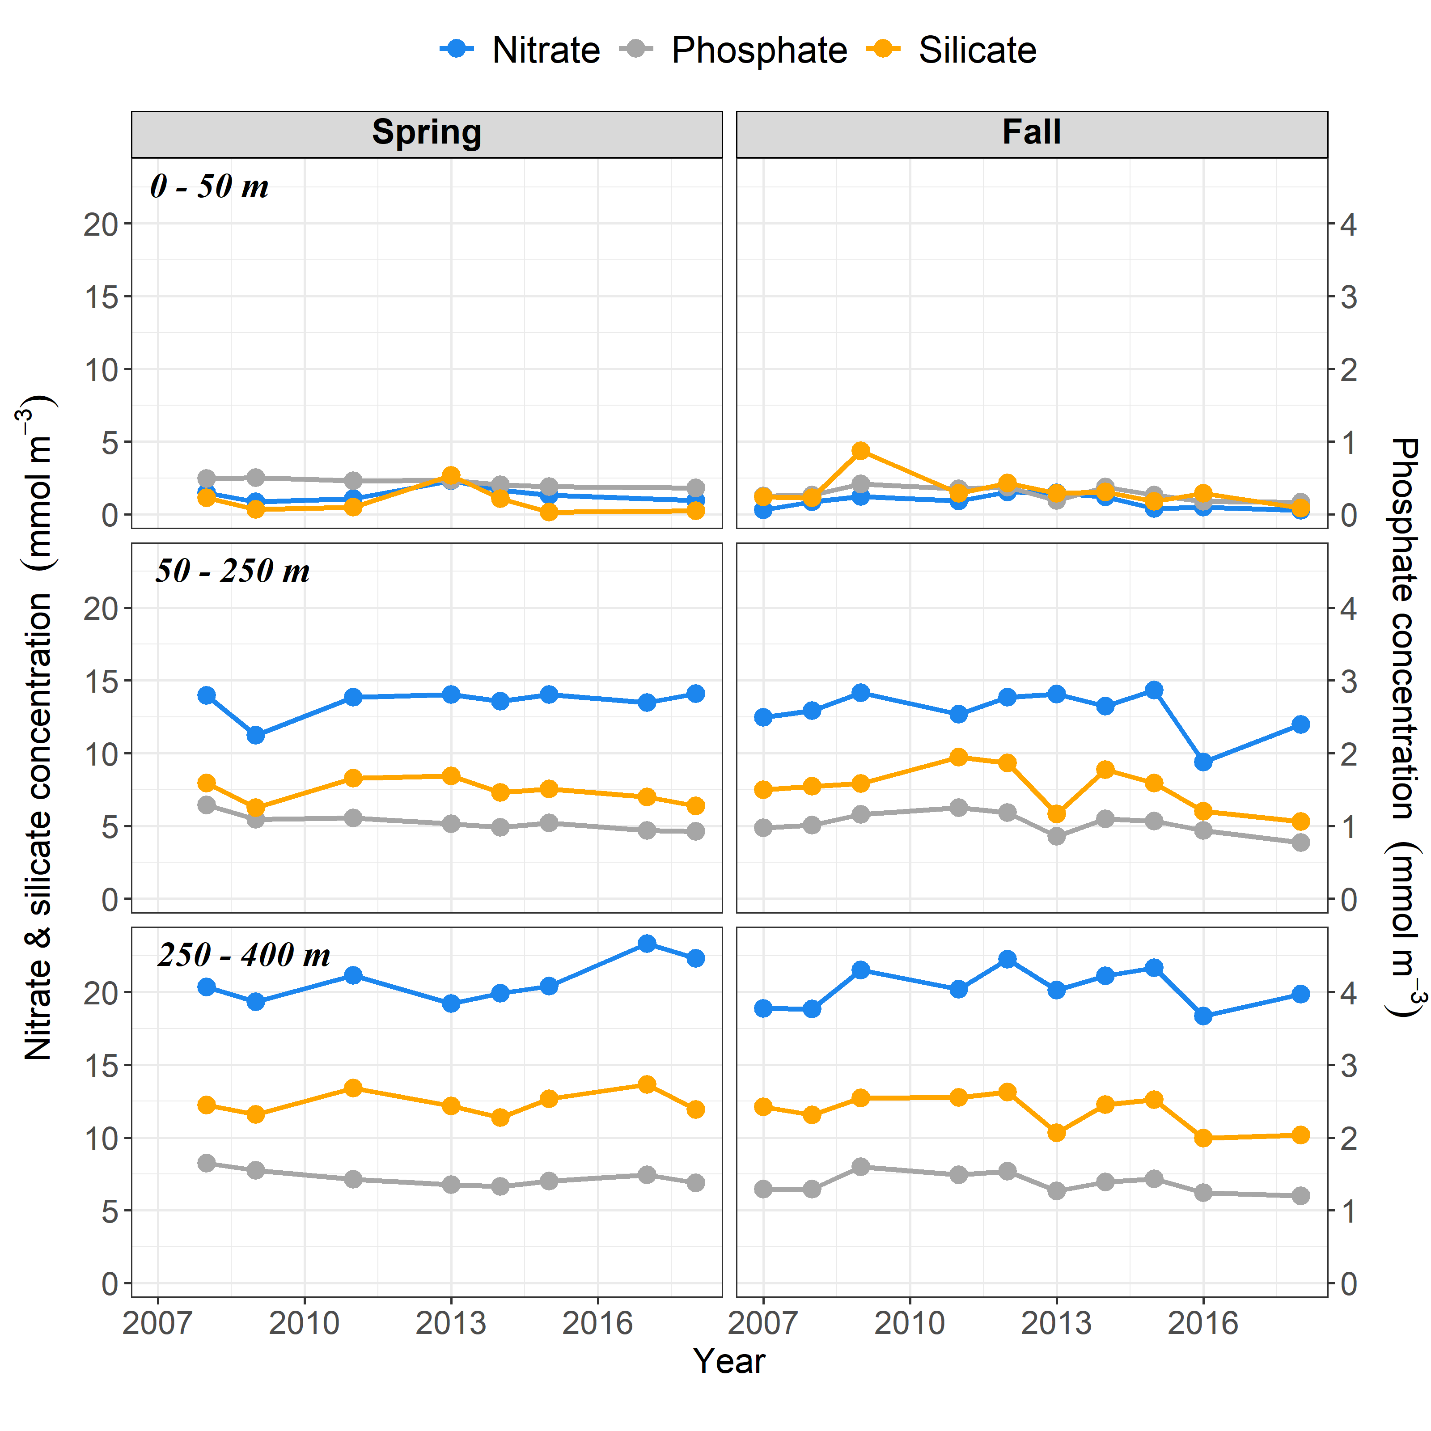
\includegraphics[width=6in]{figure/Figure19}}{Figure \ref{fig:figure19}} 

}

\caption{Vertically-integrated nitrate, phosphate, and silicate concentration (mmol m\textsuperscript{-3}) sampled in the spring (April) and fall (September and October) at AZMP fixed station SG\_28. Circles represent the vertically-integrated nutrient inventories for each depth interval and year. Absent circles indicate that sampling did not occur within that particular depth interval and/or year.}\label{fig:figure19}
\end{figure}
\clearpage


\begin{figure}[htb]

{\centering \pdftooltip{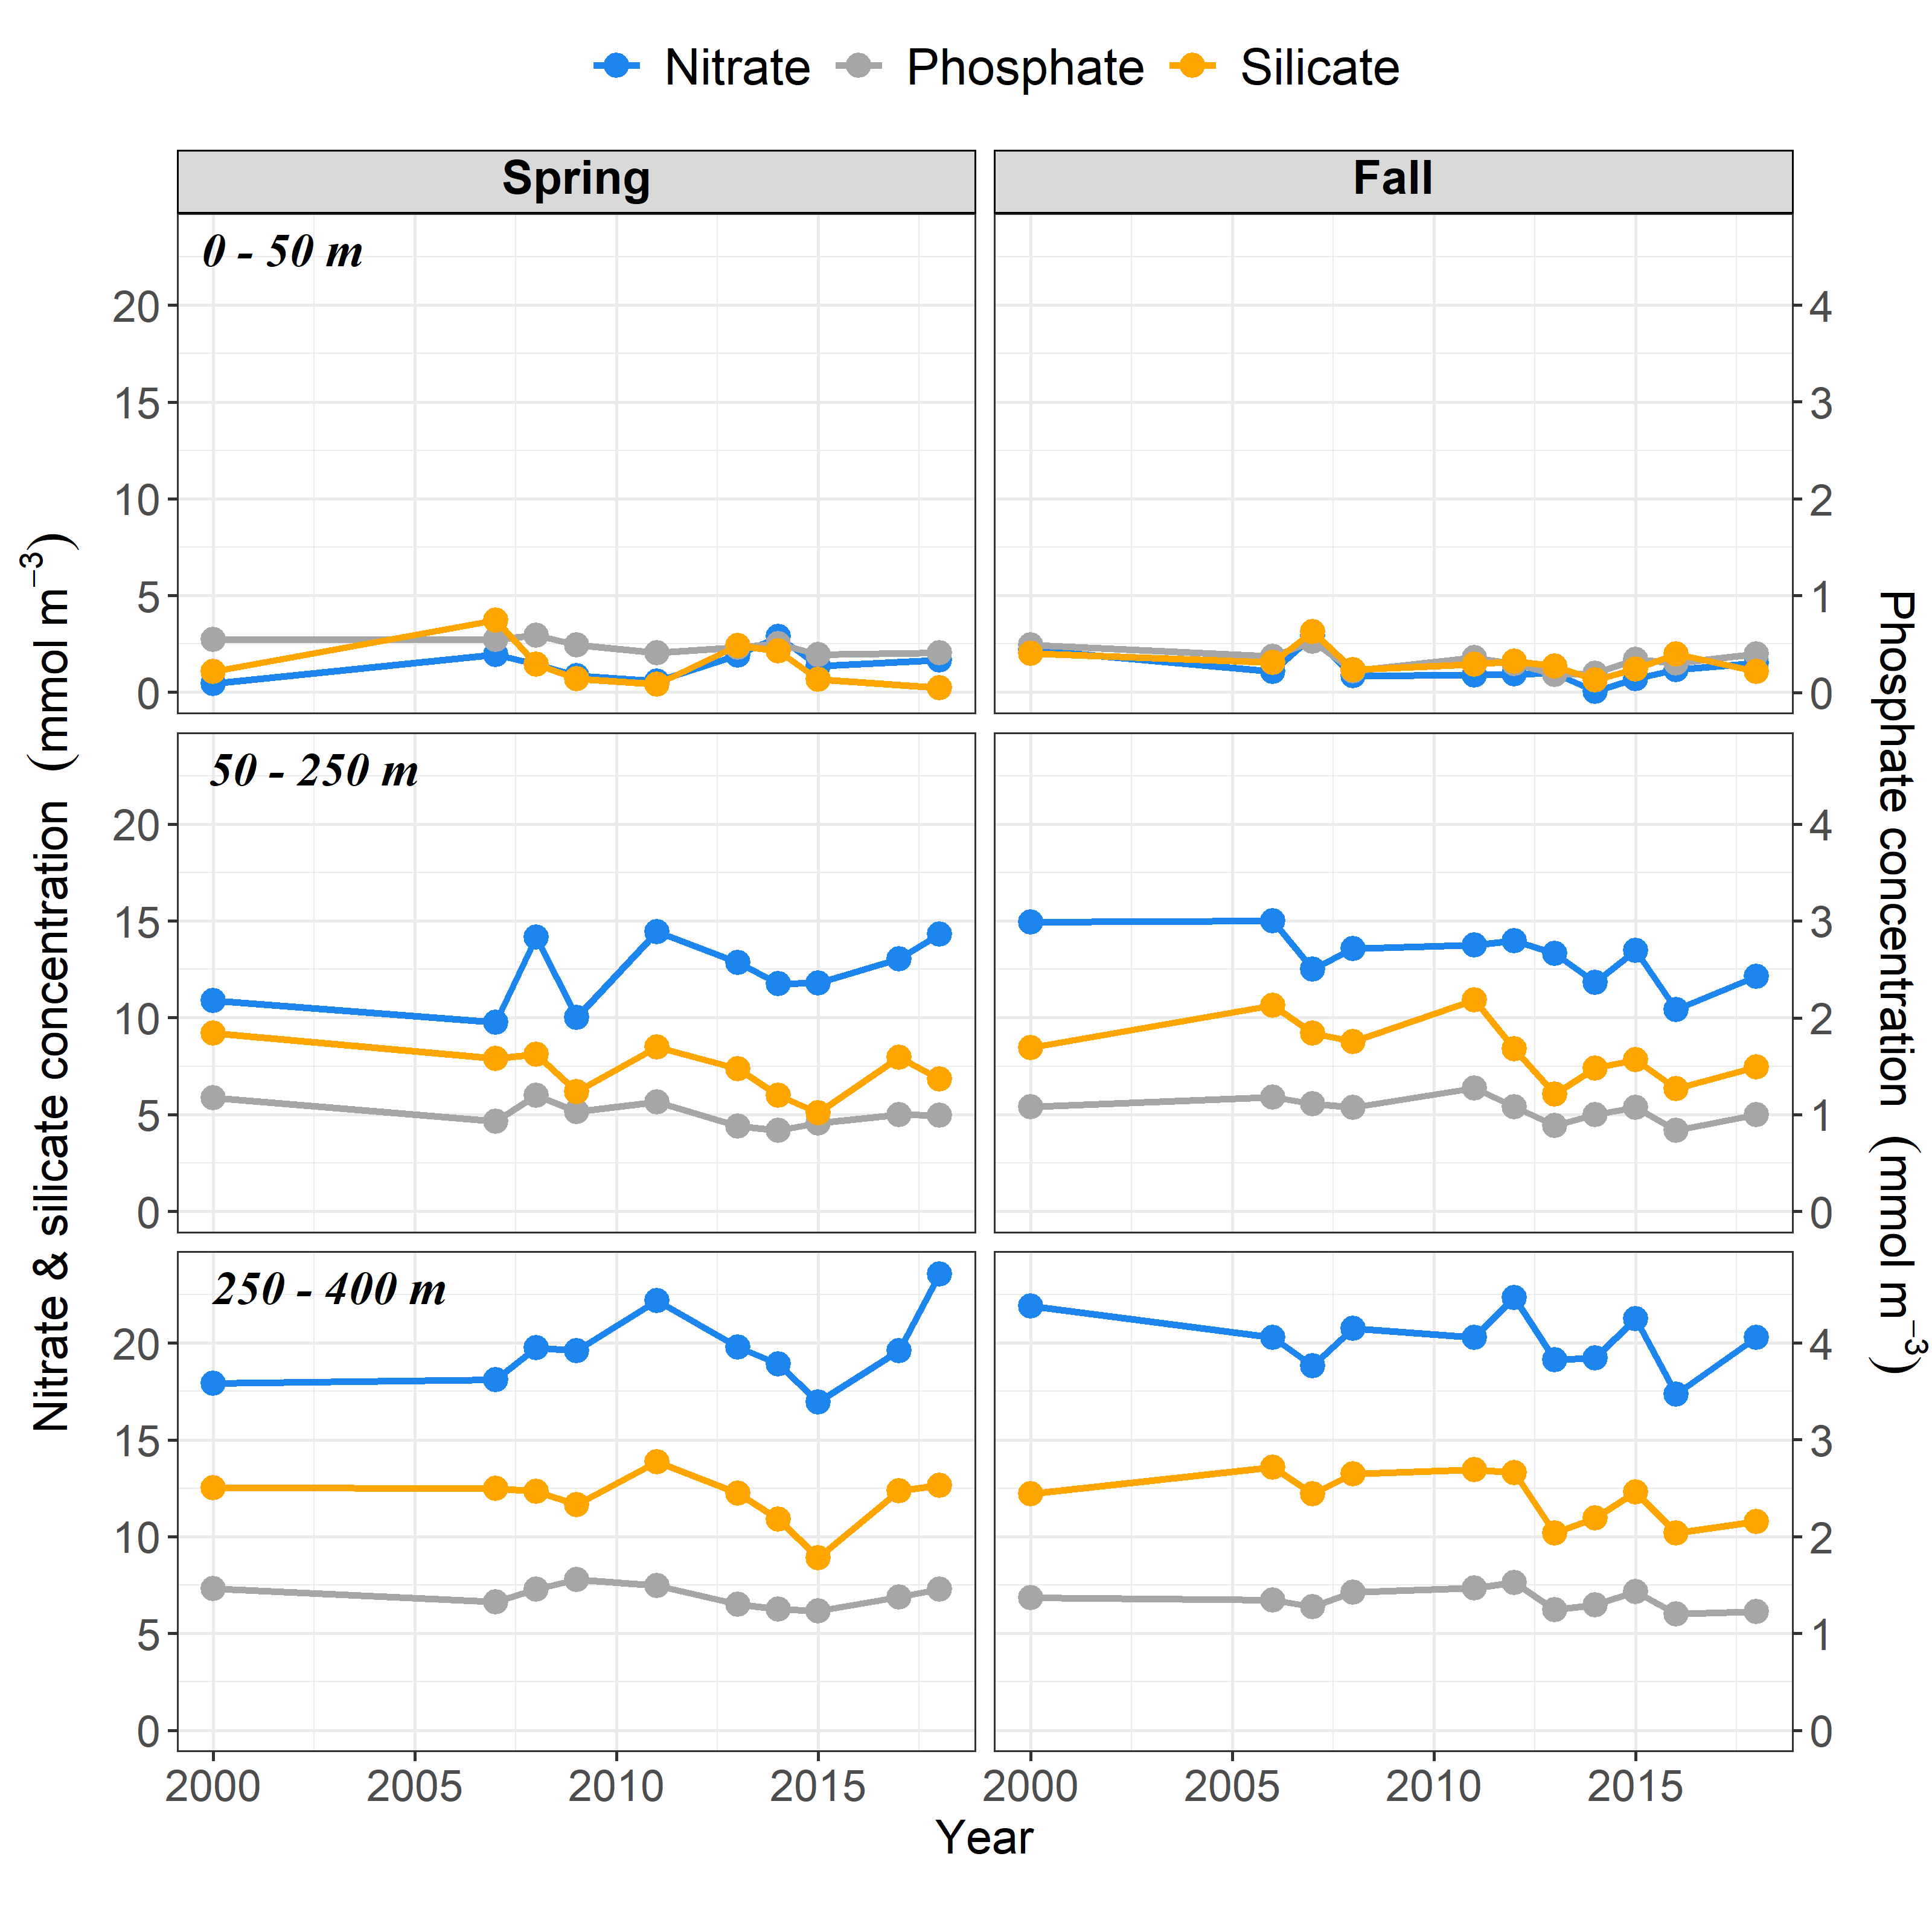
\includegraphics[width=6in]{figure/Figure20}}{Figure \ref{fig:figure20}} 

}

\caption{Vertically-integrated nitrate, phosphate, and silicate concentration (mmol m\textsuperscript{-3}) sampled in the spring (April) and fall (September and October) at AZMP fixed station GULD\_04. Circles represent the vertically-integrated nutrient inventories for each depth interval and year. Absent circles indicate that sampling did not occur within that particular depth interval and/or year.}\label{fig:figure20}
\end{figure}
\clearpage


\begin{figure}[htb]

{\centering \pdftooltip{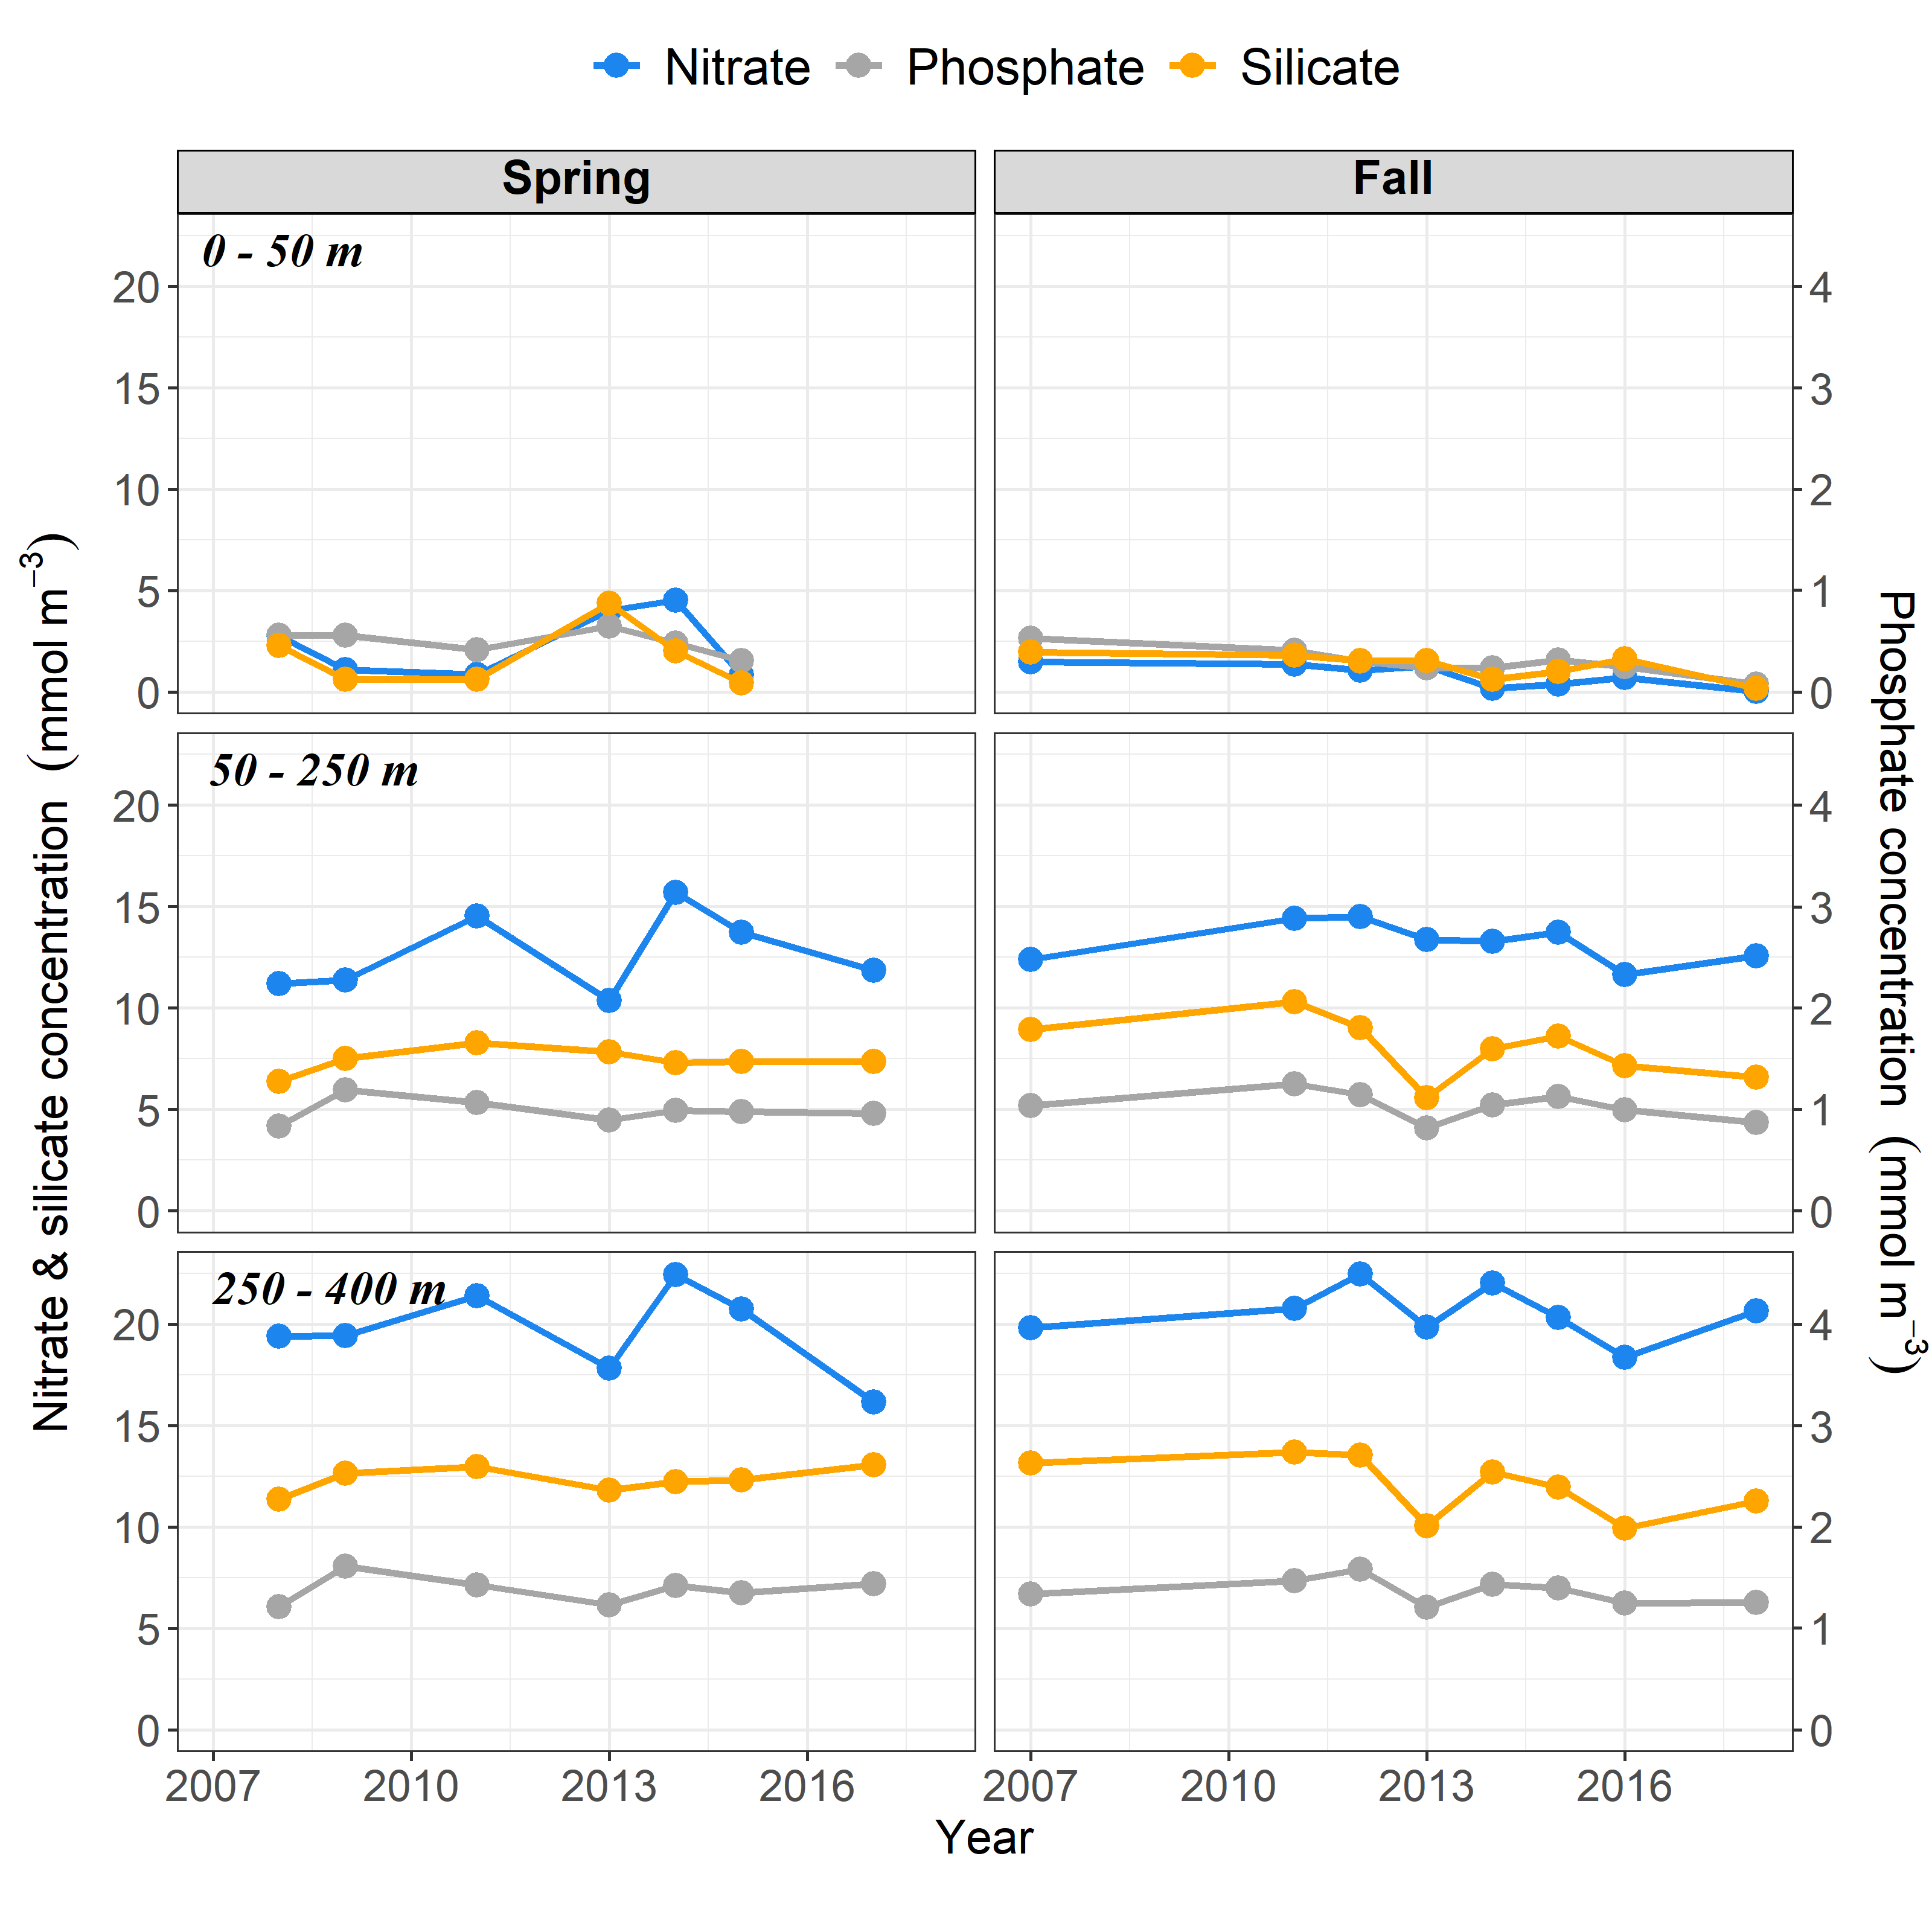
\includegraphics[width=6in]{figure/Figure21}}{Figure \ref{fig:figure21}} 

}

\caption{Vertically-integrated nitrate, phosphate, and silicate concentration (mmol m\textsuperscript{-3}) sampled in the spring (April) and fall (September and October) at AZMP fixed station SG\_23. Circles represent the vertically-integrated nutrient inventories for each depth interval and year. Absent circles indicate that sampling did not occur within that particular depth interval and/or year.}\label{fig:figure21}
\end{figure}
\clearpage


\begin{landscapepage}
\begin{figure}[htb]

{\centering \pdftooltip{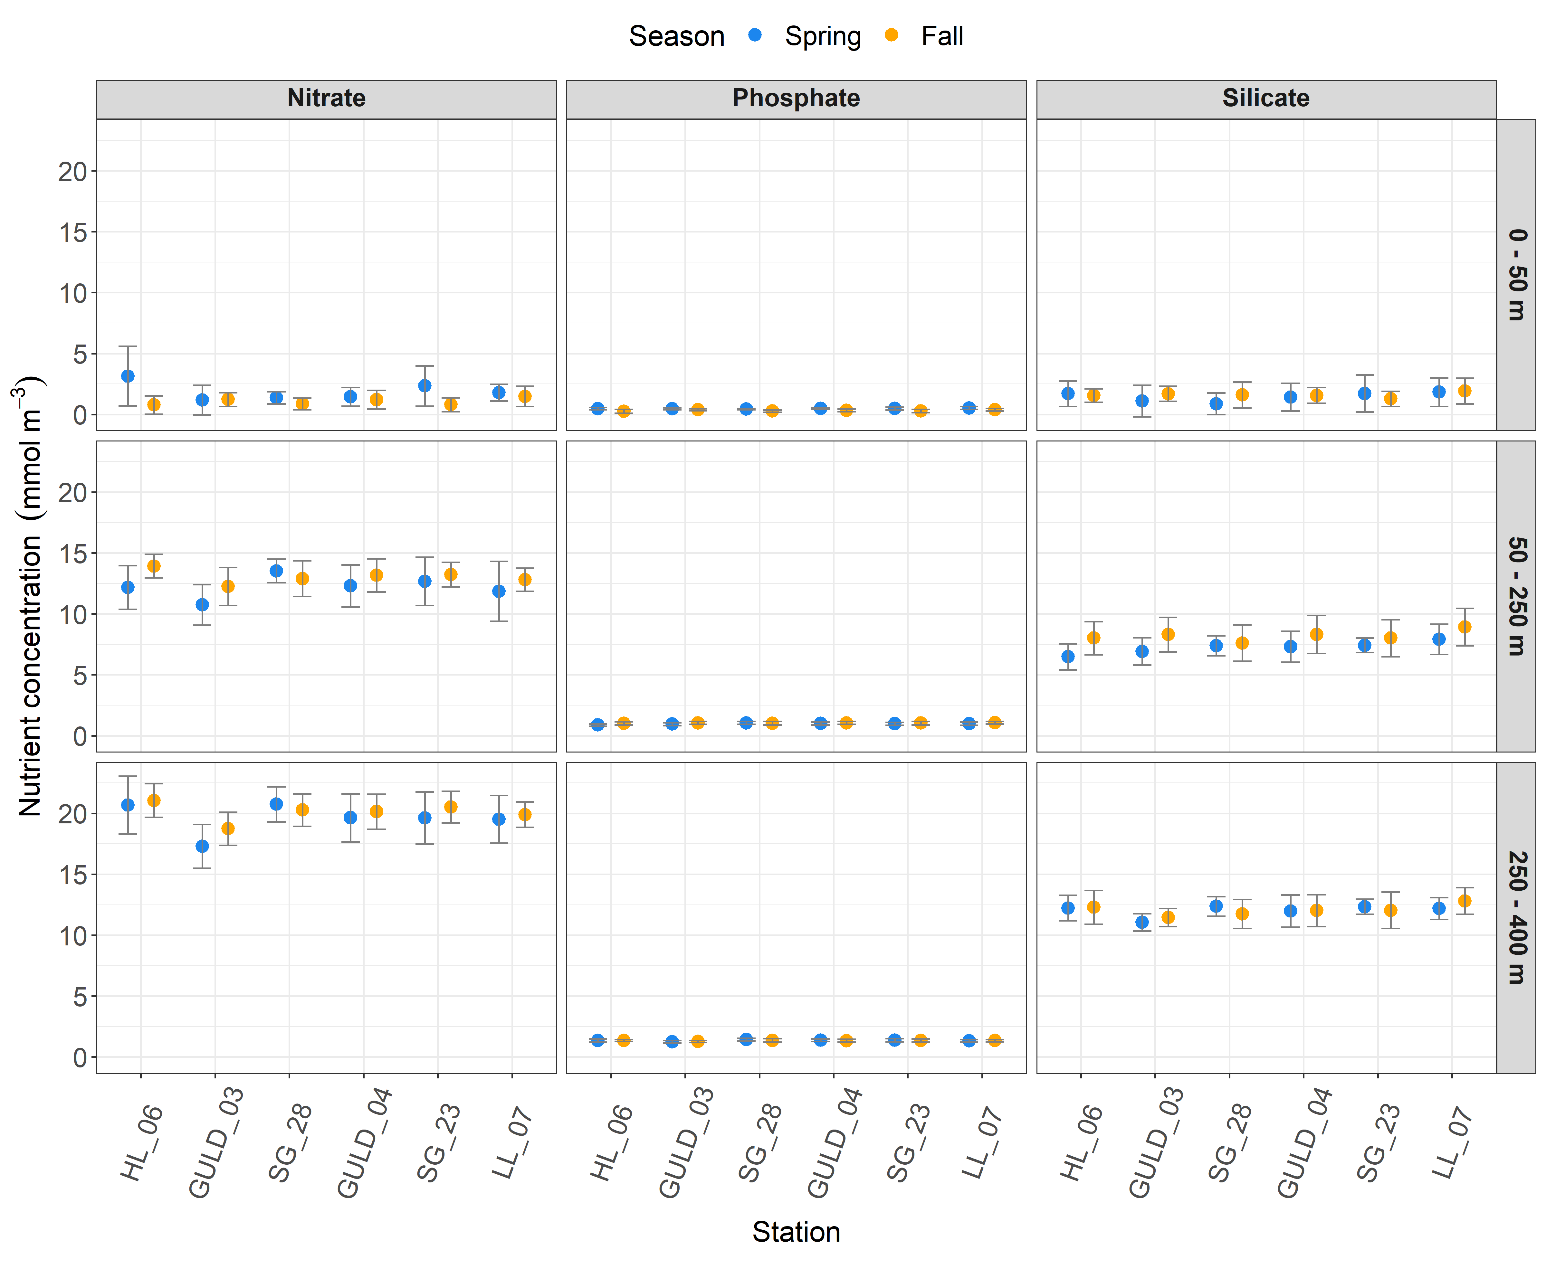
\includegraphics[width=6.5in]{figure/Figure22}}{Figure \ref{fig:figure22}} 

}

\caption{Mean nitrate, phosphate, and silicate concentration (mmol m\textsuperscript{-3}) in spring (blue circles) and fall (orange circles) at each of the four AZMP fixed stations in the Gully MPA, and stations upstream (LL\_07) and downstream (HL\_06) of the Gully. Error bars are \(\pm\) standard deviation. Data were collected in the spring (April) and fall (September and October) between 2000 to 2018 for GULD\_03, GULD\_04, HL\_06, and LL\_07, and 2007 to 2018 for SG\_23 and SG\_28 (with slight variations between seasons).}\label{fig:figure22}
\end{figure}
\end{landscapepage}
\clearpage


\begin{landscapepage}
\begin{figure}[htb]

{\centering \pdftooltip{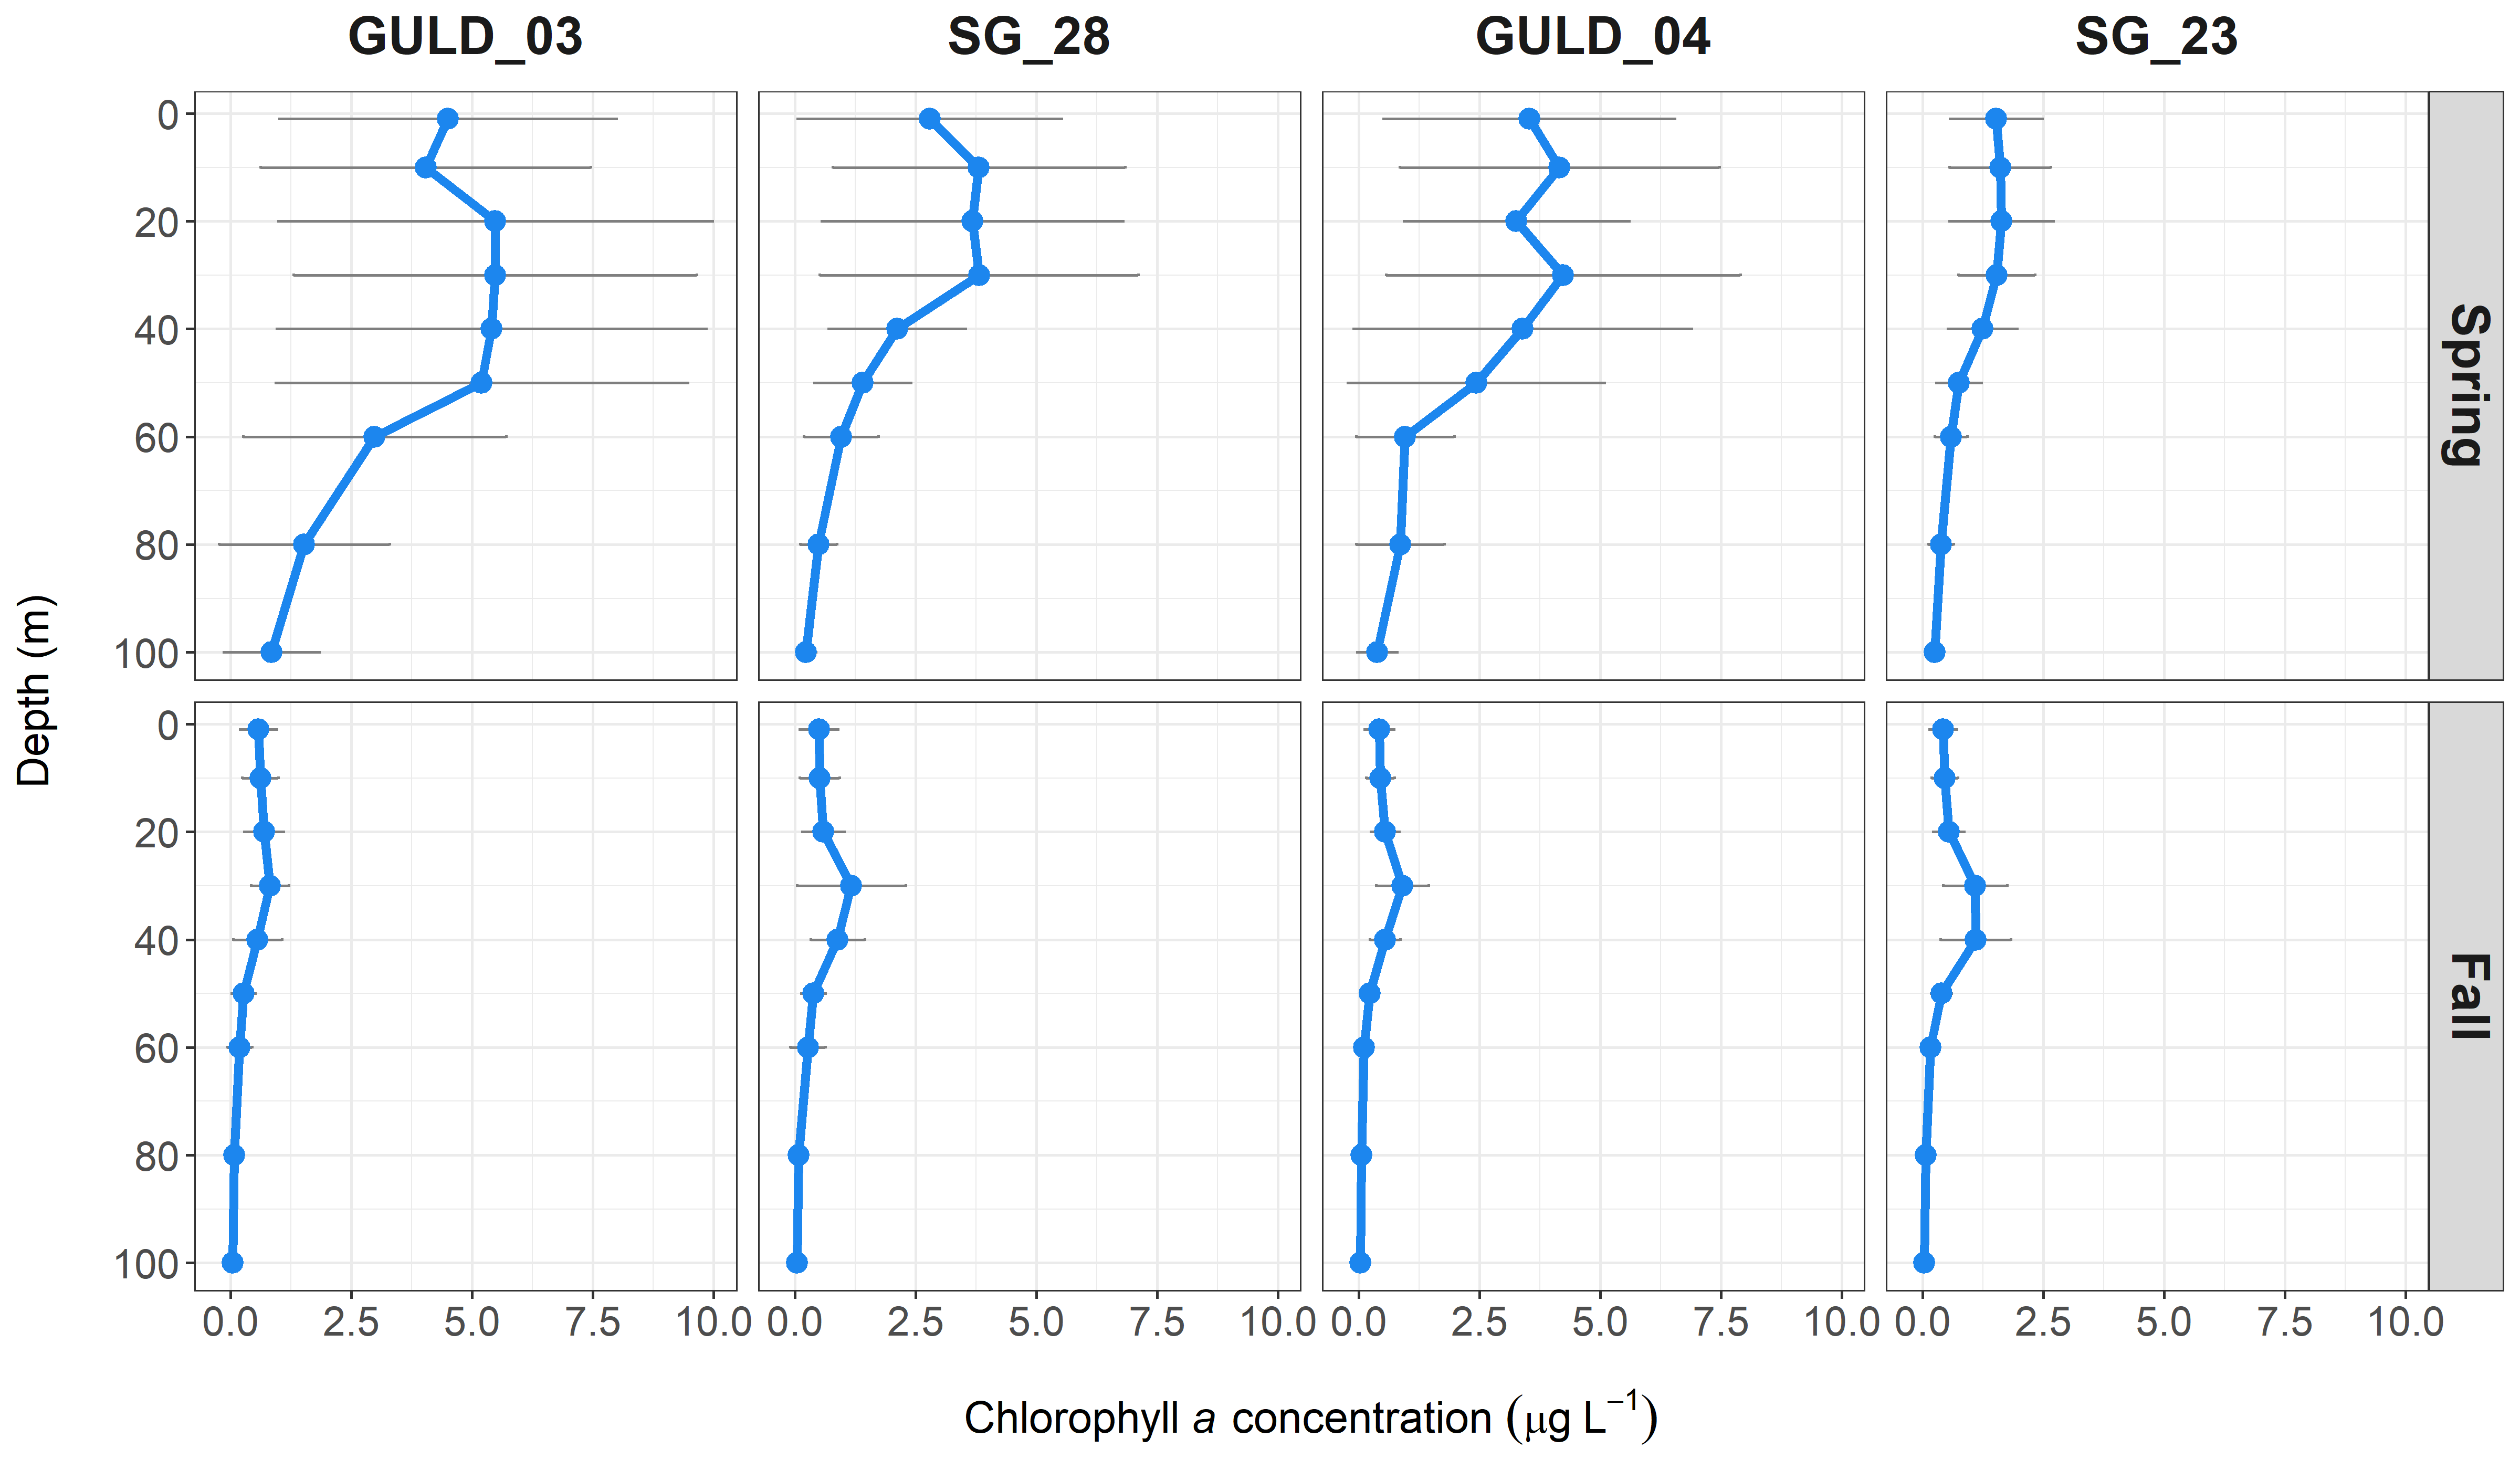
\includegraphics[width=7.5in]{figure/Figure23}}{Figure \ref{fig:figure23}} 

}

\caption{Mean vertical structure in spring and fall chlorophyll \emph{a} concentration (\(\mu\)g L\textsuperscript{-1}) from the surface to 100 m depth at the four AZMP fixed stations in the Gully. Circles represent mean chlorophyll a concentration calculated at each standard nominal depth (see Table~\ref{tab:table3}) of samples. Error bars are \(\pm\) standard deviation.}\label{fig:figure23}
\end{figure}
\end{landscapepage}
\clearpage


\begin{figure}[htb]

{\centering \pdftooltip{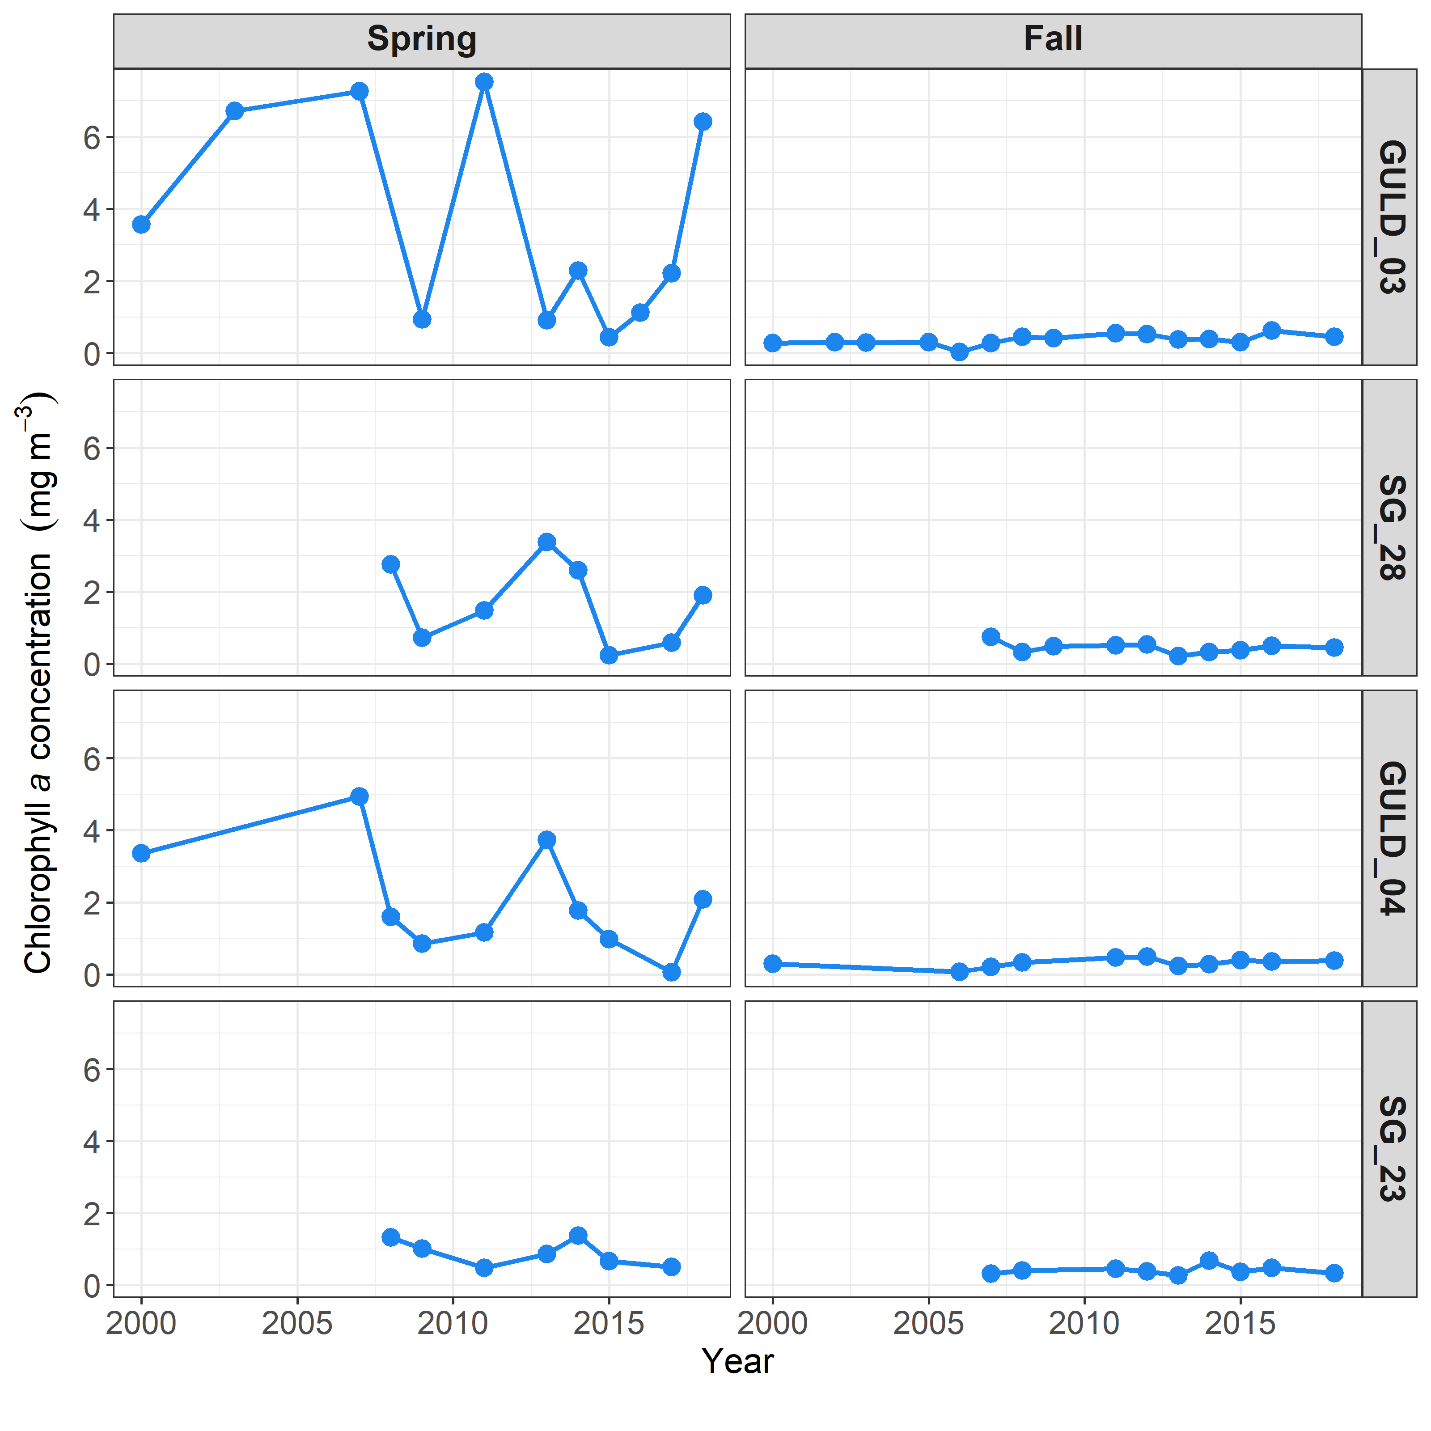
\includegraphics[width=6in]{figure/Figure24}}{Figure \ref{fig:figure24}} 

}

\caption{Vertically-integrated chlorophyll \emph{a} concentration (mg m\textsuperscript{-3}) from the top 100 m sampled in the spring (April) and fall (September and October) at the four AZMP fixed stations in the Gully. Absent circles indicate that sampling did not occur within that particular depth interval and/or year.}\label{fig:figure24}
\end{figure}
\clearpage


\begin{figure}[htb]

{\centering \pdftooltip{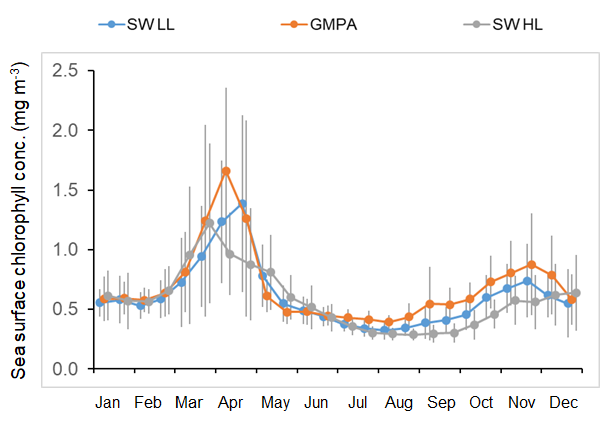
\includegraphics[width=6in]{figure/Figure25}}{Figure \ref{fig:figure25}} 

}

\caption{Remotely-sensed bi-monthly average sea surface chlorophyll concentrations (1998 to 2018, \(\pm\) S.D.) in the slope water satellite areas off the eastern (SW LL) and central (SW HL) Scotian Shelf and in the Gully MPA (GMPA).}\label{fig:figure25}
\end{figure}
\clearpage


\begin{figure}[htb]

{\centering \pdftooltip{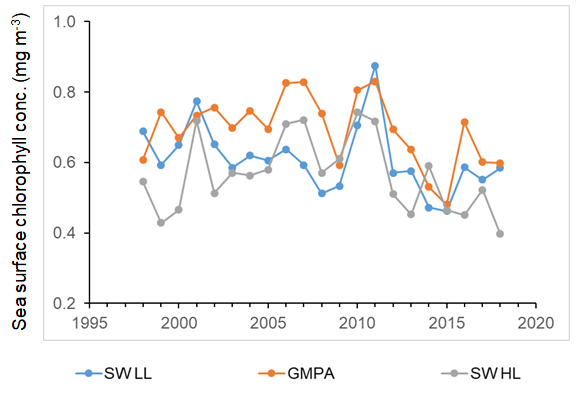
\includegraphics[width=6in]{figure/Figure26}}{Figure \ref{fig:figure26}} 

}

\caption{Time series for remotely-sensed annual average sea surface chlorophyll concentrations between 1998 and 2018 in the slope water satellite areas off the eastern (SW LL) and central (SW HL) Scotian Shelf and in the Gully MPA (GMPA).}\label{fig:figure26}
\end{figure}
\clearpage


\begin{figure}[htb]

{\centering \pdftooltip{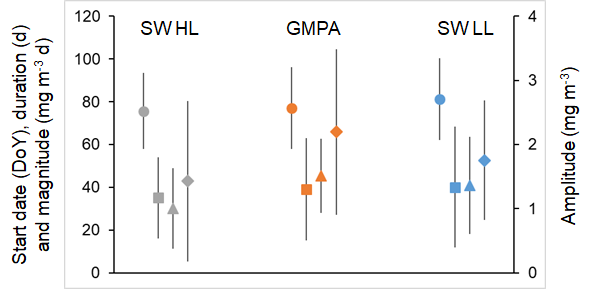
\includegraphics[width=6in]{figure/Figure27}}{Figure \ref{fig:figure27}} 

}

\caption{Average values (1998 to 2018, \(\pm\) S.D.) of the spring bloom metrics derived from the time shifted Gaussian functions fitted to the spring peaks of sea surface chlorophyll concentration in the slope water areas off the central (SW HL) and eastern (SW LL) Scotian Shelf and the Gully MPA (GMPA). Filled circles, squares, triangles and diamonds represent values for bloom start dates, durations, magnitudes and amplitudes, respectively.}\label{fig:figure27}
\end{figure}
\clearpage


\begin{figure}[htb]

{\centering \pdftooltip{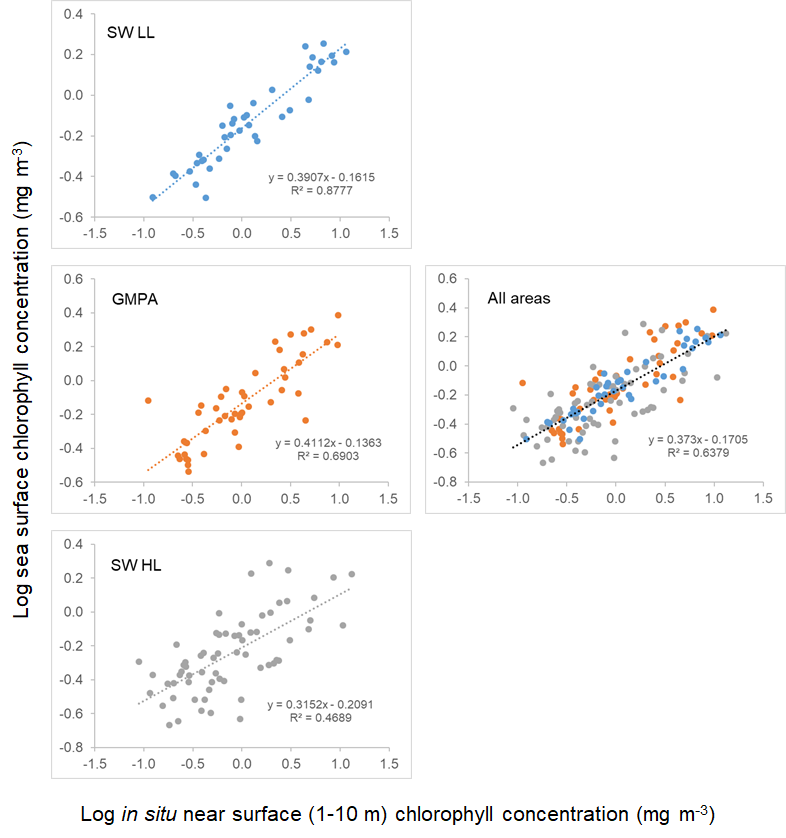
\includegraphics[width=6in]{figure/Figure28}}{Figure \ref{fig:figure28}} 

}

\caption{Relationships between \emph{in situ} measurements of chlorophyll concentrations in the 0 to 10 m depth range at stations throughout the satellite areas (SW LL, GMPA, SW HL) and remotely-sensed sea surface chlorophyll concentrations averaged for the appropriate months/years.}\label{fig:figure28}
\end{figure}
\clearpage


\begin{figure}[htb]

{\centering \pdftooltip{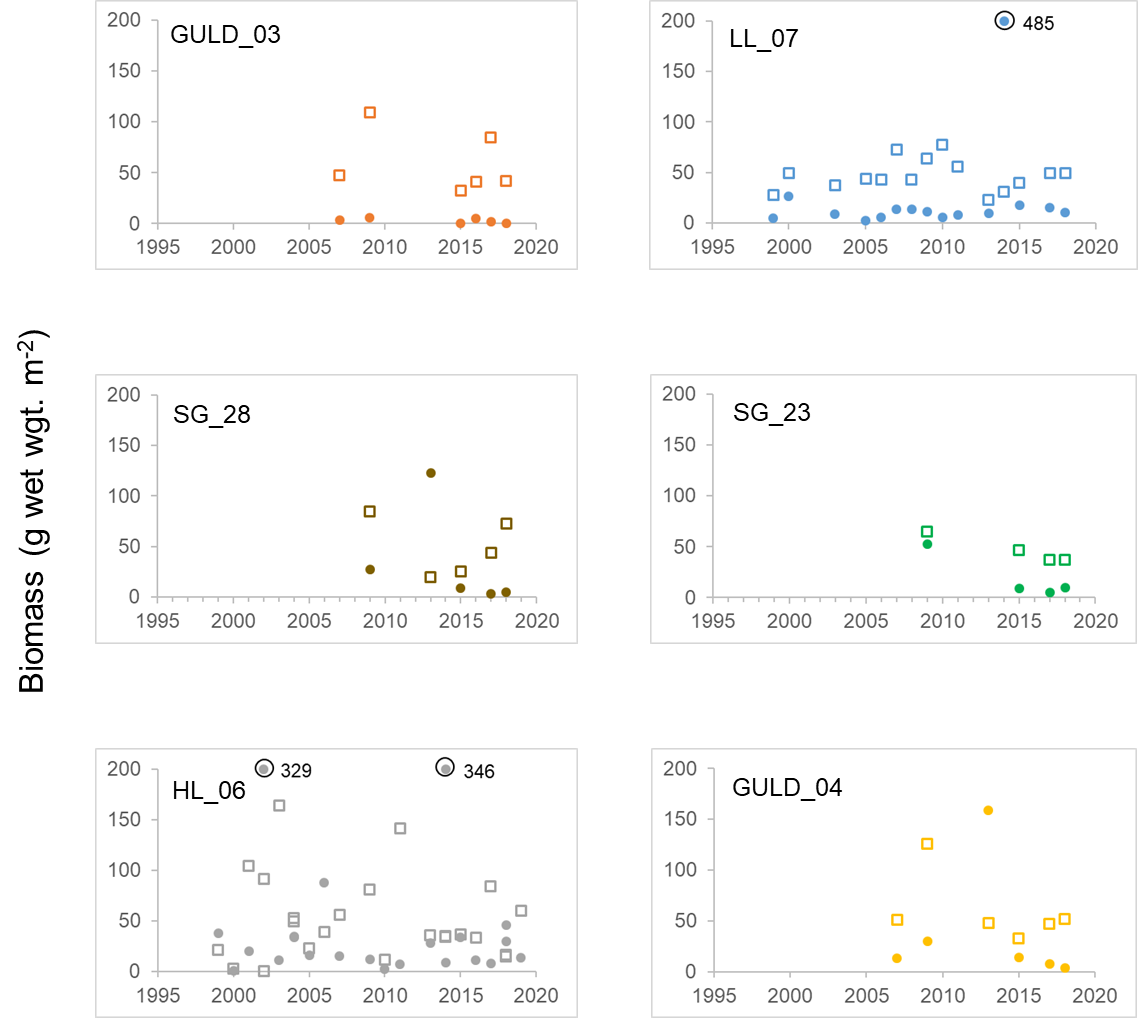
\includegraphics[width=6in]{figure/Figure29}}{Figure \ref{fig:figure29}} 

}

\caption{Time series for bulk wet weight biomass of large (\textgreater1 cm, filled circles) and small (\textless1 cm, open squares) zooplankton in spring at stations upstream (LL\_07) and downstream (HL\_06) of the Gully, within the Gully (GULD\_03) and across the Gully mouth (SG\_28, GULD\_04, SG\_23).}\label{fig:figure29}
\end{figure}
\clearpage


\begin{figure}[htb]

{\centering \pdftooltip{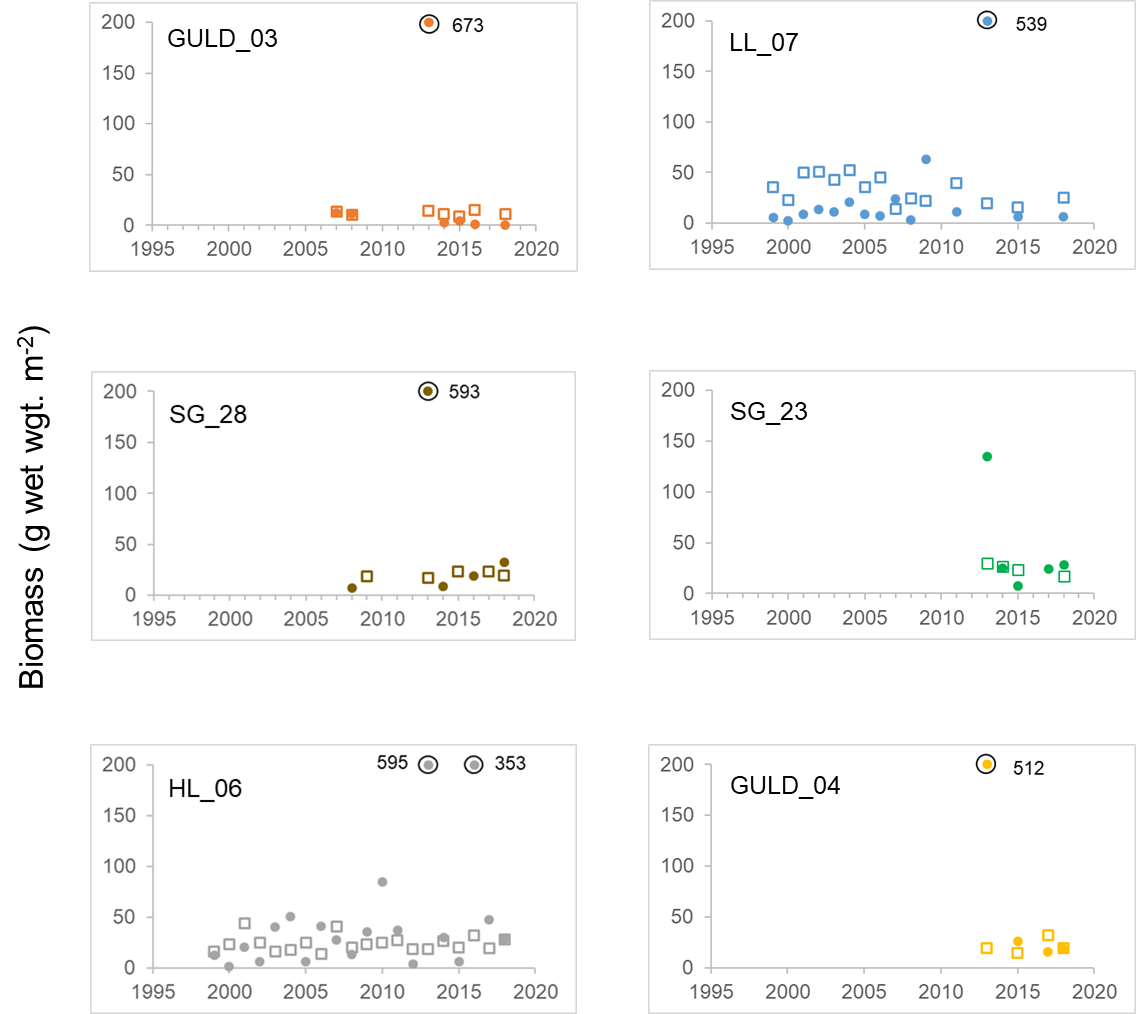
\includegraphics[width=6in]{figure/Figure30}}{Figure \ref{fig:figure30}} 

}

\caption{Time series for bulk wet weight biomass of large (\textgreater1 cm, filled circles) and small (\textless1 cm, open squares) zooplankton in fall at stations upstream (LL\_07) and downstream (HL\_06) of the Gully, within the Gully (GULD\_03) and across the Gully mouth (SG\_28, GULD\_04, SG\_23).}\label{fig:figure30}
\end{figure}
\clearpage


\begin{figure}[htb]

{\centering \pdftooltip{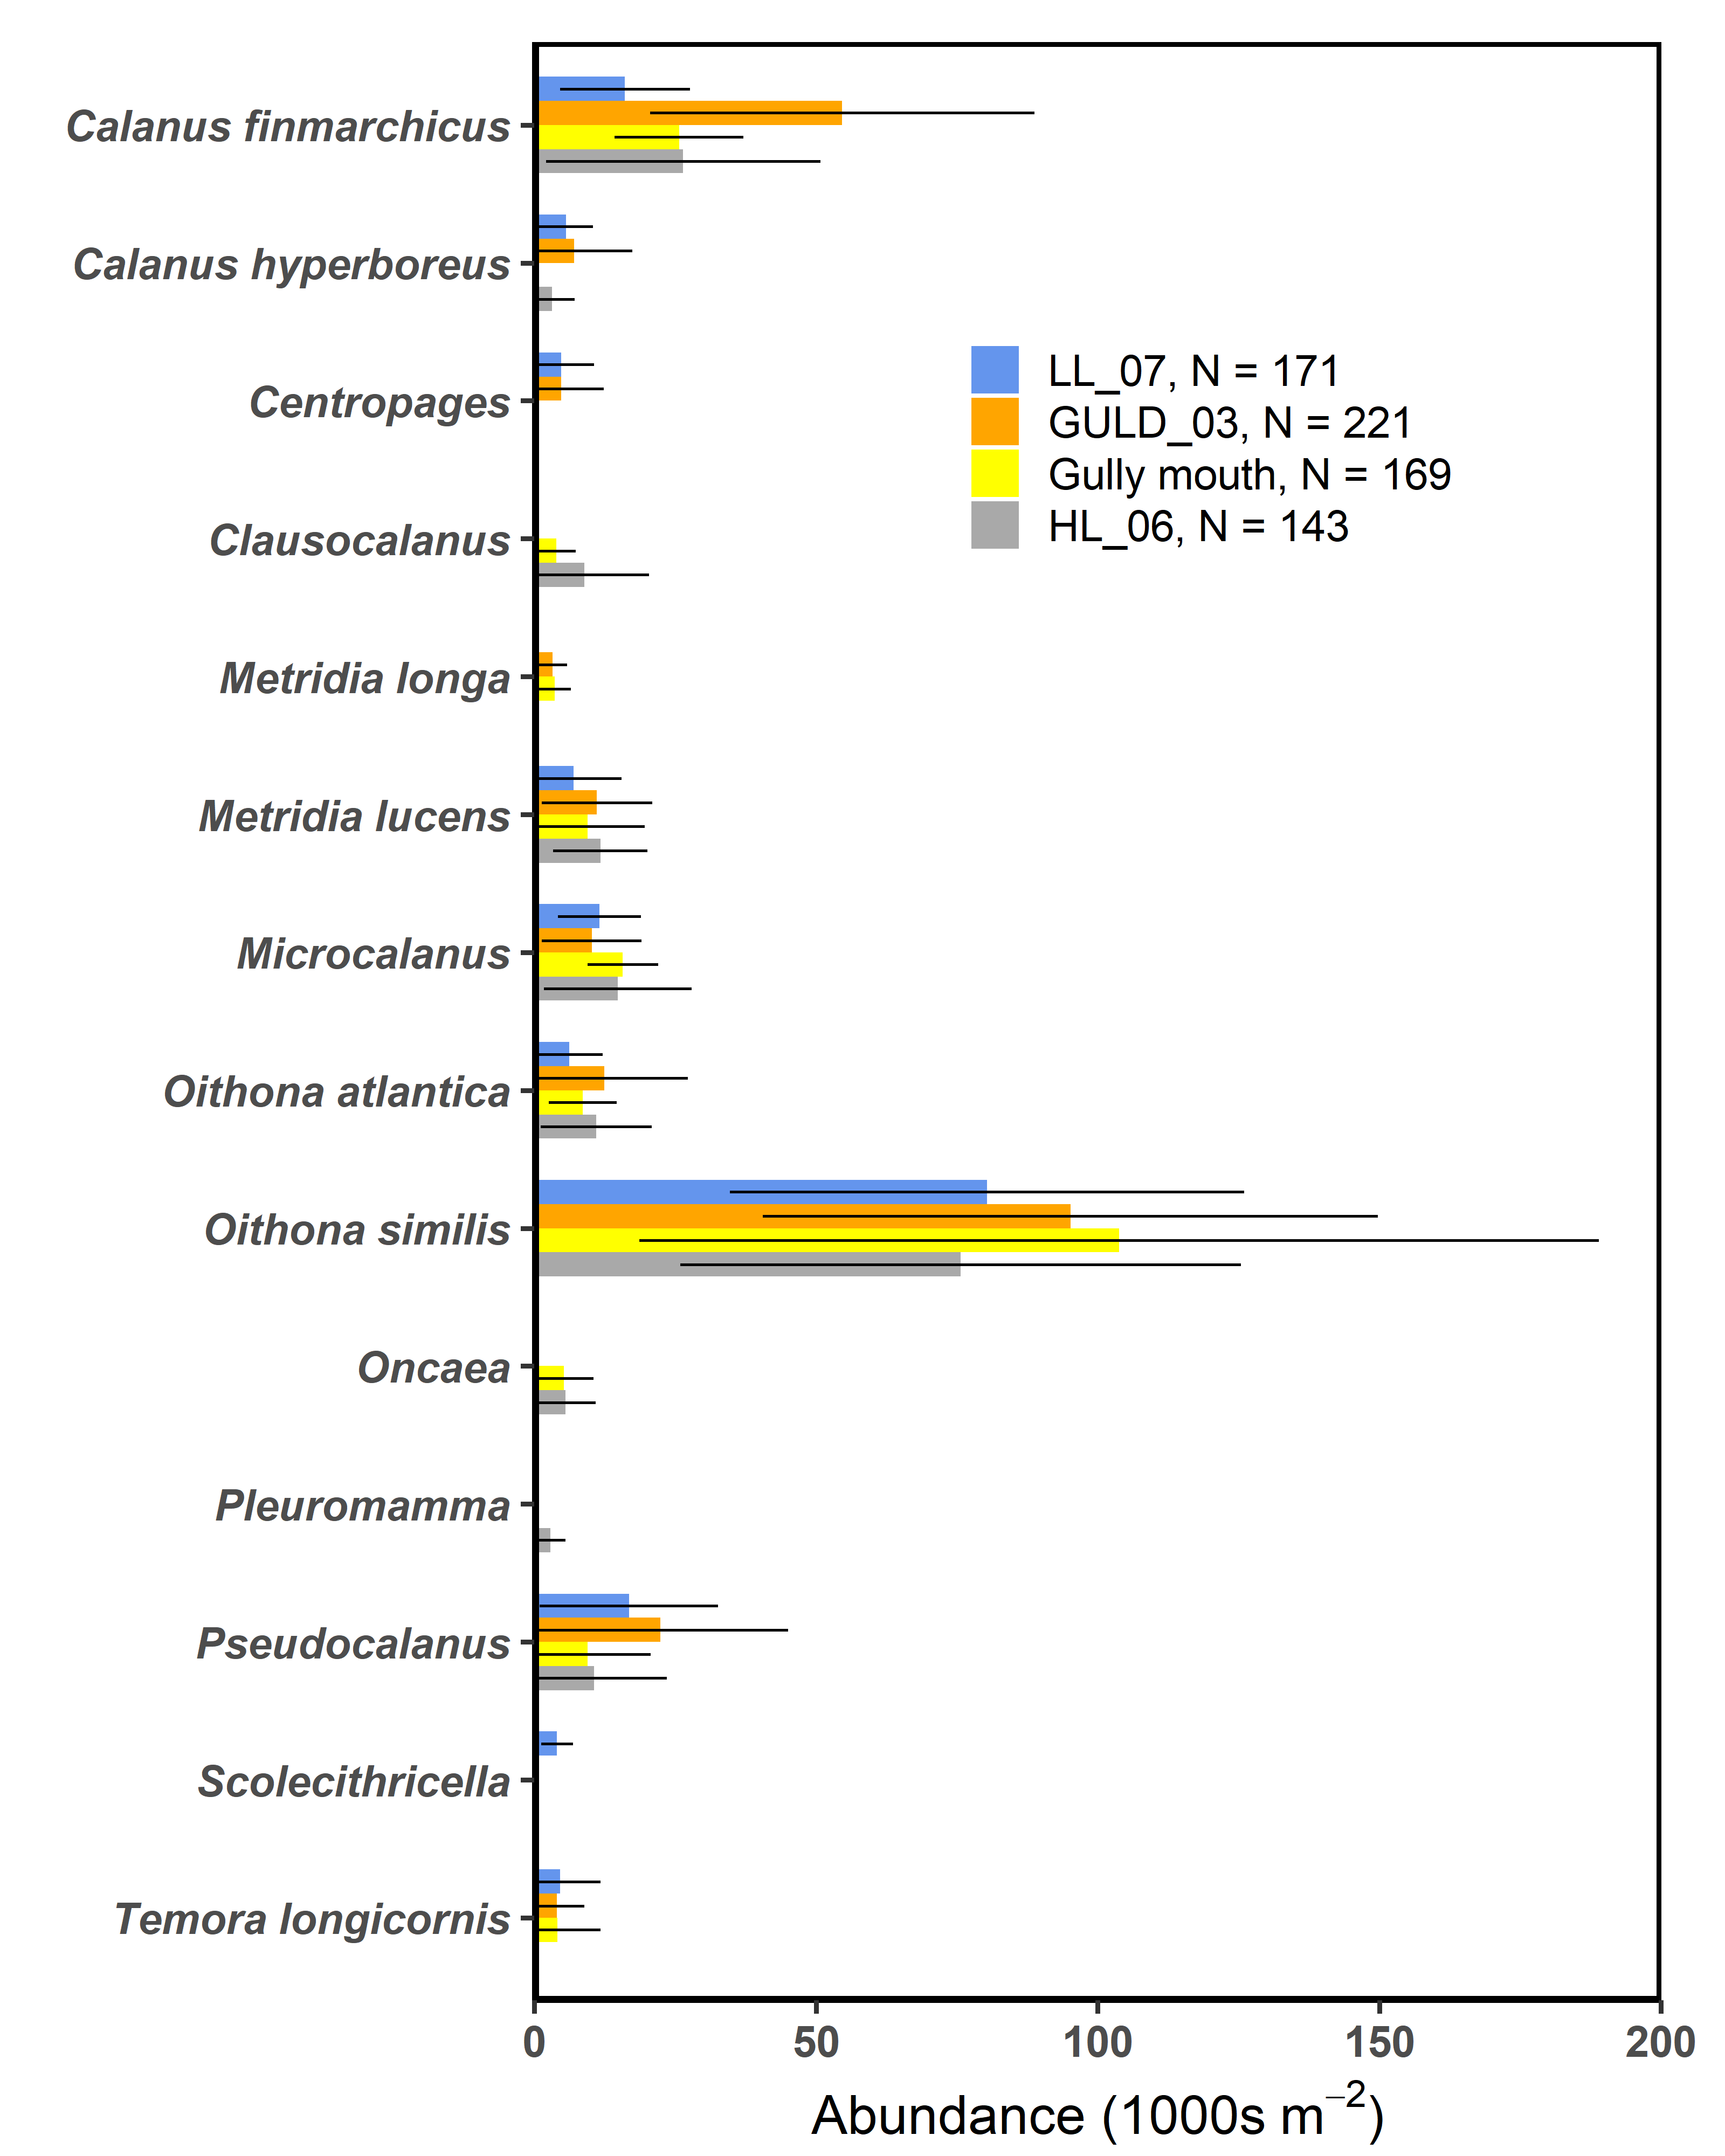
\includegraphics[width=5.5in]{figure/Figure31}}{Figure \ref{fig:figure31}} 

}

\caption{Average spring abundances of the ten most abundant copepod taxa at stations at the shelf-break upstream (LL\_07) and downstream (HL\_06) of the Gully, and at one station within the Gully (GULD\_03) and averaged over three stations across the Gully mouth (SG\_28, GULD\_04, and SG\_23). The numbers (N) in the legend represent the sums of the ten most abundant taxa at each location with units of 1000s m\textsuperscript{-2}.}\label{fig:figure31}
\end{figure}
\clearpage


\begin{figure}[htb]

{\centering \pdftooltip{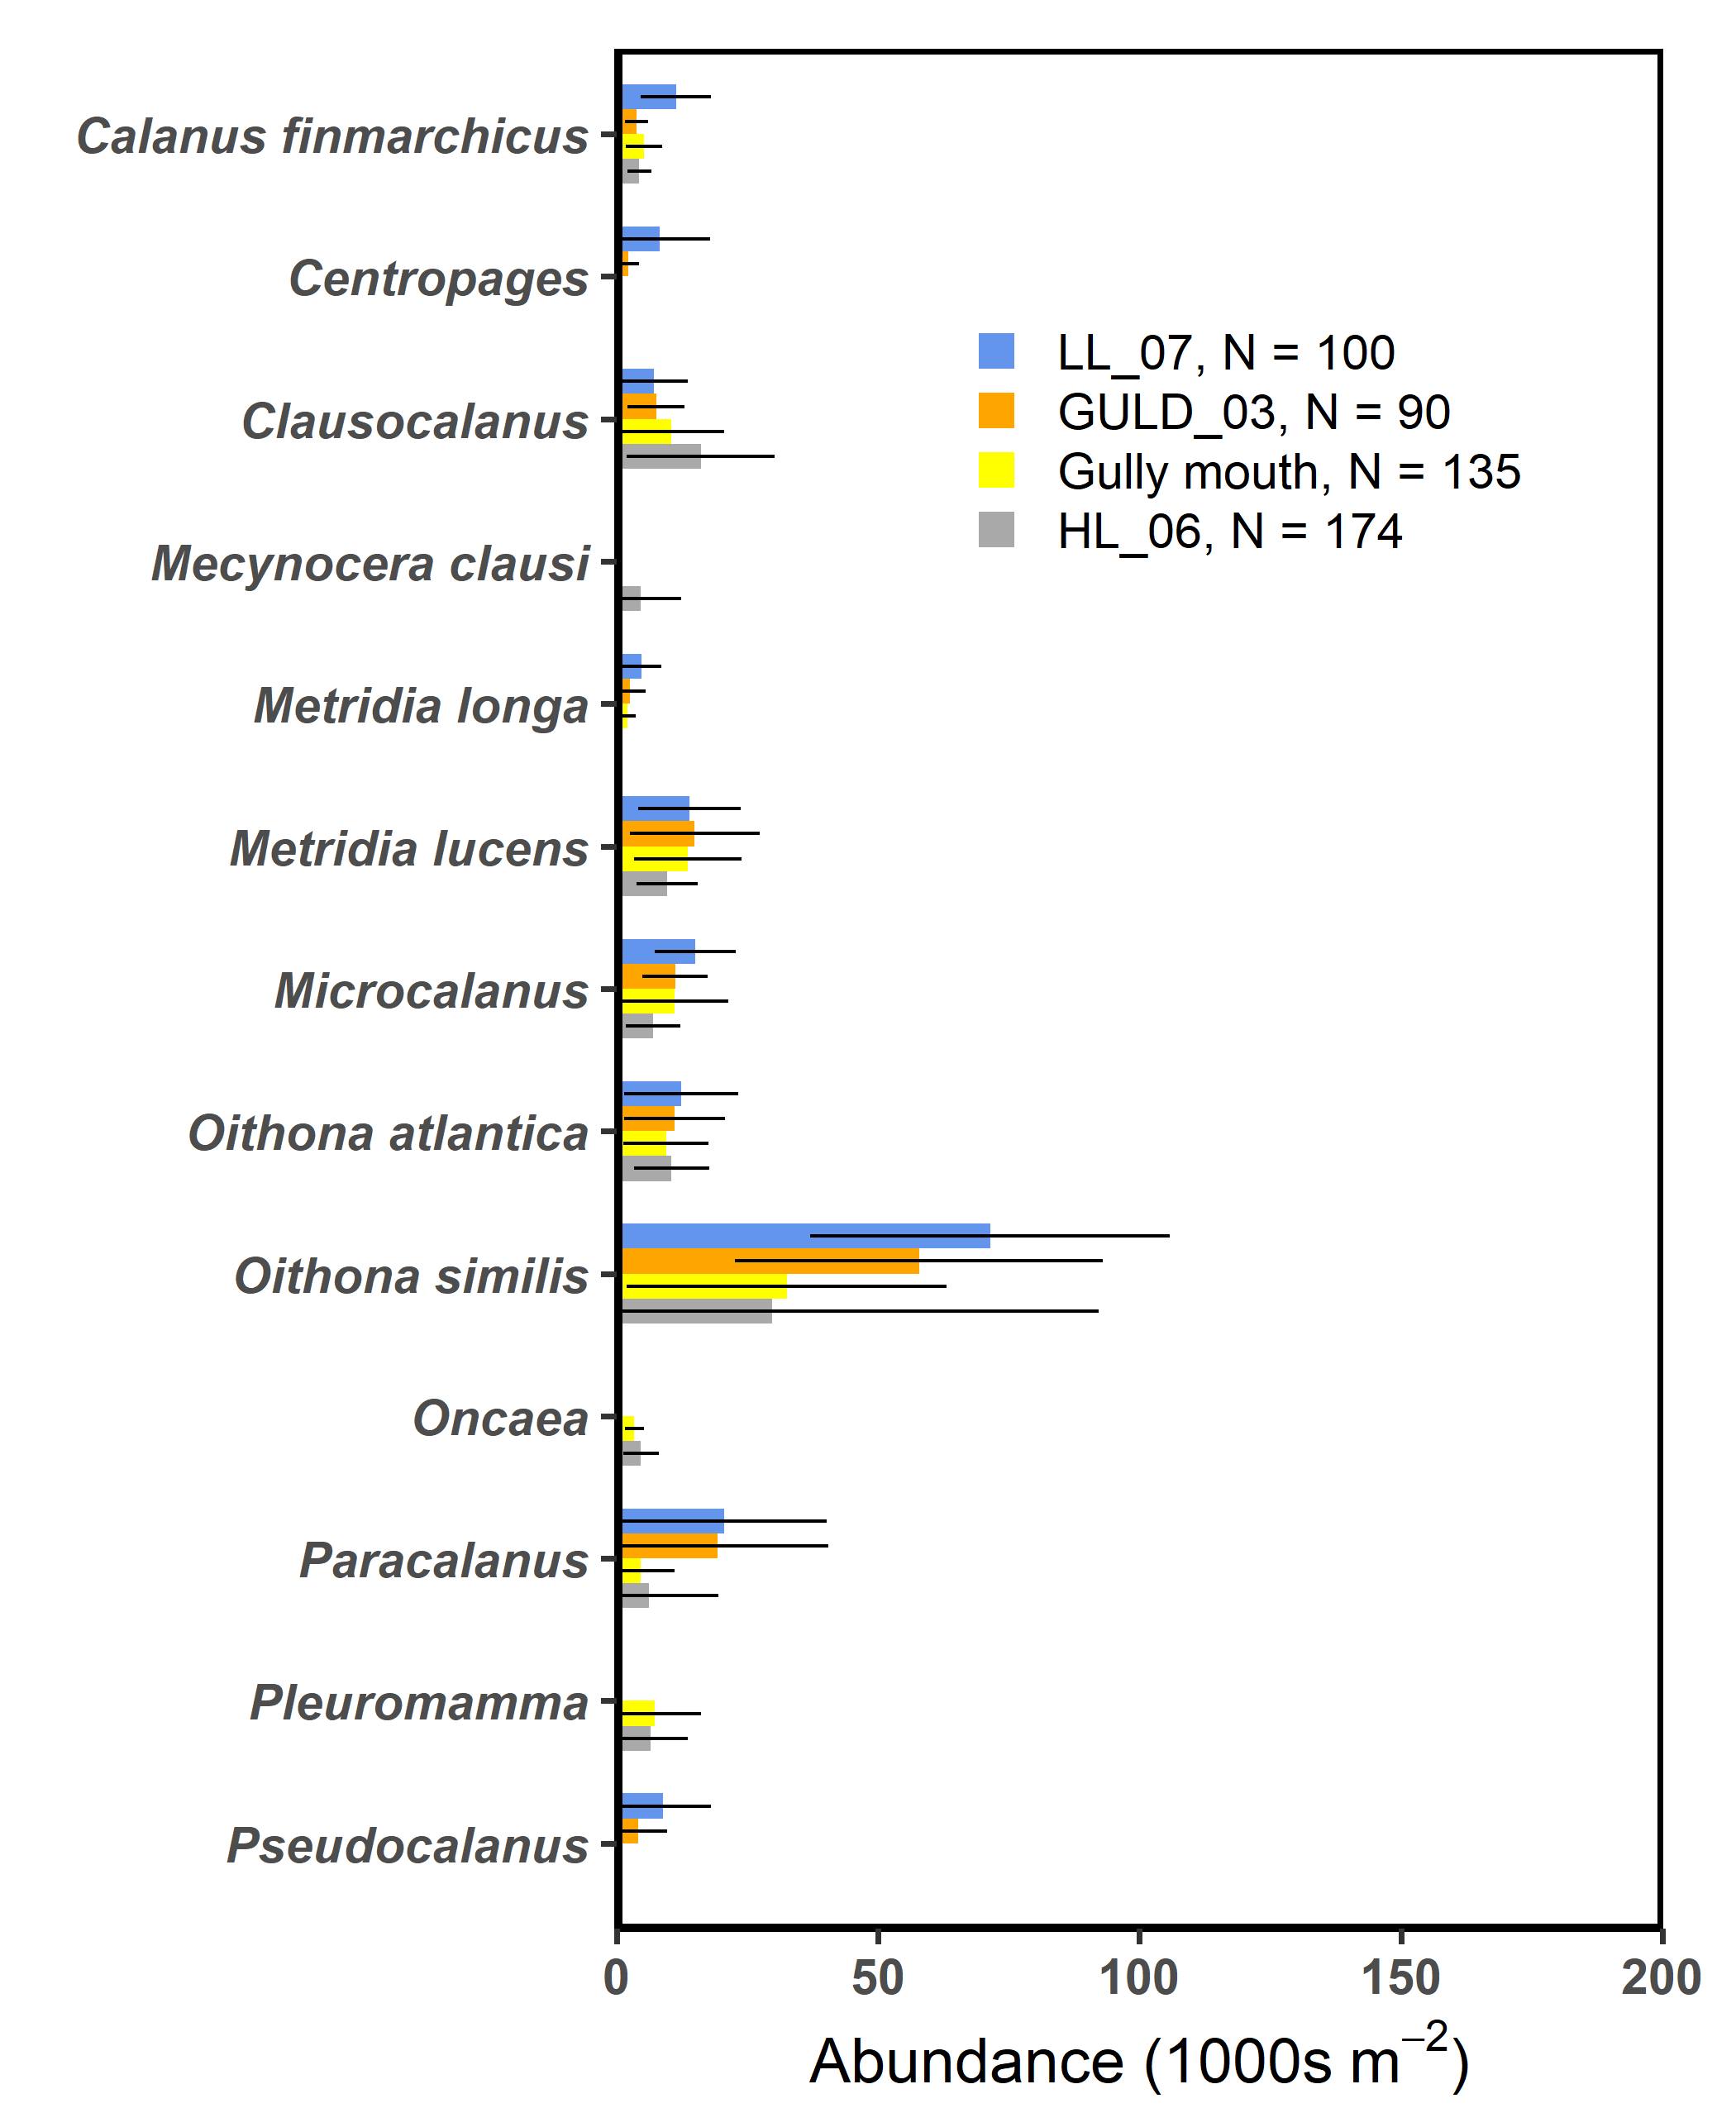
\includegraphics[width=5.5in]{figure/Figure32}}{Figure \ref{fig:figure32}} 

}

\caption{Average fall abundances of the ten most abundant copepod taxa at stations at the shelf-break upstream (LL\_07) and downstream (HL\_06) of the Gully, and at one station within the Gully (GULD\_03) and averaged over three stations across the Gully mouth (SG\_28, GULD\_04, and SG\_23). The numbers (N) in the legend represent the sums of the ten most abundant taxa at each location with units of 1000s m\textsuperscript{-2}.}\label{fig:figure32}
\end{figure}
\clearpage


\begin{landscapepage}
\begin{figure}[htb]

{\centering \pdftooltip{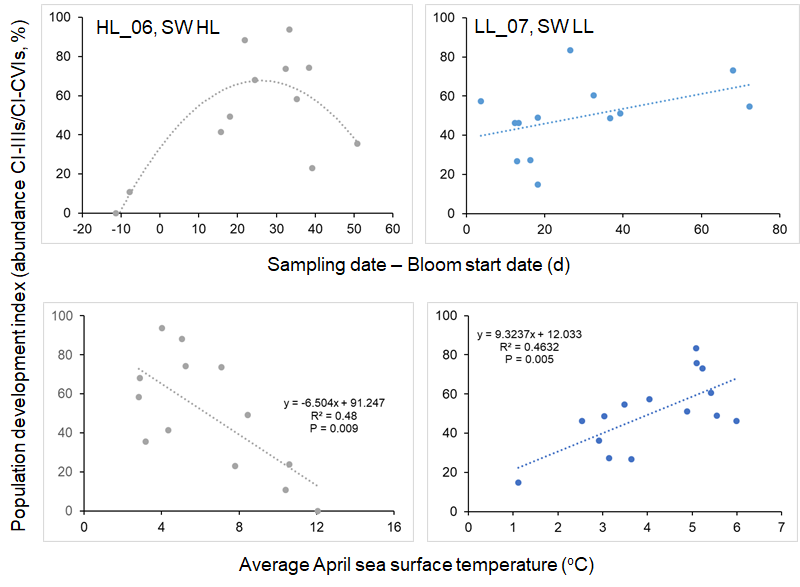
\includegraphics[width=7.5in]{figure/Figure33}}{Figure \ref{fig:figure33}} 

}

\caption{Relationships between the Population Development Index (Abundance CI-III/Abundance CI-VI, \%) for \emph{Calanus finmarchicus} populations versus sampling date minus spring bloom initiation date (top row), and April sea surface temperature (bottom row), for HL\_06, SW HL and LL\_07, SW LL.}\label{fig:figure33}
\end{figure}
\end{landscapepage}
\clearpage


\begin{figure}[htb]

{\centering \pdftooltip{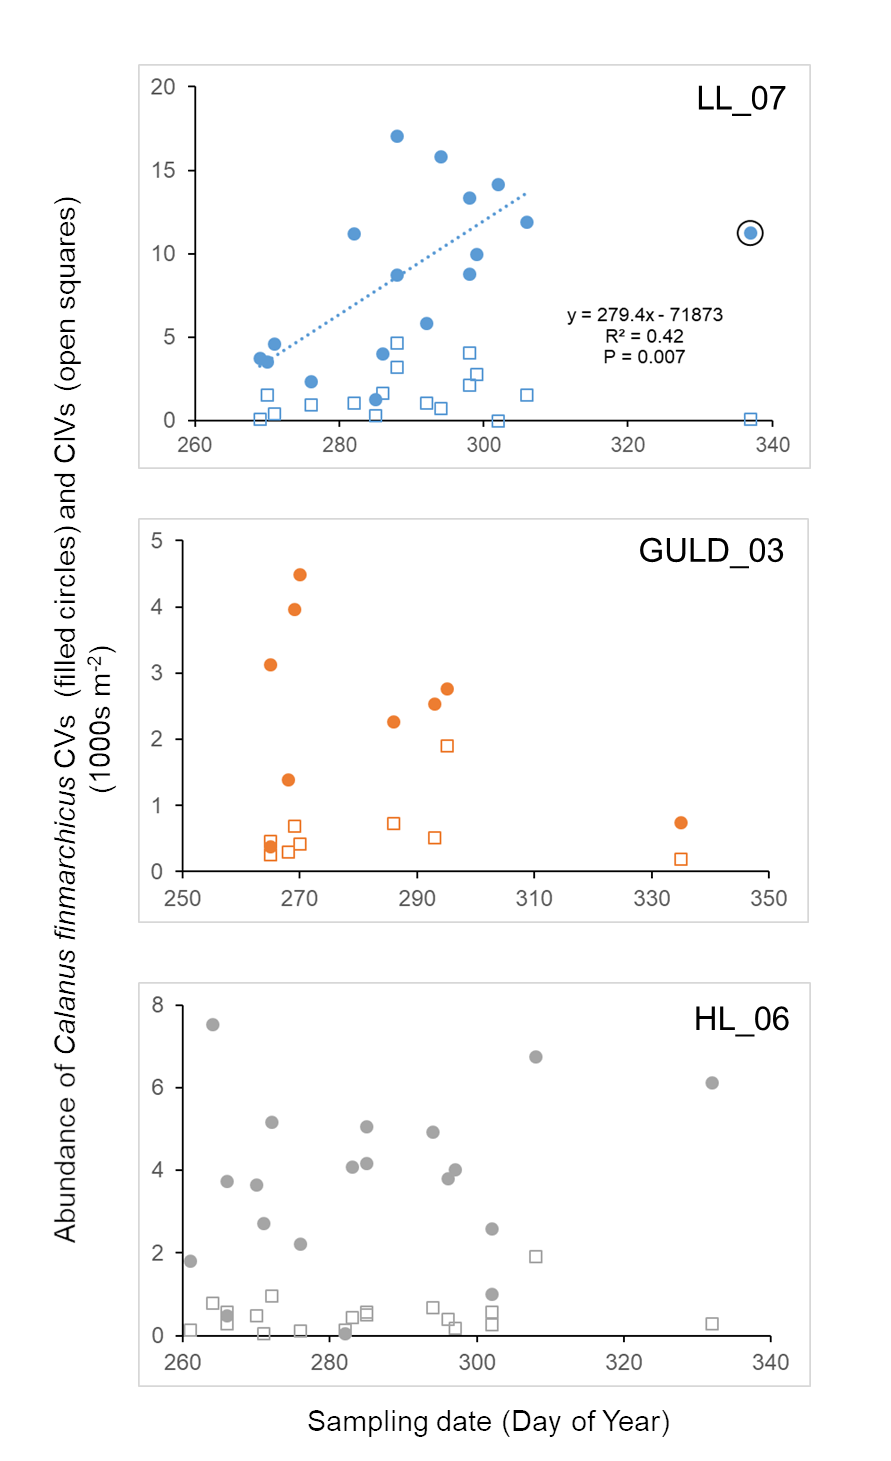
\includegraphics[width=4.75in]{figure/Figure34}}{Figure \ref{fig:figure34}} 

}

\caption{Abundance of stage CV (filled circles) and stage CIV (open squares) \emph{C. finmarchicus} versus sampling date at LL\_07, GULD\_03 and HL\_06 in fall between 1999 and 2018. Note that the outlier circled in black from 2017 at LL\_07 was excluded from the only significant correlation between abundance and sampling date.}\label{fig:figure34}
\end{figure}
\clearpage
\end{document}
